%%%%%%%%%%%%%%%%%%%%%%%%%%%%%%%%%%%%
% Tables
%%%%%%%%%%%%%%%%%%%%%%%%%%%%%%%%%%%%
\begin{landscape}
\begin{table}[H]
\centering
\caption{CPS Summary Statistics \label{tab:sumstat1}}
\centering
\begin{threeparttable}
\begin{tabular}[t]{lcccc}
\toprule
\multicolumn{1}{c}{ } & \multicolumn{1}{c}{\textbf{Overall}} & \multicolumn{3}{c}{\textbf{By Generation}} \\
\cmidrule(l{3pt}r{3pt}){2-2} \cmidrule(l{3pt}r{3pt}){3-5}
\textbf{Characteristic} & \makecell[c]{\textbf{All Sample} \\N = 318,404} & \makecell[c]{\textbf{First} \\N=40,033} & \makecell[c]{\textbf{Second} \\N=199,294} & \makecell[c]{\textbf{Third} \\N=79,077}\\
\midrule
Female & 0.49 & 0.53 & 0.49 & 0.49\\
Asian & 0.65 & 0.96 & 0.73 & 0.31\\
Age & 8.4 (5.1) & 10.9 (4.5) & 8.3 (5.1) & 7.7 (5.0)\\
College Graduate:\ \ 	 Father & 0.52 & 0.59 & 0.52 & 0.50\\
College Graduate:\ \ 	 Mother & 0.52 & 0.56 & 0.51 & 0.52\\
Total Family Income\ \ 	 (1999 dollars) & 87,031 (84,797) & 75,815 (74,489) & 88,295 (88,411) & 89,436 (80,051)\\
\bottomrule
\end{tabular}
\begin{tablenotes}
\item[1] The samples include children ages 17 and below who live in intact families. First-generation Asian immigrant children that were born in a Asian country. Native-born second-generation Asian immigrant children with at least one parent born in a Asian country. Finally, native-born third generation Asian immigrant children with native-born parents and at least one grand parent born in a Asian country.
\item[2] Data source is the 2004-2021 Current Population Survey.
\end{tablenotes}
\end{threeparttable}
\end{table}

\end{landscape}

\newpage
\pagebreak

\begin{table}

\caption{Current Population Survey (CPS) Summary Statistics \label{tab:sumstat-adults}}
\centering
\begin{threeparttable}
\begin{tabular}[t]{lccc}
\toprule
\multicolumn{1}{c}{ } & \multicolumn{1}{c}{\textbf{Overall}} & \multicolumn{2}{c}{\textbf{By Generation}} \\
\cmidrule(l{3pt}r{3pt}){2-2} \cmidrule(l{3pt}r{3pt}){3-4}
\textbf{Characteristic} & \makecell[c]{\textbf{All Sample} \\N = 48,153} & \makecell[c]{\textbf{First} \\N=35,728} & \makecell[c]{\textbf{Second} \\N=12,425}\\
\midrule
Female & 0.56 & 0.58 & 0.50\\
Asian & 0.90 & 0.96 & 0.73\\
Age & 46 (17) & 49 (16) & 38 (17)\\
Years of Education & 14.0 (3.5) & 13.9 (3.8) & 14.5 (2.5)\\
Total Family Income\ \ 	 (1999 dollars) & 68,121 (71,266) & 66,093 (70,444) & 73,950 (73,269)\\
\bottomrule
\end{tabular}
\begin{tablenotes}
\item[1] The samples include people of Asian ancestry ages 18 and above. First-generation Asian immigrants were born in a Asian country. Native-born second-generation Asian immigrants have at least one parent born in a Asian country. 
\item[2] Data source is the 2004-2021 Current Population Survey.
\end{tablenotes}
\end{threeparttable}
\end{table}


\newpage
\pagebreak

\begin{table}[H]
\centering\centering
\caption{Main Effect of Proxy on Second-Generation's Asian Self-identification \label{tab:hispbyproxy}}
\centering
\fontsize{12}{14}\selectfont
\begin{tabular}[c]{>{}lllll}
\toprule
Parents Type & All & Asian-Asian & Asian-White & White-Asian\\
\midrule
\textbf{Proxy:} &  &  &  & \\
\hspace{1em}\textbf{Mother} & 0.72 & 0.97 & 0.37 & 0.3\\
\hspace{1em}\textbf{Father} & 0.72 & 0.97 & 0.39 & 0.29\\
\hspace{1em}\textbf{Self} & 0.87 & 0.97 & 0.23 & 0.31\\
\hspace{1em}\textbf{Others} & 0.88 & 0.96 & 0.6 & 0.54\\
\bottomrule
\end{tabular}
\end{table}


\pagebreak
\newpage

\begin{table}[H]
\centering\centering
\caption{Asian Self-identification by Generation \label{tab:hispbygen}}
\centering
\begin{threeparttable}
\begin{tabular}[t]{>{}lcccc}
\toprule
  & \specialcell{Self-identify \\ as Asian} & \specialcell{Self-identify as \\ non-Asian} & \specialcell{\% Self-identify \\ as Asian} & \specialcell{\% Self-identify \\ as non-Asian}\\
\midrule
\textbf{1st Gen.} & 14,811 & 688 & 0.96 & 0.04\\
\textbf{2nd Gen.} & 58,756 & 21,381 & 0.73 & 0.27\\
\hspace{1em}\textbf{Asian on:} &  &  &  \vphantom{1} & \\
\hspace{1em}\hspace{1em}\textbf{Both Sides} & 49,118 & 1,717 & 0.97 & 0.03\\
\hspace{1em}\hspace{1em}\textbf{One Side} & 9,638 & 19,664 & 0.33 & 0.67\\
\addlinespace
\textbf{3rd Gen.} & 10,394 & 23,048 & 0.31 & 0.69\\
\hspace{1em}\textbf{Asian on:} &  &  &  & \\
\hspace{1em}\hspace{1em}\textbf{Both Sides} & 5,428 & 316 & 0.94 & 0.06\\
\hspace{1em}\hspace{1em}\textbf{One Side} & 3,030 & 9,213 & 0.25 & 0.75\\
\bottomrule
\end{tabular}
\begin{tablenotes}
\item[1] The samples include children ages 17 and below who live in intact families. First-generation Asian immigrant children that were born in a Asian country. Native-born second-generation Asian immigrant children with at least one parent born in a Asian country. Finally, native-born third-generation Asian immigrant children with native-born parents and at least one grandparent born in a Asian country.
\item[2] Data source is the 2004-2021 Current Population Survey.
\end{tablenotes}
\end{threeparttable}
\end{table}


\newpage
\pagebreak

\begin{table}[H]
\centering\centering
\caption{Asian Self-identification by Generation \label{tab:hispbygen-adults}}
\centering
\begin{threeparttable}
\begin{tabular}[t]{>{}lcccc}
\toprule
  & \specialcell{Self-identify \\ as Asian} & \specialcell{Self-identify as \\ non-Asian} & \specialcell{\% Self-identify \\ as Asian} & \specialcell{\% Self-identify \\ as non-Asian}\\
\midrule
\textbf{1st Gen.} & 275,516 & 11,037 & 0.96 & 0.04\\
\textbf{2nd Gen.} & 74,345 & 28,027 & 0.73 & 0.27\\
\hspace{1em}\textbf{Asian on:} &  &  &  & \\
\hspace{1em}\hspace{1em}\textbf{Both Sides} & 59,880 & 2,935 & 0.95 & 0.05\\
\hspace{1em}\hspace{1em}\textbf{One Side} & 14,465 & 25,092 & 0.37 & 0.63\\
\bottomrule
\end{tabular}
\begin{tablenotes}
\item[1] The samples include people of Asian ancestry ages 18 and above. First-generation Asian immigrants were born in a Asian country. Native-born second-generation Asian immigrants have at least one parent born in a Asian country. 
\item[2] Data source is the 2004-2021 Current Population Survey.
\end{tablenotes}
\end{threeparttable}
\end{table}


\pagebreak
\newpage

\begin{table}[H]

\caption{Relationship Between Bias and Self-Reported Hispanic identity Among Third-Generation Hispanic Immigrants: By Grandparental Type \label{regtab-bygrandparents}}
\centering
\resizebox{\linewidth}{!}{
\begin{threeparttable}
\begin{tabular}[t]{lcccc}
\toprule
\multicolumn{1}{c}{ } & \multicolumn{4}{c}{Number of Hispanic Grandparents} \\
\cmidrule(l{3pt}r{3pt}){2-5}
  & \specialcell{(1) \\ One} & \specialcell{(2) \\ Two} & \specialcell{(3) \\ Three} & \specialcell{(4) \\ Four}\\
\midrule
Bias & -0.04 & 0.03 & 0.19 & -0.14*\\
 & (0.11) & (0.09) & (0.26) & (0.07)\\
Female & -0.01 & 0.00 & -0.01 & 0.00\\
 & (0.01) & (0.01) & (0.01) & (0.01)\\
College Graduate: Mother & -0.11*** & -0.07*** & 0.02 & -0.02\\
 & (0.03) & (0.02) & (0.02) & (0.01)\\
College Graduate: Father & -0.11*** & -0.08*** & 0.02 & -0.03*\\
 & (0.03) & (0.01) & (0.01) & (0.01)\\
\midrule
Observations & 55,051 & 74,100 & 12,194 & 57,646\\
Year $\times$ Region FE & X & X & X & X\\
\bottomrule
\multicolumn{5}{l}{\rule{0pt}{1em}* p $<$ 0.1, ** p $<$ 0.05, *** p $<$ 0.01}\\
\end{tabular}
\begin{tablenotes}
\small
\item[1] \footnotesize{Each column is an estimation of equation (\ref{eq:identity_reg_bias}) restricted to third-generation Hispanic immigrants by 
                      number of Hispanic grandparents with region × year fixed effects. 
                      I include controls for sex, quartic age, fraction of Hispanics in a state, and parental education.
                      Standard errors are clustered on the state level.}
\item[2] \footnotesize{The samples include third-generation Hispanic children ages 17 and below who live in intact families. 
                      Native-born third-generation Hispanic 
                      immigrant children with at least one grandparent born in a Spanish-speaking 
                      country.}
\item[3] \footnotesize{Data source is the 2004-2021 Current Population Survey.}
\end{tablenotes}
\end{threeparttable}}
\end{table}


\pagebreak
\newpage

\begin{table}[H]
\centering\centering
\caption{Relationship Between Bias and Migration \label{regtab-mig-01}}
\centering
\resizebox{0.7\textwidth}{!}{
\begin{threeparttable}
\begin{tabular}[t]{lccc}
\toprule
  & \specialcell{(1) \\ Migrated from \\ Birth Place} & \specialcell{(2) \\ Migrated from \\ Birth Place} & \specialcell{(3) \\ $Bias_{ist} - Bias_{ilb}$}\\
\midrule
$Bias_{st}$ & 0.13* &  & \\
 & (0.07) &  & \\
$Bias_{lb}$ &  & -0.03 & \\
 &  & (0.17) & \\
Asian &  &  & 0.02\\
 &  &  & (0.04)\\
Female & 0.00 & -0.01 & 0.00\\
 & (0.00) & (0.00) & (0.02)\\
College Graduate: Mother & 0.01*** & 0.00 & -0.01\\
 & (0.00) & (0.01) & (0.03)\\
College Graduate: Father & -0.03*** & -0.03*** & 0.03\\
 & (0.01) & (0.01) & (0.02)\\
\midrule
Observations & 73,563 & 41,641 & 2,075\\
Mean & 0.15 & 0.15 & -0.1\\
Year $\times$ Region FE & X &  & \\
Birthyear $\times$ Birth Region FE &  & X & \\
\bottomrule
\multicolumn{4}{l}{\rule{0pt}{1em}* p $<$ 0.1, ** p $<$ 0.05, *** p $<$ 0.01}\\
\end{tabular}
\begin{tablenotes}
\small
\item[1] \footnotesize{Each column is an estimation of equations (\ref{eq:migration-3}) in column (1), 
                      (\ref{eq:migration-4}) in column (2), and
                      (\ref{eq:migration-5}) in column (3).}
\item[2] \footnotesize{Column (1) is a regression where the left hand side variable is 
                      a dummy variable that is equal to one if a person migrated from the state
                      were born in and the right hand side variable is bias the year of survey.
                      Column (2) is a regression where the left hand side variable is 
                      a dummy variable that is equal to one if a person migrated from the state
                      were born in and the right hand side variable is bias the year of birth in the state of birth.
                      Column (3) is a regression where the left hand side variable is 
                      the difference between state-level bias during the year of the survey in the current state the 
                      respondent is living in, and state-level bias during the year of birth in the state of birth 
                      and the right hand side variable is self-reported Asian identity. This regression captures
                      the selection of those that self-reported Asian identity into states with different levels of bias.
                      I include controls for sex, quartic age, parental education, fraction of Asians in a state, and region × year fixed effects.
                      Standard errors are clustered on the state level.}
\item[3] \footnotesize{The samples include children ages 17 and below who live in intact families. 
                      Native-born second-generation Asian immigrant children with both
                      parents born in a Asian country. The sample in the column (3) regression is further restricted to only those that migrated from their birth state.}
\item[4] \footnotesize{Data source is the 2004-2021 Census Data.}
\end{tablenotes}
\end{threeparttable}}
\end{table}


\pagebreak
\newpage

\begin{table}[H]
\centering\centering
\caption{Relationship Between Bias and Interethnic Marriages \label{regtab-logit-02}}
\centering
\begin{threeparttable}
\begin{tabular}[t]{lccc}
\toprule
\multicolumn{2}{c}{ } & \multicolumn{1}{c}{Asian Men} & \multicolumn{1}{c}{Asian Women} \\
\cmidrule(l{3pt}r{3pt}){3-3} \cmidrule(l{3pt}r{3pt}){4-4}
  & \specialcell{(1) \\ Interethnic} & \specialcell{(2) \\ Interethnic} & \specialcell{(3) \\ Interethnic}\\
\midrule
Bias & $0.04$*** & $-0.01$ & $0.03$**\\
 & ($0.01$) & ($0.01$) & ($0.01$)\\
College Graduate: Wife & $0.04$*** & $0.04$*** & $0.05$***\\
 & ($0.00$) & ($0.01$) & \vphantom{1} ($0.00$)\\
College Graduate: Husband & $-0.01$* & $-0.01$ & $-0.02$***\\
 & ($0.00$) & ($0.01$) & ($0.00$)\\
\midrule
Observations & $69,800$ & $52,103$ & $60,214$\\
Year $\times$ Region FE & X & X & X\\
\bottomrule
\multicolumn{4}{l}{\rule{0pt}{1em}* p $<$ 0.1, ** p $<$ 0.05, *** p $<$ 0.01}\\
\end{tabular}
\begin{tablenotes}
\small
\item[1] \footnotesize{This is the result to estimating (\ref{eq:inter-interethnic}) as a
                      linear probability model.}
\item[2] \footnotesize{I include controls for partners' sex, age, education, 
                      and years since immigrating to the United States.
                      Standard errors are clustered on the household level.}
\item[3] \footnotesize{Data source is the 2004-2020 Current Population Survey Data.}
\end{tablenotes}
\end{threeparttable}
\end{table}


\pagebreak
\newpage

\begin{center}
\begin{figure}[H]
\caption{Diagram of the Three Different Generations of Asian Immigrants.}
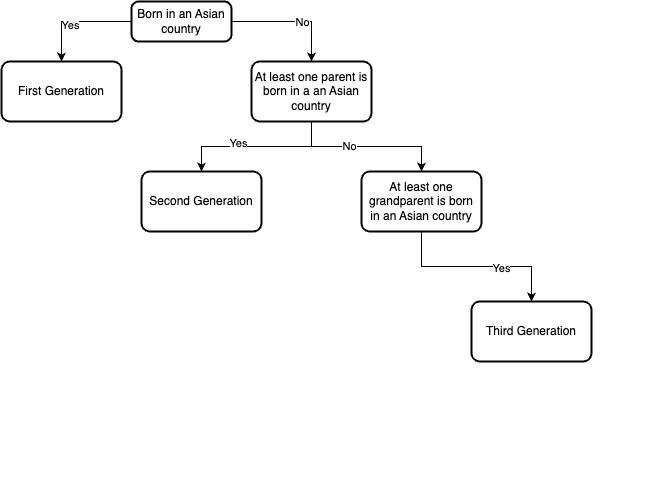
\includegraphics[width=\textwidth, height=9cm]{diag.png} 
\label{fig:diag}
\end{figure}
\hfill%
\end{center}

\begin{center}
\begin{figure}[H]
\caption{Bias and Self-reported Asian Identity in the Least and Most Biased Places} \label{fig:toptwobias}

% first
\begin{subfigure}{.9\textwidth}
\caption{Bias Over Time}
\centering
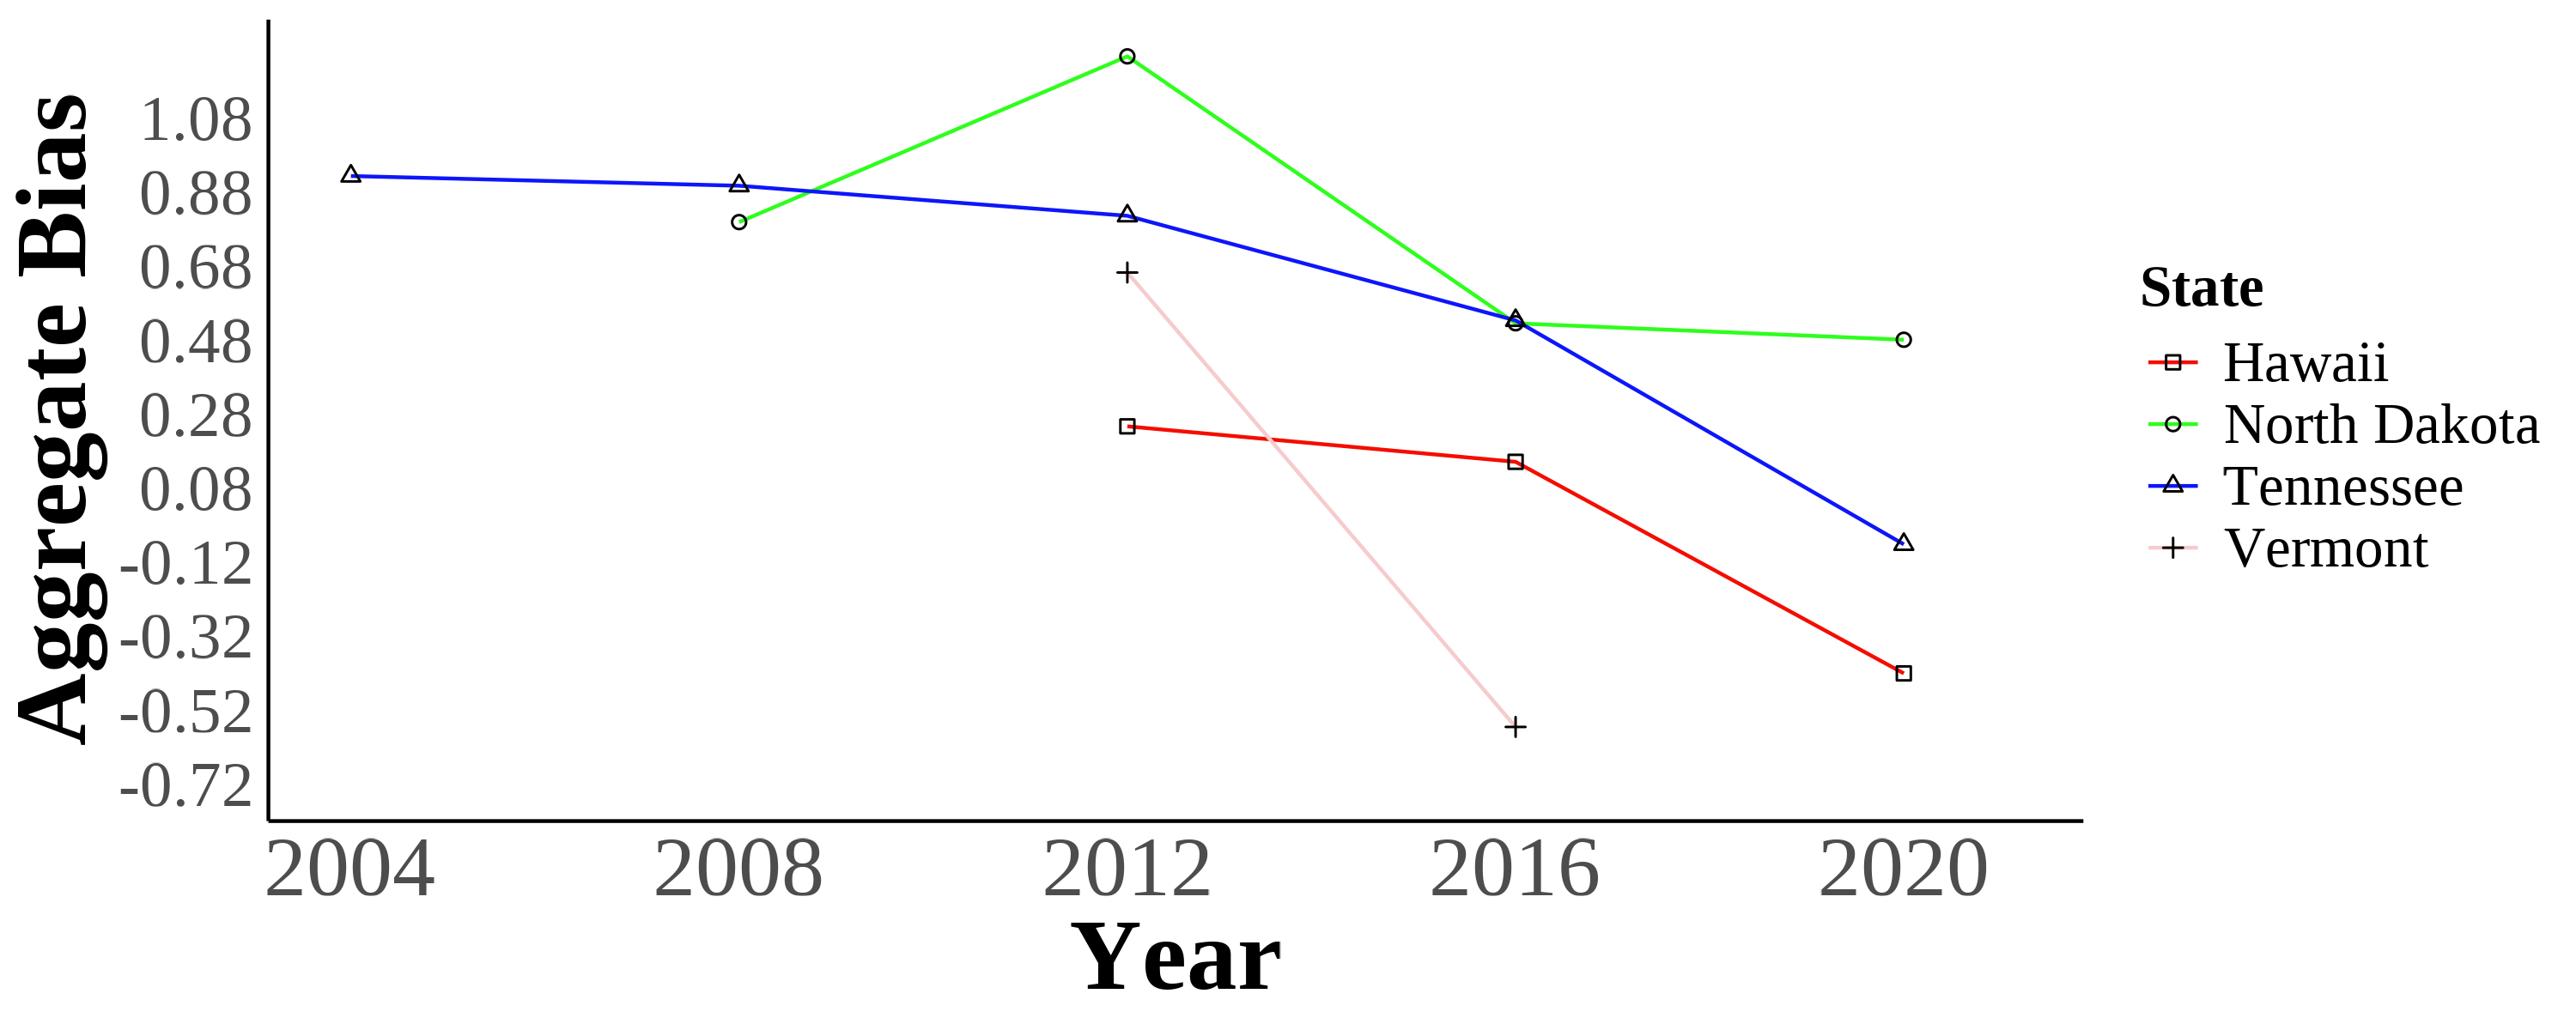
\includegraphics[width=.9\linewidth]{Bias_twostates.png} 
\label{fig:skiniat}
\end{subfigure}
% Second
\begin{subfigure}{.9\textwidth}
\caption{Self-reported Asian Identity Over Time}
\centering
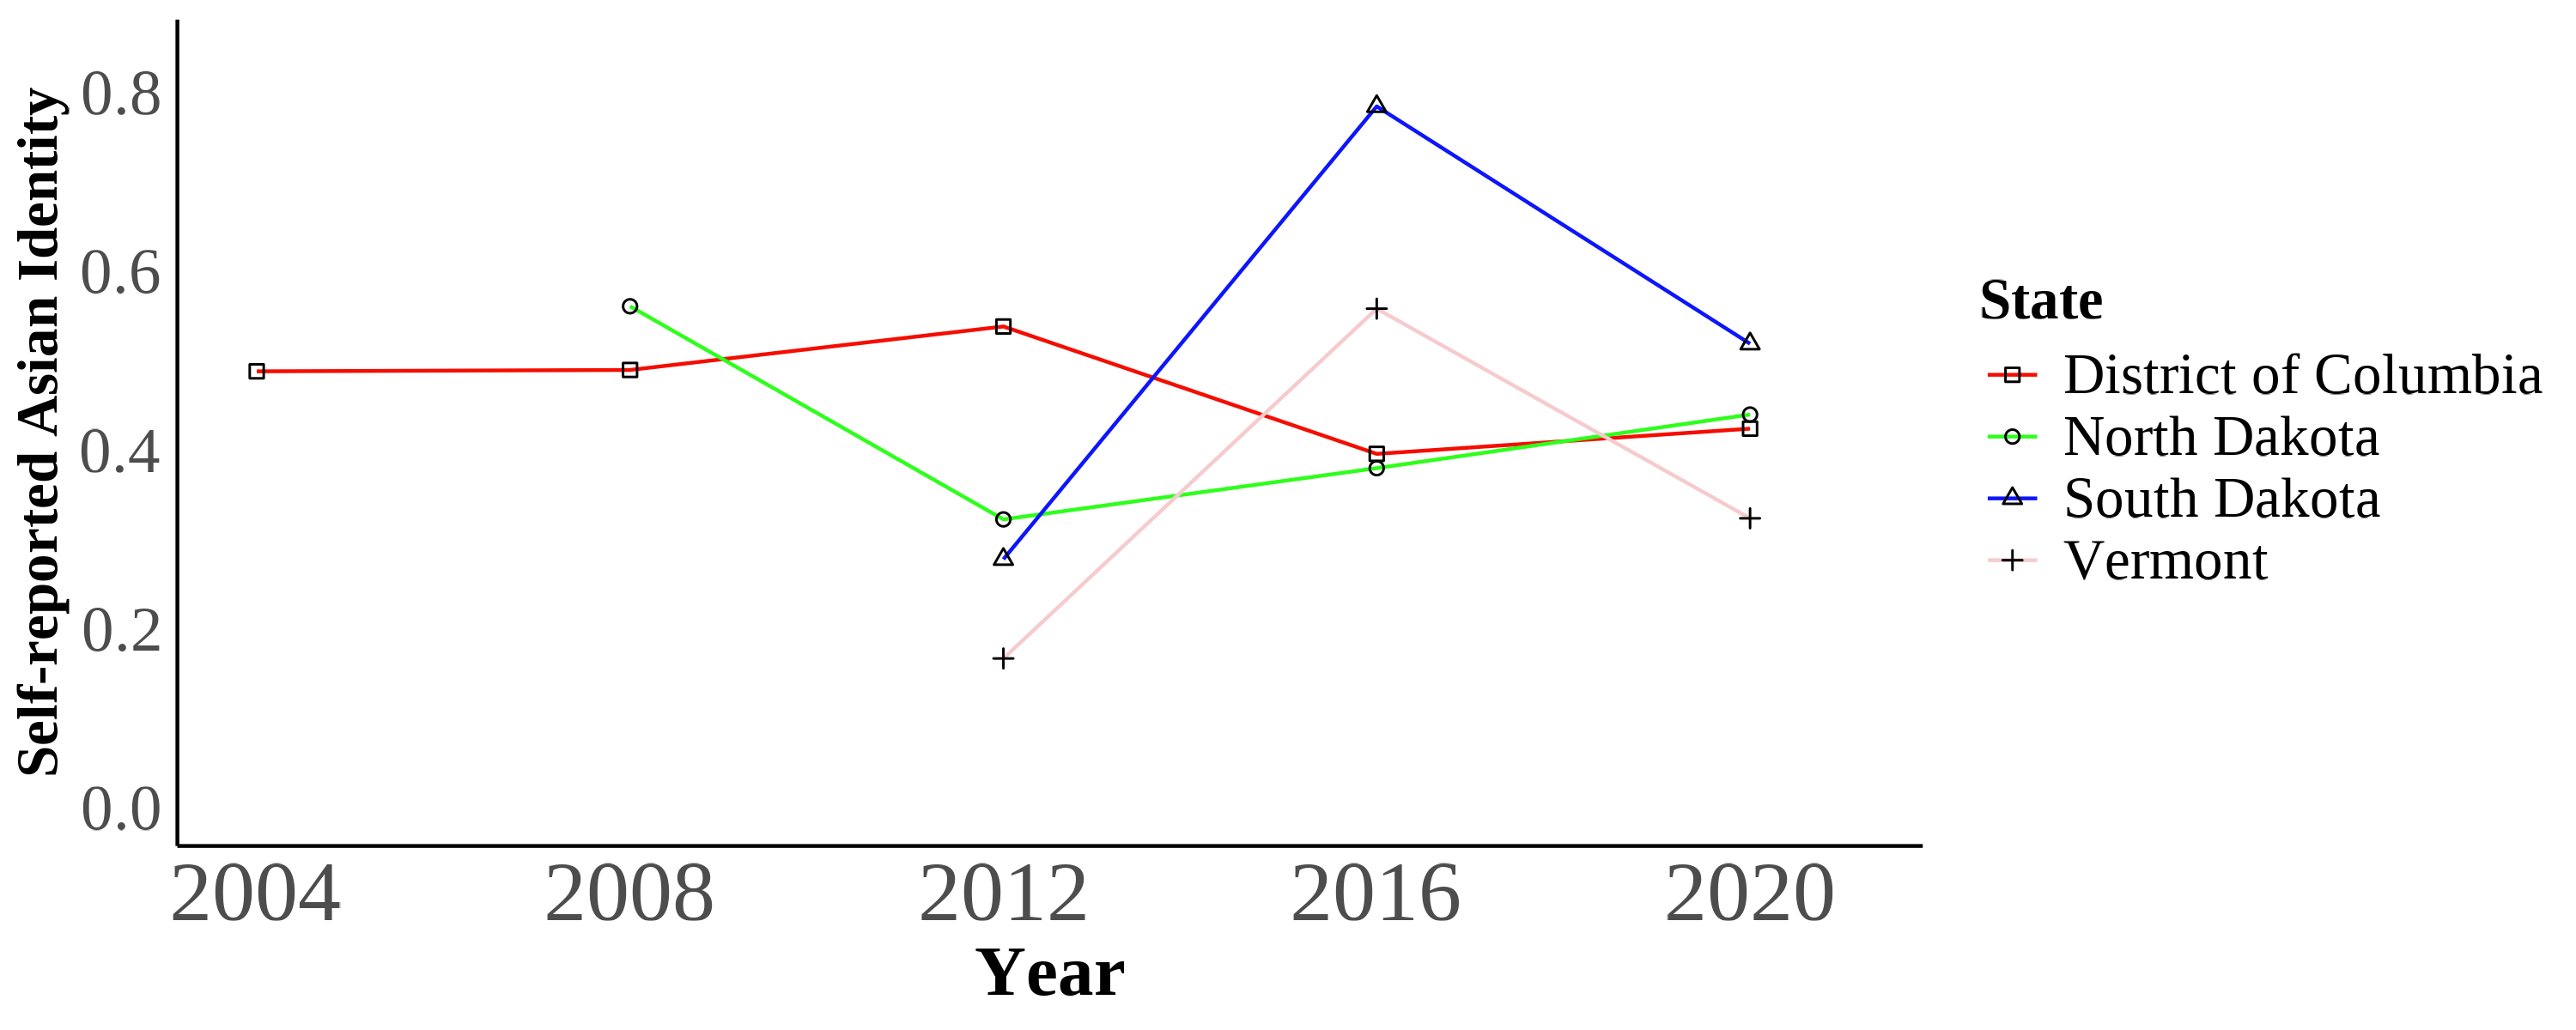
\includegraphics[width=.9\linewidth]{Bias_twostates-asian.png} 
\label{fig:Asian-twostates}
\end{subfigure}
\caption*{\footnotesize{These two panels show the trends in bias (panel a) and self-reported Asian identity among Asian immigrants (panel b) of the least and most biased places in the data. The District of Colombia is the least biased geographical area, and North Dakota is the most biased. The bias units are in standard deviations. Self-reported Asian identity is among first, second, and third-generation Asian immigrants aged 17 and younger still living in intact families.\\
Bias data is from the 2004--2021 Harvard's Project Implicit Association Test scores, American National Election Studies (ANES), and state-level hate crimes against Asians. Identity data is from the 2004--2021 Current Population Survey (CPS).}}
\end{figure}
\end{center}


\pagebreak
\newpage

\begin{center}
\begin{figure}[H]
\caption{Maps of State-level Association Test Bias Over Time Measure with Census Division Regional Boundaries}
\label{fig:skiniat-maps}
% first
\begin{subfigure}{.45\textwidth}
\caption{State-level Bias in 2004}
\centering
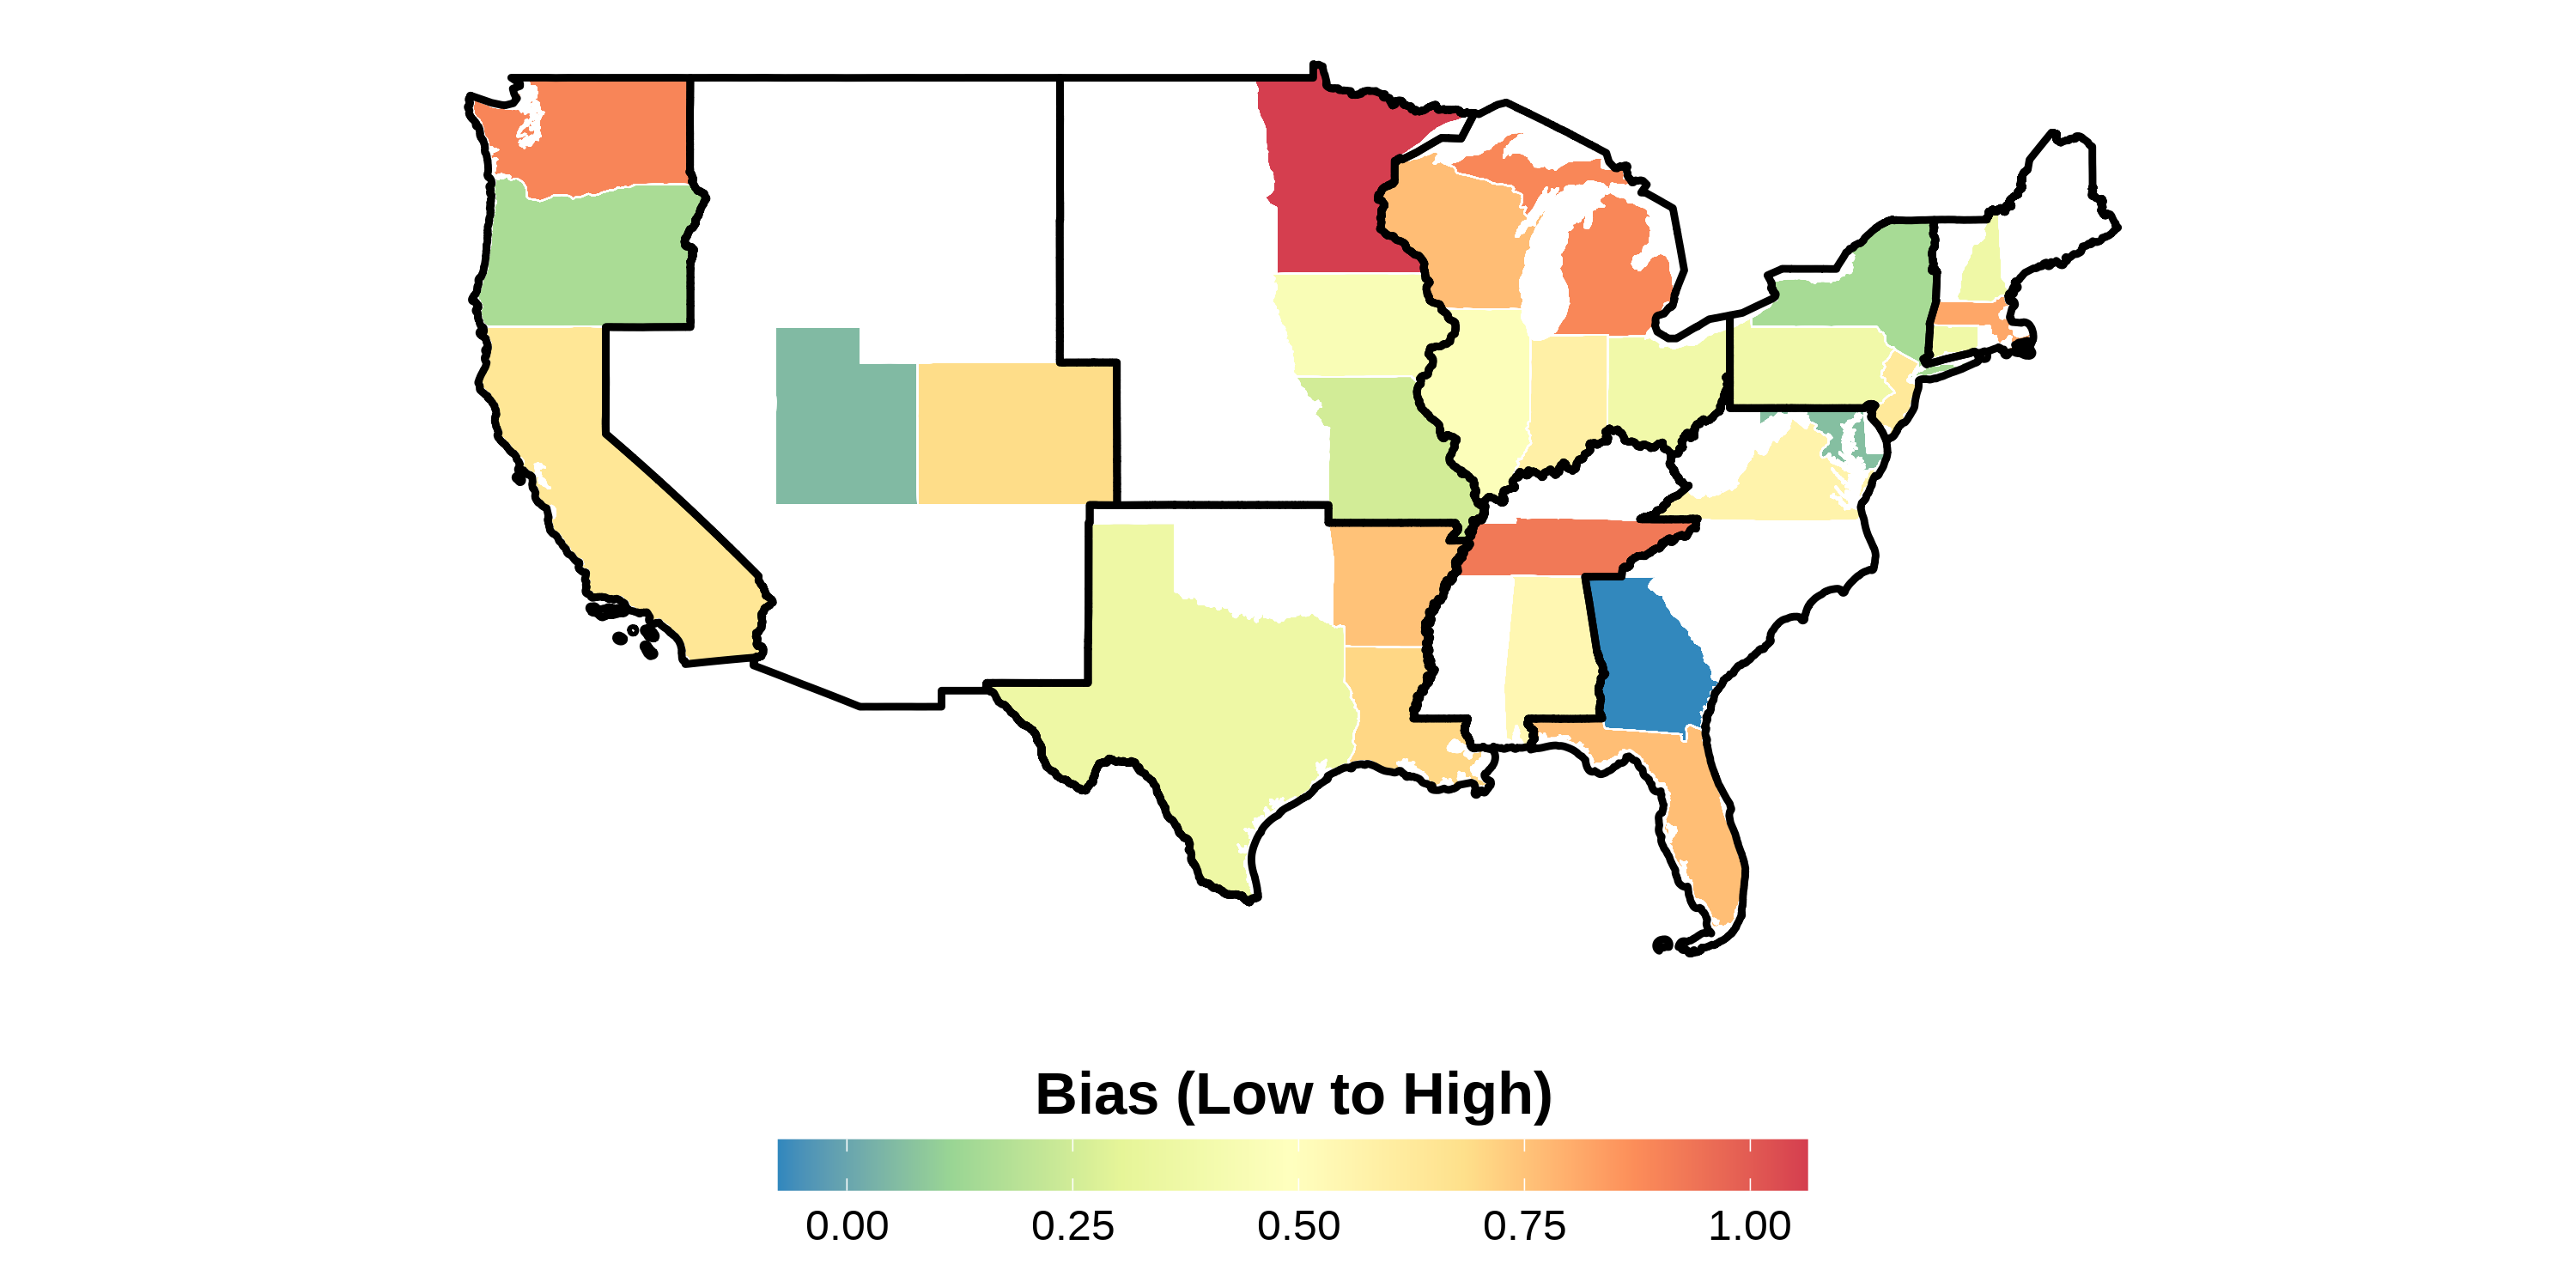
\includegraphics[width=0.9\linewidth]{2004skinmap.png} 
\label{fig:skiniat-map-2004}
\end{subfigure}
\hfill%
% Second
\begin{subfigure}{.45\textwidth}
\caption{State-level Bias in 2008}
\centering
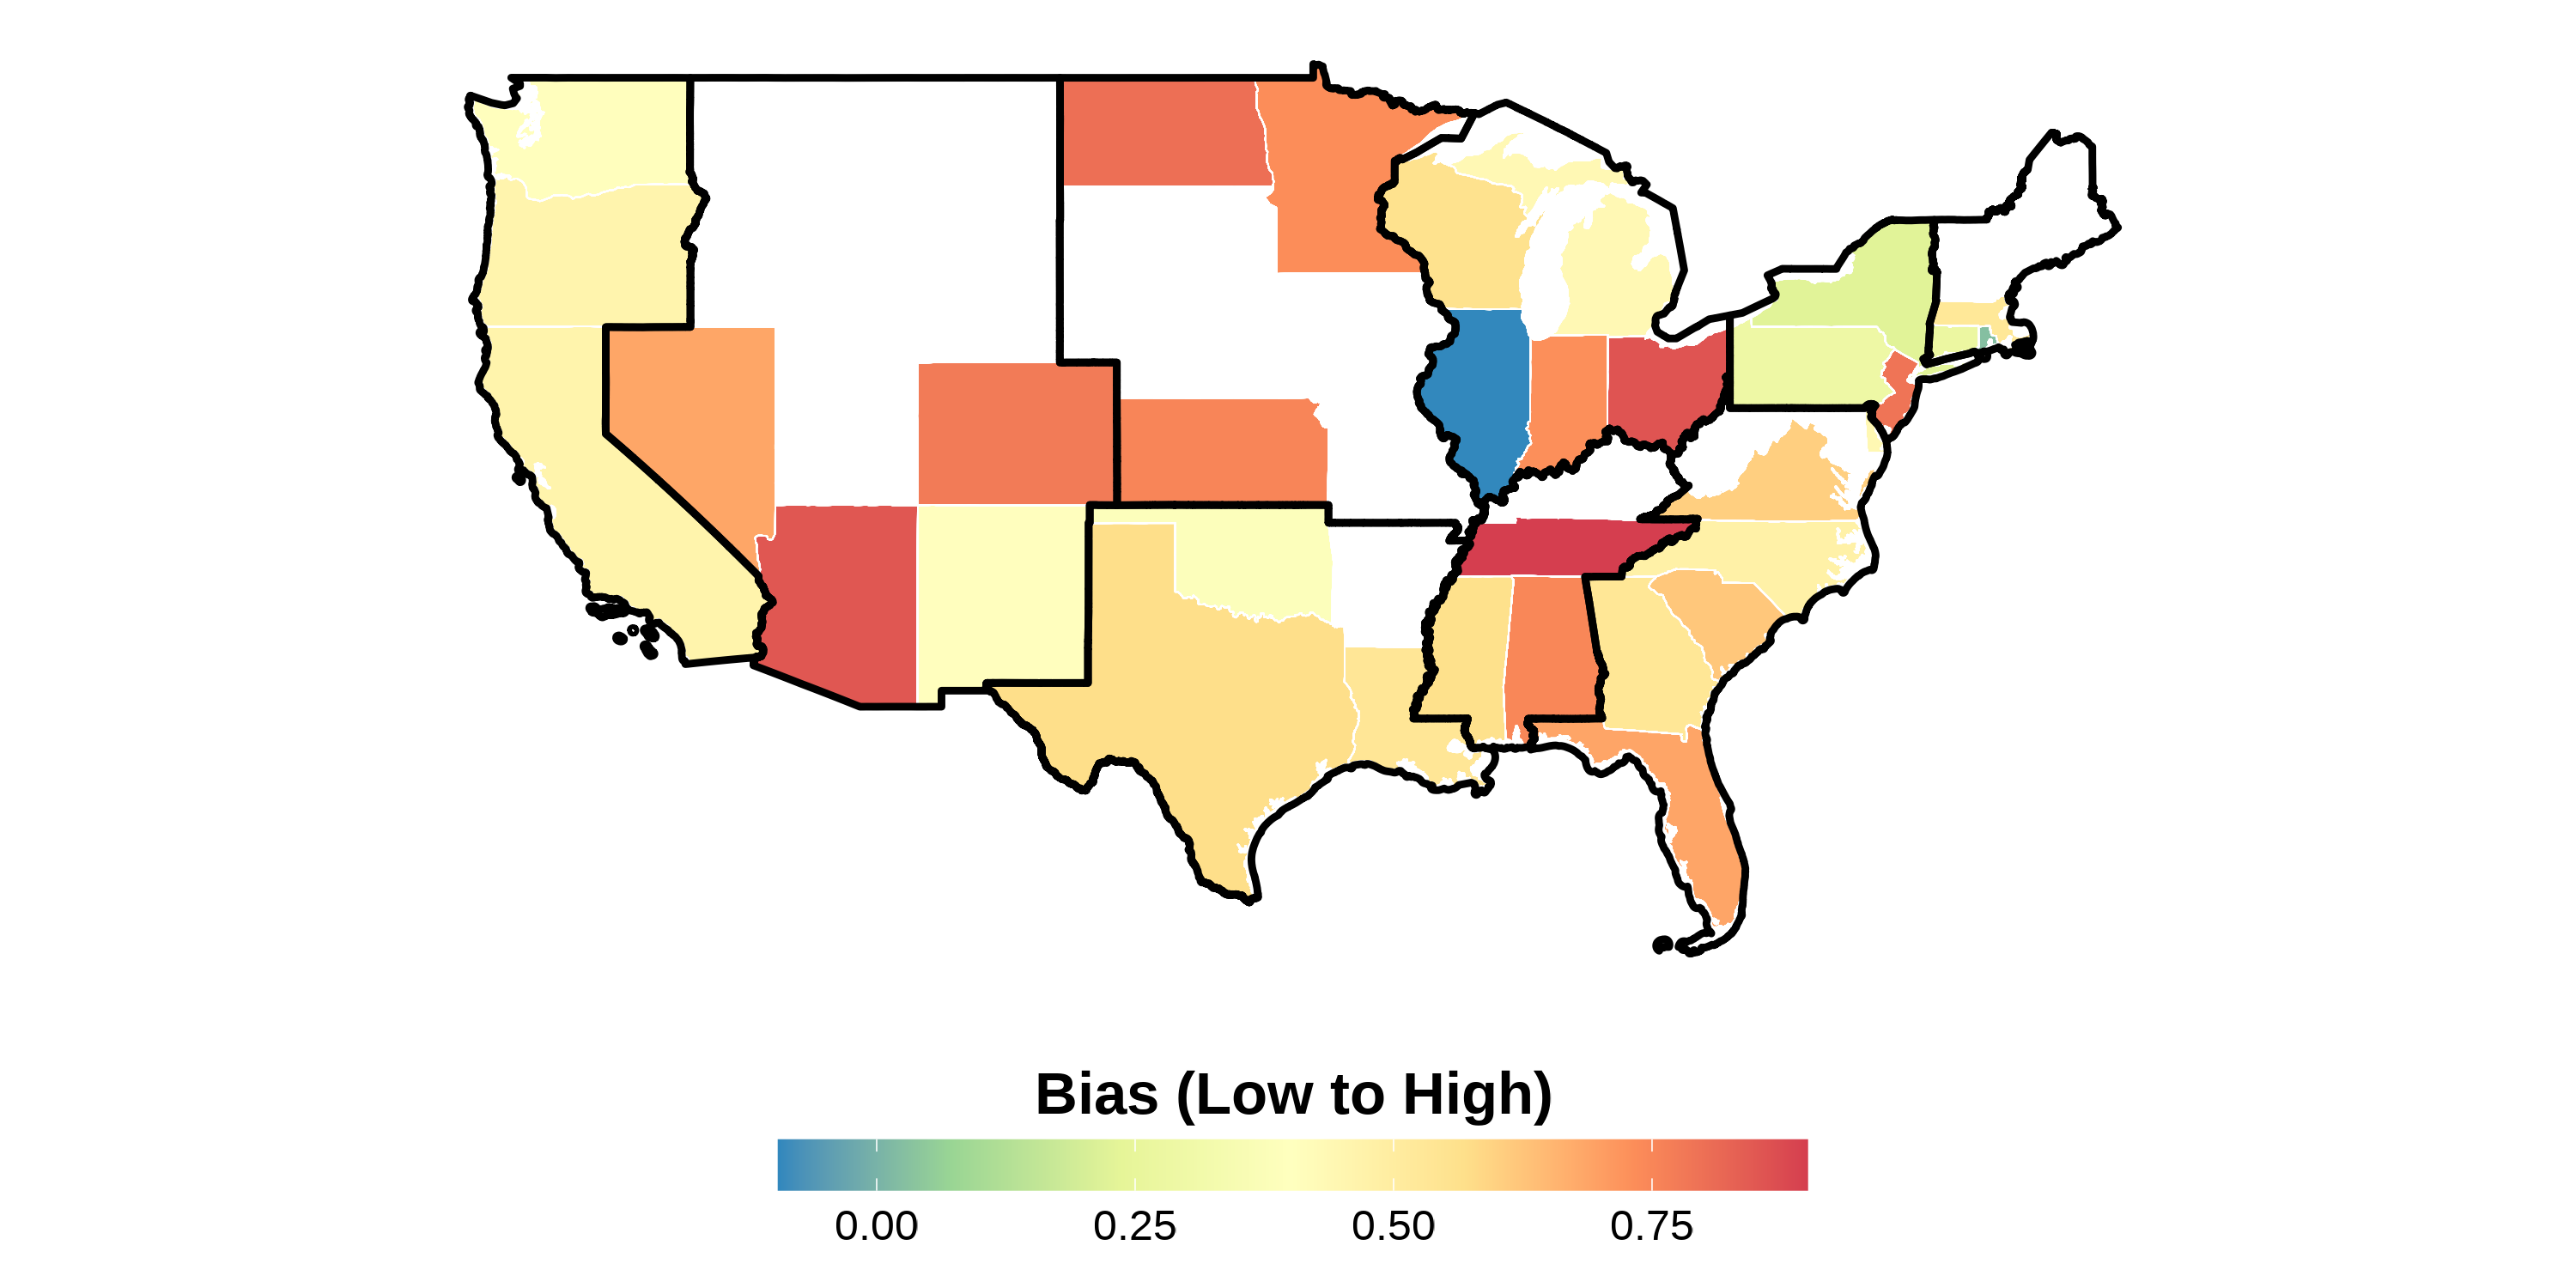
\includegraphics[width=0.9\linewidth]{2008skinmap.png} 
\label{fig:skiniat-map-2006}
\end{subfigure}
\hfill%
% third
\begin{subfigure}{.45\textwidth}
\caption{State-level Bias in 2012}
\centering
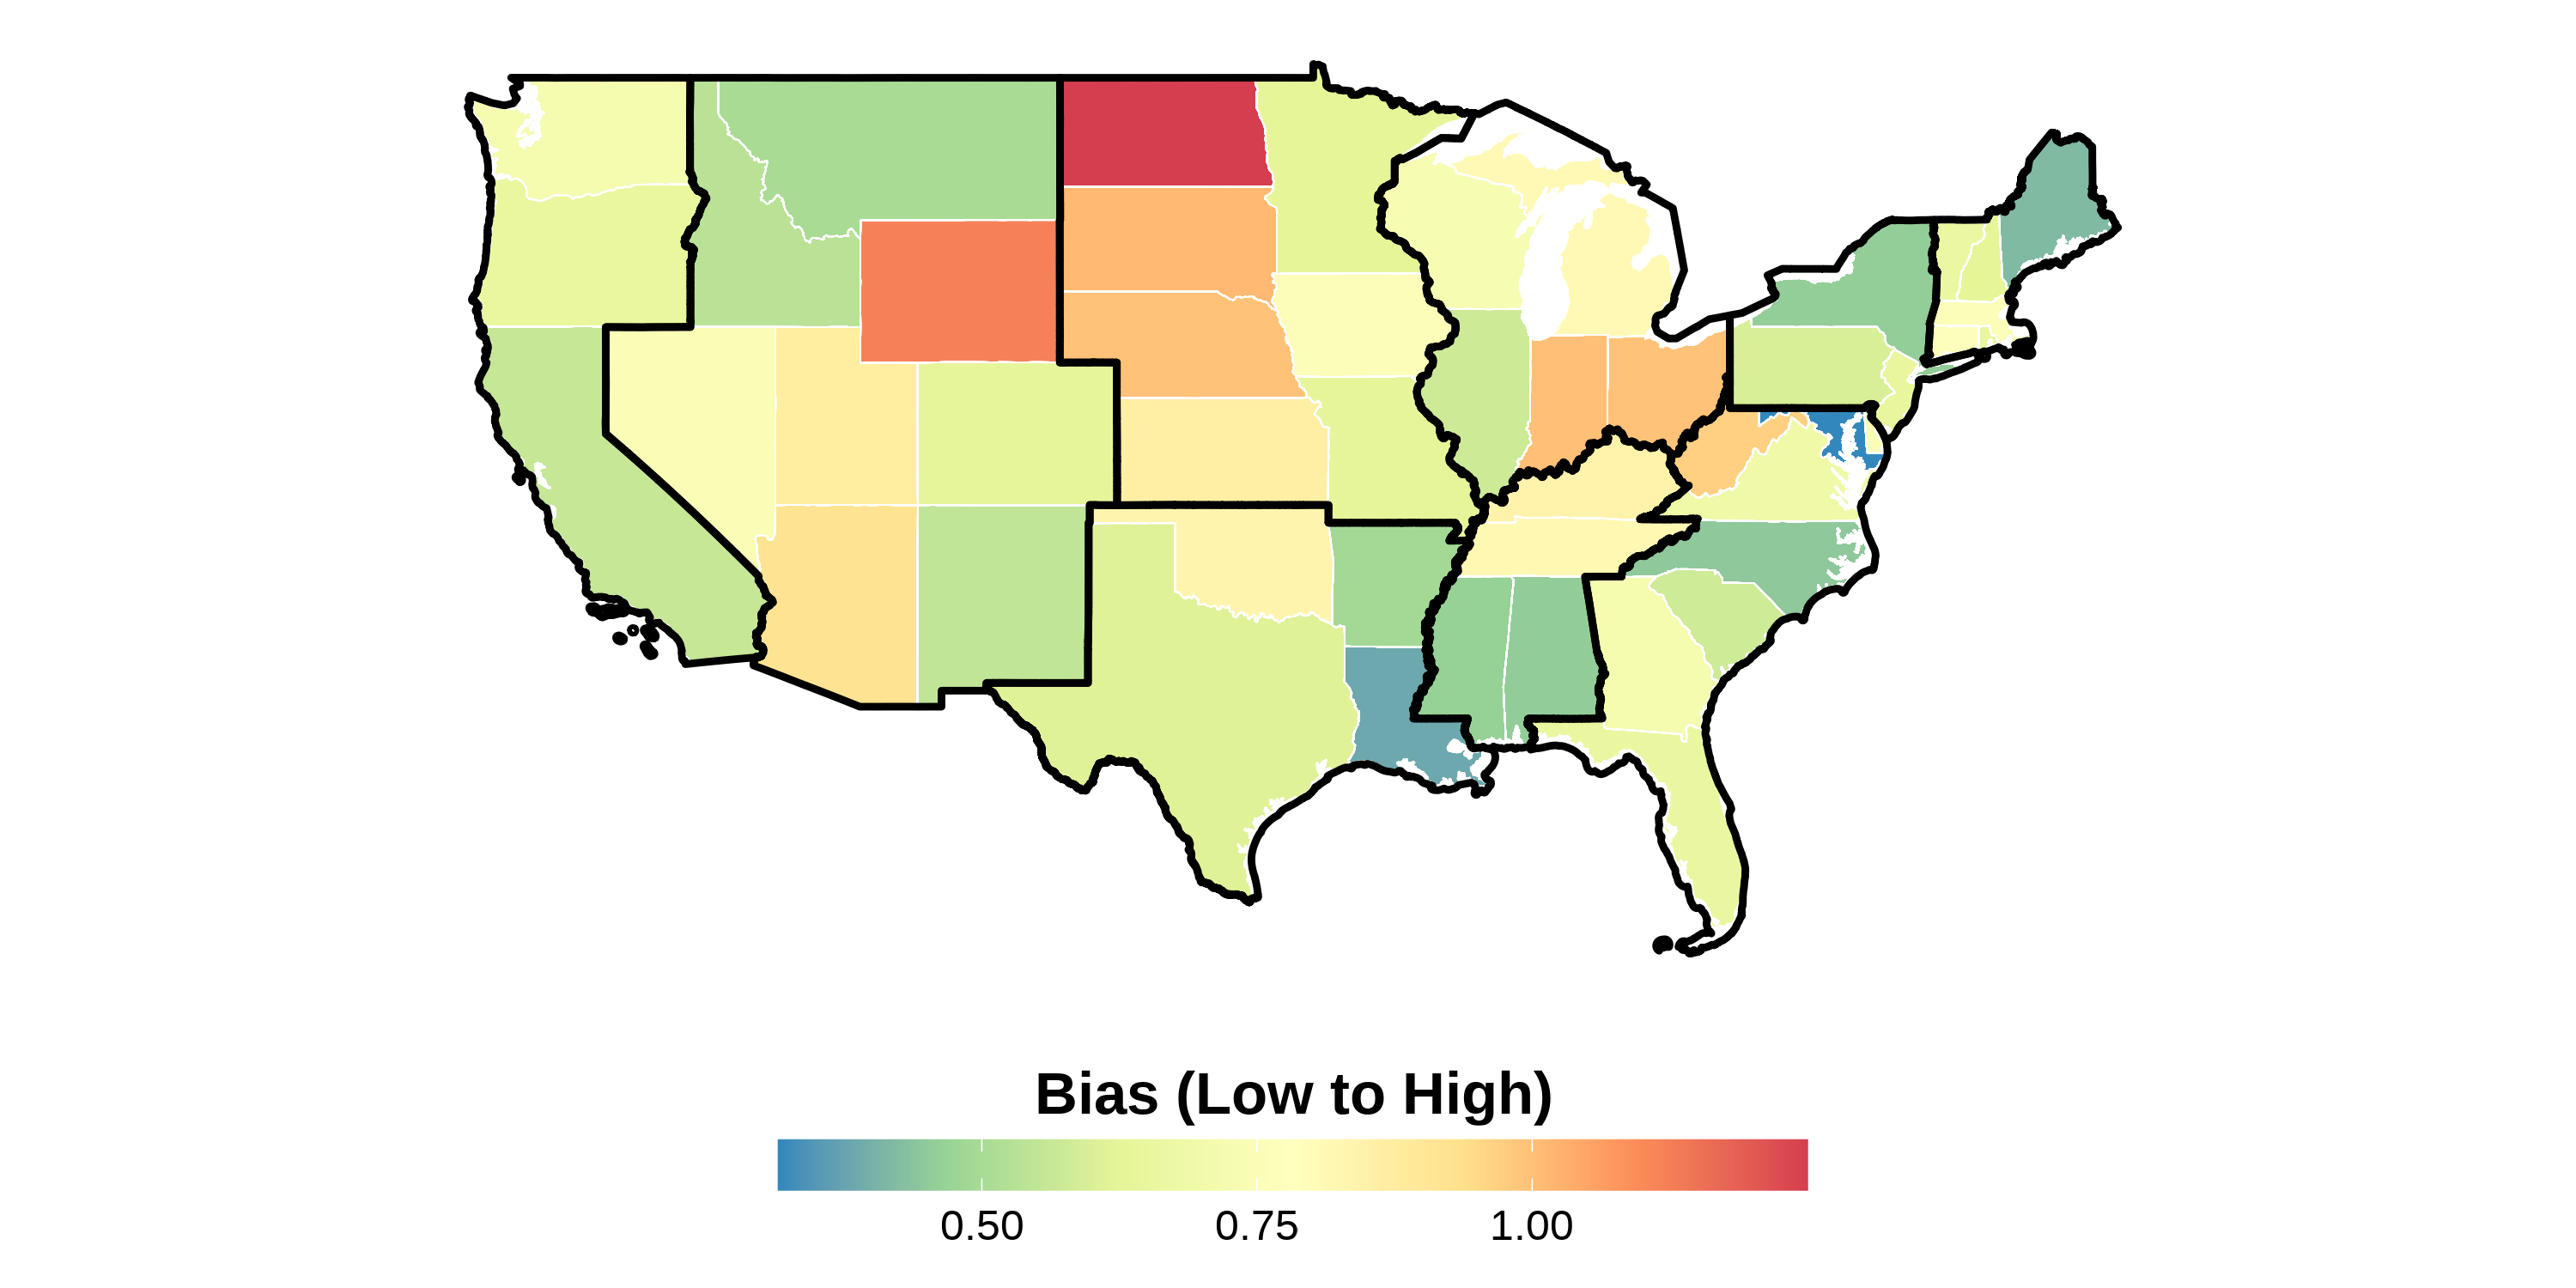
\includegraphics[width=0.9\linewidth]{2012skinmap.png} 
\label{fig:skiniat-map-2008}
\end{subfigure}
\hfill%
% fourth
\begin{subfigure}{.45\textwidth}
\caption{State-level Bias in 2016}
\centering
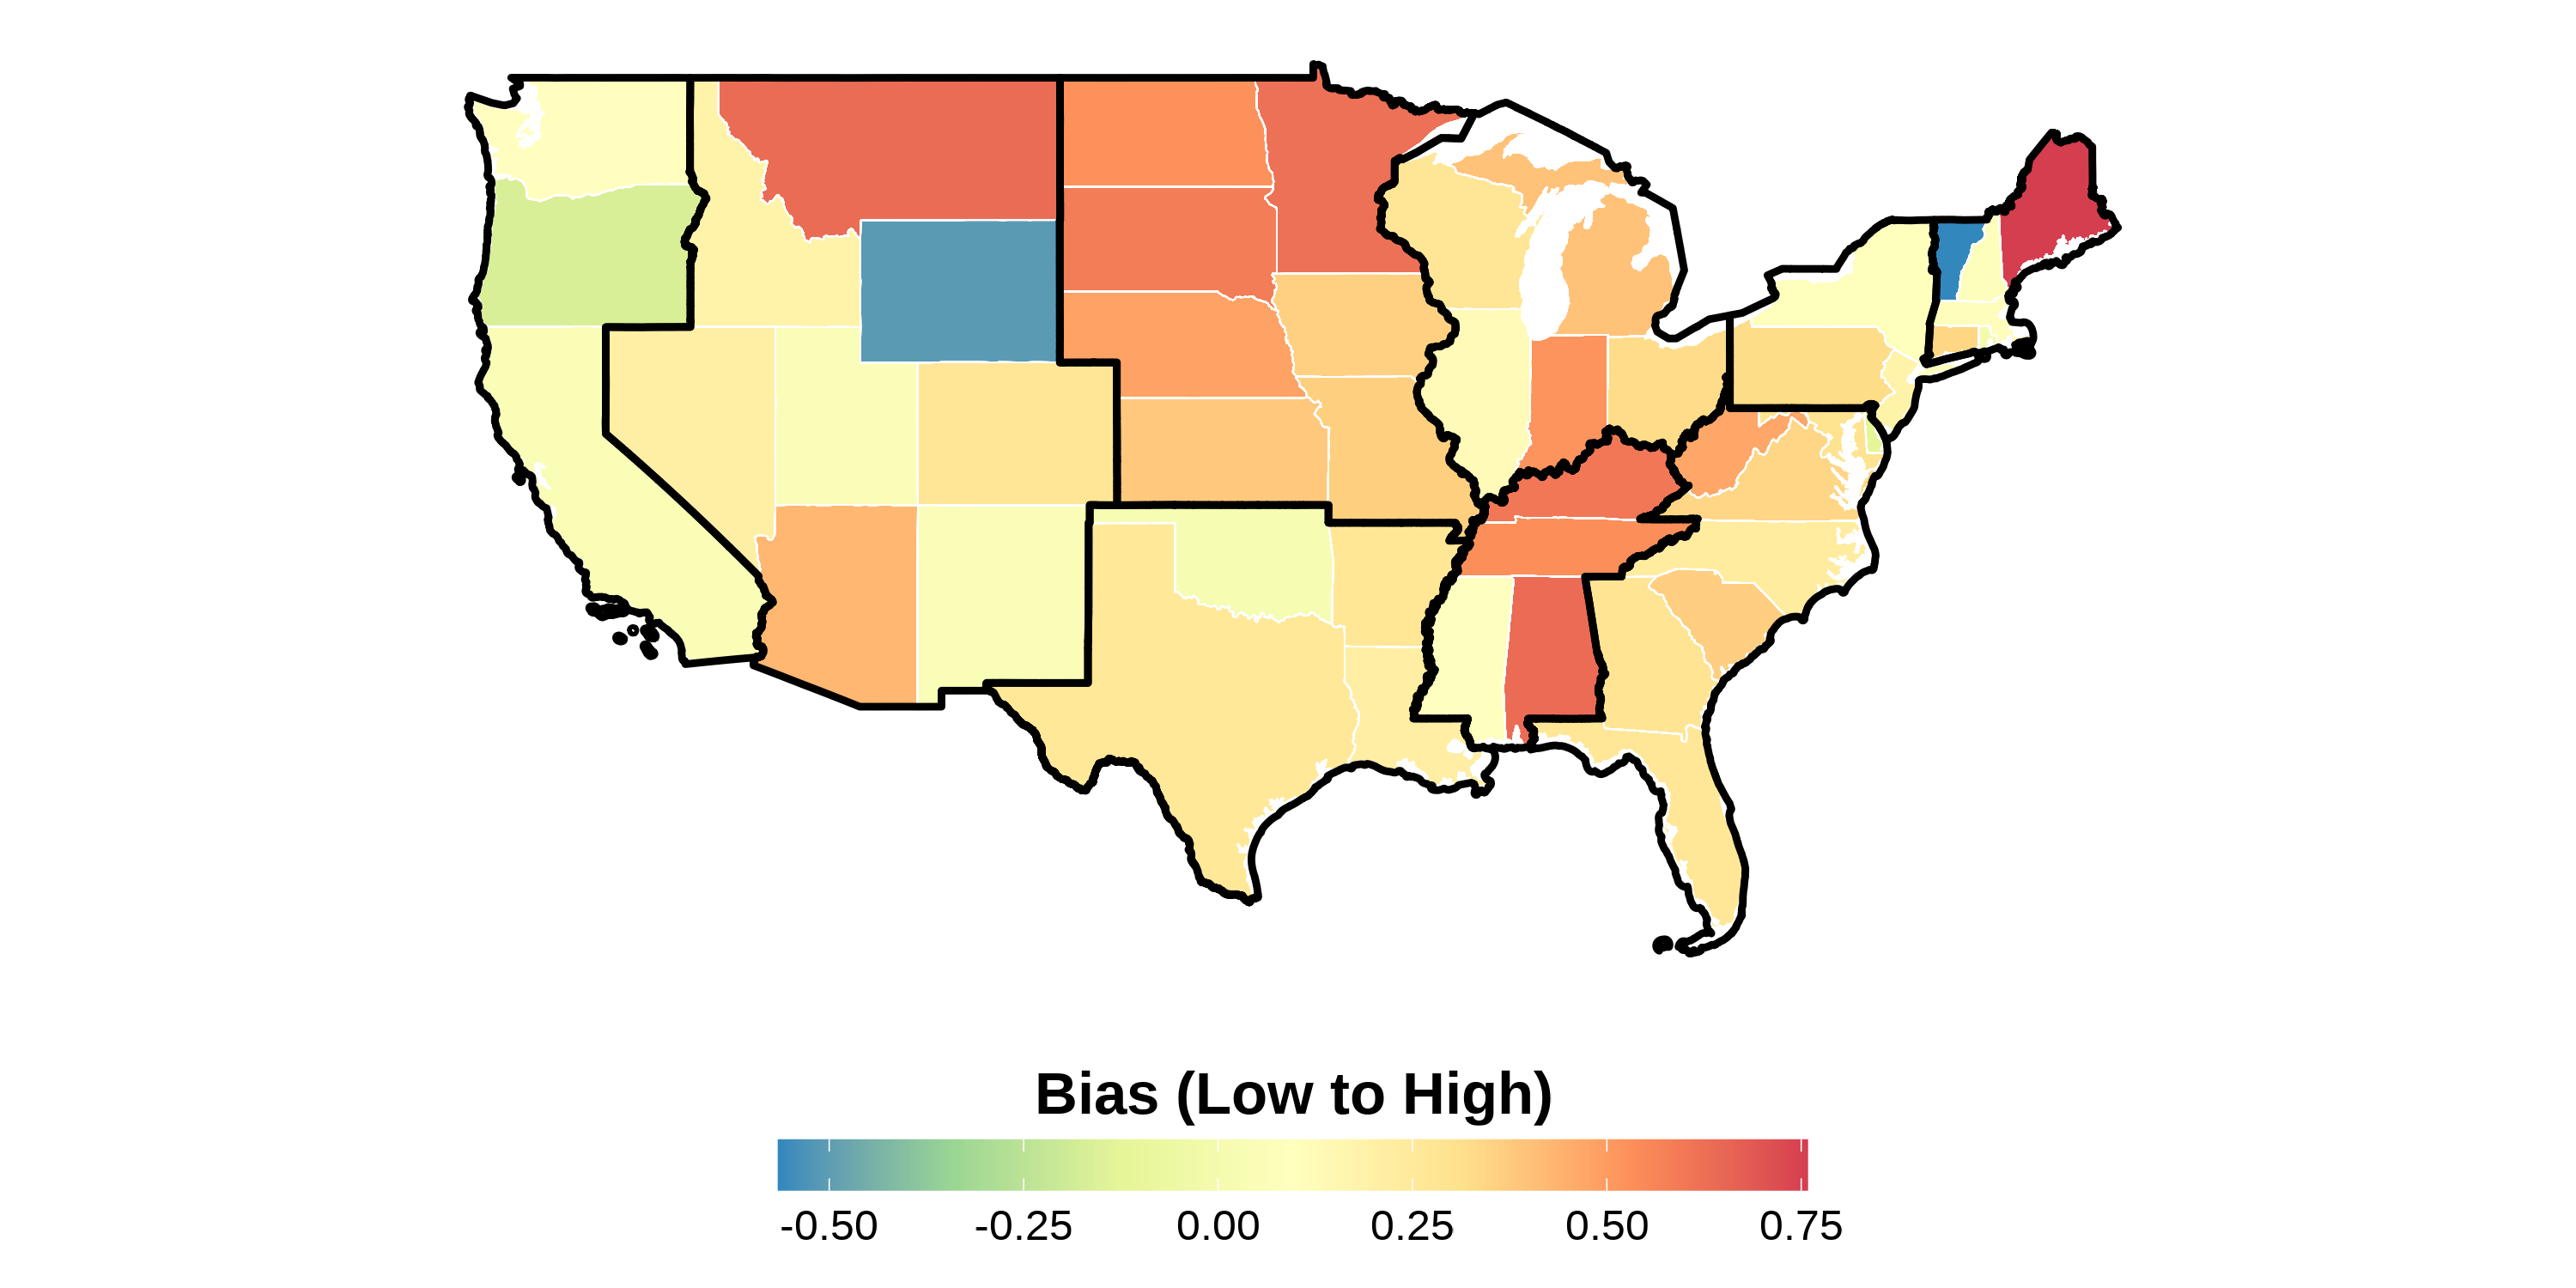
\includegraphics[width=0.9\linewidth]{2016skinmap.png} 
\label{fig:skiniat-map-2010}
\end{subfigure}

\caption*{\footnotesize{This figure shows the state-level bias index in different years in the sample. The bias units are in standard deviations and ranges from low to high bias. Bias index is constructed following \textcite{lubotskyInterpretationRegressionsMultiple2006}. The data is from the 2004--2021 Harvard's Project Implicit Association Test scores, American National Election Studies (ANES), and state-level hate crimes against Asians. Each panel presents state-level bias during a certain year. The boundaries in black represent the different Census divisions in the United States. Notice how there is a variation across states within a region.}}
\end{figure}
\end{center}

\newpage
\pagebreak

\begin{center}
\begin{figure}[H]
\caption{Maps of State-level Bias 2004--2021 Measure with Census Division Regional Boundaries}
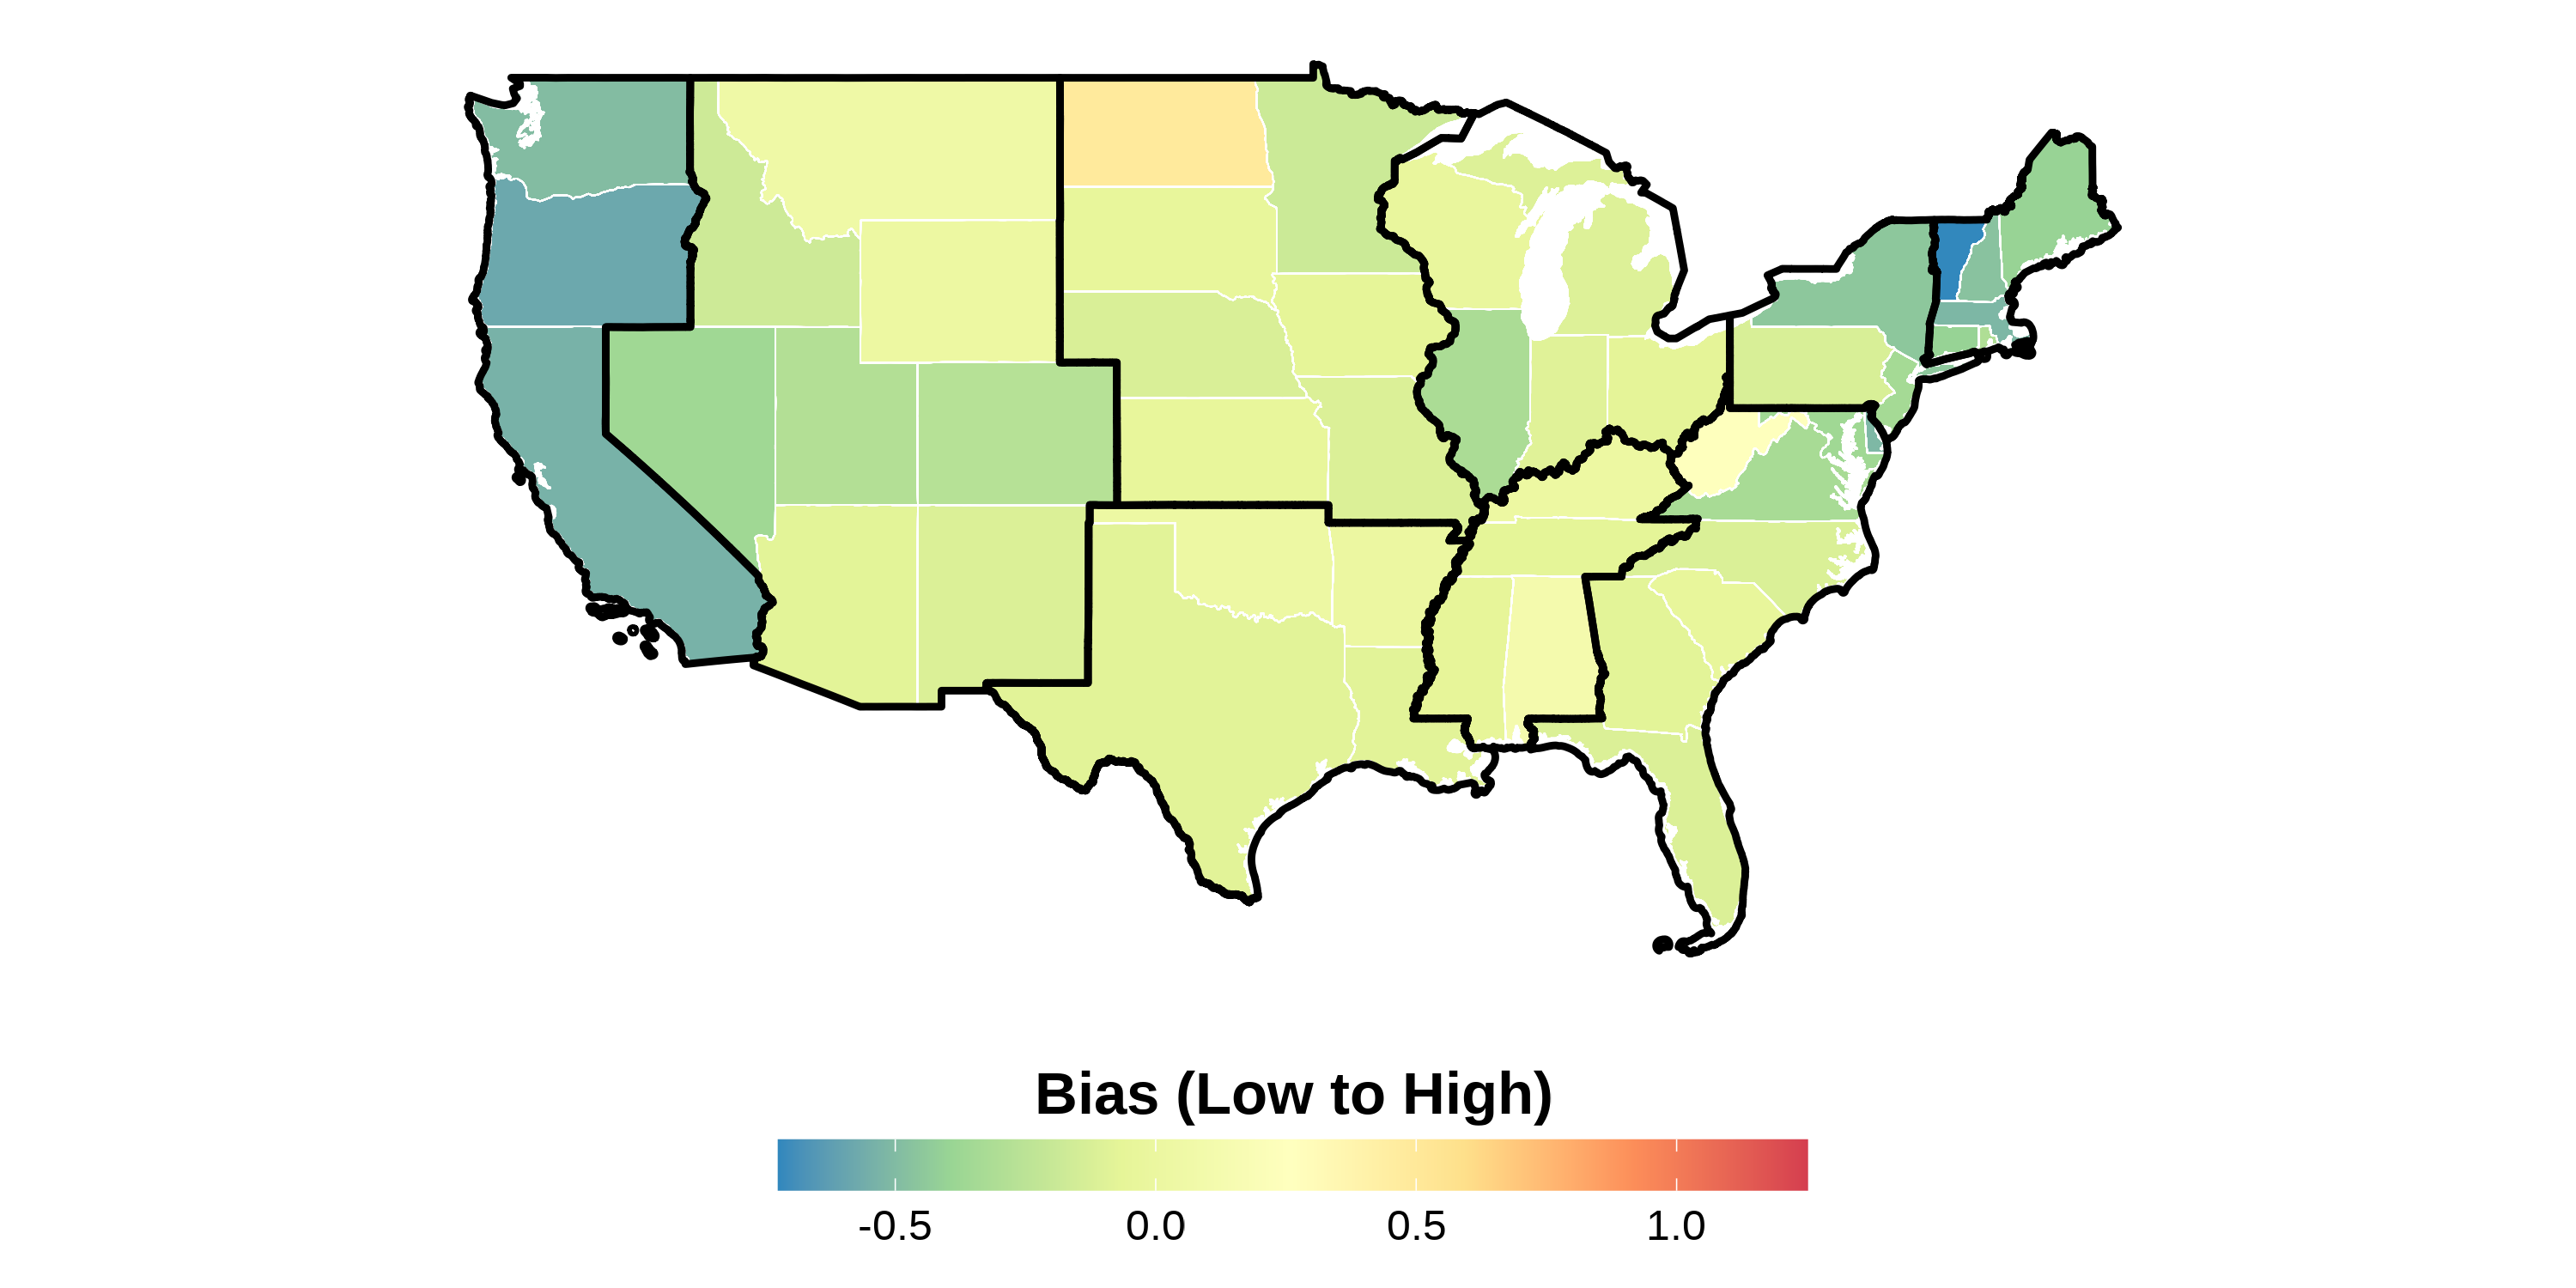
\includegraphics[width=\textwidth]{Average_Skinmap.png} 
\label{fig:iat-map-all}
\caption*{\footnotesize{This figure shows the state-level bias index in the sample from 2004 to 2021. The bias units are in standard deviations and ranges from low to high bias. Bias index is constructed following \textcite{lubotskyInterpretationRegressionsMultiple2006}. The data is from the 2004--2021 Harvard's Project Implicit Association Test scores, American National Election Studies (ANES), and state-level hate crimes against Asians. The boundaries in black represent the different Census divisions in the United States. Notice how there is a variation across states within a region.}}
\end{figure}
\end{center}

\newpage
\pagebreak

\begin{center}
\begin{figure}[H]
\caption{Asian Racial Identity}
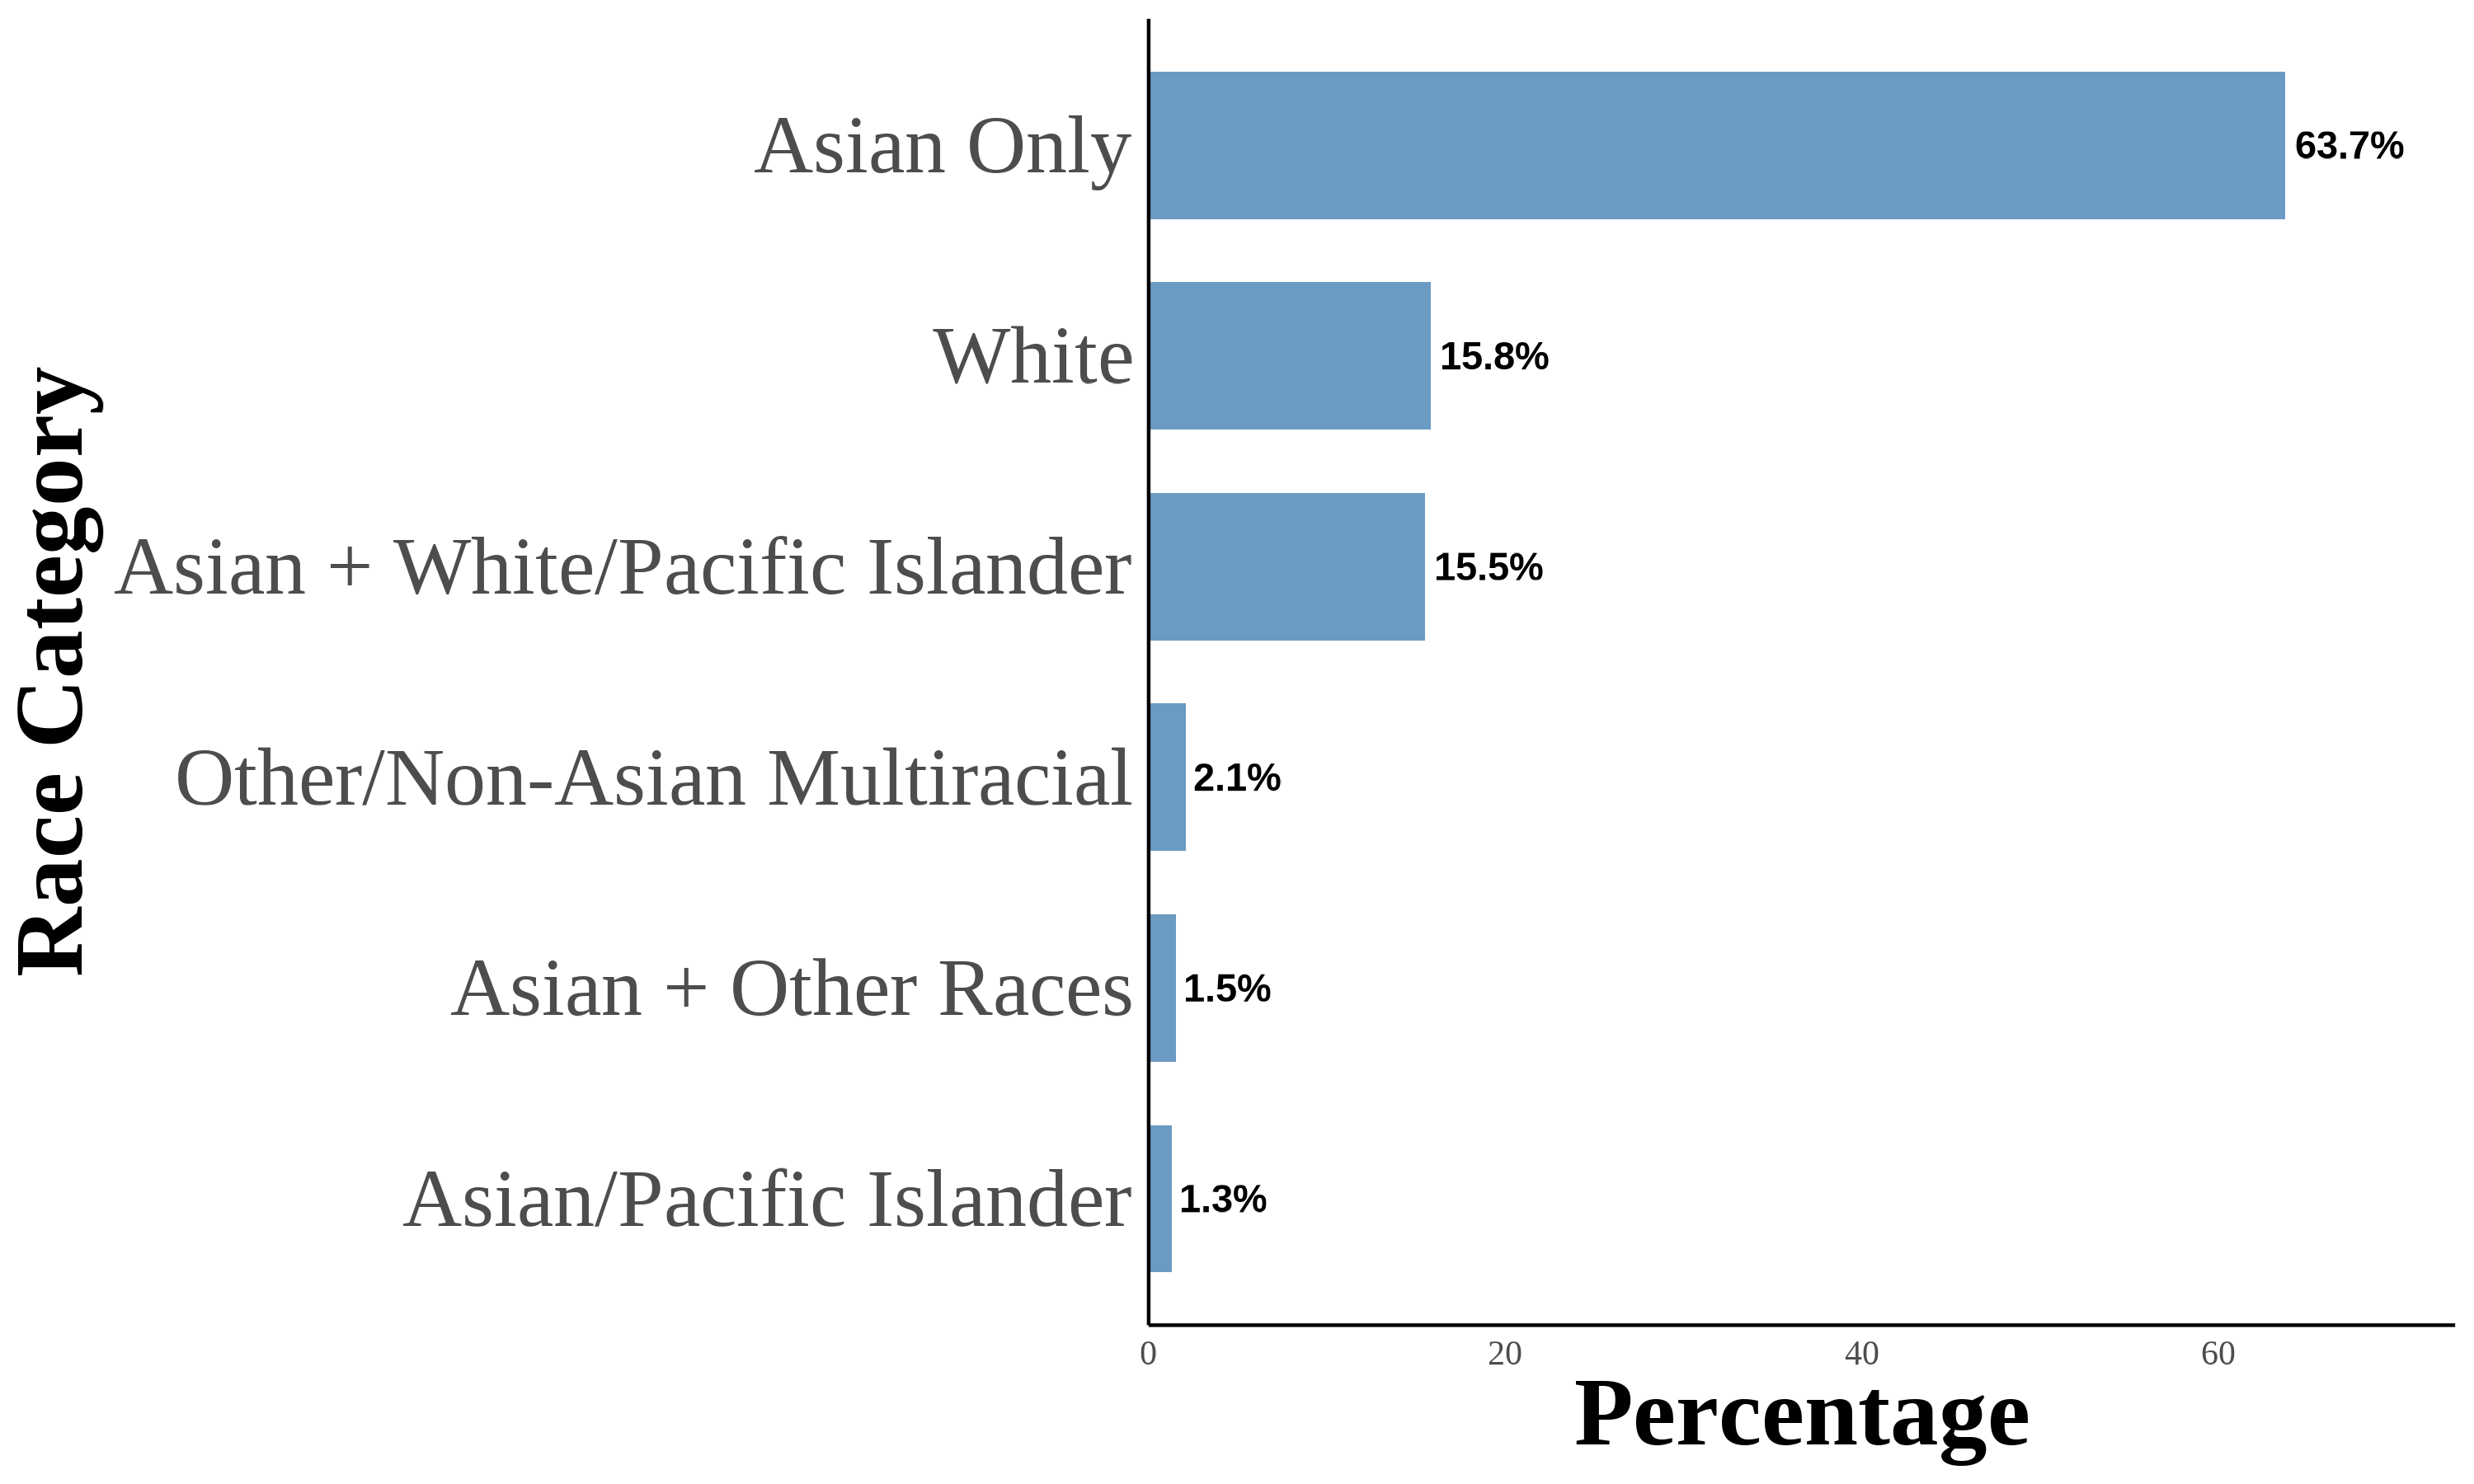
\includegraphics[width=\textwidth]{histogram_asian_american_race_aggregated.png} 
\label{fig:histogram-all}
\caption*{\footnotesize{This figure shows the distribution of Asian racial identity among respondents. 
The data is aggregated from the 2004--2021 Current Population Survey (CPS). 
The sample includes first-, second-, and third-generation objectively Asian Americans.
Following \textcite{antmanEthnicAttritionObserved2016,antmanEthnicAttritionAssimilation2020}, 
I utilize birthplace information for individuals, parents, and grandparents to create objective Asian ancestry indicators.
}}
\end{figure}
\end{center}

\newpage
\pagebreak

\begin{center}
\begin{figure}[H]
\caption{Asian Racial Identity: First Generation}
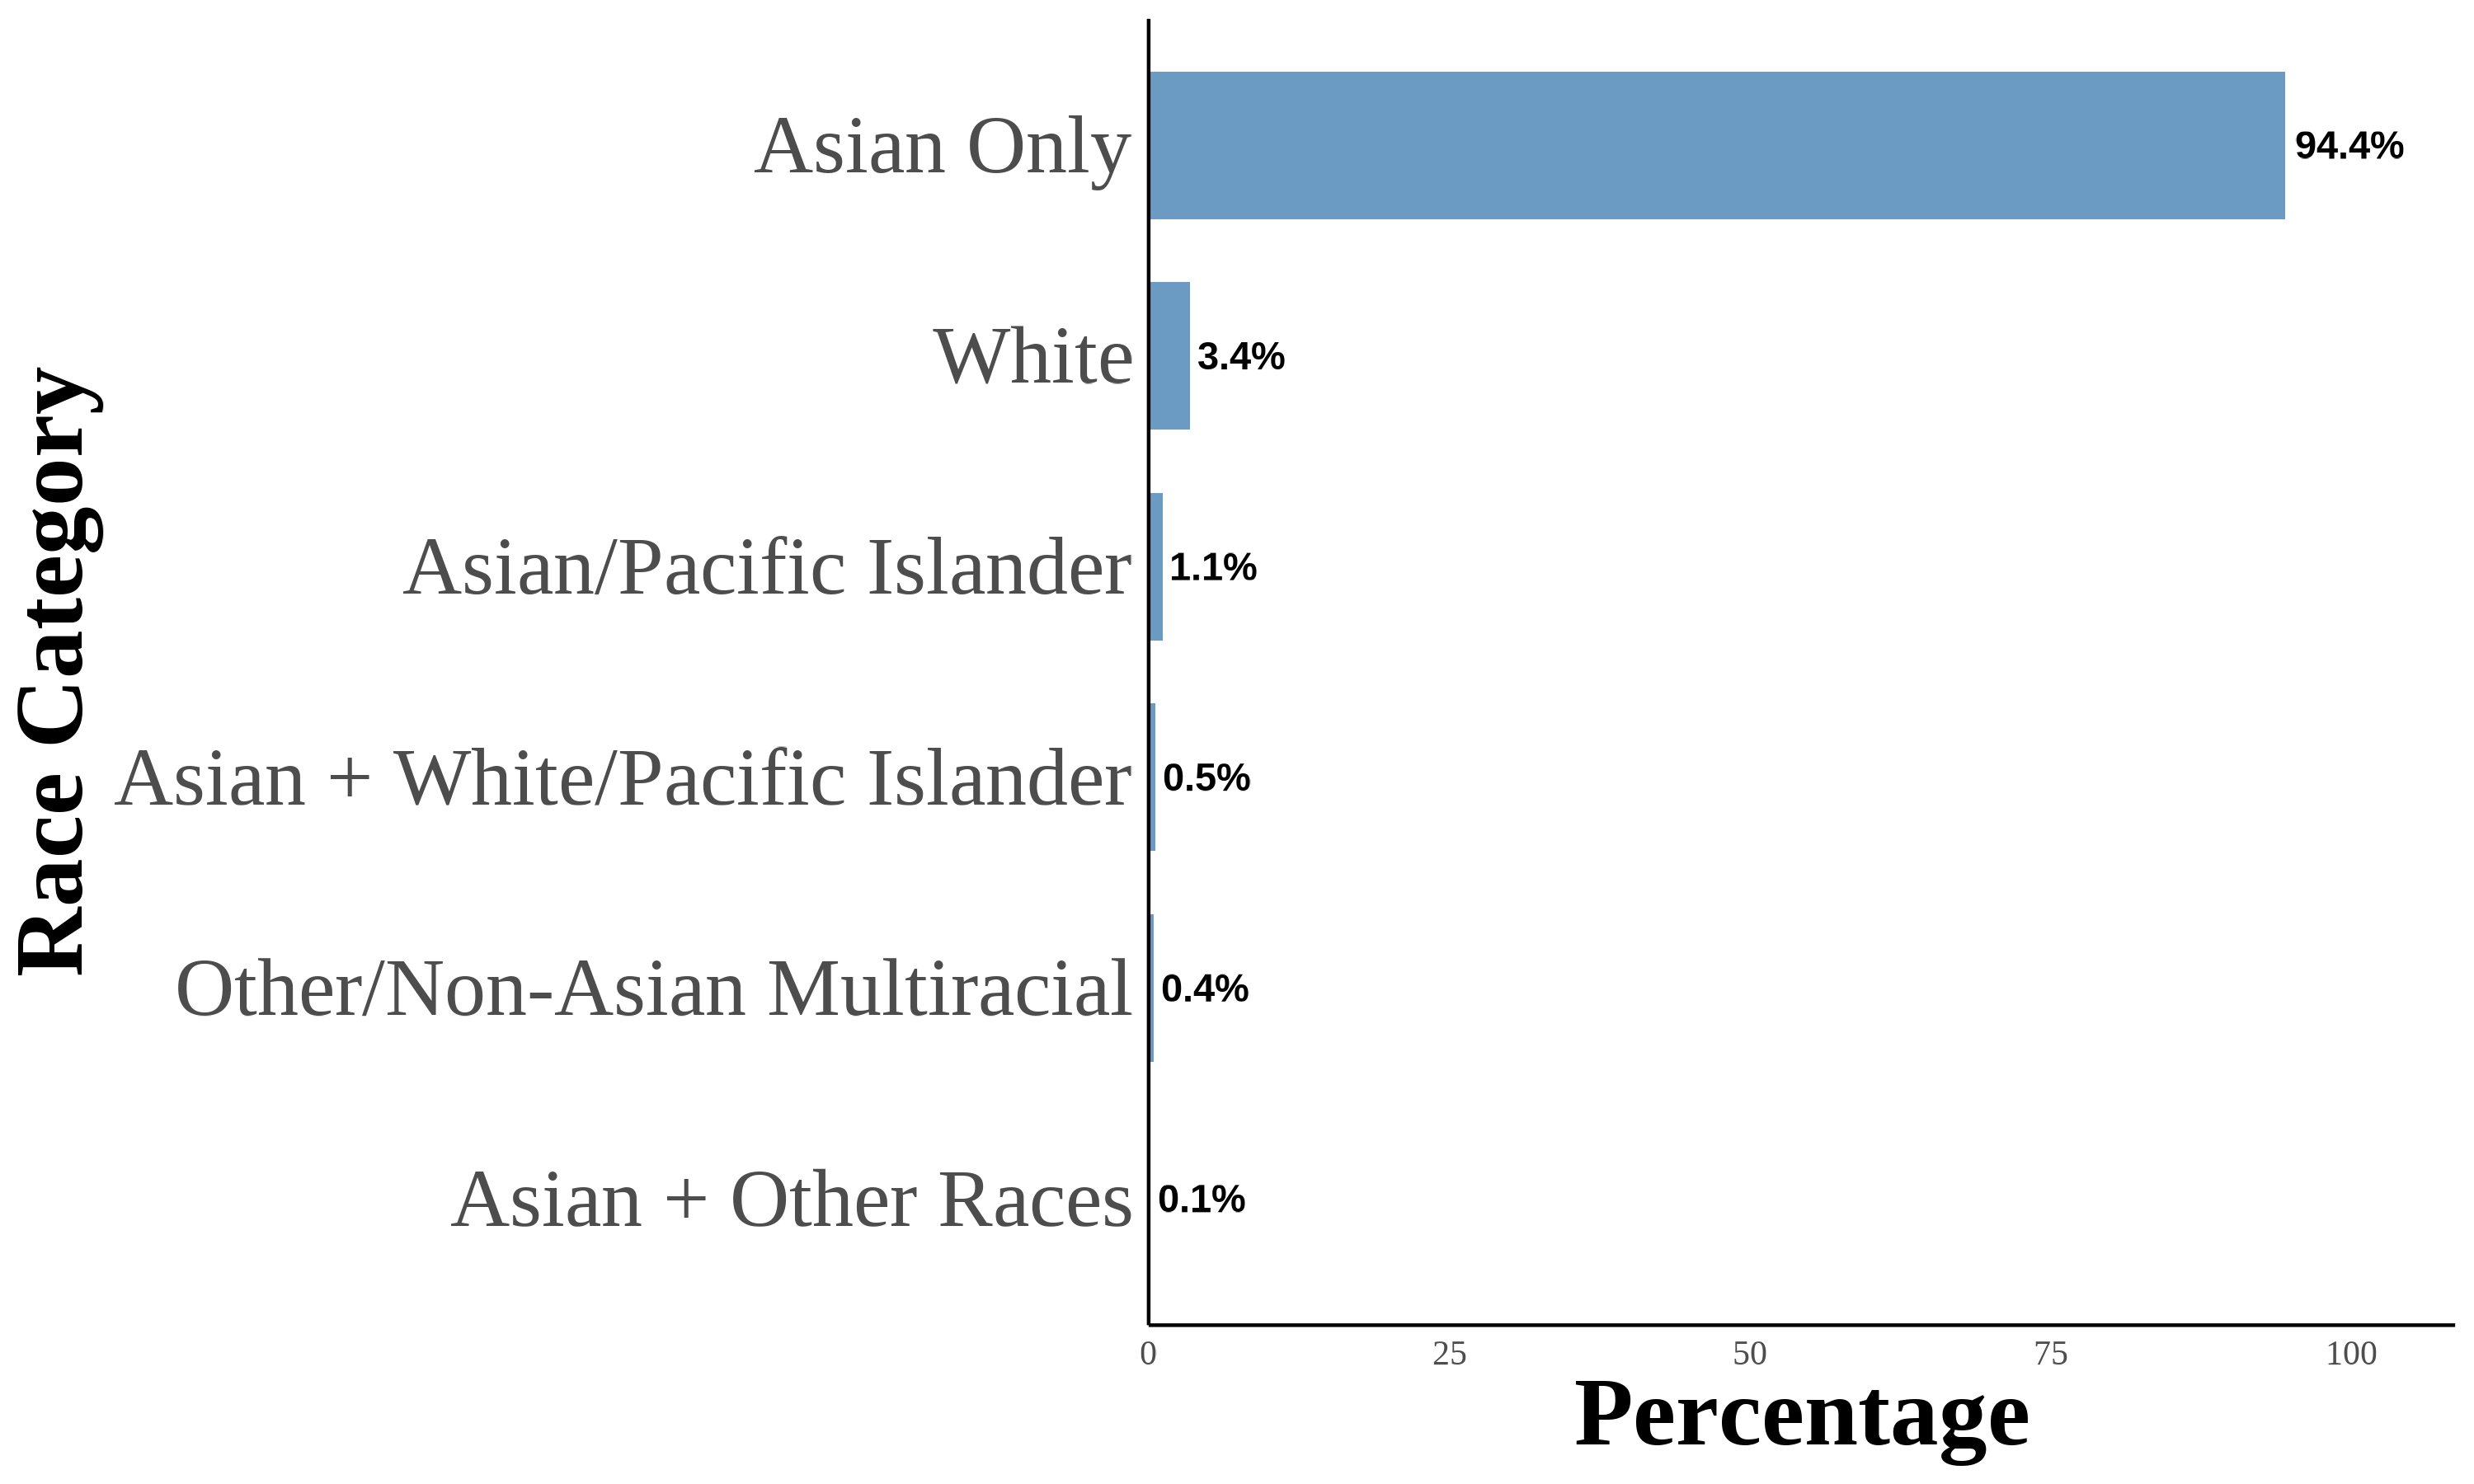
\includegraphics[width=\textwidth]{histogram_asian_american_race_firstgen.png} 
\label{fig:histogram-firstgen}
\caption*{\footnotesize{This figure shows the distribution of Asian racial identity among respondents. 
The data is aggregated from the 2004--2021 Current Population Survey (CPS). 
The sample includes first-generation objectively Asian Americans.
Following \textcite{antmanEthnicAttritionObserved2016,antmanEthnicAttritionAssimilation2020}, 
I utilize birthplace information for individuals, parents, and grandparents to create objective Asian ancestry indicators.
A first-generation Asian American is defined as an individual born in an Asian country and is not a US citizen born to US citizen parents abroad.
}}
\end{figure}
\end{center}


\pagebreak
\newpage

\begin{landscape}
\begin{figure}[!htb]
\centering
\caption{Asian Racial Identity: Second Generation}
\label{fig:histogram-secondgen}

% Top row
\begin{subfigure}{.48\textwidth}
\caption{All Second Generation}
\centering
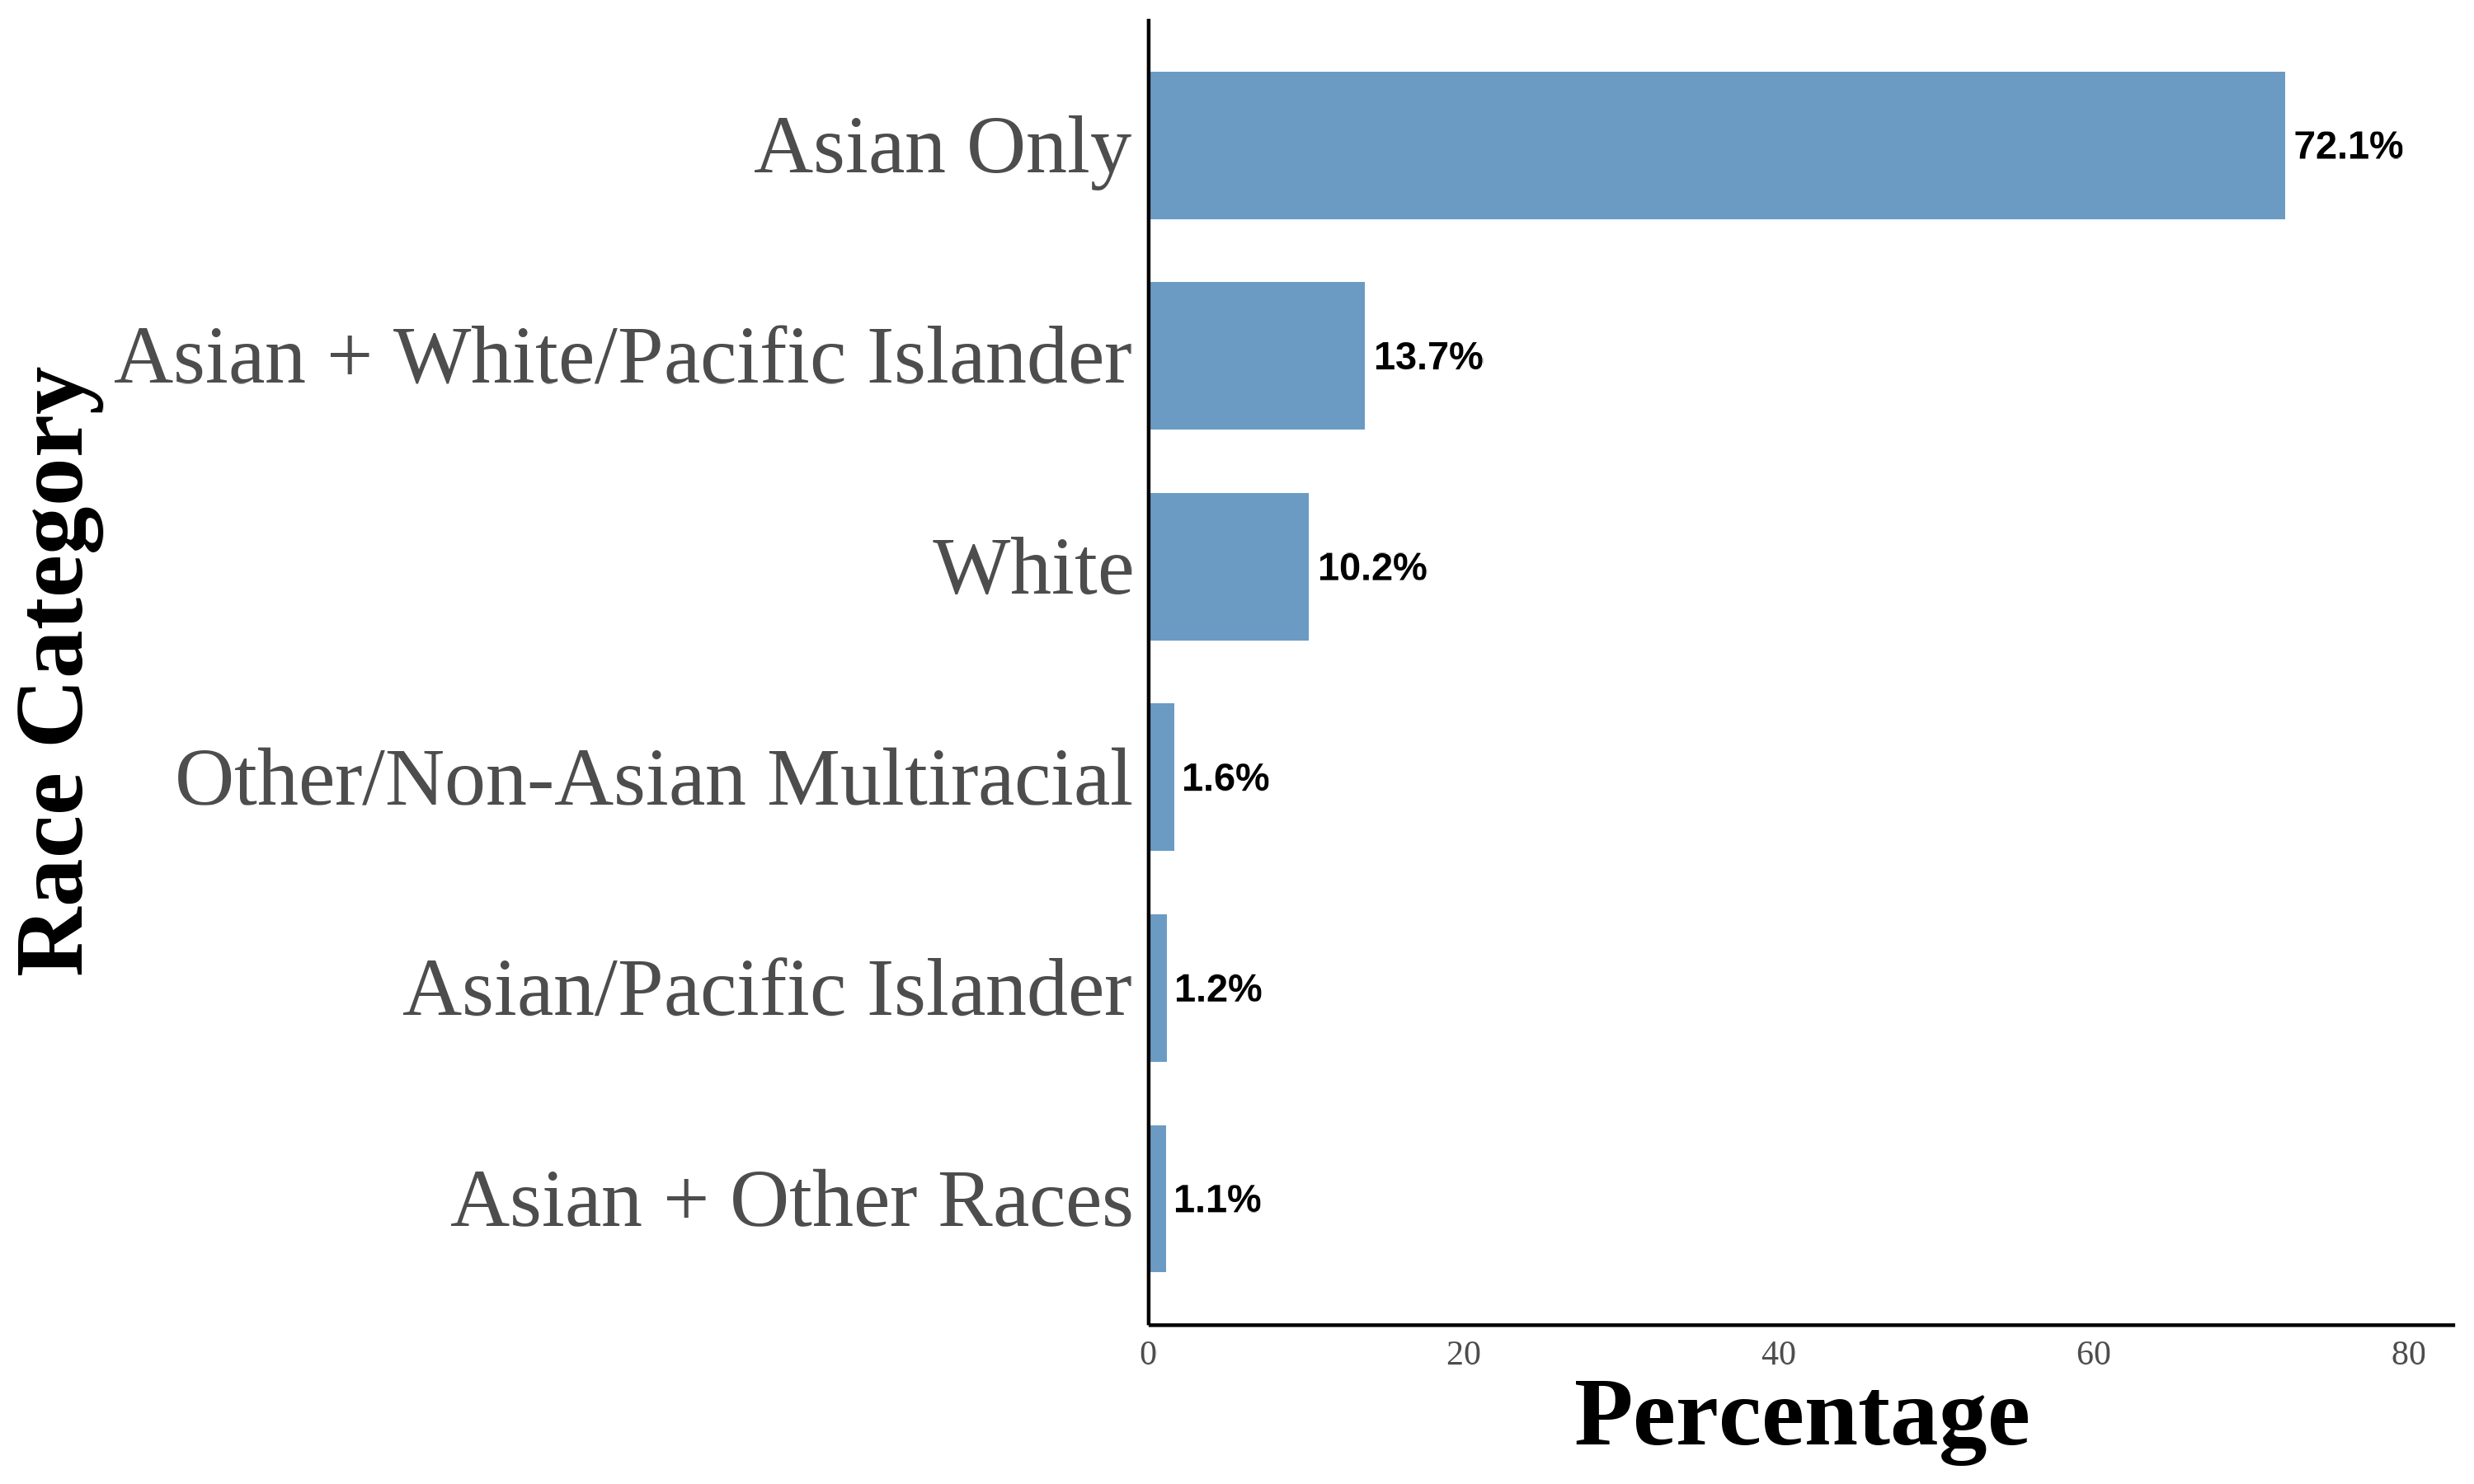
\includegraphics[width=1\linewidth]{histogram_asian_american_race_secondgen.png}
\end{subfigure}
\hfill
\begin{subfigure}{.48\textwidth}
\caption{Second Generation: Asian Fathers-Asian Mothers}
\centering
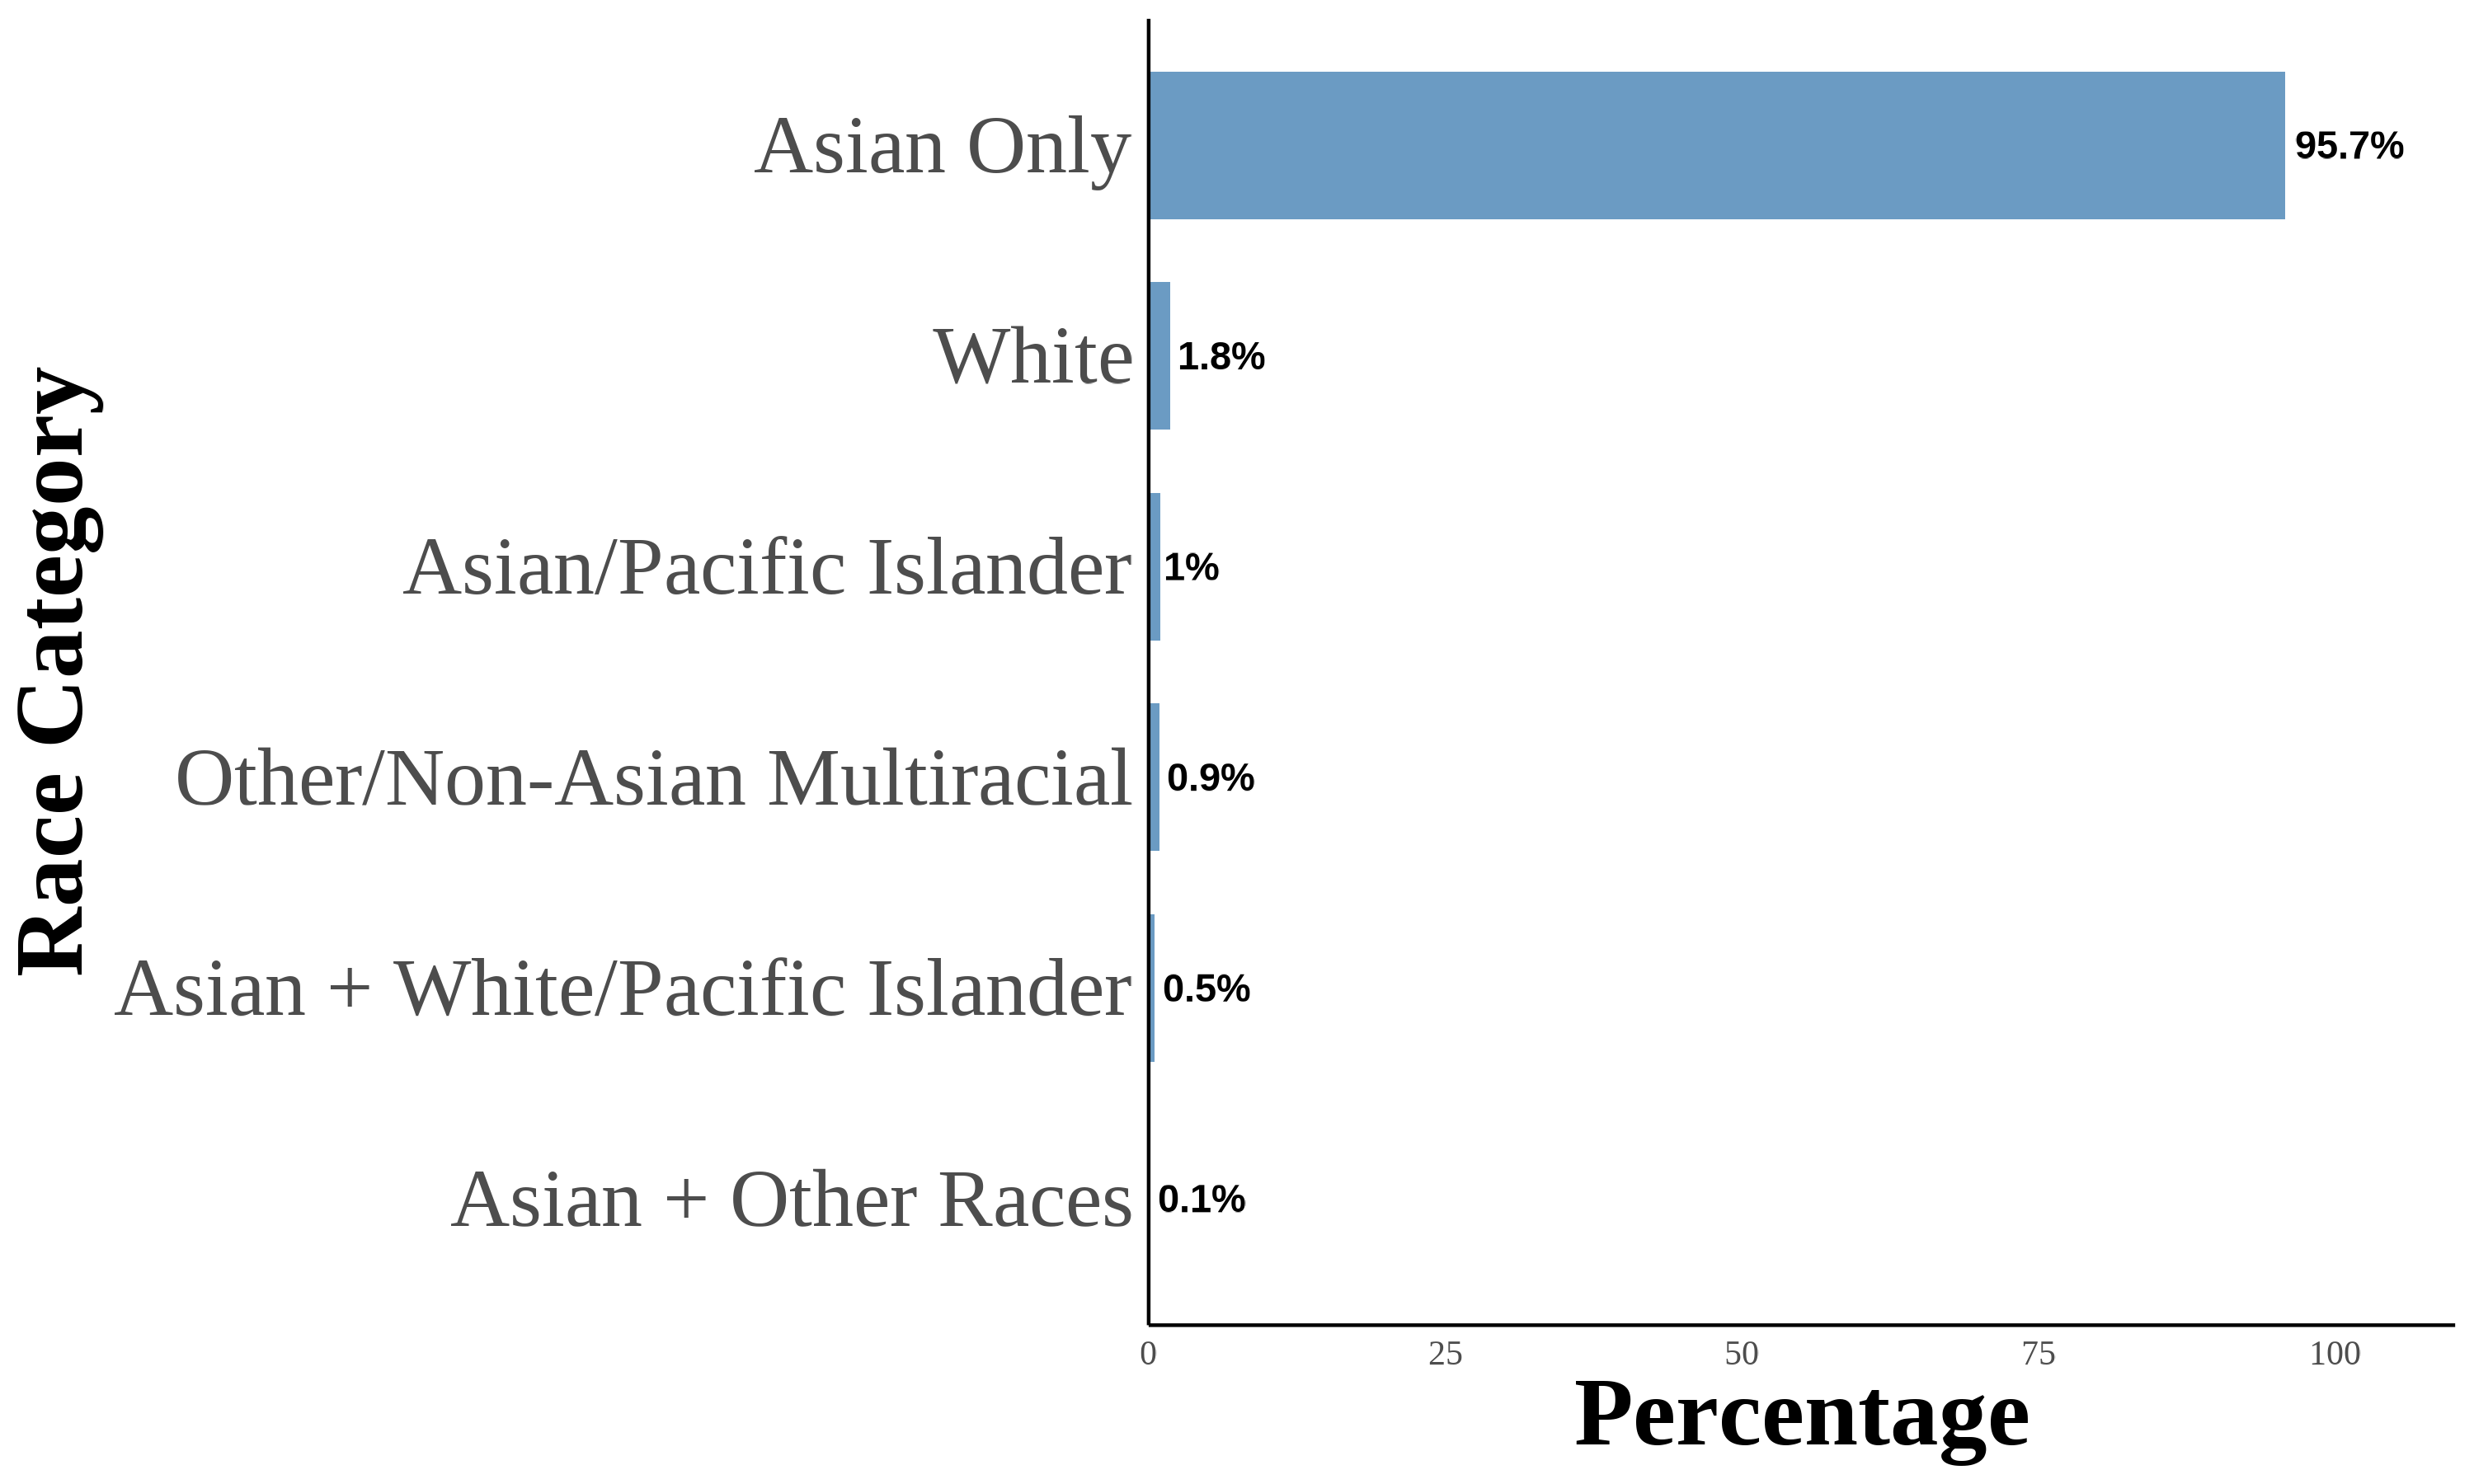
\includegraphics[width=1\linewidth]{histogram_asian_american_race_secondgen_AA.png}
\end{subfigure}

\vspace{1cm}

% Bottom row
\begin{subfigure}{.48\textwidth}
\caption{Second Generation: Asian Fathers-White Mothers}
\centering
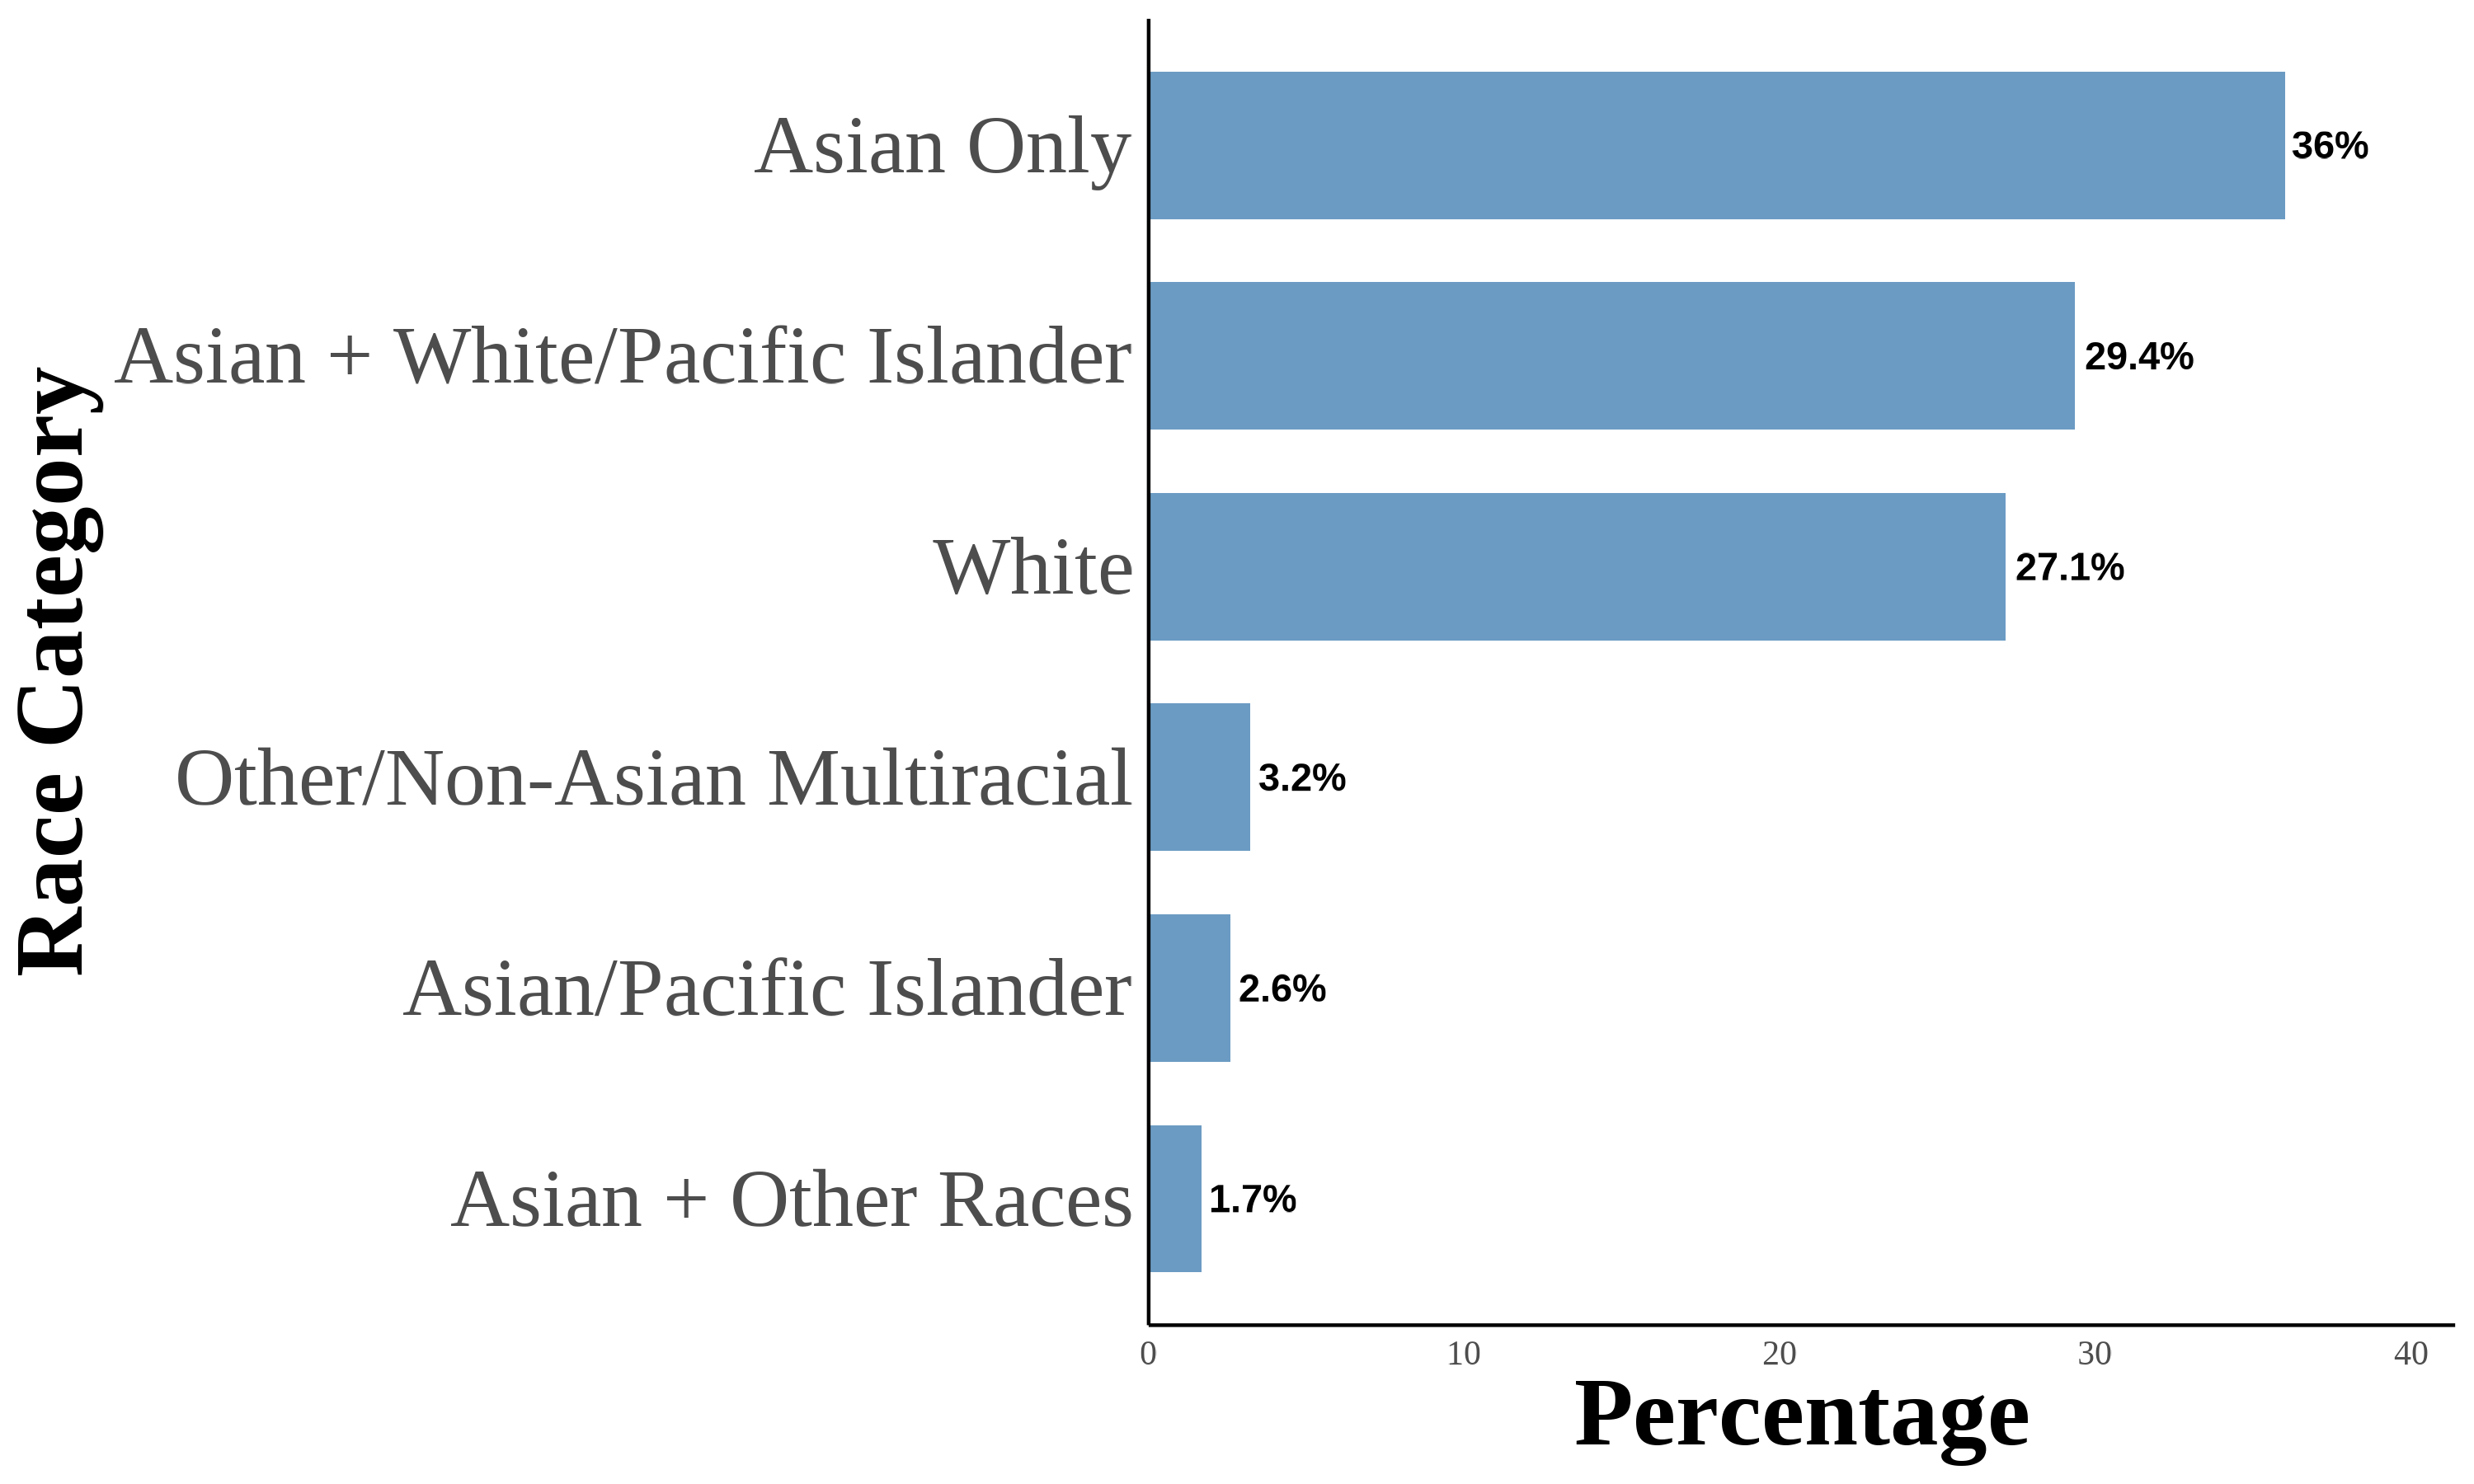
\includegraphics[width=1\linewidth]{histogram_asian_american_race_secondgen_AW.png}
\end{subfigure}
\hfill
\begin{subfigure}{.48\textwidth}
\caption{Second Generation: White Fathers-Asian Mothers}
\centering
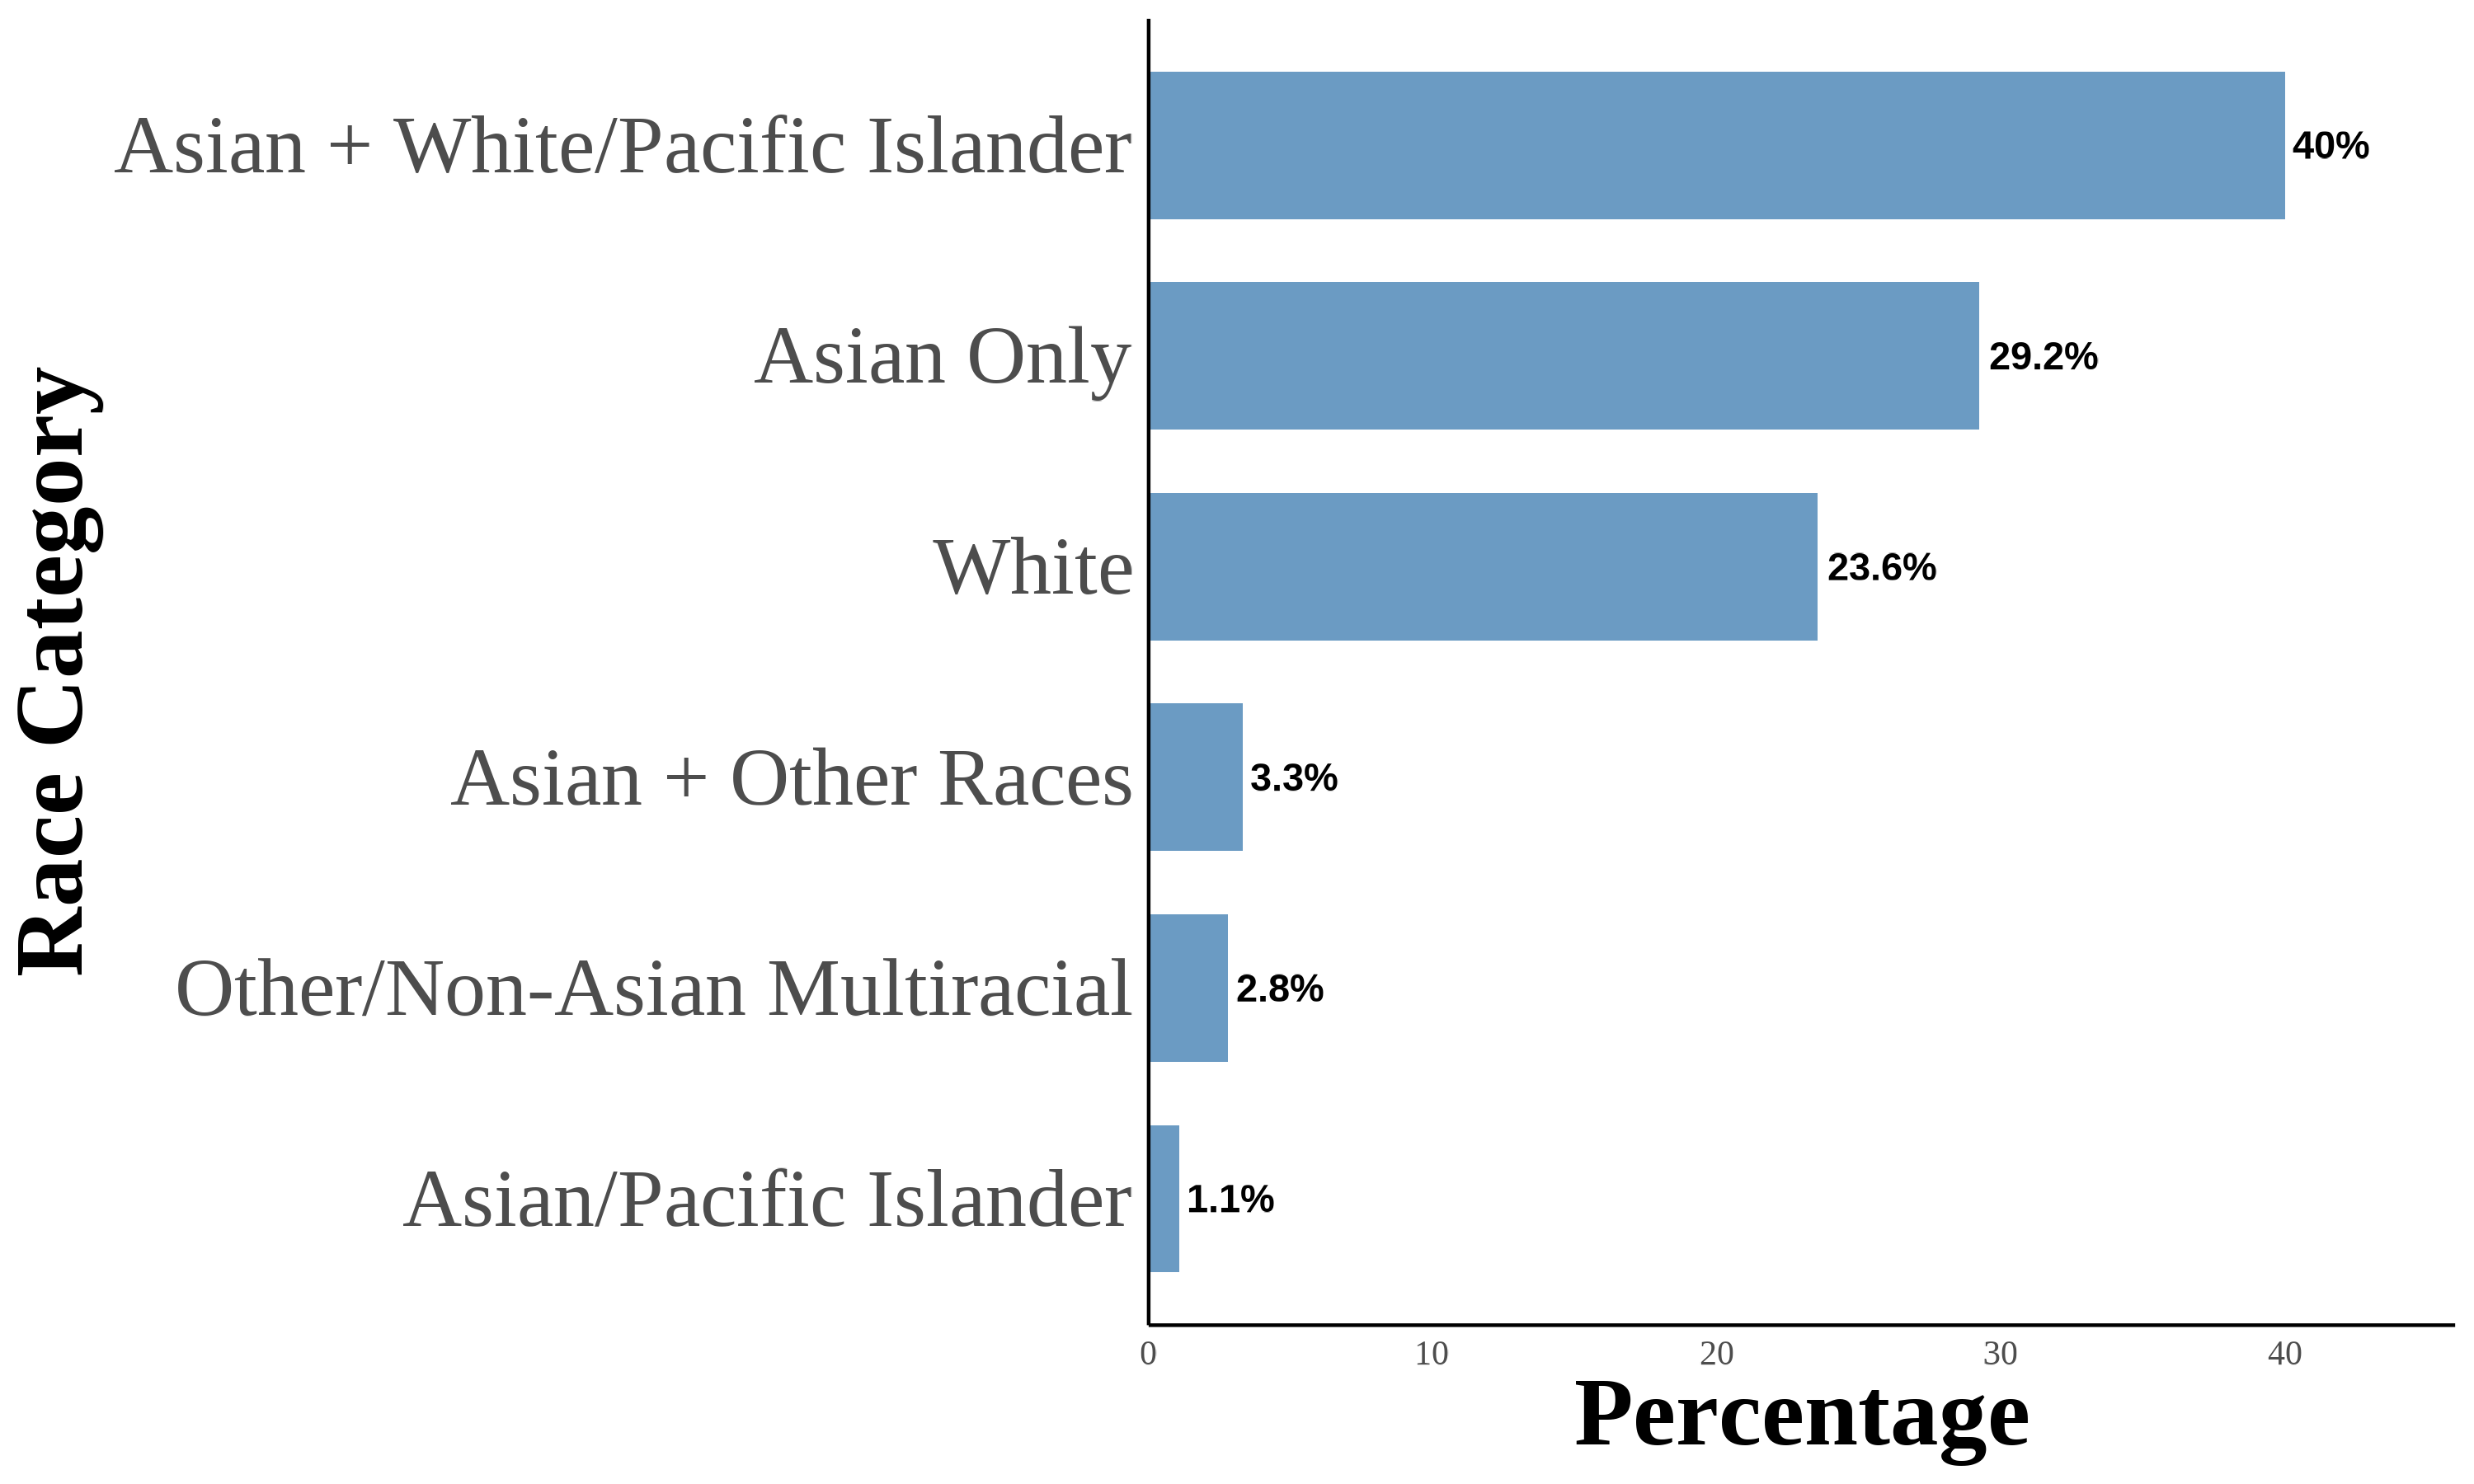
\includegraphics[width=1\linewidth]{histogram_asian_american_race_secondgen_WA.png}
\end{subfigure}

\caption*{\footnotesize{This figure shows the distribution of Asian racial identity among respondents. 
The data is aggregated from the 2004--2021 Current Population Survey (CPS). 
The sample includes second-generation objectively Asian Americans.
Following \textcite{antmanEthnicAttritionObserved2016,antmanEthnicAttritionAssimilation2020}, 
I utilize birthplace information for individuals, parents, and grandparents to create objective Asian ancestry indicators.
A second-generation Asian American is defined as a native-born individual with at least one parent born in an Asian country. 
The first panel is for second-generation Asian Americans. The second panel is for second-generation Asian Americans with both parents born in an Asian country. 
The third panel is for second-generation Asian Americans with an Asian father and a White mother. 
The fourth panel is for second-generation Asian Americans with a White father and an Asian mother.
}}
\end{figure}
\end{landscape}

\pagebreak
\newpage

\pagebreak
\newpage

\begin{landscape}
\begin{figure}[!htb]
\centering
\caption{Asian Racial Identity: Third Generation}
\label{fig:histogram-thirdgen}

% Top row - 3 graphs
\begin{subfigure}{.32\textwidth}
\caption{All Third Generation}
\centering
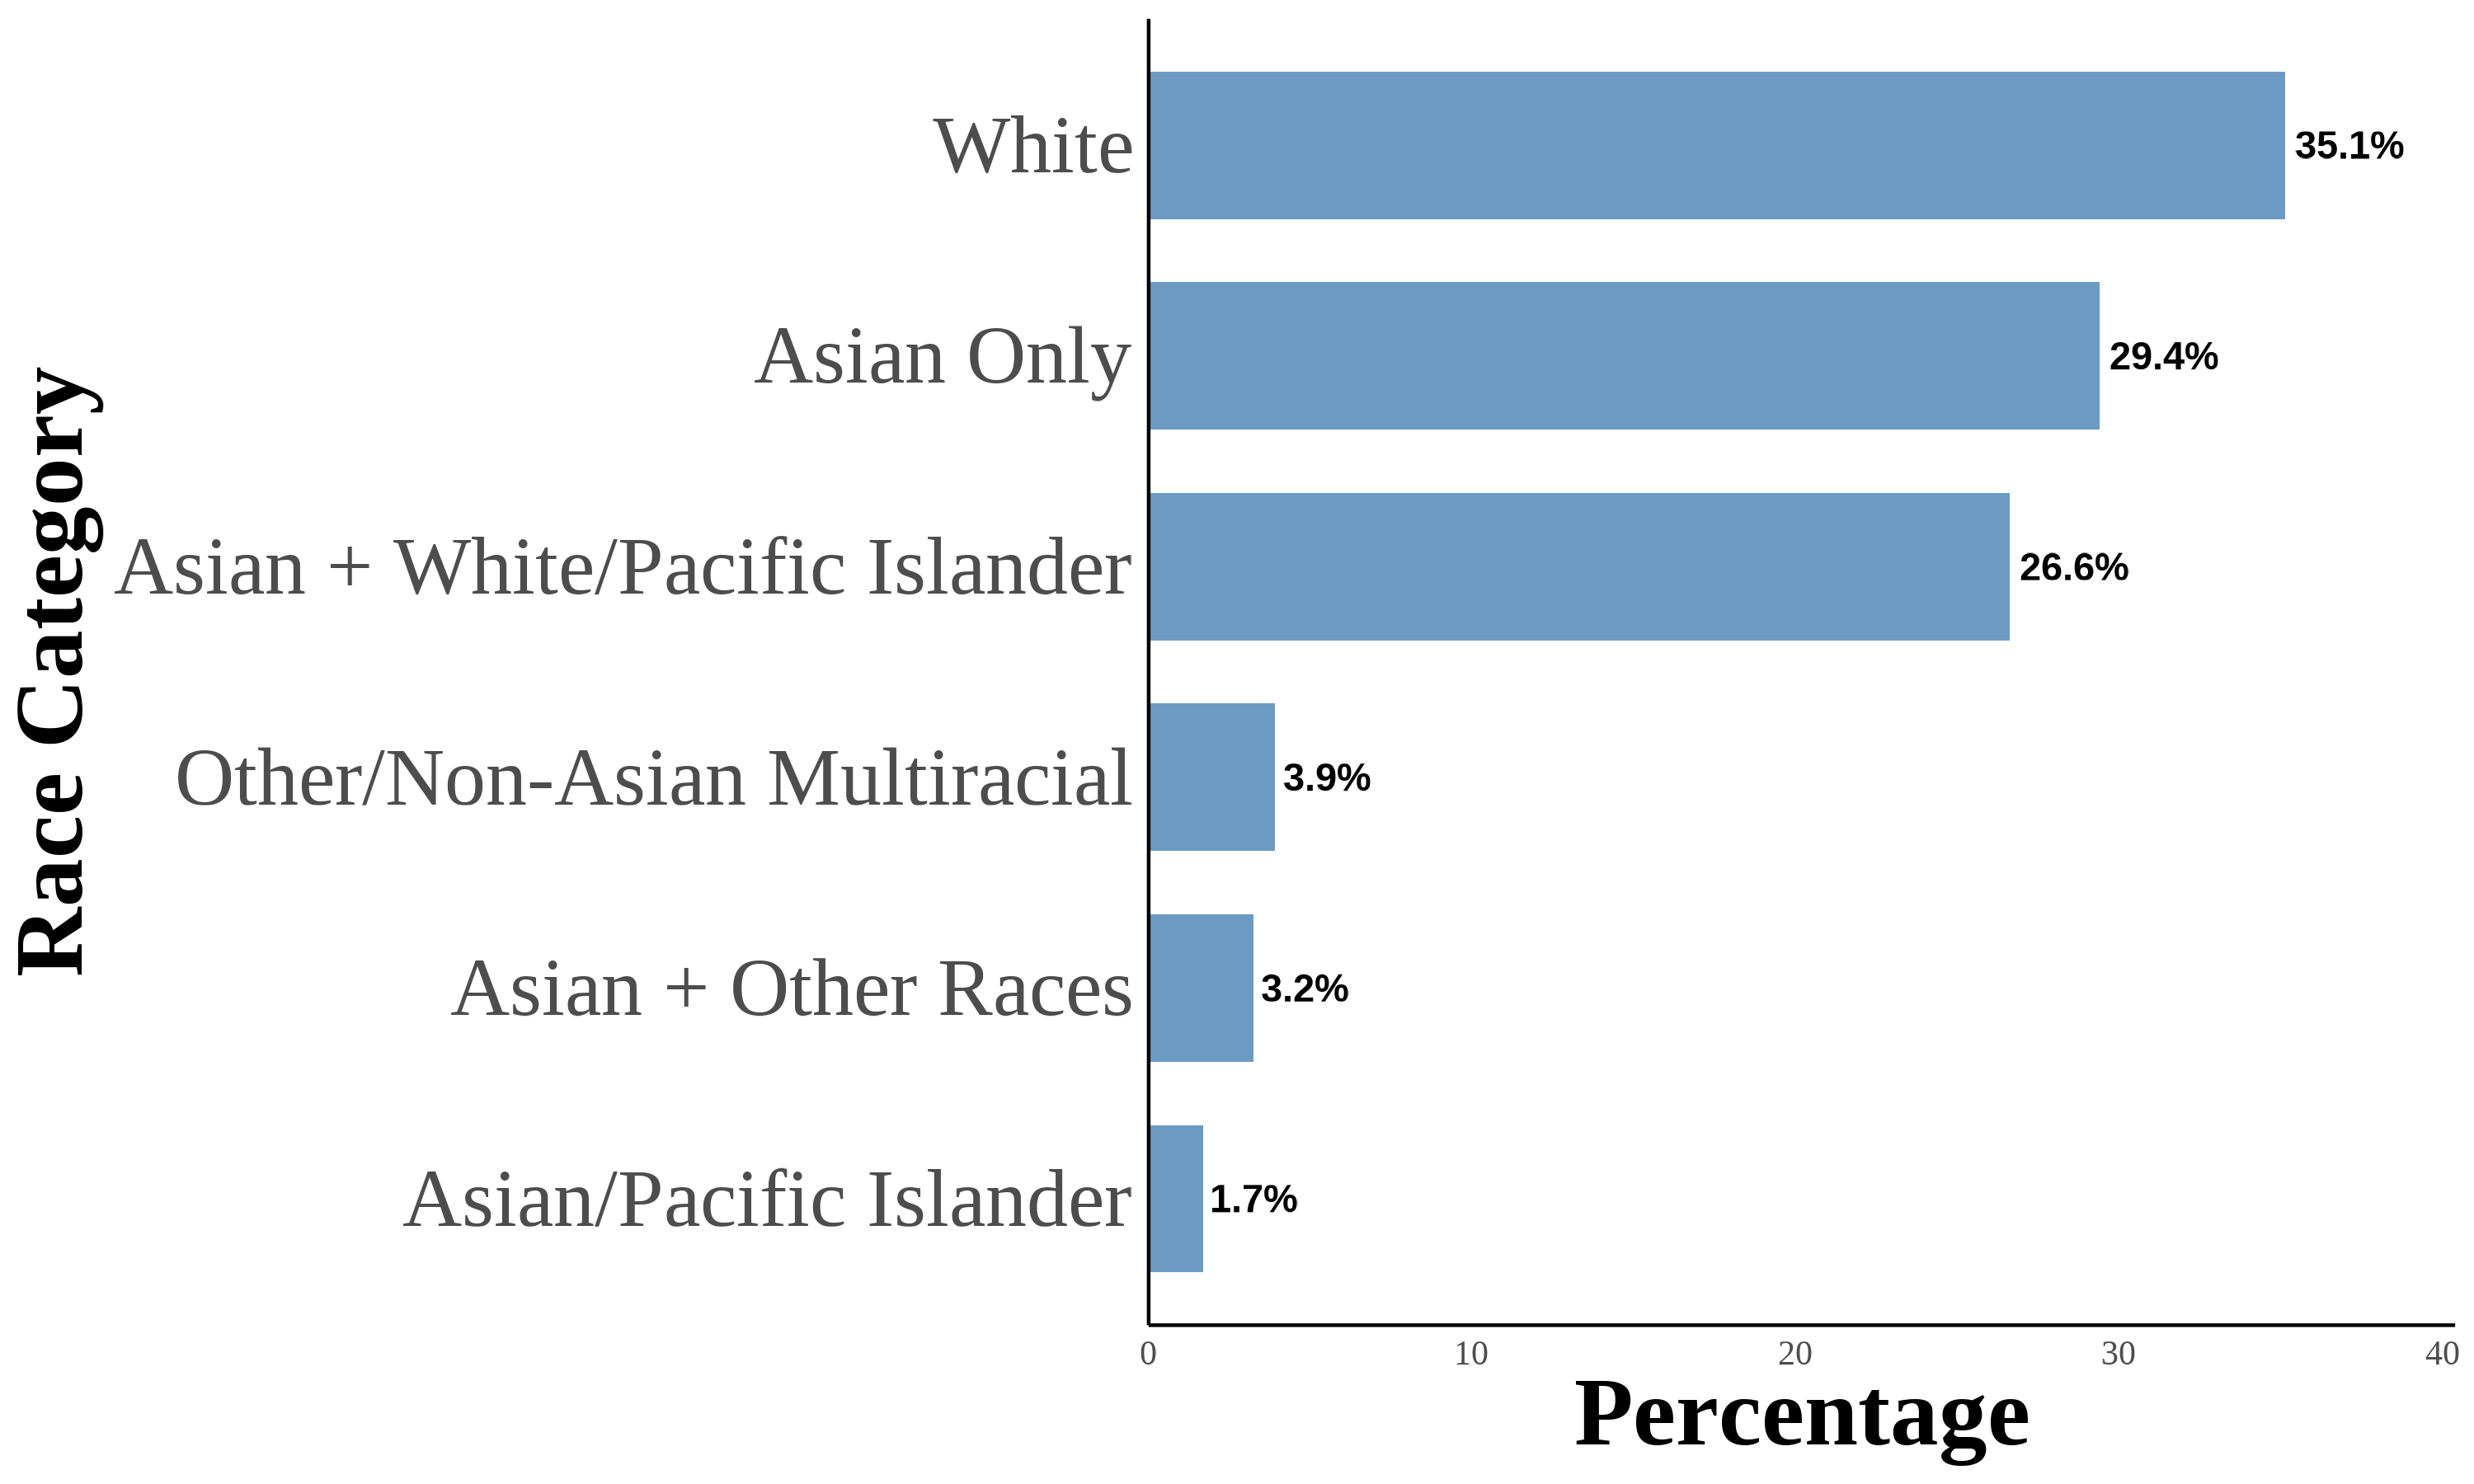
\includegraphics[width=1\linewidth]{histogram_asian_american_race_thirdgen.png}
\end{subfigure}
\hfill
\begin{subfigure}{.32\textwidth}
\caption{Third Generation: One Asian Grandparent}
\centering
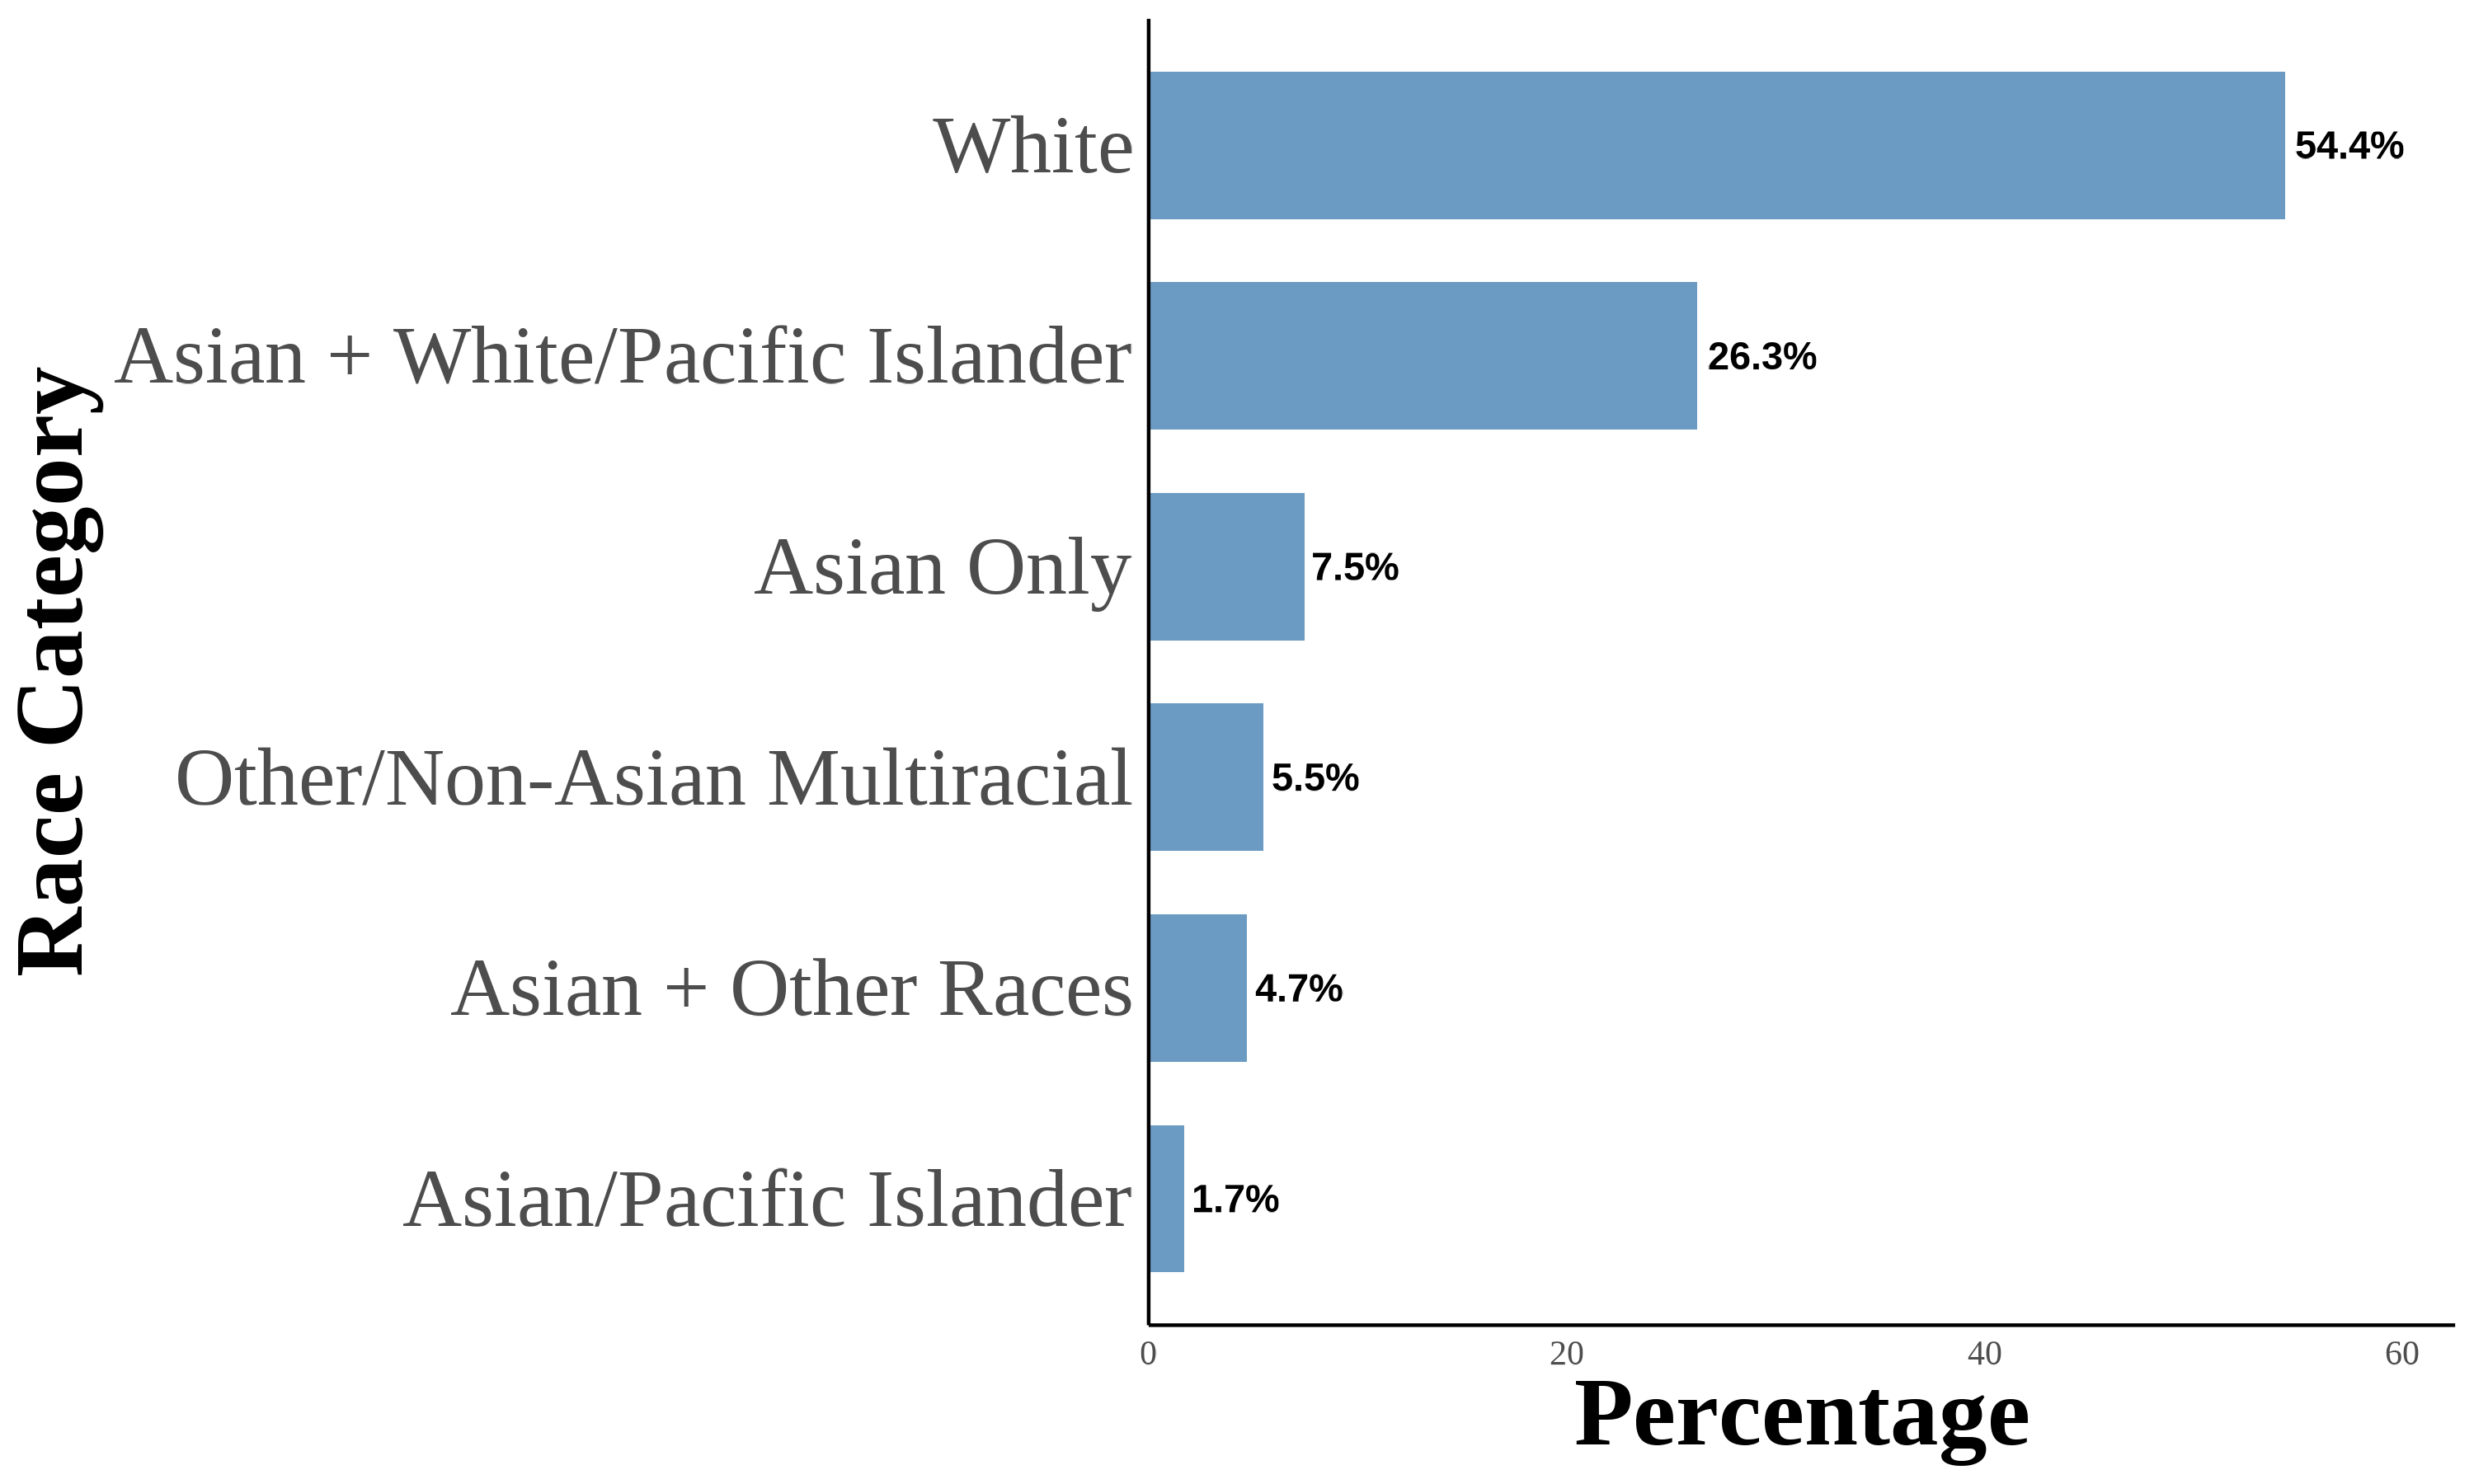
\includegraphics[width=1\linewidth]{histogram_asian_american_race_thirdgen_oneasiangran.png}
\end{subfigure}
\hfill
\begin{subfigure}{.32\textwidth}
\caption{Third Generation: Two Asian Grandparents}
\centering
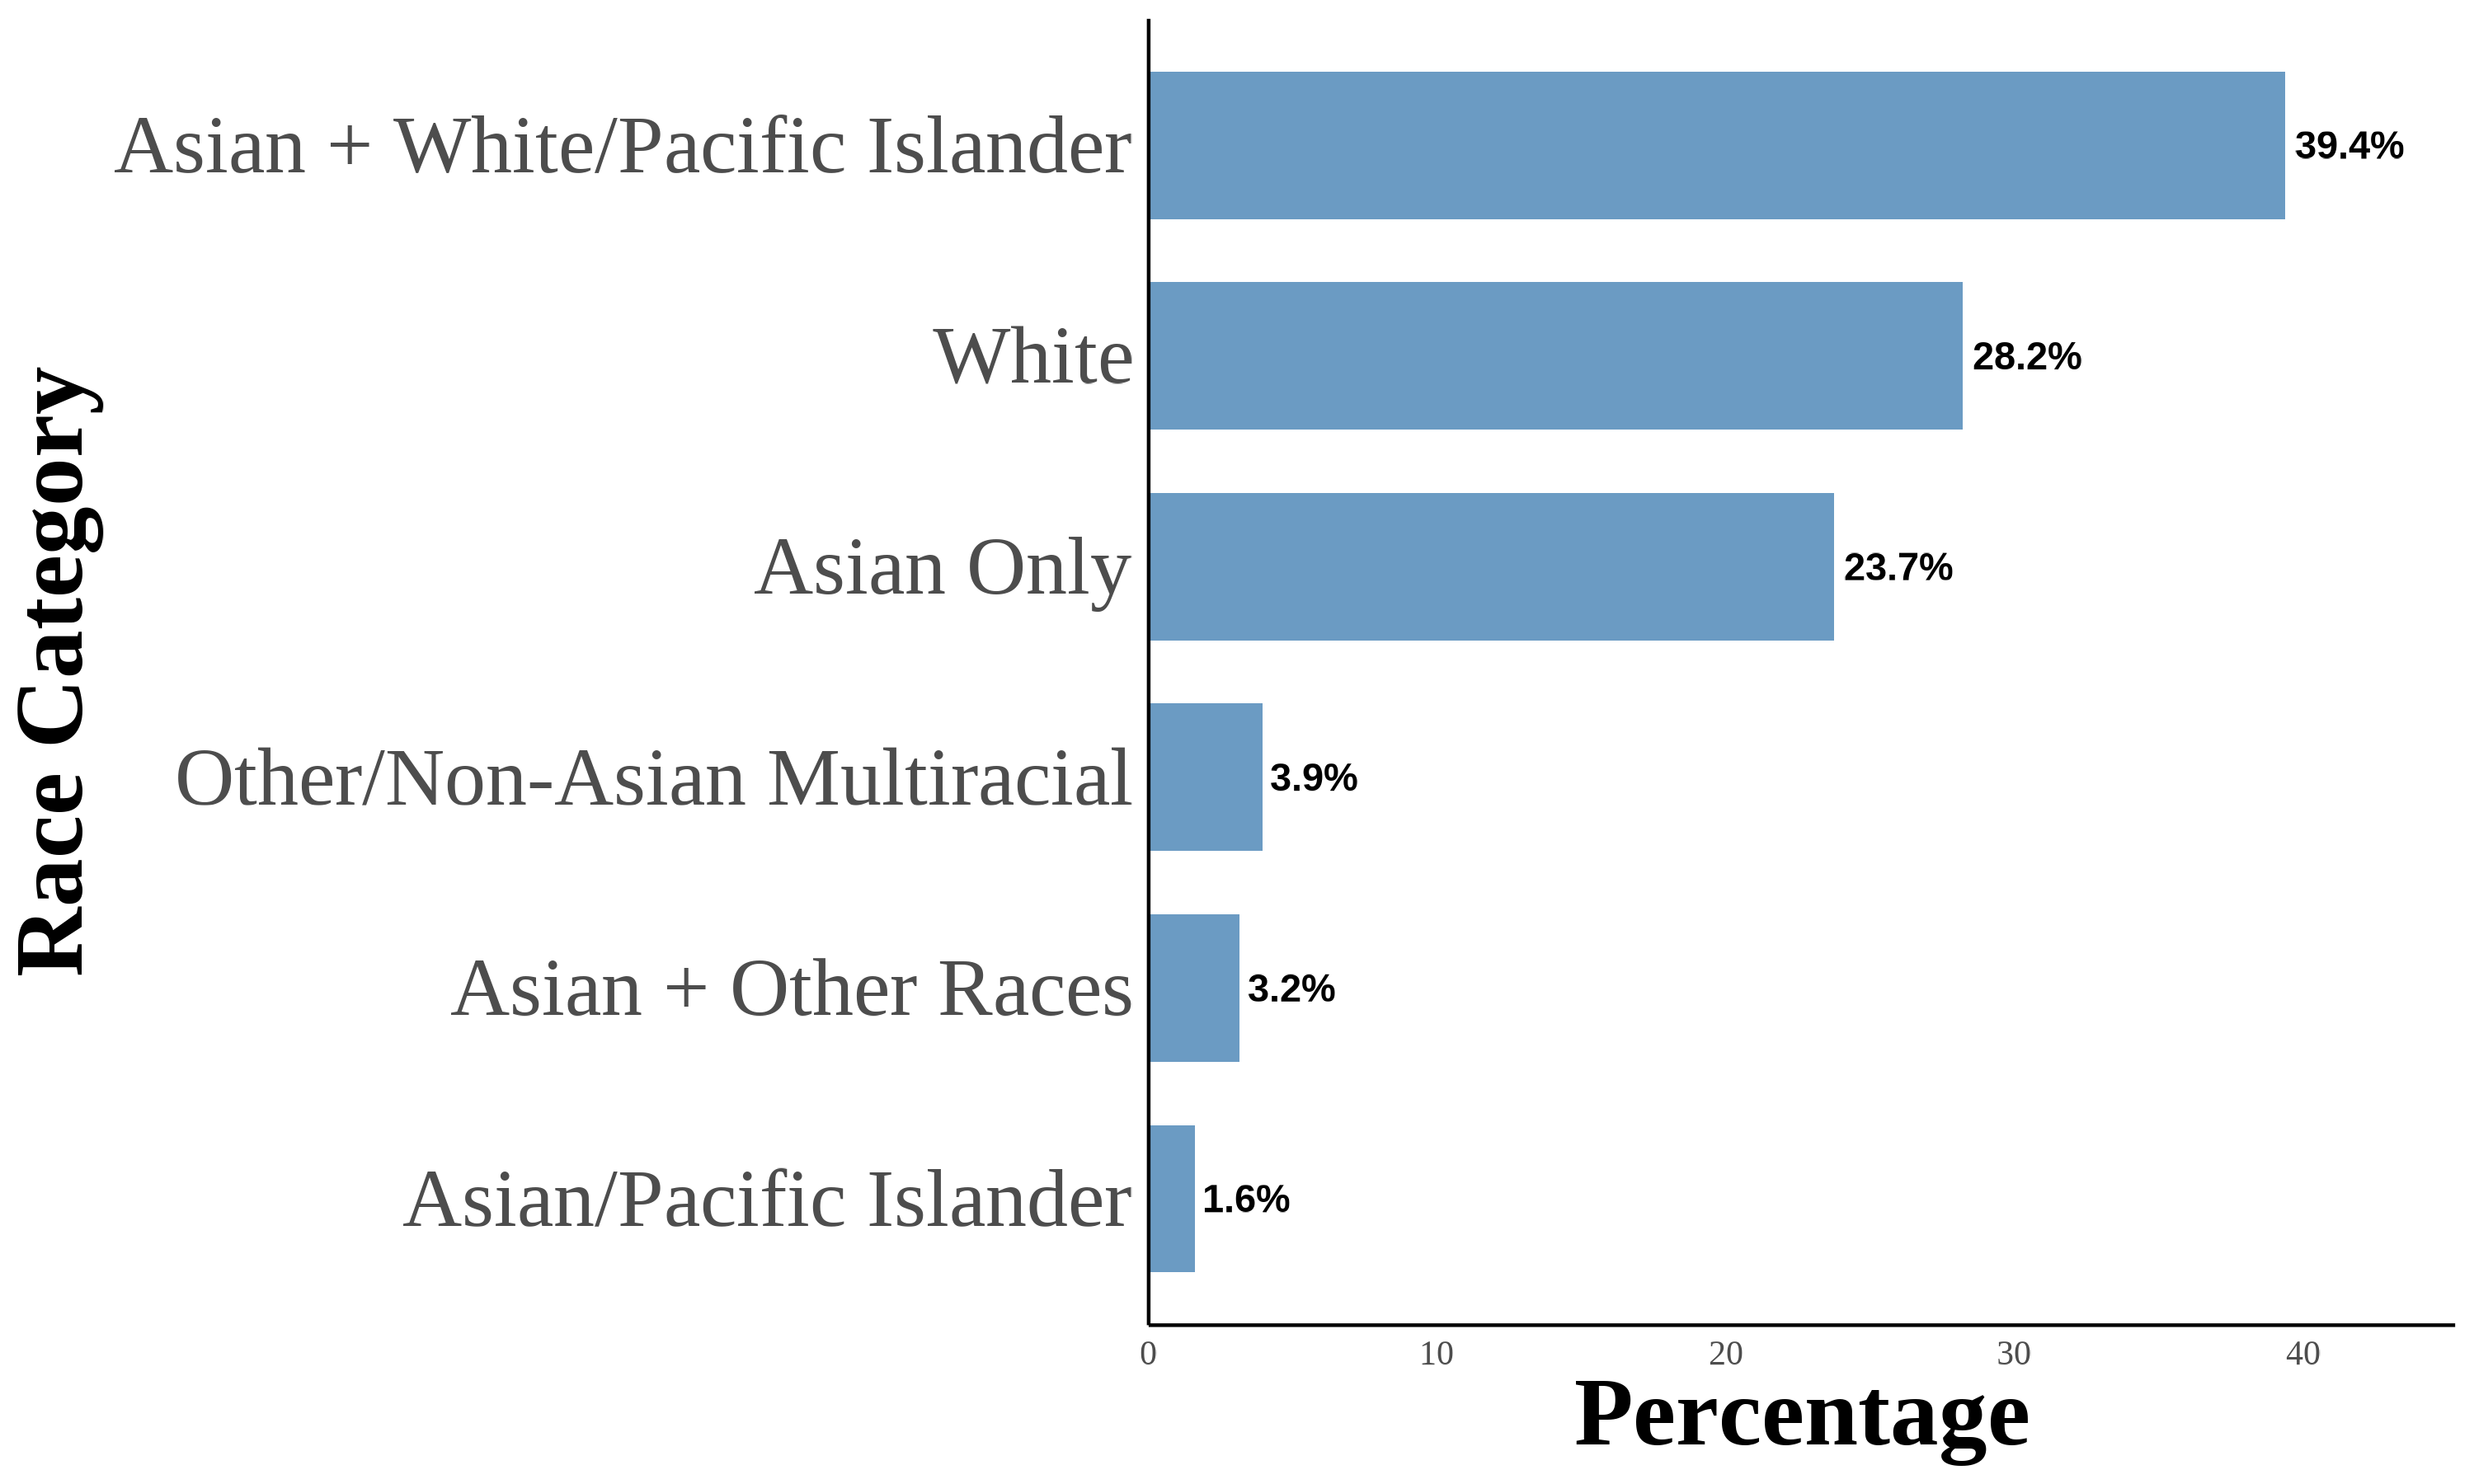
\includegraphics[width=1\linewidth]{histogram_asian_american_race_thirdgen_twoasiangran.png}
\end{subfigure}

\vspace{1cm}

% Bottom row - 2 graphs centered with more space
\hspace*{\fill}
\begin{subfigure}{.4\textwidth}
\caption{Third Generation: Three Asian Grandparents}
\centering
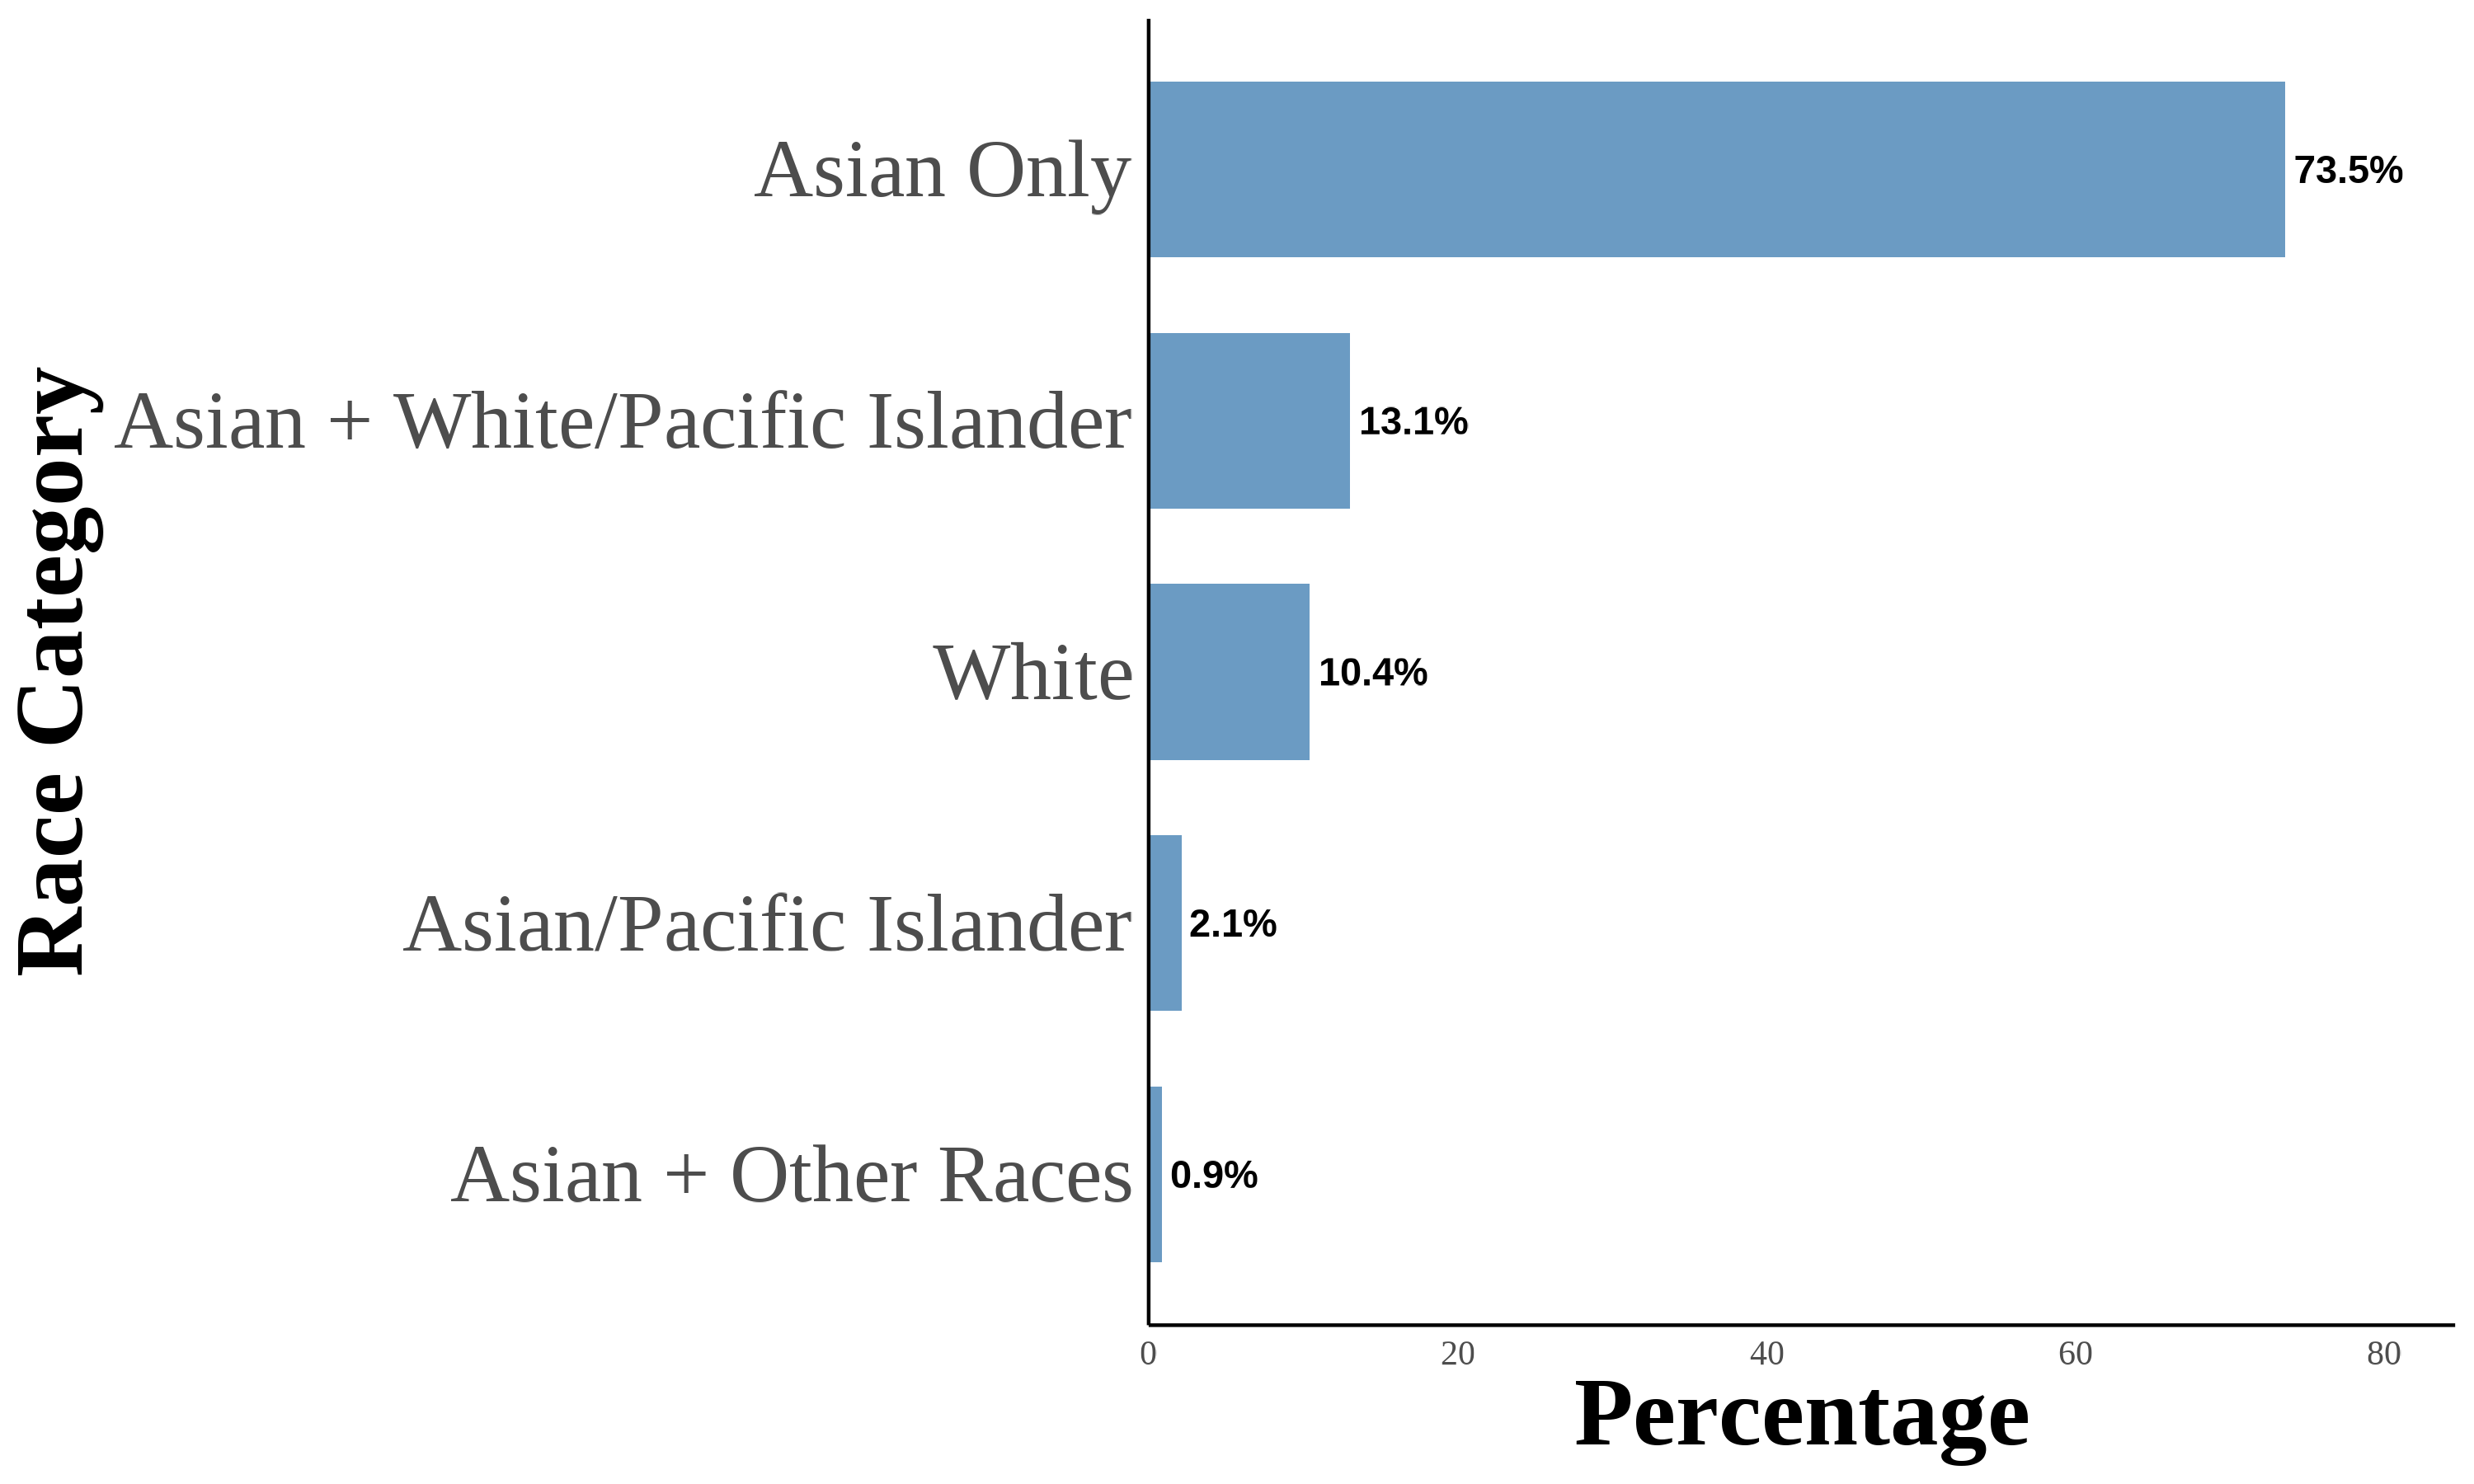
\includegraphics[width=1\linewidth]{histogram_asian_american_race_thirdgen_threeasiangran.png}
\end{subfigure}
\hfill
\begin{subfigure}{.4\textwidth}
\caption{Third Generation: Four Asian Grandparents}
\centering
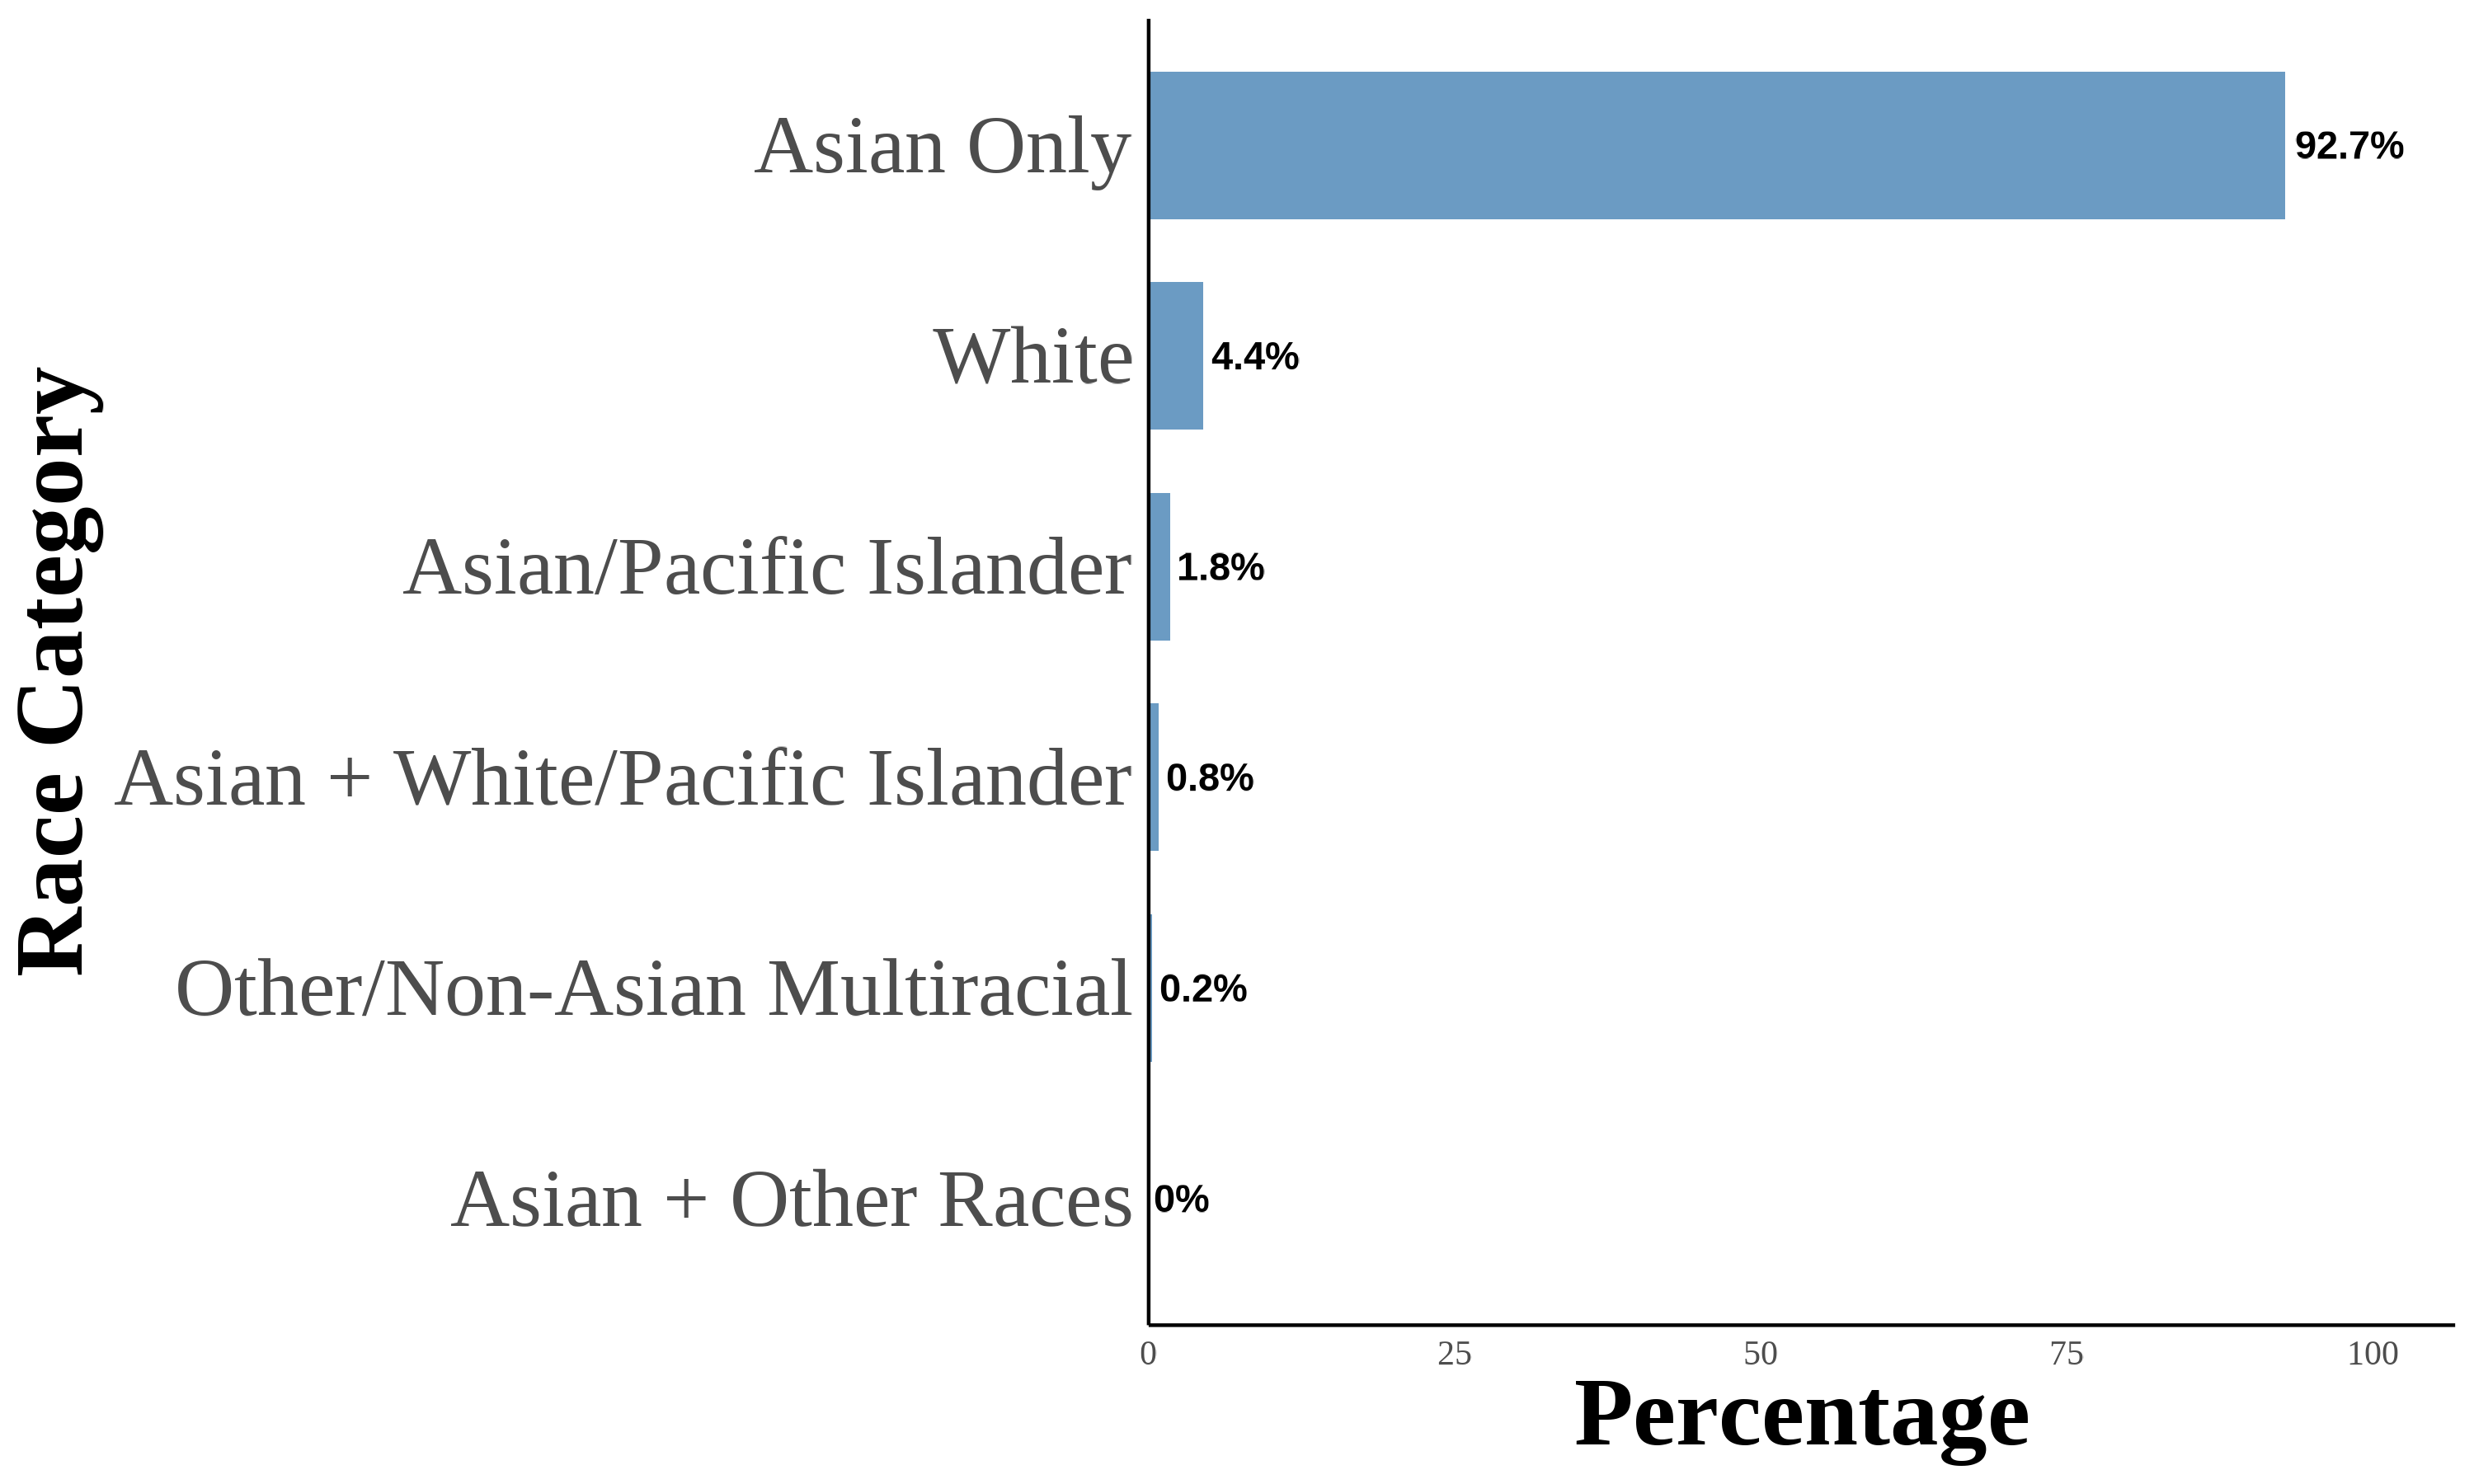
\includegraphics[width=1\linewidth]{histogram_asian_american_race_thirdgen_fourasiangran.png}
\end{subfigure}
\hspace*{\fill}

\caption*{\footnotesize{This figure shows the distribution of Asian racial identity among respondents. 
The data is aggregated from the 2004--2021 Current Population Survey (CPS). 
The sample includes second-generation objectively Asian Americans.
Following \textcite{antmanEthnicAttritionObserved2016,antmanEthnicAttritionAssimilation2020}, 
I utilize birthplace information for individuals, parents, and grandparents to create objective Asian ancestry indicators.
A third-generation Asian American is defined as a native-born individual with native-born parents and at least one grandparent born in an Asian country. 
The first panel is for third-generation Asian Americans. The second panel is for third-generation Asian Americans with one grandparent born in an Asian country. 
The third panel is for third-generation Asian Americans with two grandparents born in an Asian country. 
The fourth panel is for third-generation Asian Americans with three grandparents born in an Asian country.
The fifth panel is for third-generation Asian Americans with four grandparents born in an Asian country.
}}
\end{figure}
\end{landscape}

\pagebreak
\newpage

\begin{center}
\begin{figure}[!htb]
\centering
\caption{Relationship Between Self-Reported Asian Identity and Bias: By Generation}
\label{plot01-regression-gen}
%First graph
\begin{subfigure}{.48\textwidth}
\caption{All Generations}
\centering
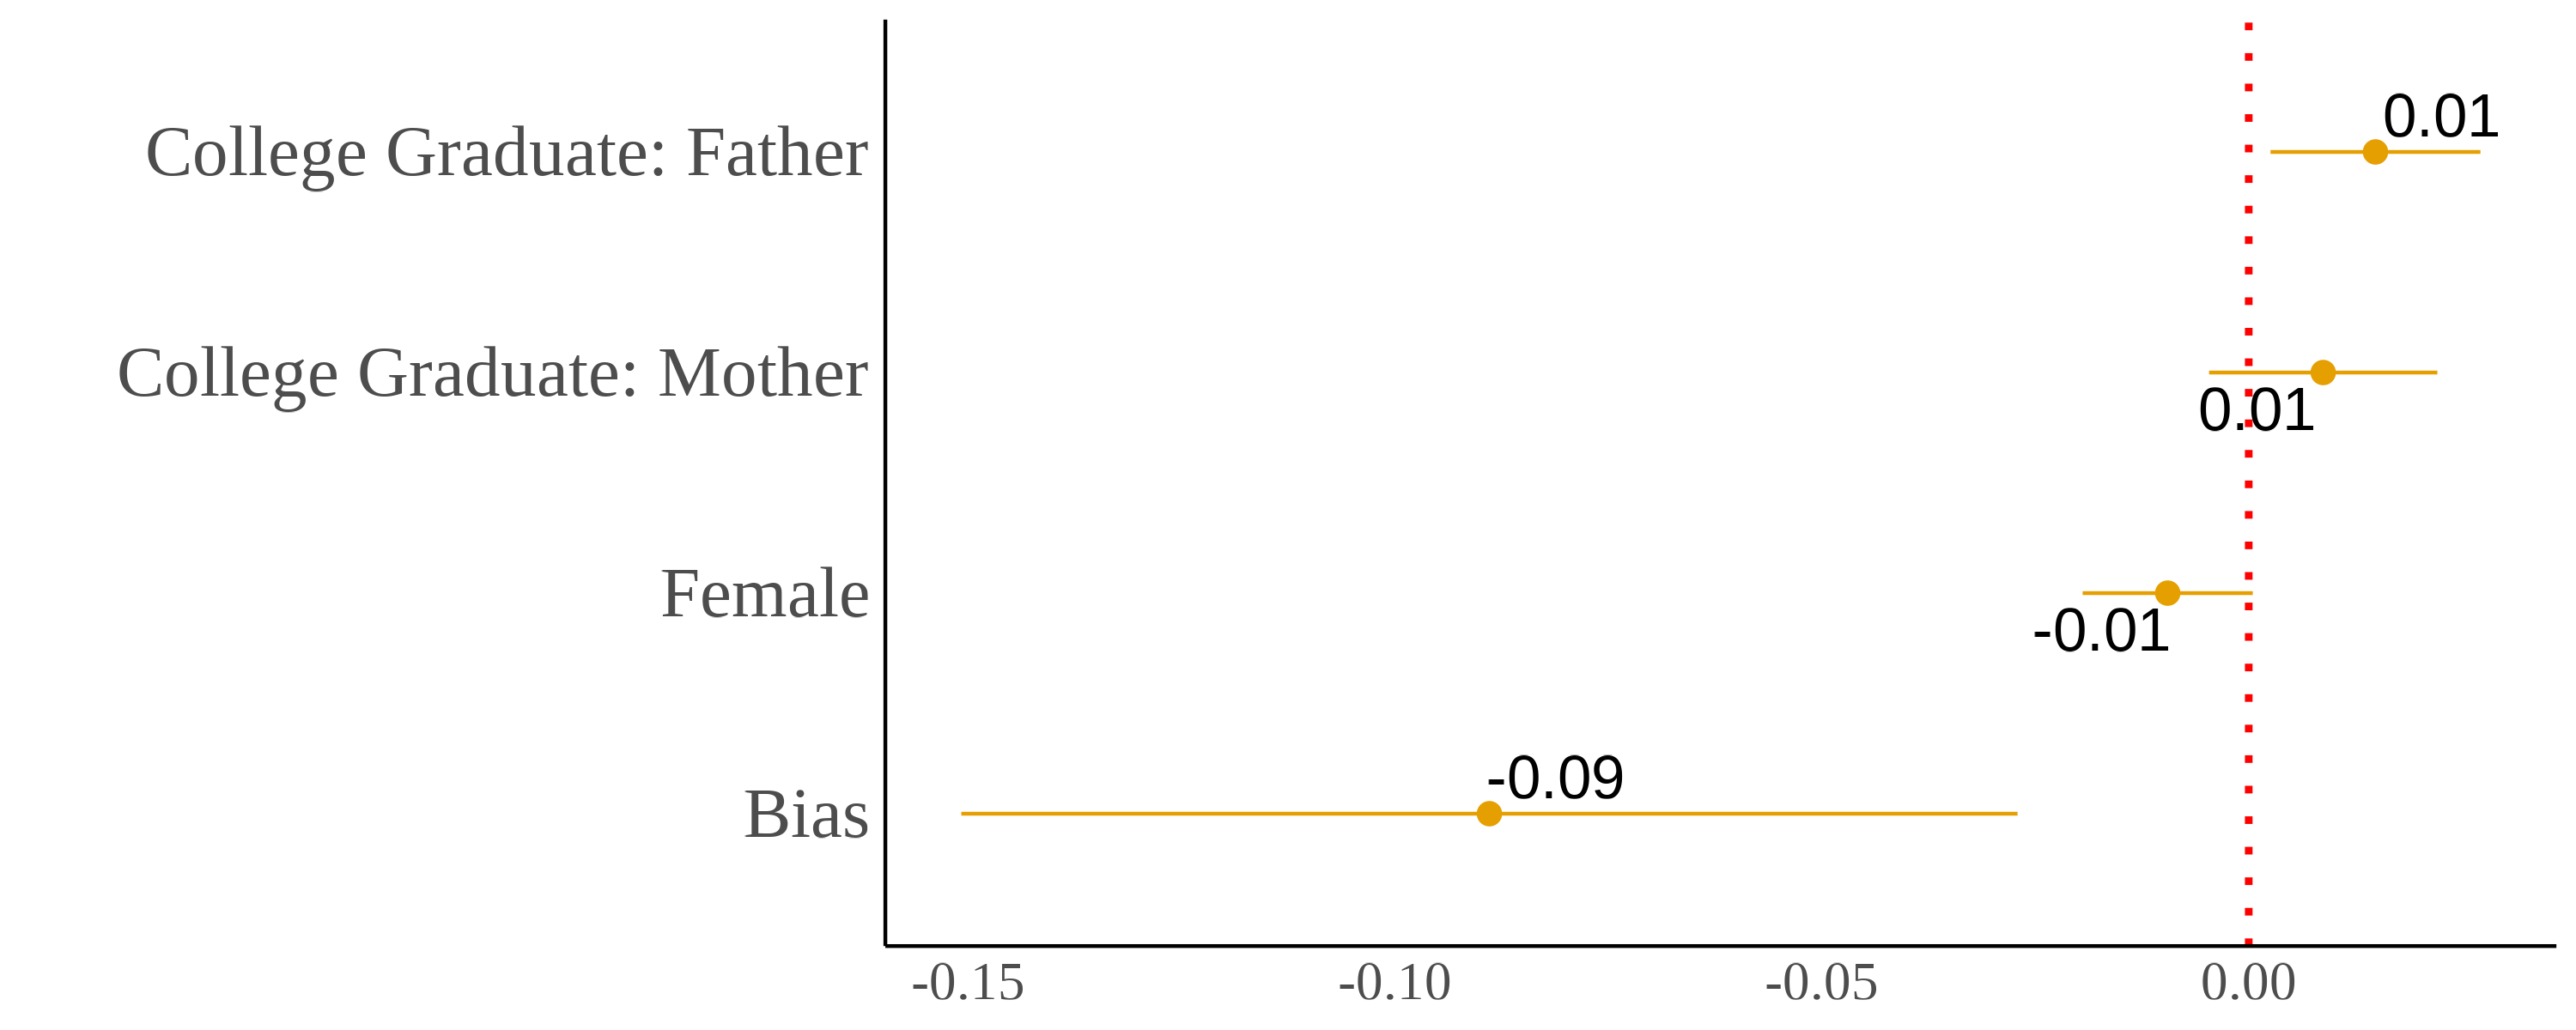
\includegraphics[width=.9\linewidth]{skin-iat-regression-all-gens.png}
\end{subfigure}
\centering
%Second graph
\begin{subfigure}{.48\textwidth}
\caption{First-Generation}
\centering
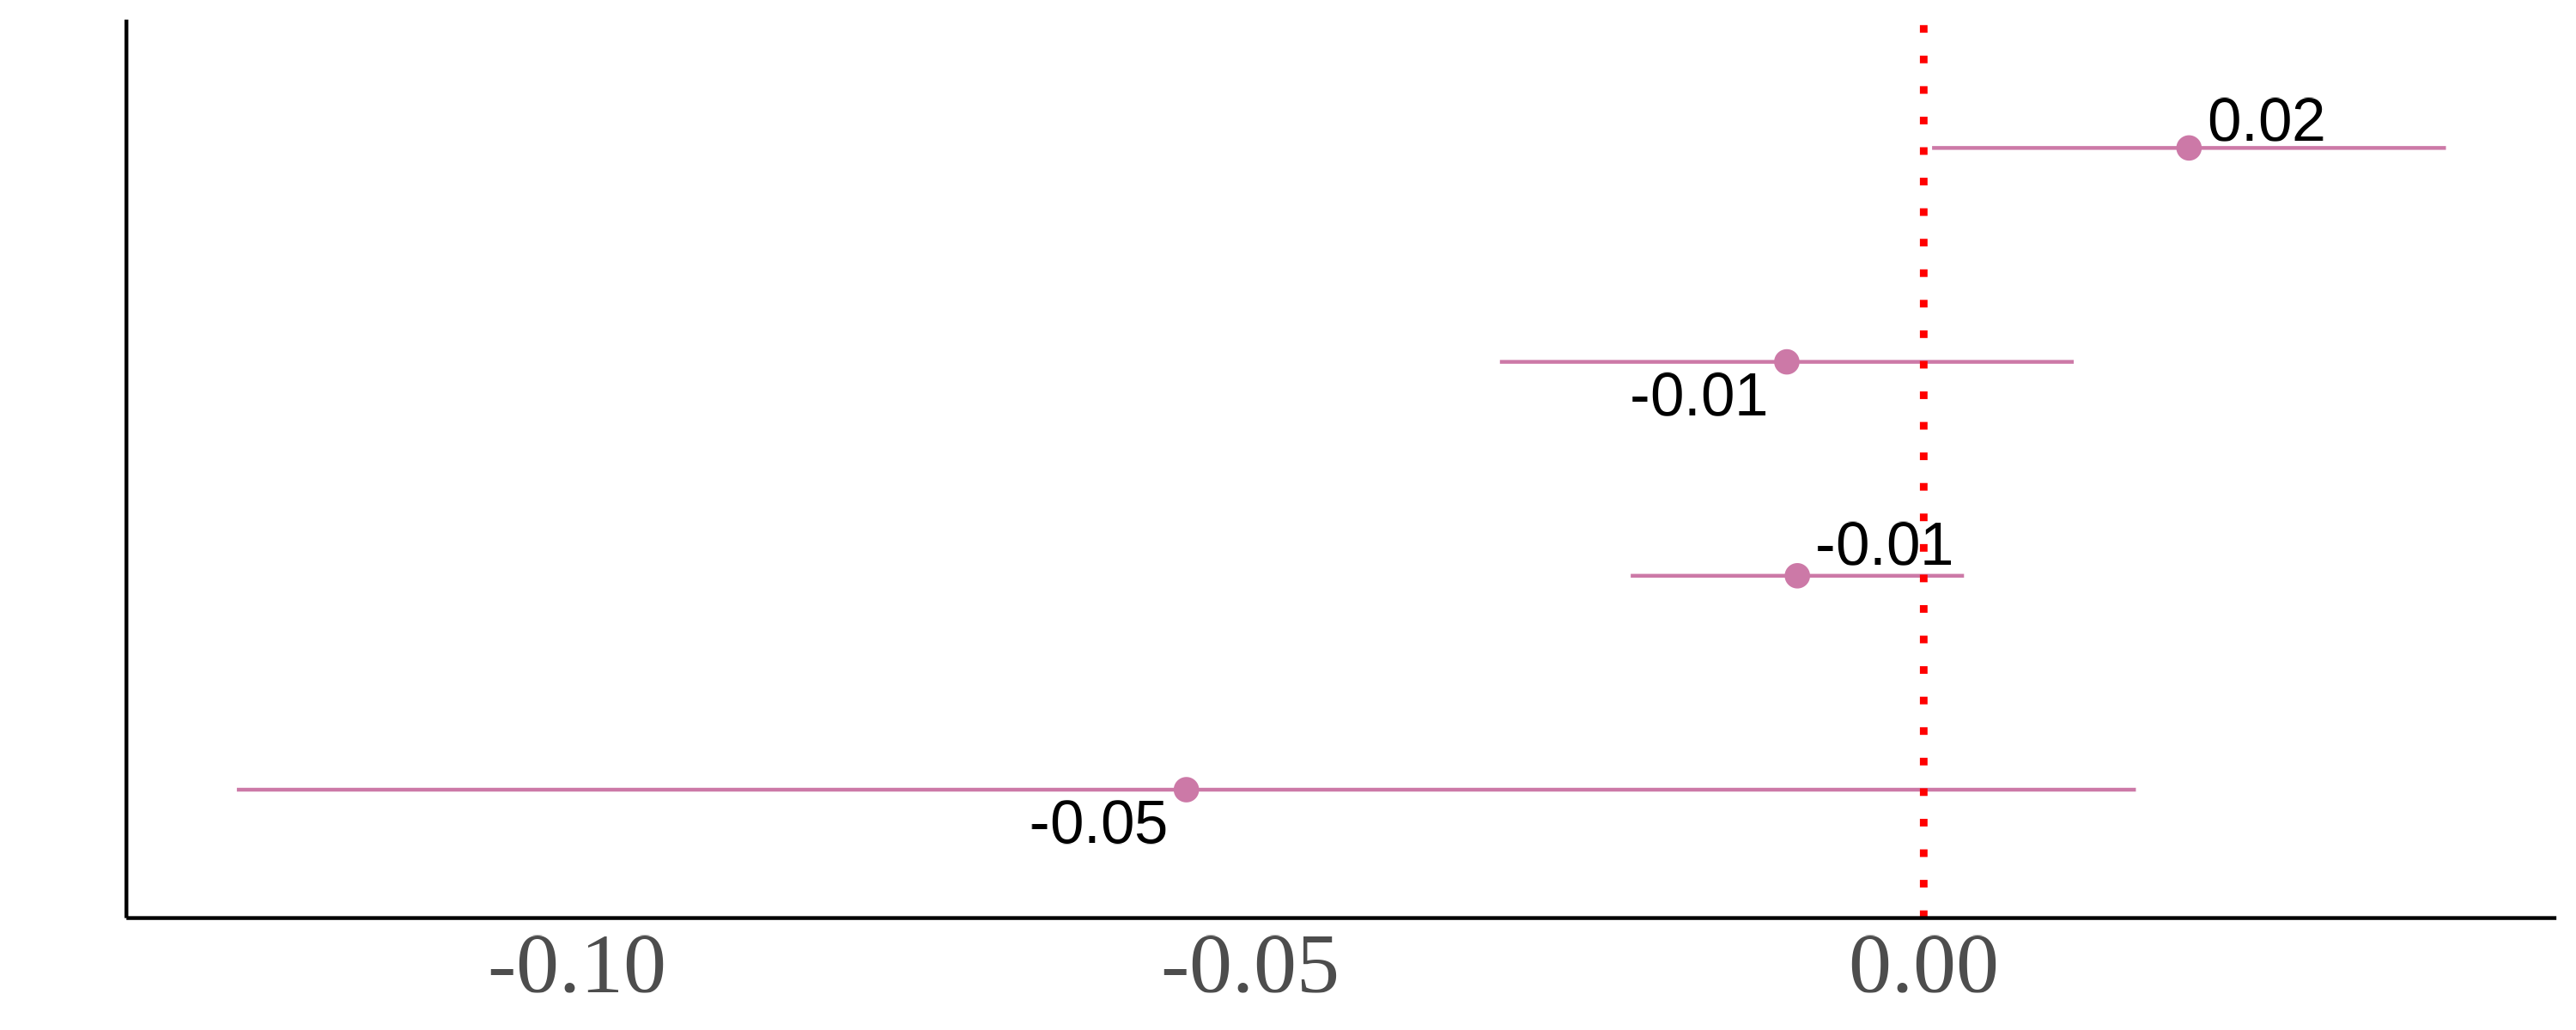
\includegraphics[width=.9\linewidth]{skin-iat-regression-first-gen.png}
\end{subfigure}
%Third Graph
\begin{subfigure}{.48\textwidth}
\caption{Second-Generation}
\centering
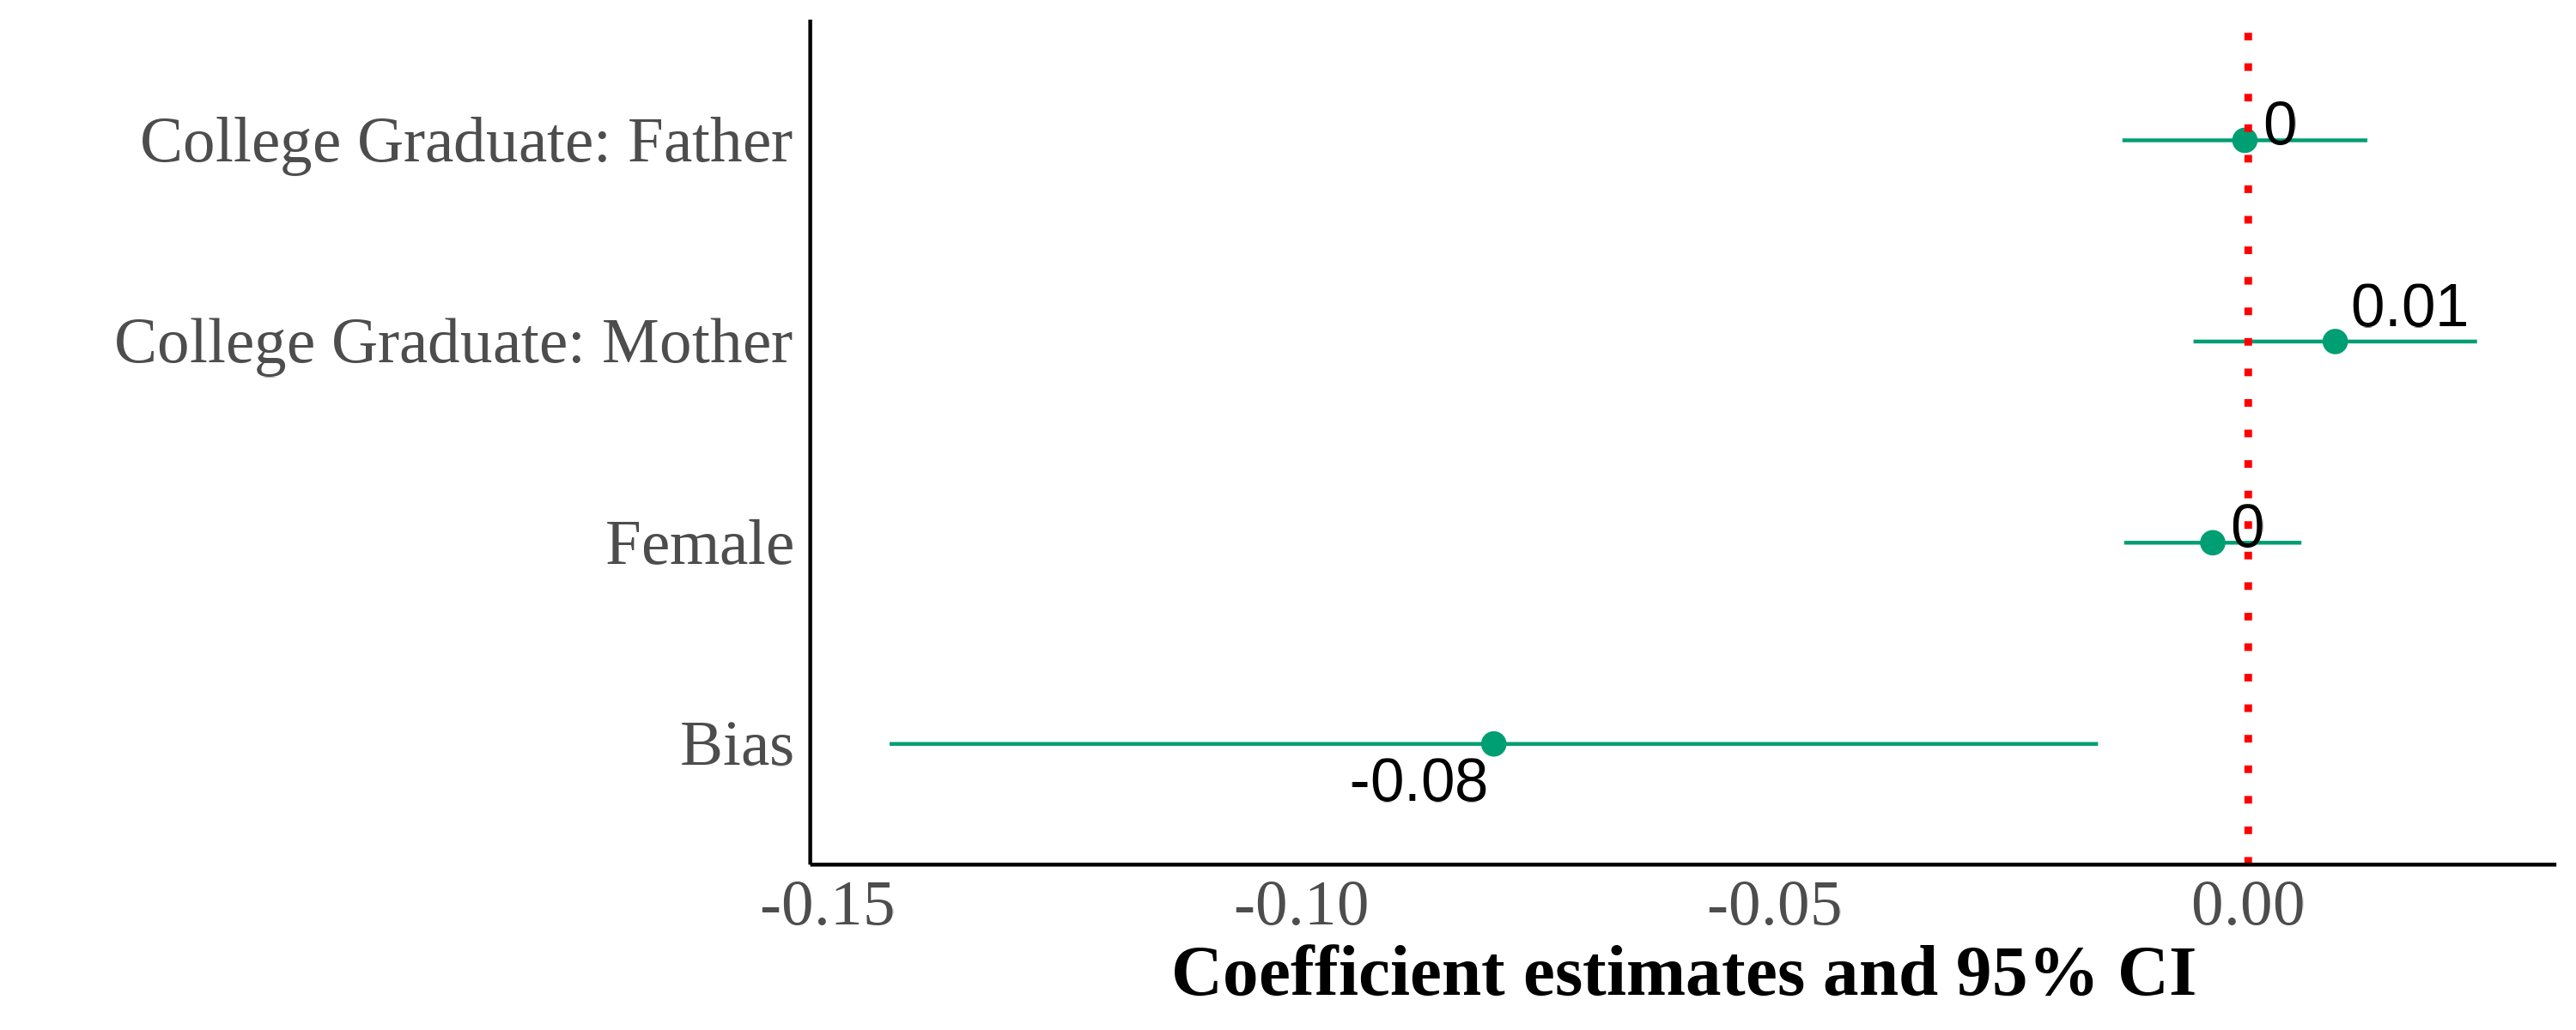
\includegraphics[width=.9\linewidth]{skin-iat-regression-second-gen.png}
\end{subfigure}
%Fourth Graph
\begin{subfigure}{.48\textwidth}
\caption{Third-Generation}
\centering
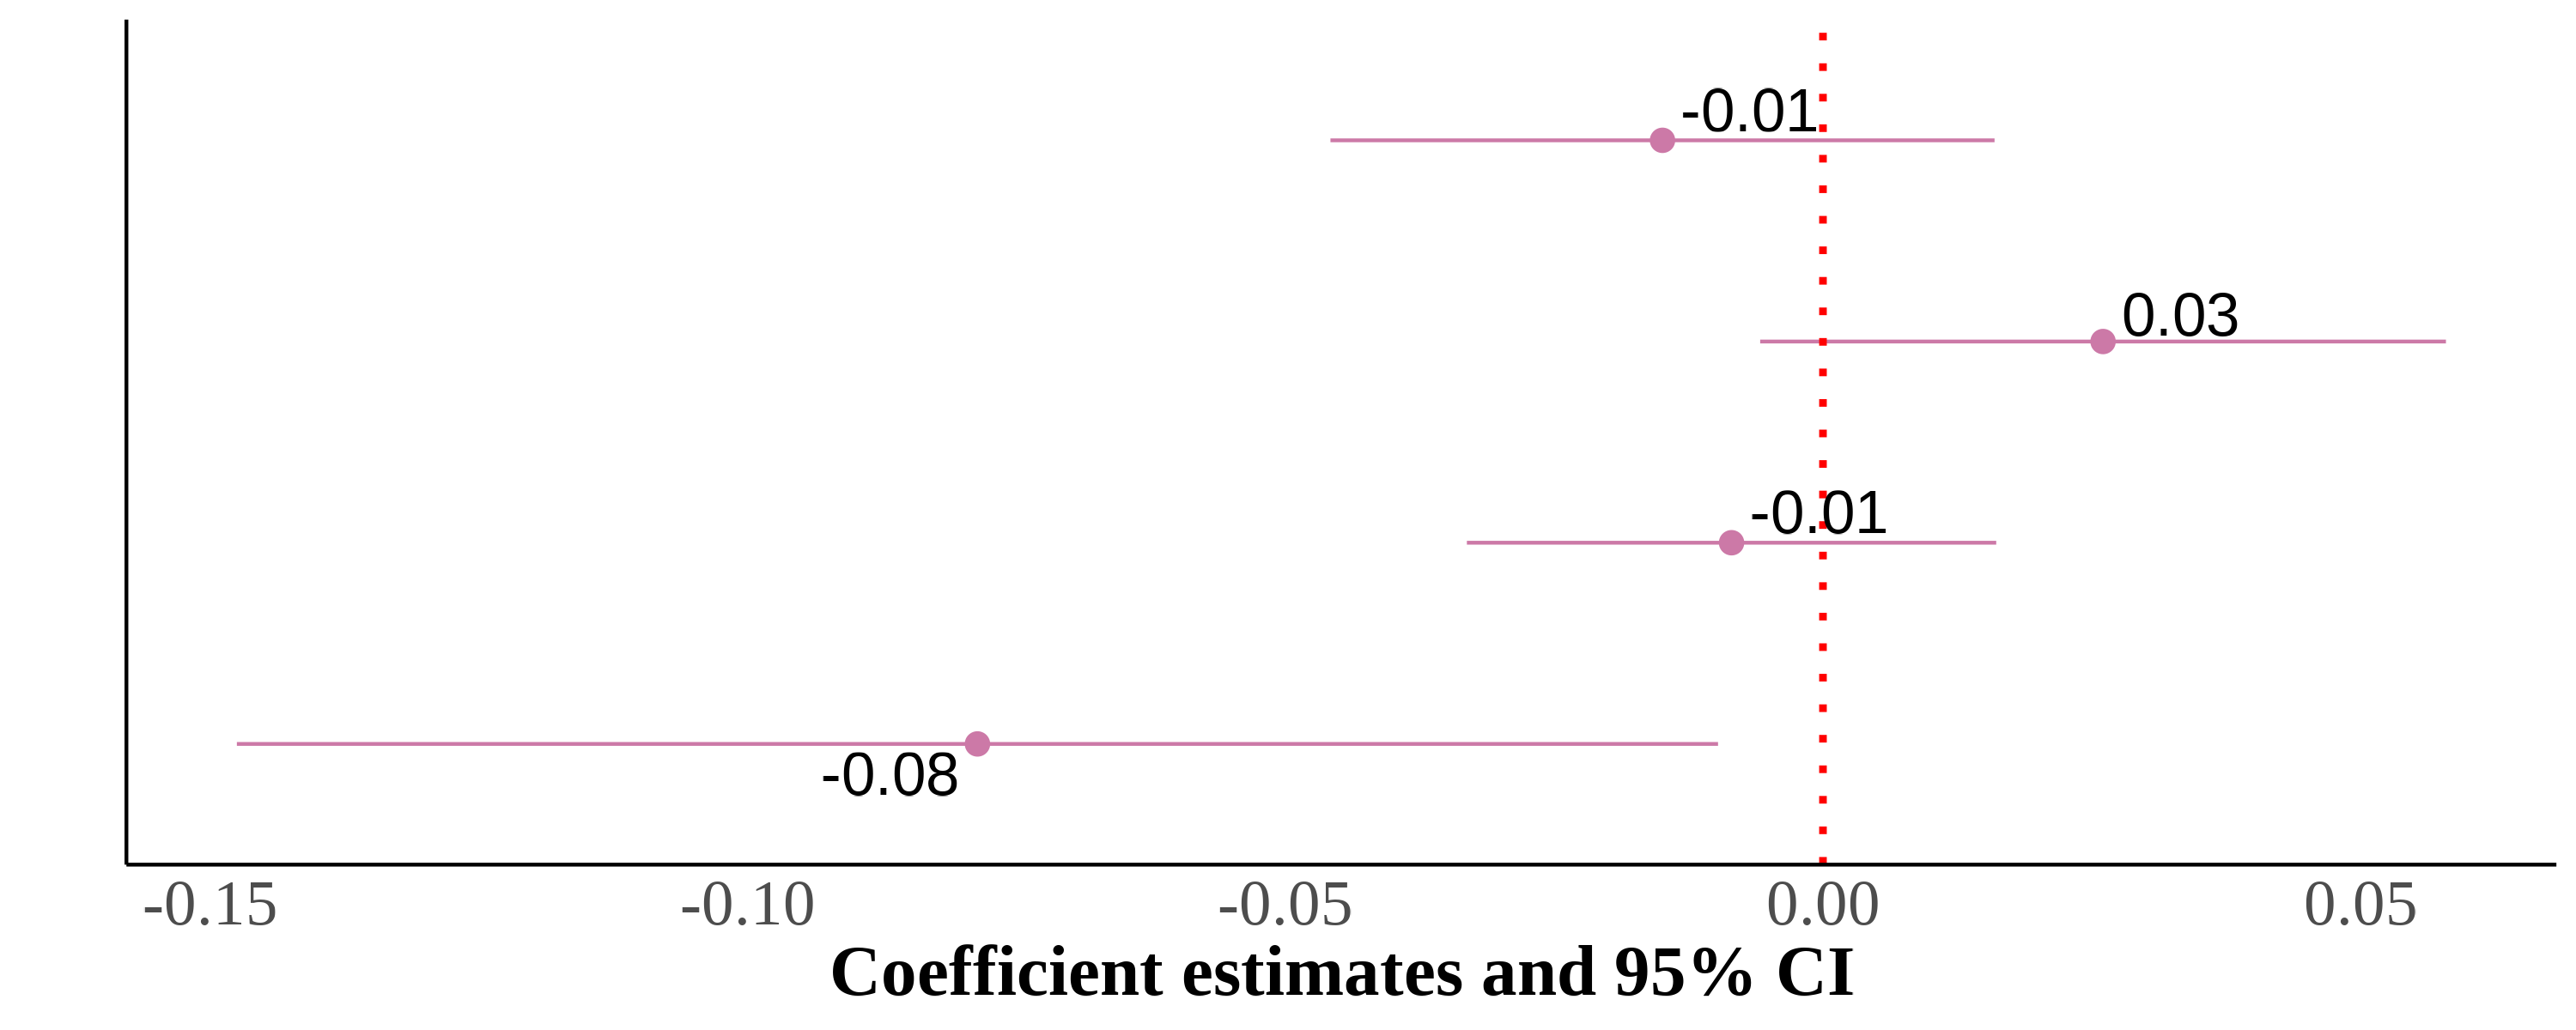
\includegraphics[width=.9\linewidth]{skin-iat-regression-third-gen.png}
\end{subfigure}
\caption*{\footnotesize{I show four panels of estimating equation (\ref{eq:identity_reg_bias}). I include region $\times$ year fixed effects with controls for sex, quartic age, and parental education. The dependent variable is self-reported Asian identity and the independent variable is state-level bias. Each panel is the results from the same regression but on different samples that are divided by generation. Standard errors are clustered on the state level. The samples include first-, second-, and third-generation Asian children ages 17 and below who live in intact families. First-generation Asian immigrants are children that were born in a Asian country. Native-born second-generation Asian immigrants are children with at least one parent born in a Asian country. Finally, native-born third-generation Asian immigrants are children with native-born parents and at least one grandparent born in a Asian country.}}
\end{figure}
\end{center}

\pagebreak
\newpage


\begin{center}
\begin{figure}[!htb]
\centering
\caption{Relationship Between Self-Reported Asian Identity and Bias: By Generation Among Adults}
\label{plot01-regression-gen-adults}
%First graph
\begin{subfigure}{.48\textwidth}
\caption{All Generations}
\centering
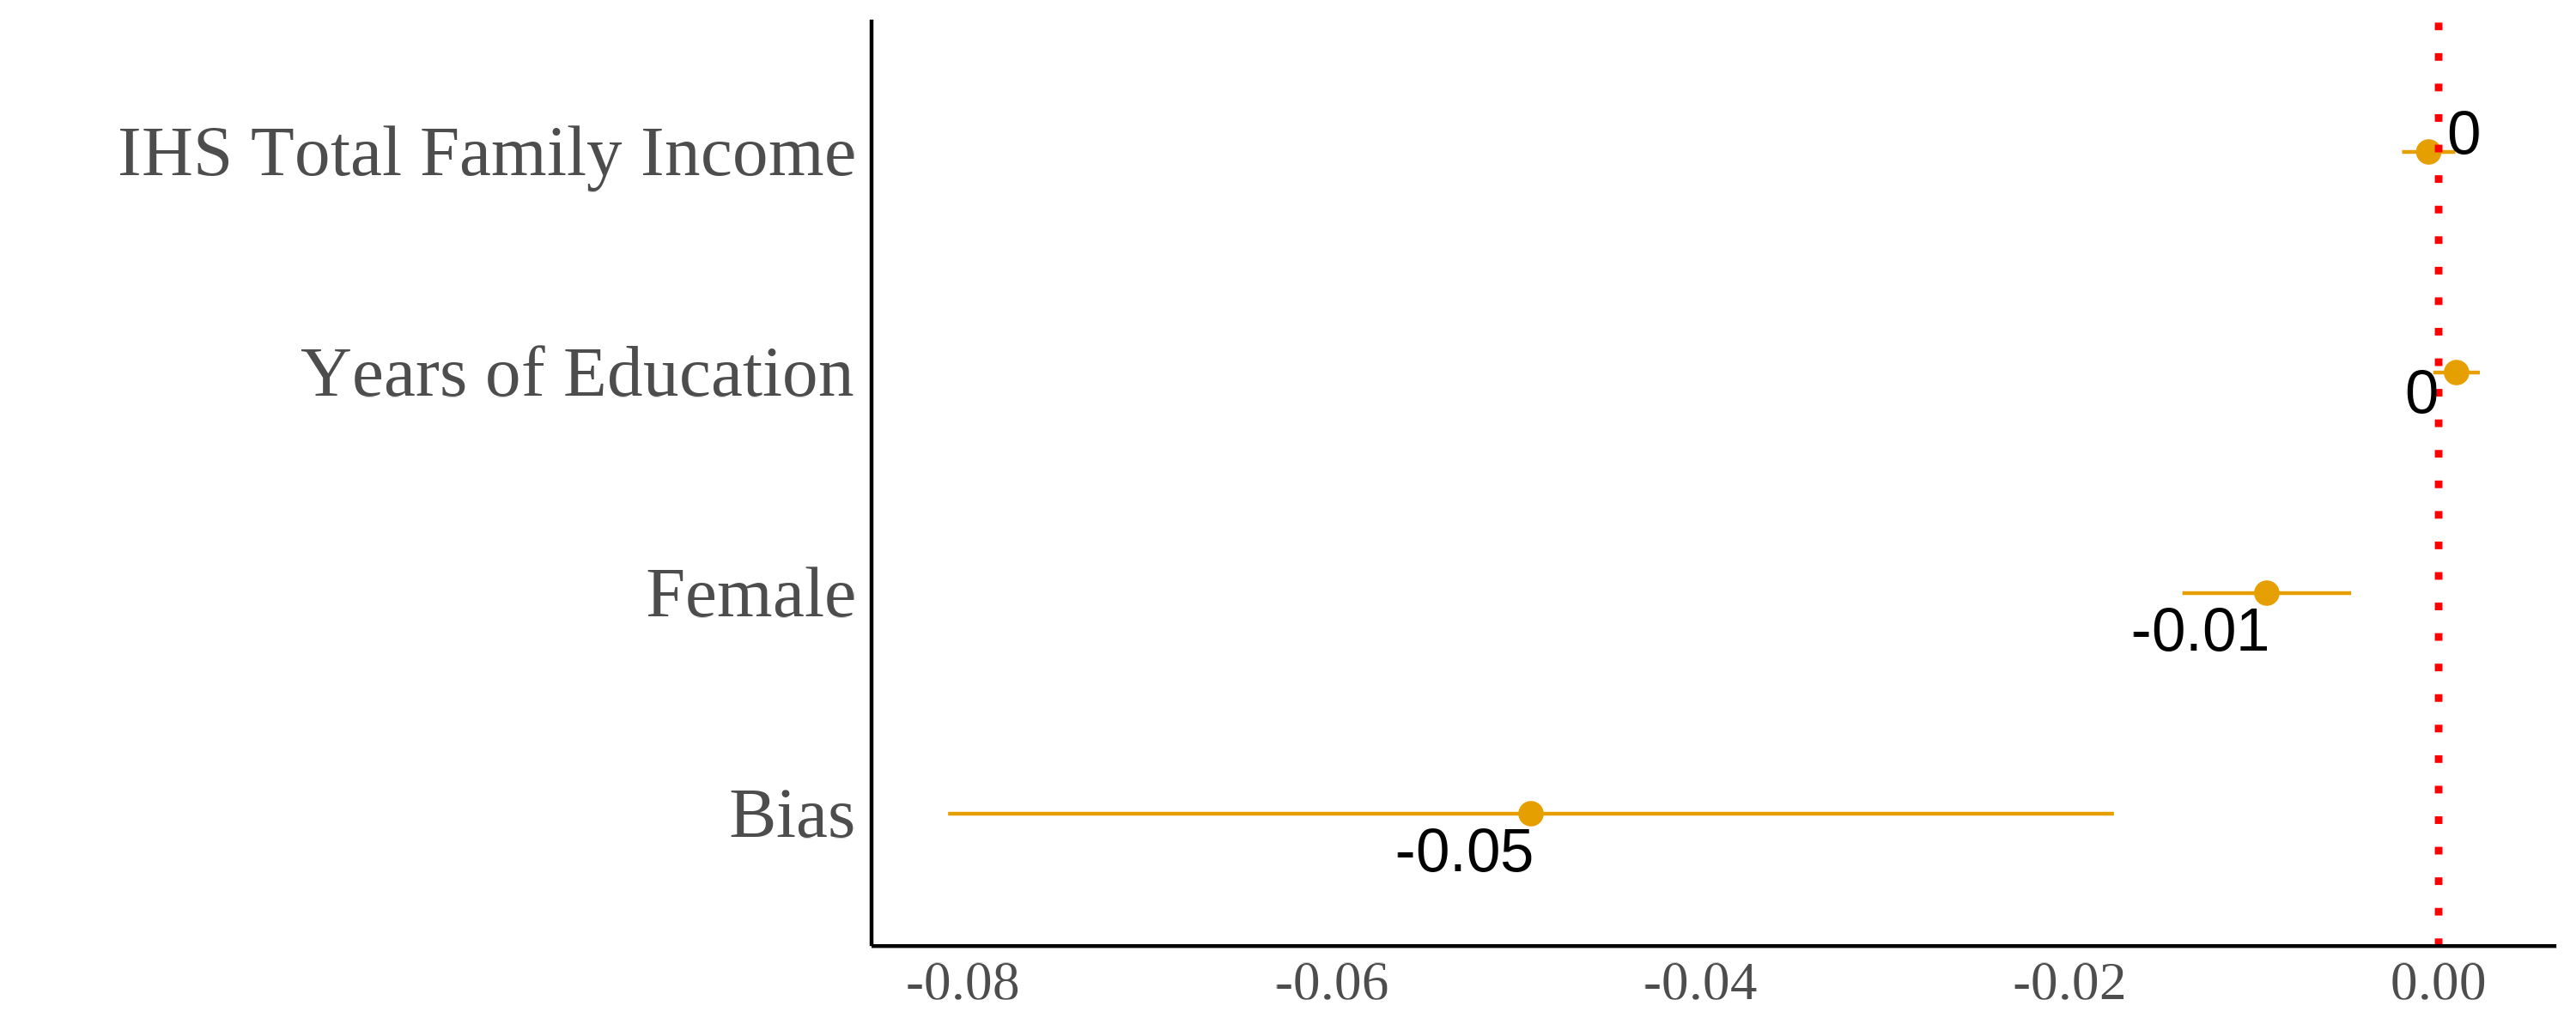
\includegraphics[width=.9\linewidth]{skin-iat-regression-all-gens-adults.png}
\end{subfigure}
\centering
%Second graph
\begin{subfigure}{.48\textwidth}
\caption{First-Generation}
\centering
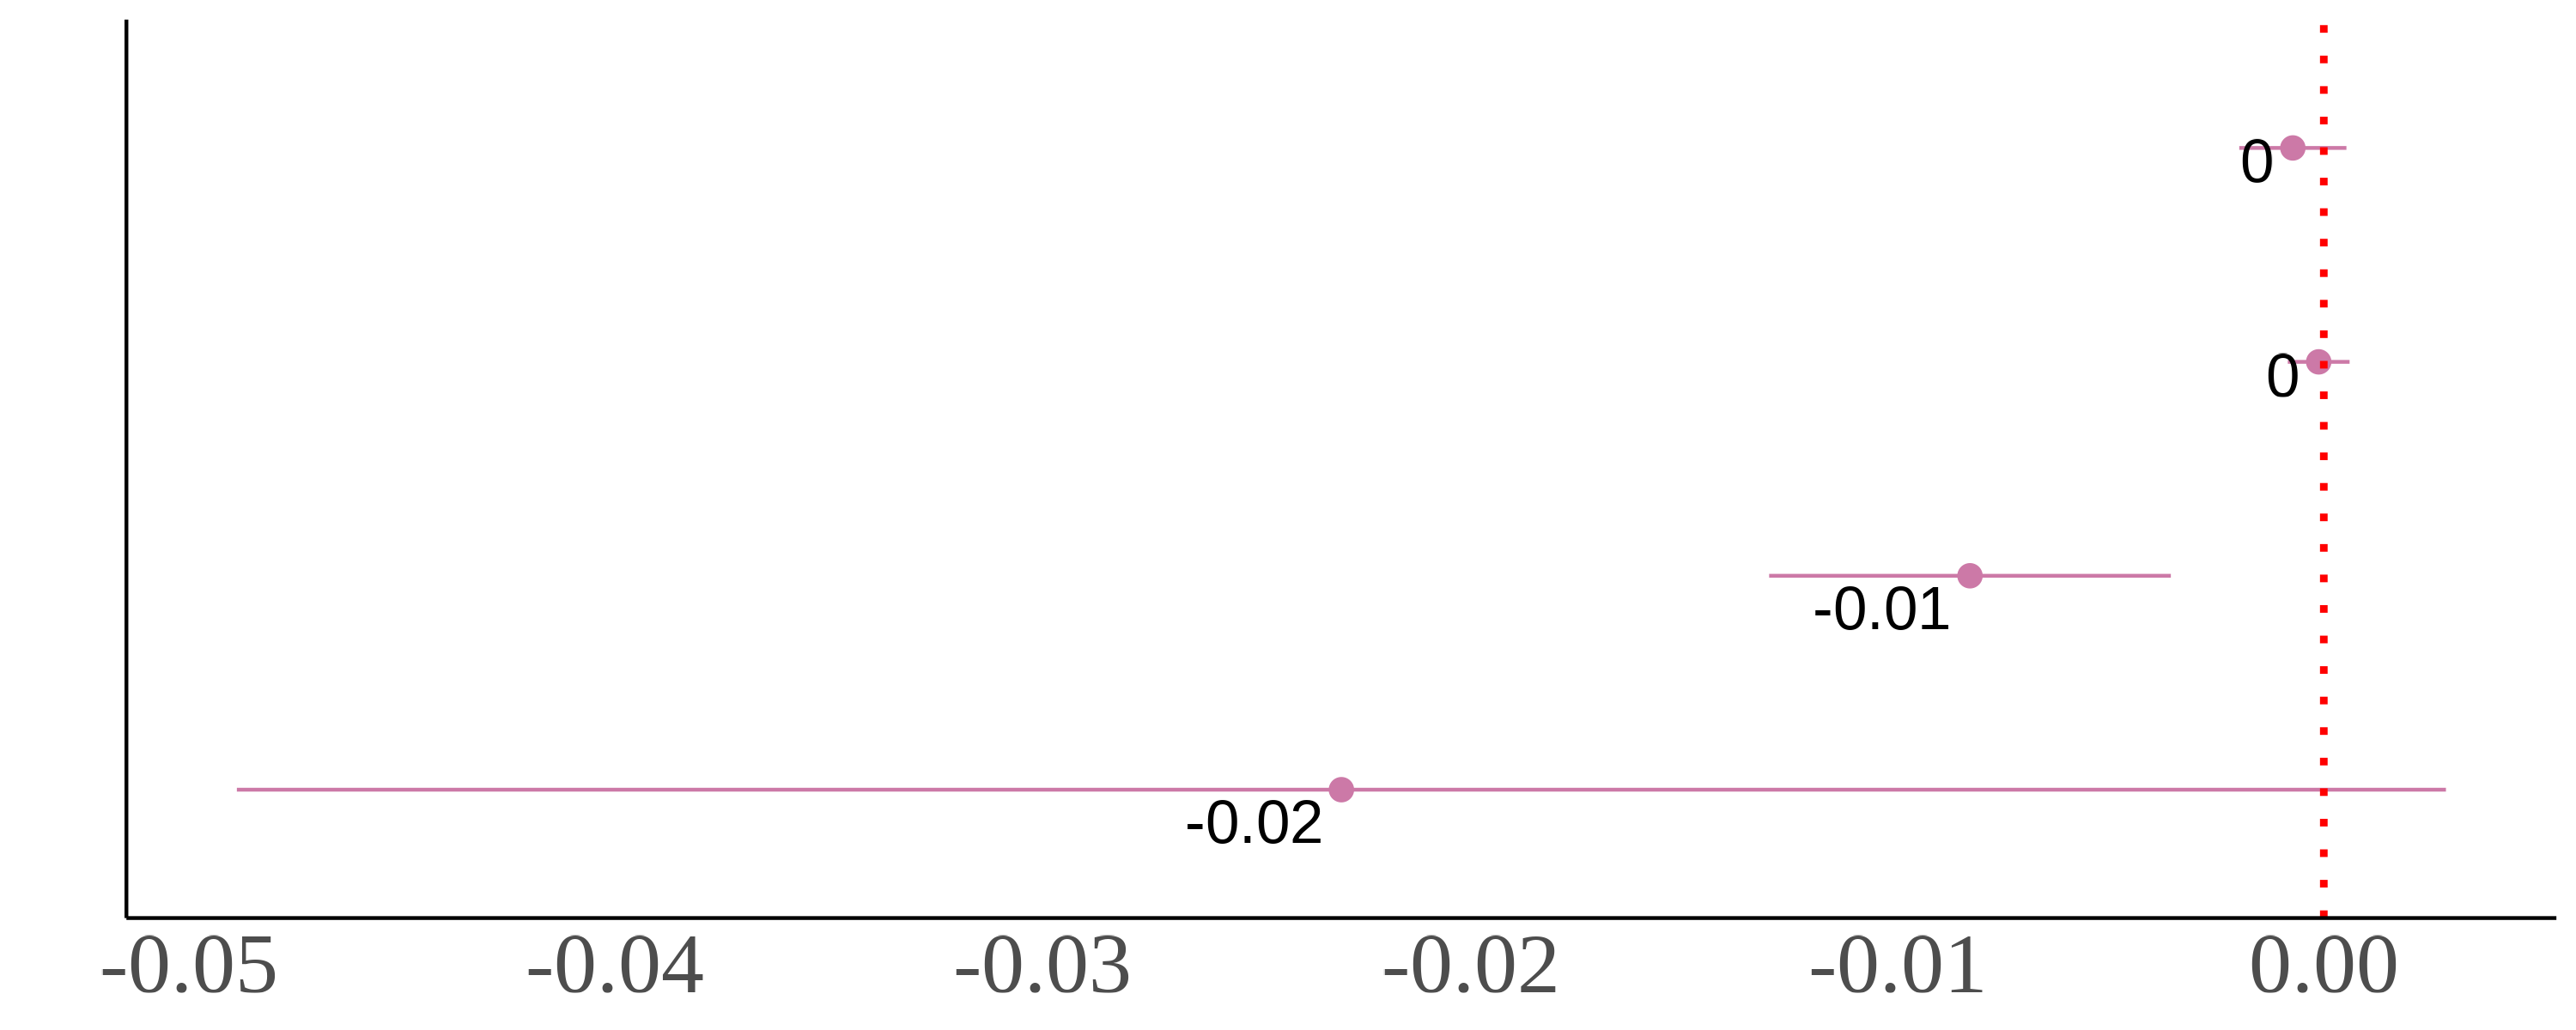
\includegraphics[width=.9\linewidth]{skin-iat-regression-first-gen-adults.png}
\end{subfigure}
%Third Graph
\begin{subfigure}{.48\textwidth}
\caption{Second-Generation}
\centering
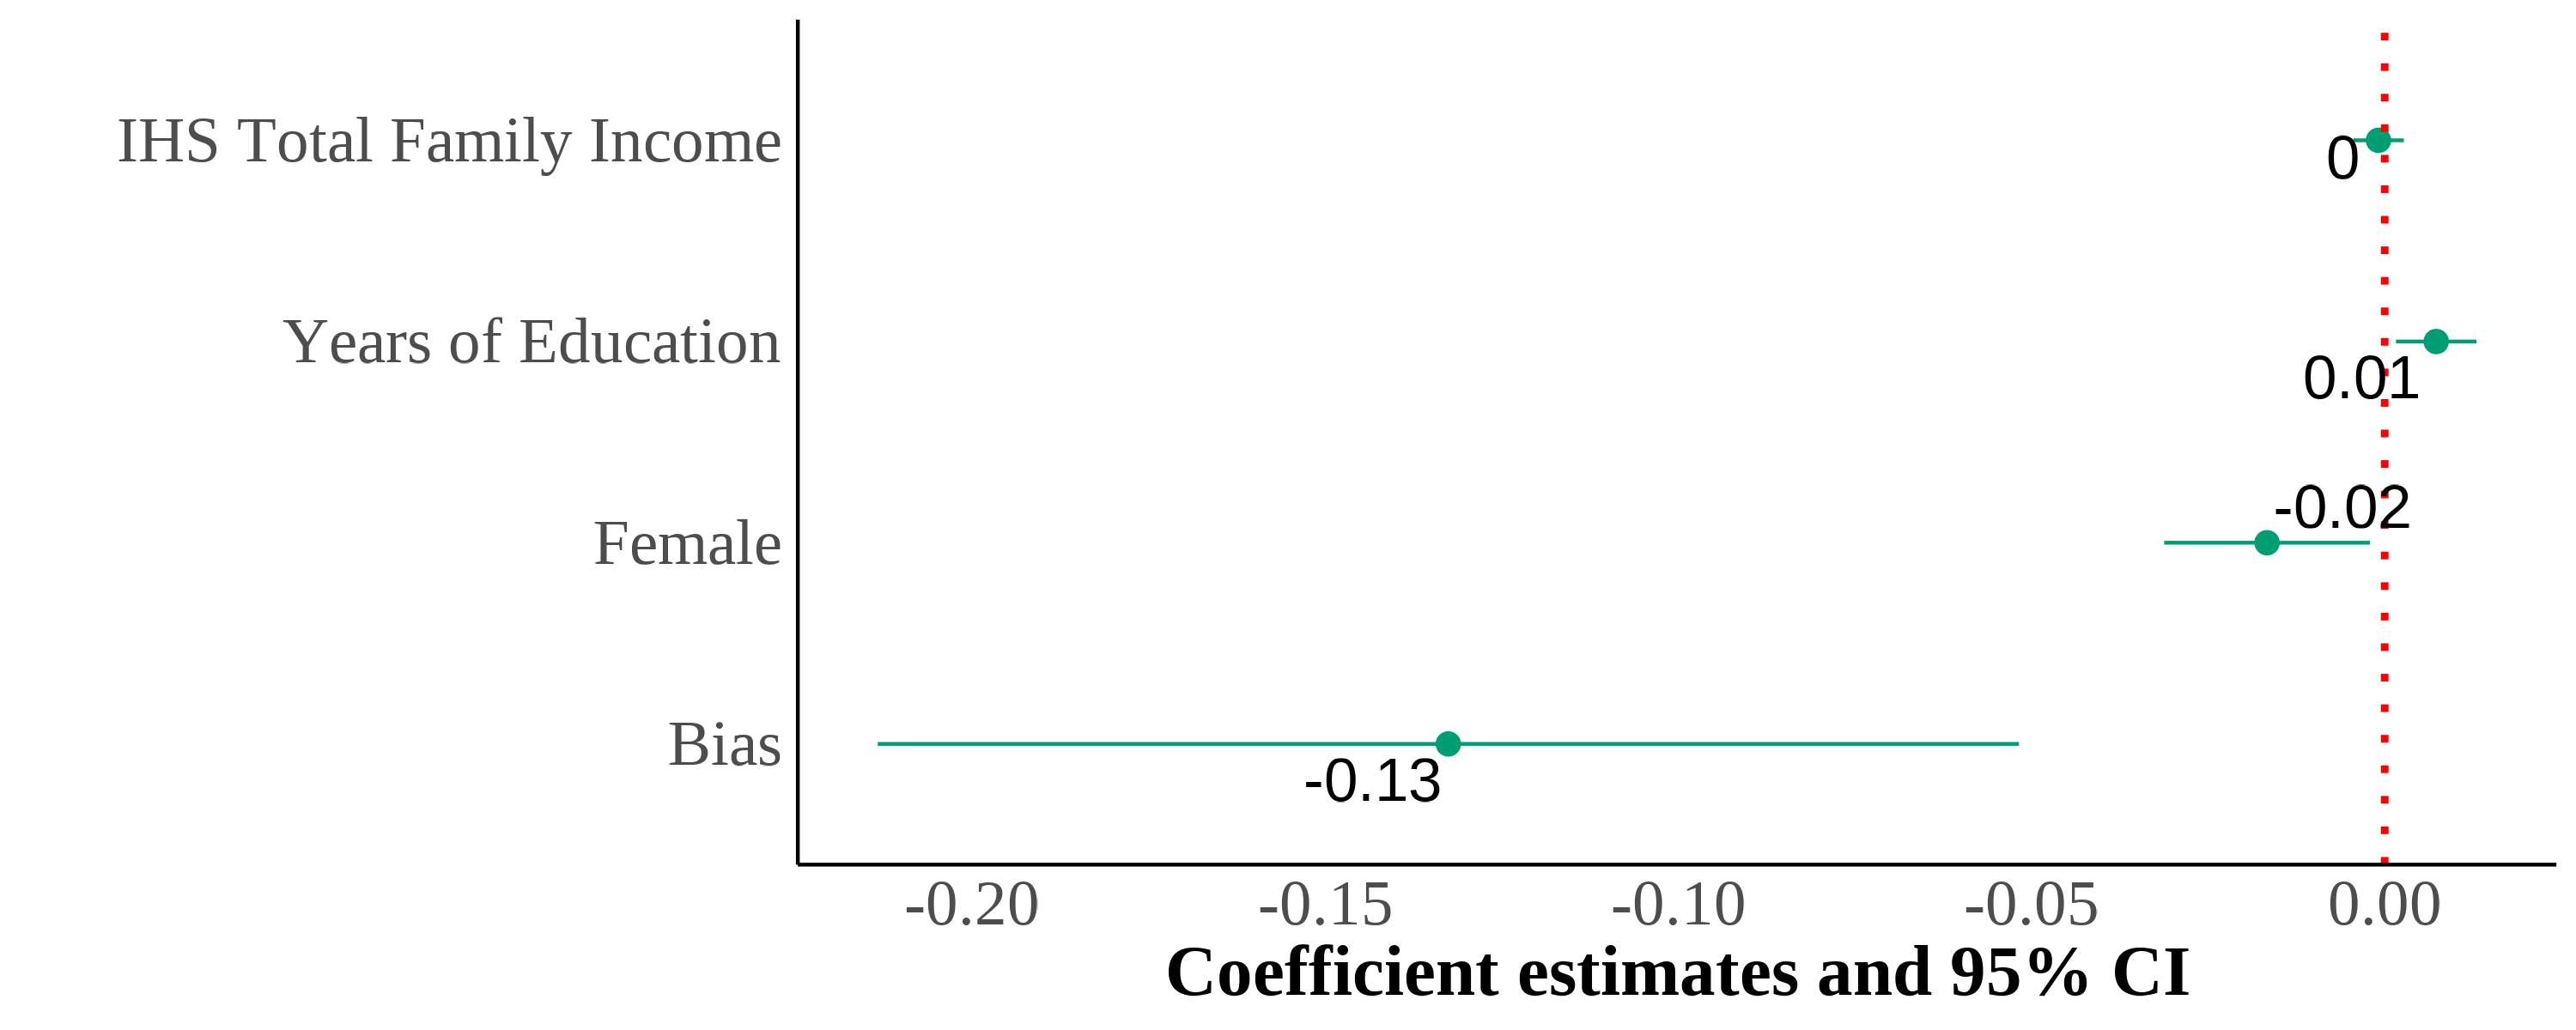
\includegraphics[width=.9\linewidth]{skin-iat-regression-second-gen-adults.png}
\end{subfigure}

\caption*{\footnotesize{I show three panels of estimating equation (\ref{eq:identity_reg_bias}) on a sample of adults. I include region $\times$ year fixed effects with controls for sex, quartic age, years of education, and inverse hyperbolic sine of income. The dependent variable is self-reported Asian identity and the independent variable is state-level bias. Each panel is the results from the same regression but on different samples that are divided by generation. Standard errors are clustered on the state level. The samples include first- and second-generation Asian adults ages 18 and above. First-generation Asian immigrants are individuals that were born in a Asian country. Native-born second-generation Asian immigrants are individuals with at least one parent born in a Asian country.}}
\end{figure}
\end{center}

\pagebreak
\newpage


\begin{center}
\begin{figure}[!htb]
\centering
\caption{Relationship Between Self-Reported Asian Identity and Bias: By Parental Types}
\label{plot01-regression-byparent}
%First graph
\begin{subfigure}{.48\textwidth}
\caption{Second-Generation (All Parental Types)}
\centering
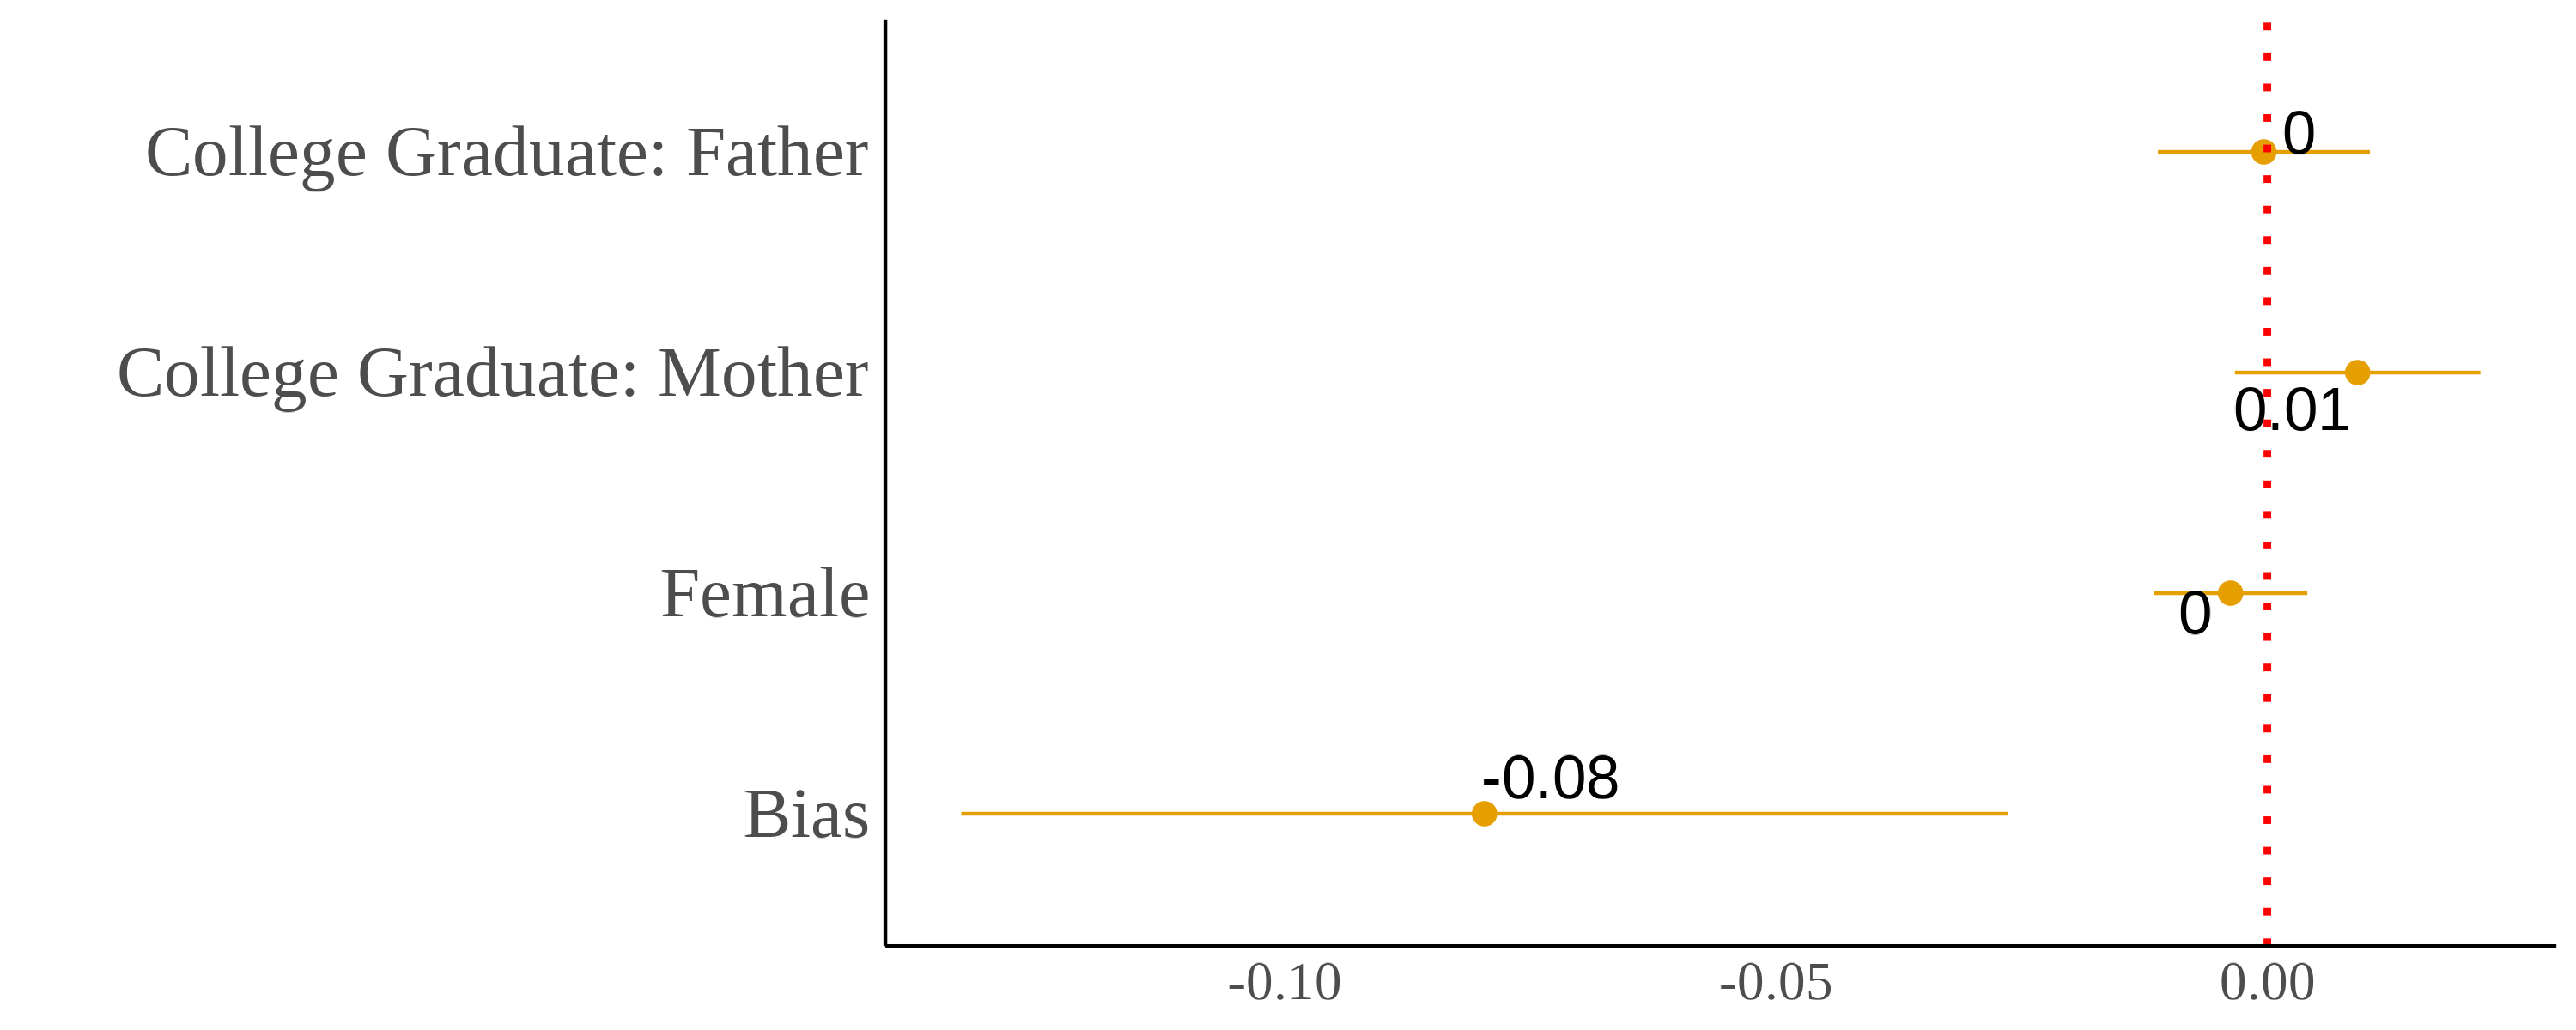
\includegraphics[width=.9\linewidth]{by-parents-regs-all.png}
\end{subfigure}
\centering
%Second graph
\begin{subfigure}{.48\textwidth}
\caption{Asian Fathers-Asian Mothers}
\centering
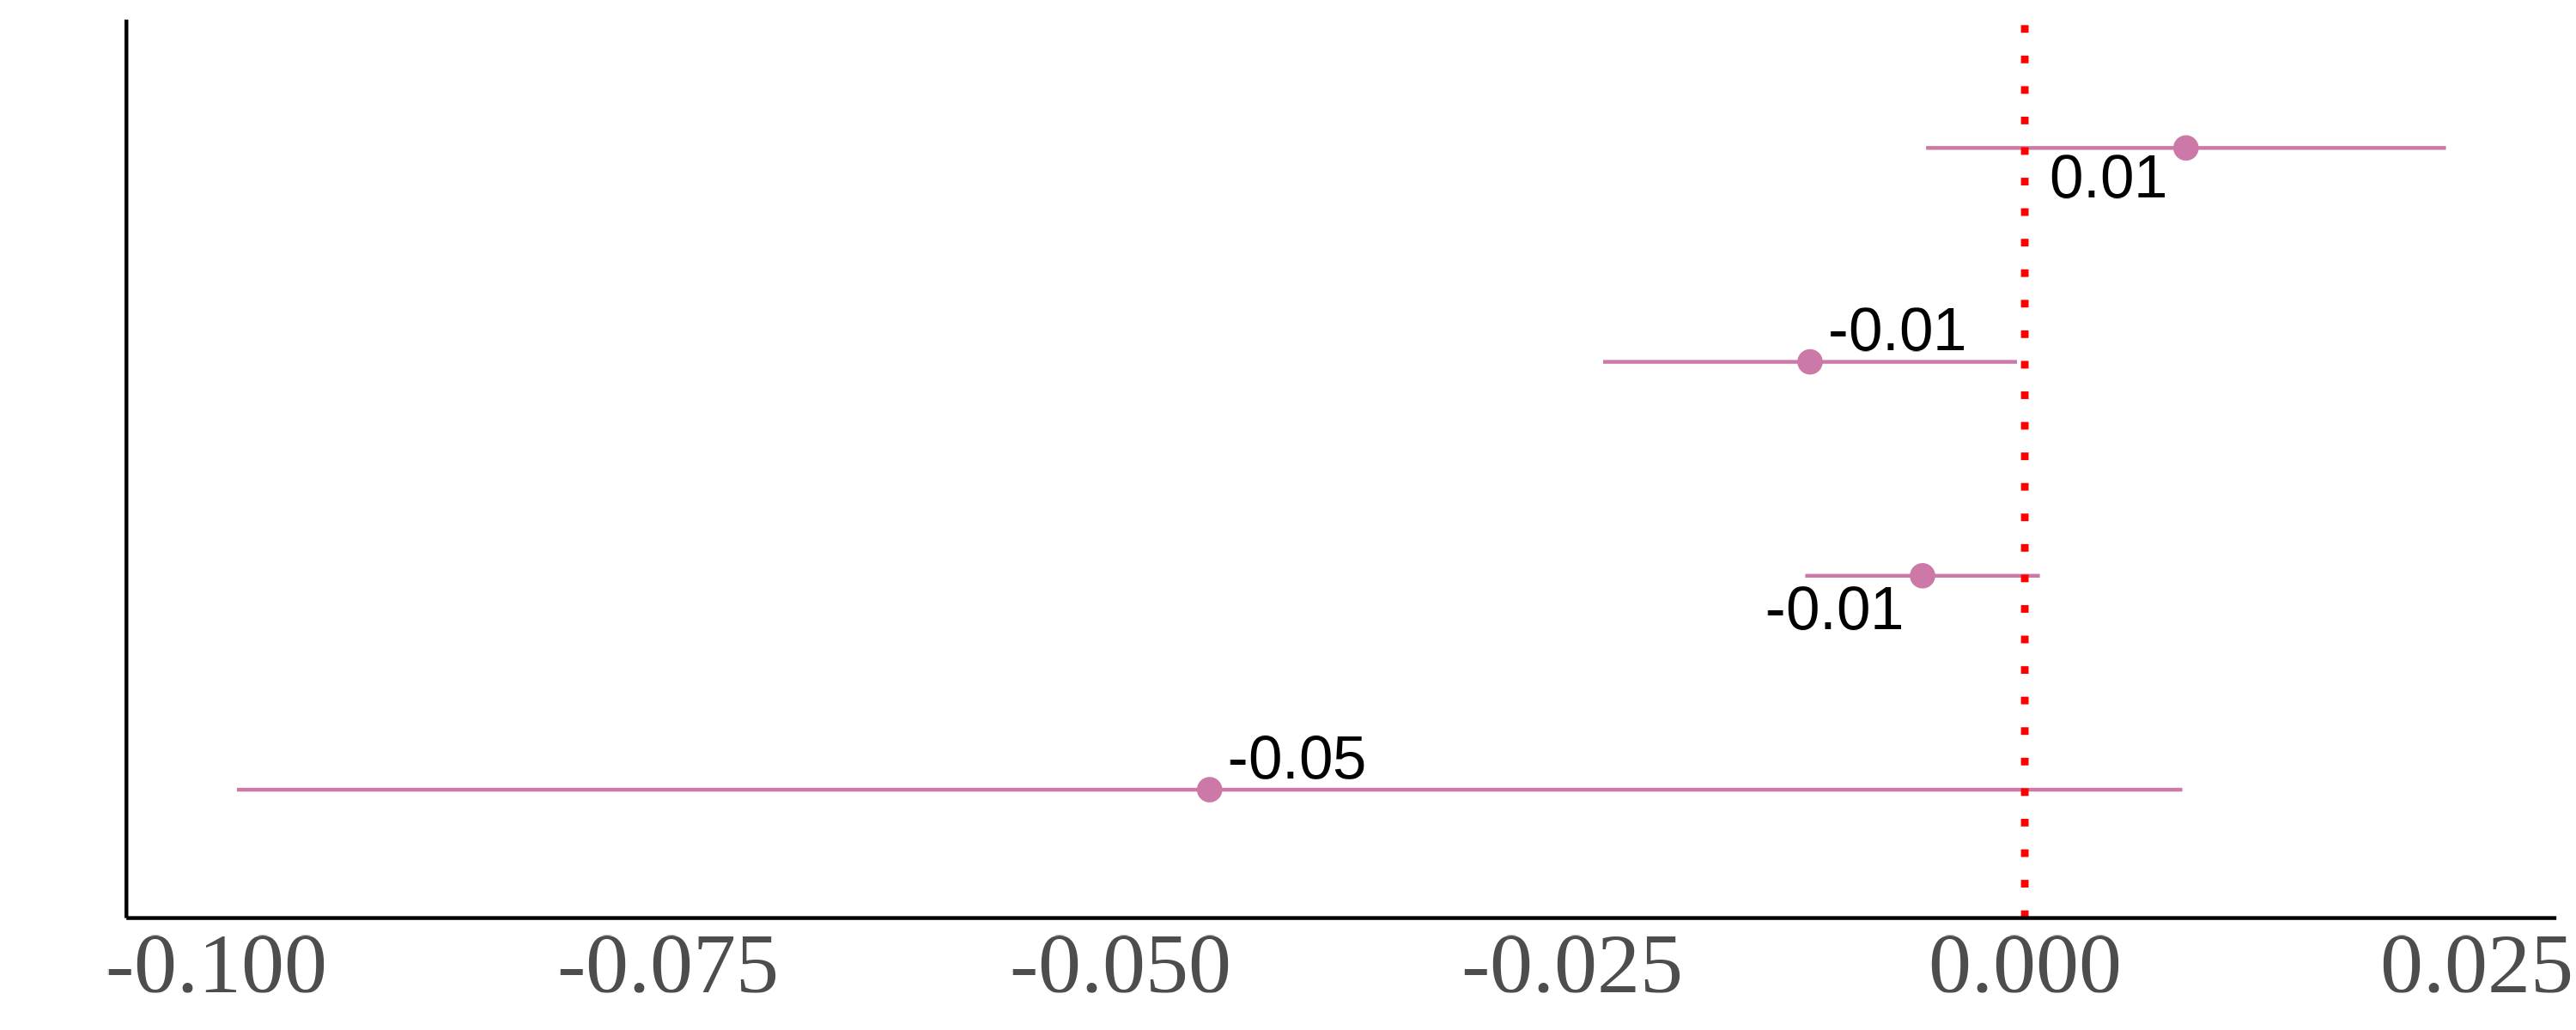
\includegraphics[width=.9\linewidth]{by-parents-regs-hh.png}
\end{subfigure}
%Third Graph
\begin{subfigure}{.48\textwidth}
\caption{Asian Fathers-White Mothers}
\centering
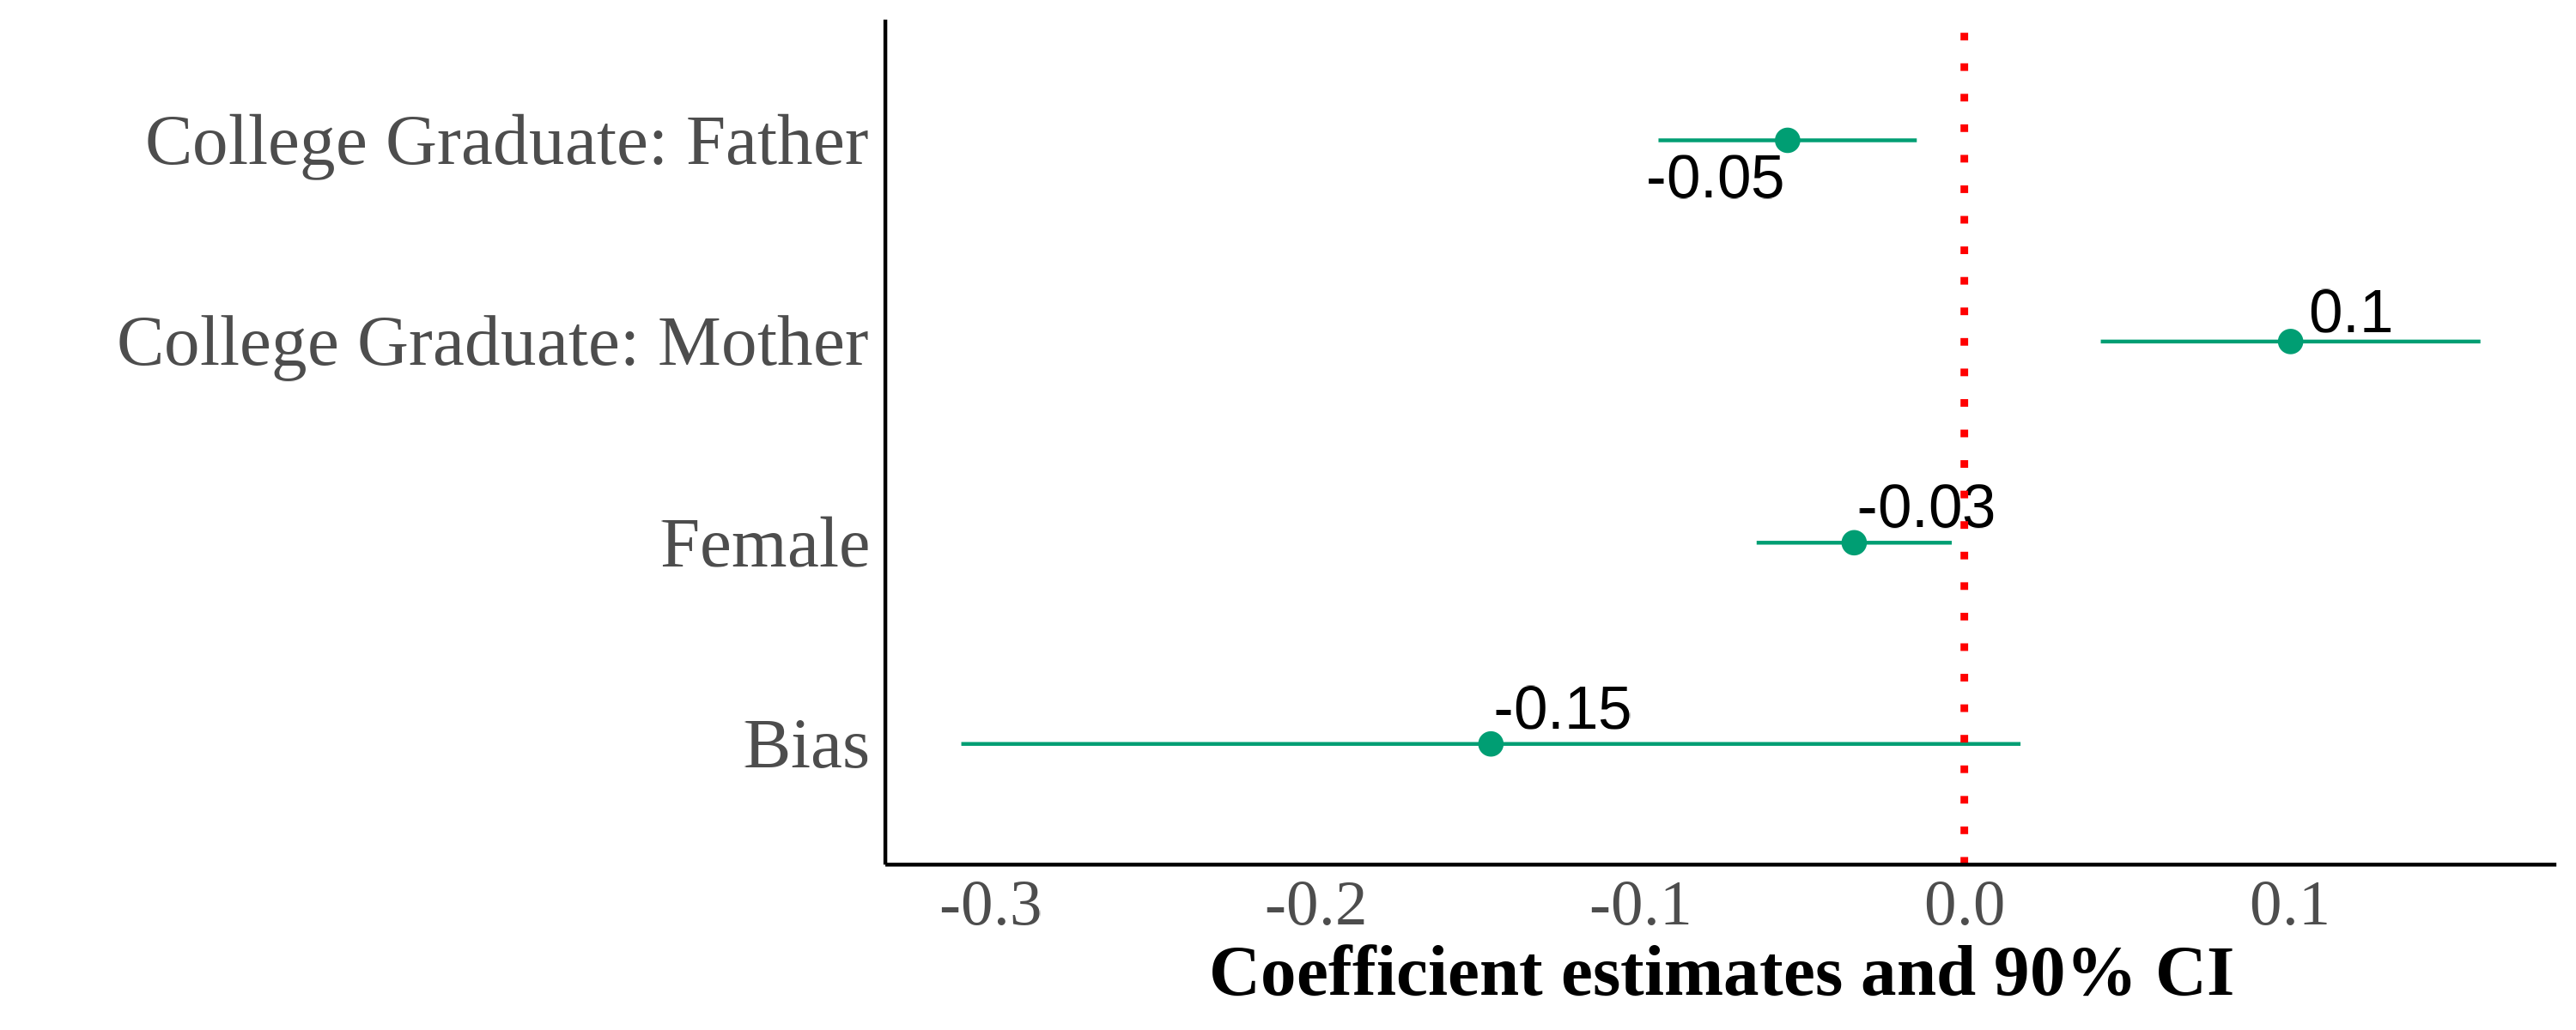
\includegraphics[width=.9\linewidth]{by-parents-regs-hw.png}
\end{subfigure}
%Fourth Graph
\begin{subfigure}{.48\textwidth}
\caption{White Fathers-Asian Mothers}
\centering
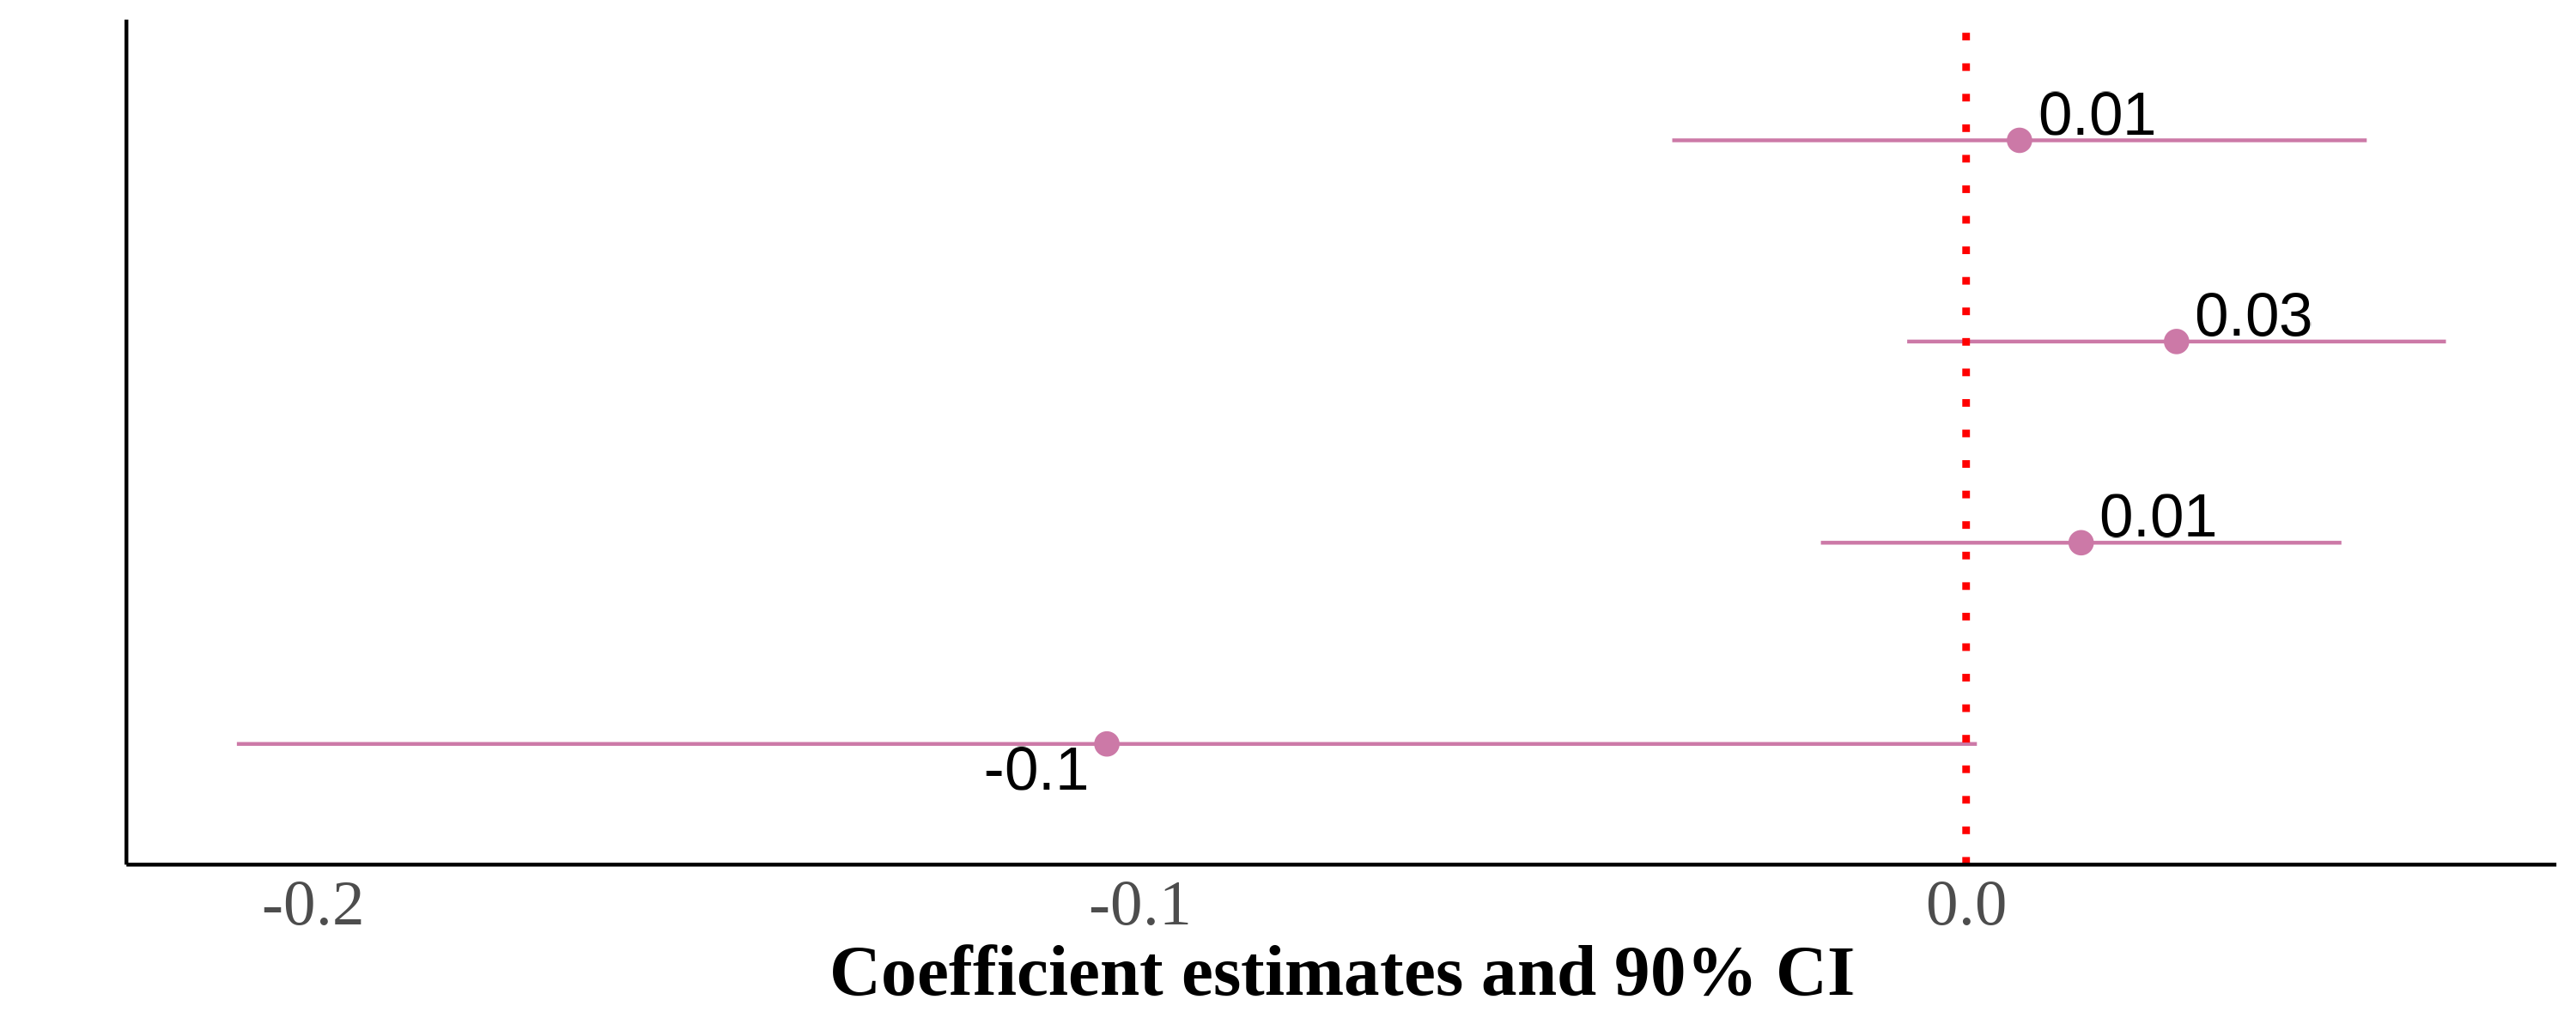
\includegraphics[width=.9\linewidth]{by-parents-regs-wh.png}
\end{subfigure}
\caption*{\footnotesize{I show four panels of estimating equation (\ref{eq:identity_reg_bias}). I include region $\times$ year fixed effects with controls for sex, quartic age, and parental education. The dependent variable is self-reported Asian identity and the independent variable is state-level bias. Each panel results from the same regression but on different samples divided by parental types. Standard errors are clustered on the state level. The samples include second-generation Asian children ages 17 and below who live in intact families. Native-born second-generation Asian immigrant children with at least one parent born in an Asian country.}}
\end{figure}
\end{center}

\pagebreak
\newpage

\begin{center}
\begin{figure}[!htb]
\centering
\caption{Relationship Between Self-Reported Asian Identity and Bias: By Parental Types Among Adults}
\label{plot01-regression-byparent-adults}
%First graph
\begin{subfigure}{.48\textwidth}
\caption{Second-Generation (All Parental Types)}
\centering
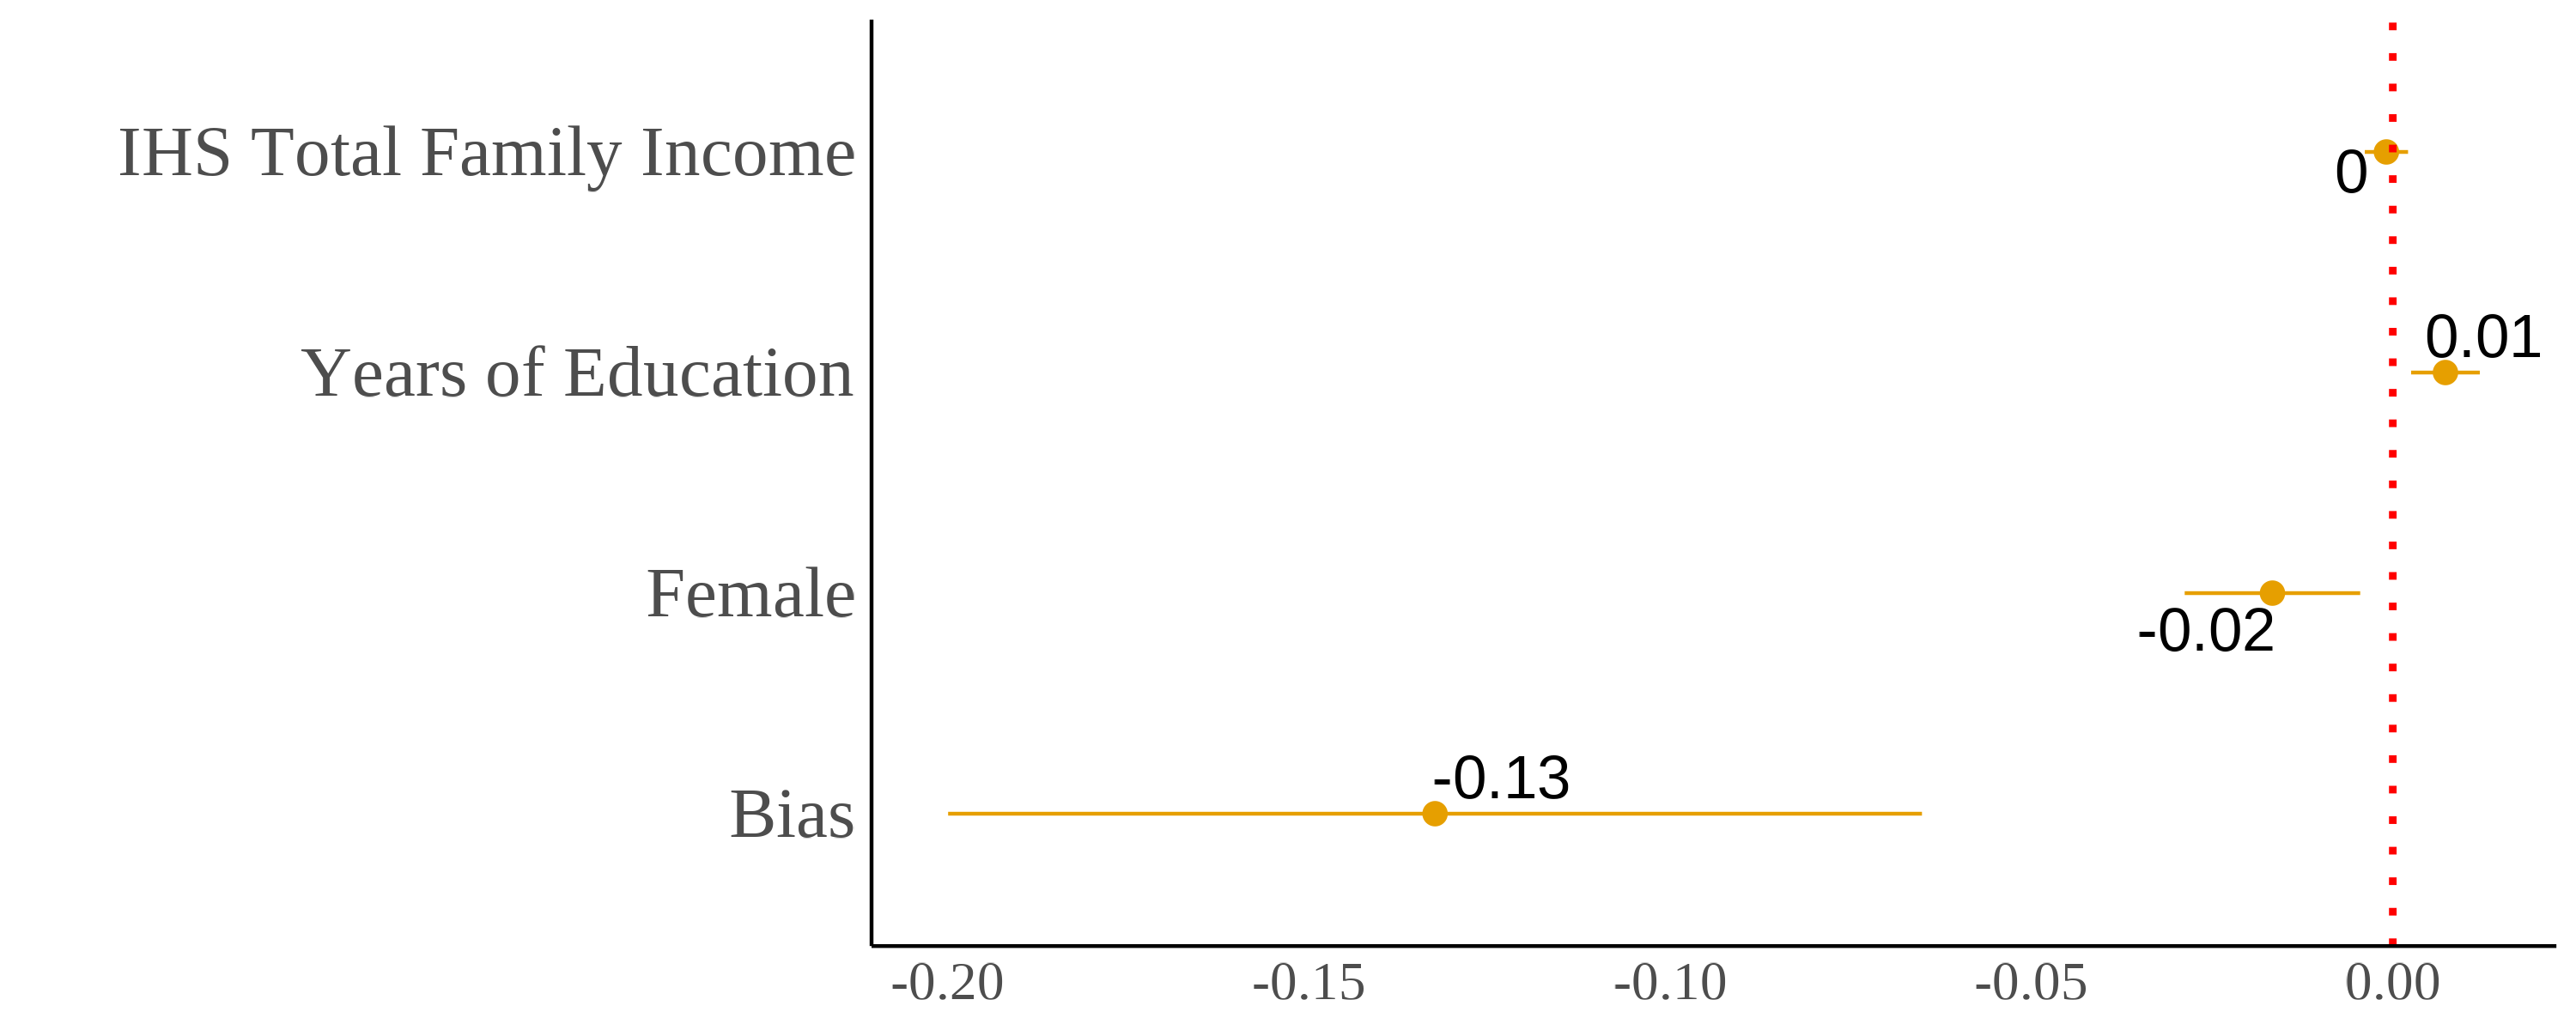
\includegraphics[width=.9\linewidth]{by-parents-regs-all-adults.png}
\end{subfigure}
\centering
%Second graph
\begin{subfigure}{.48\textwidth}
\caption{Asian Fathers-Asian Mothers}
\centering
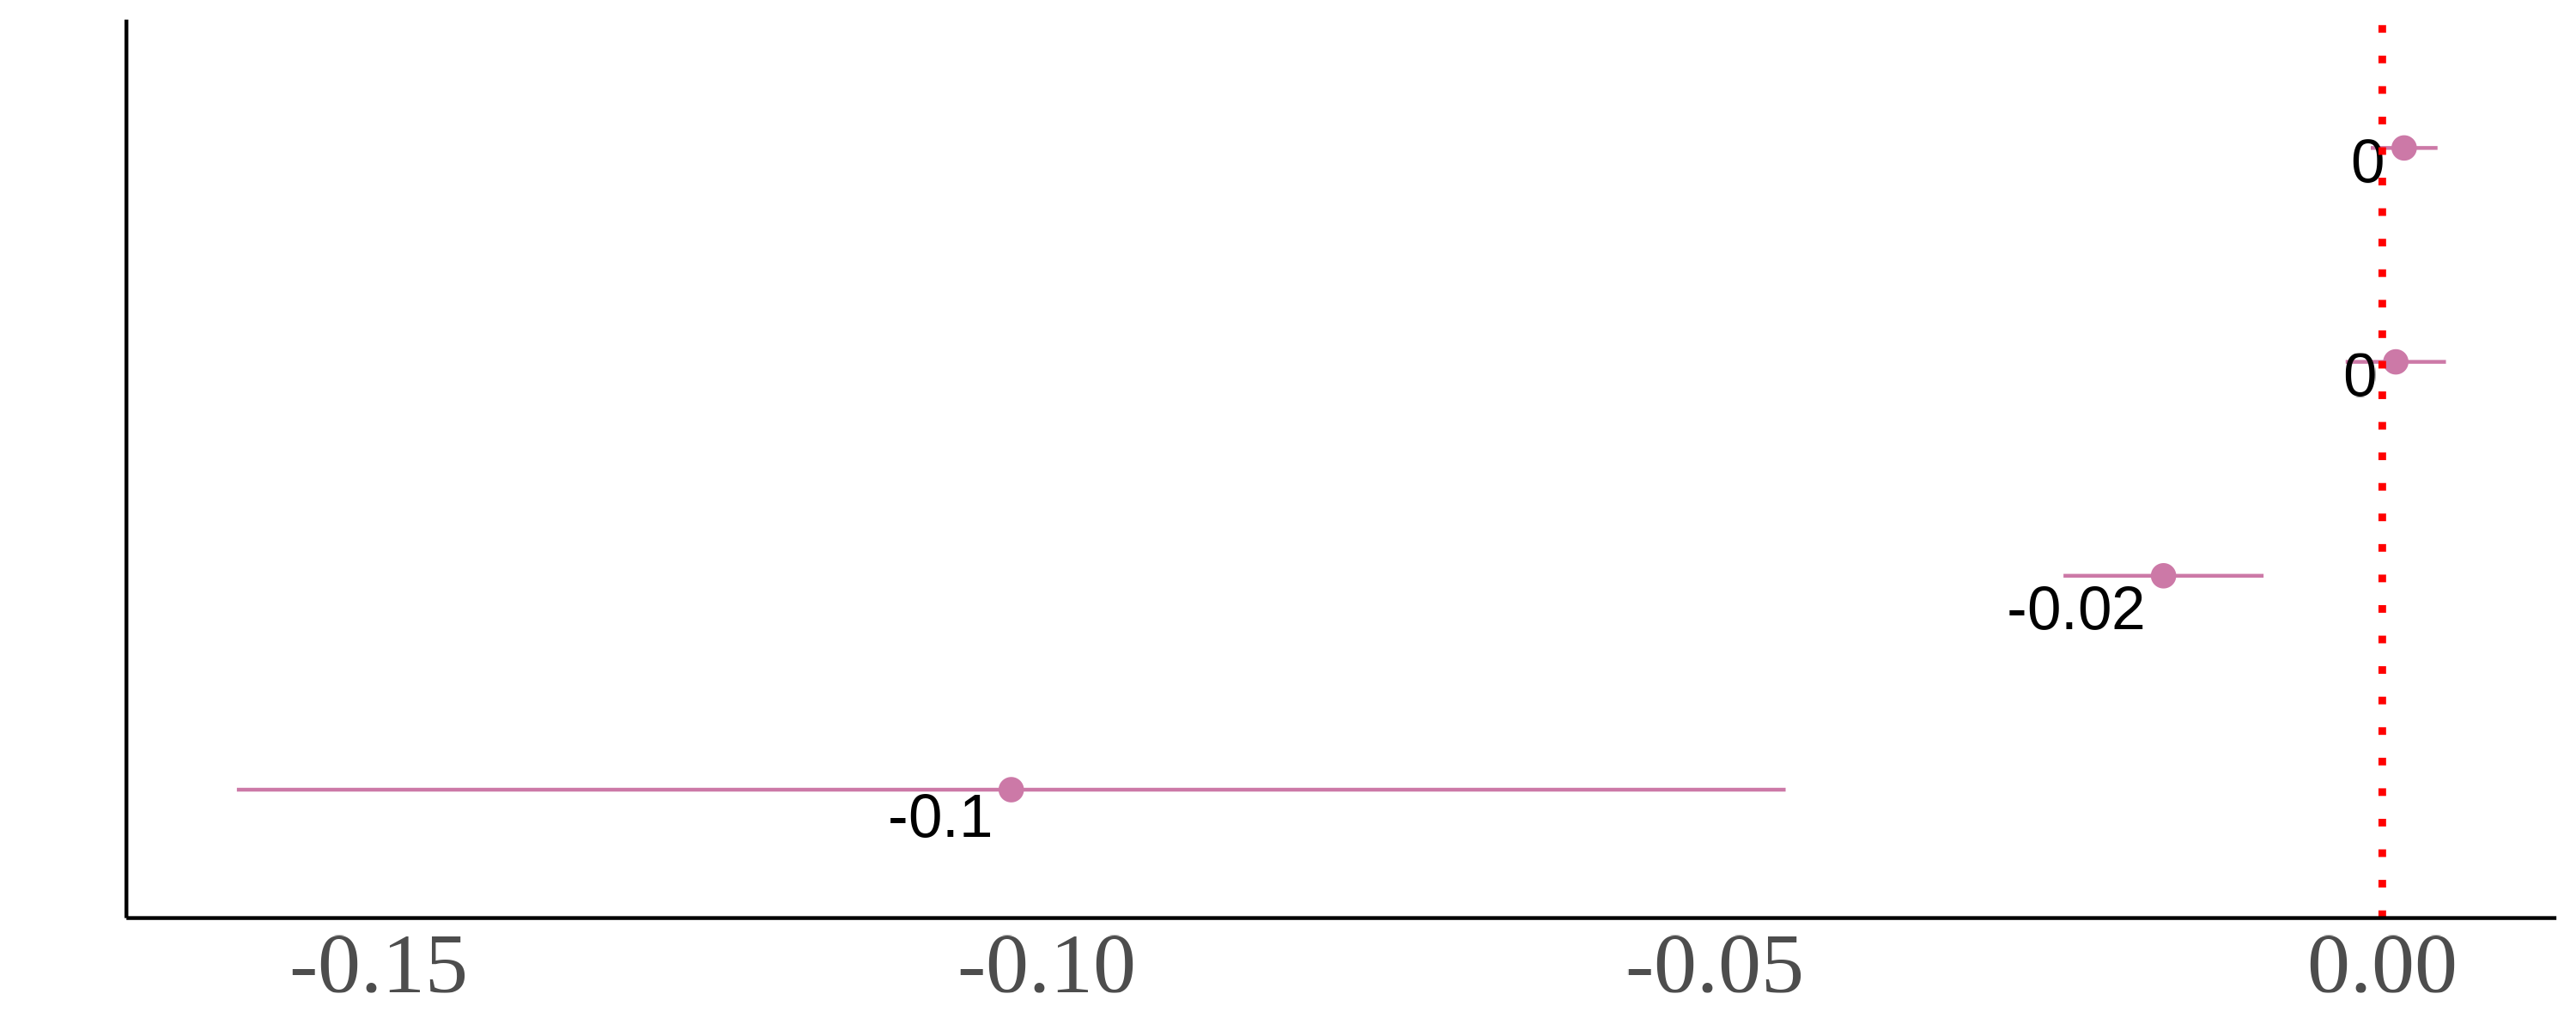
\includegraphics[width=.9\linewidth]{by-parents-regs-hh-adults.png}
\end{subfigure}
%Third Graph
\begin{subfigure}{.48\textwidth}
\caption{Asian Fathers-White Mothers}
\centering
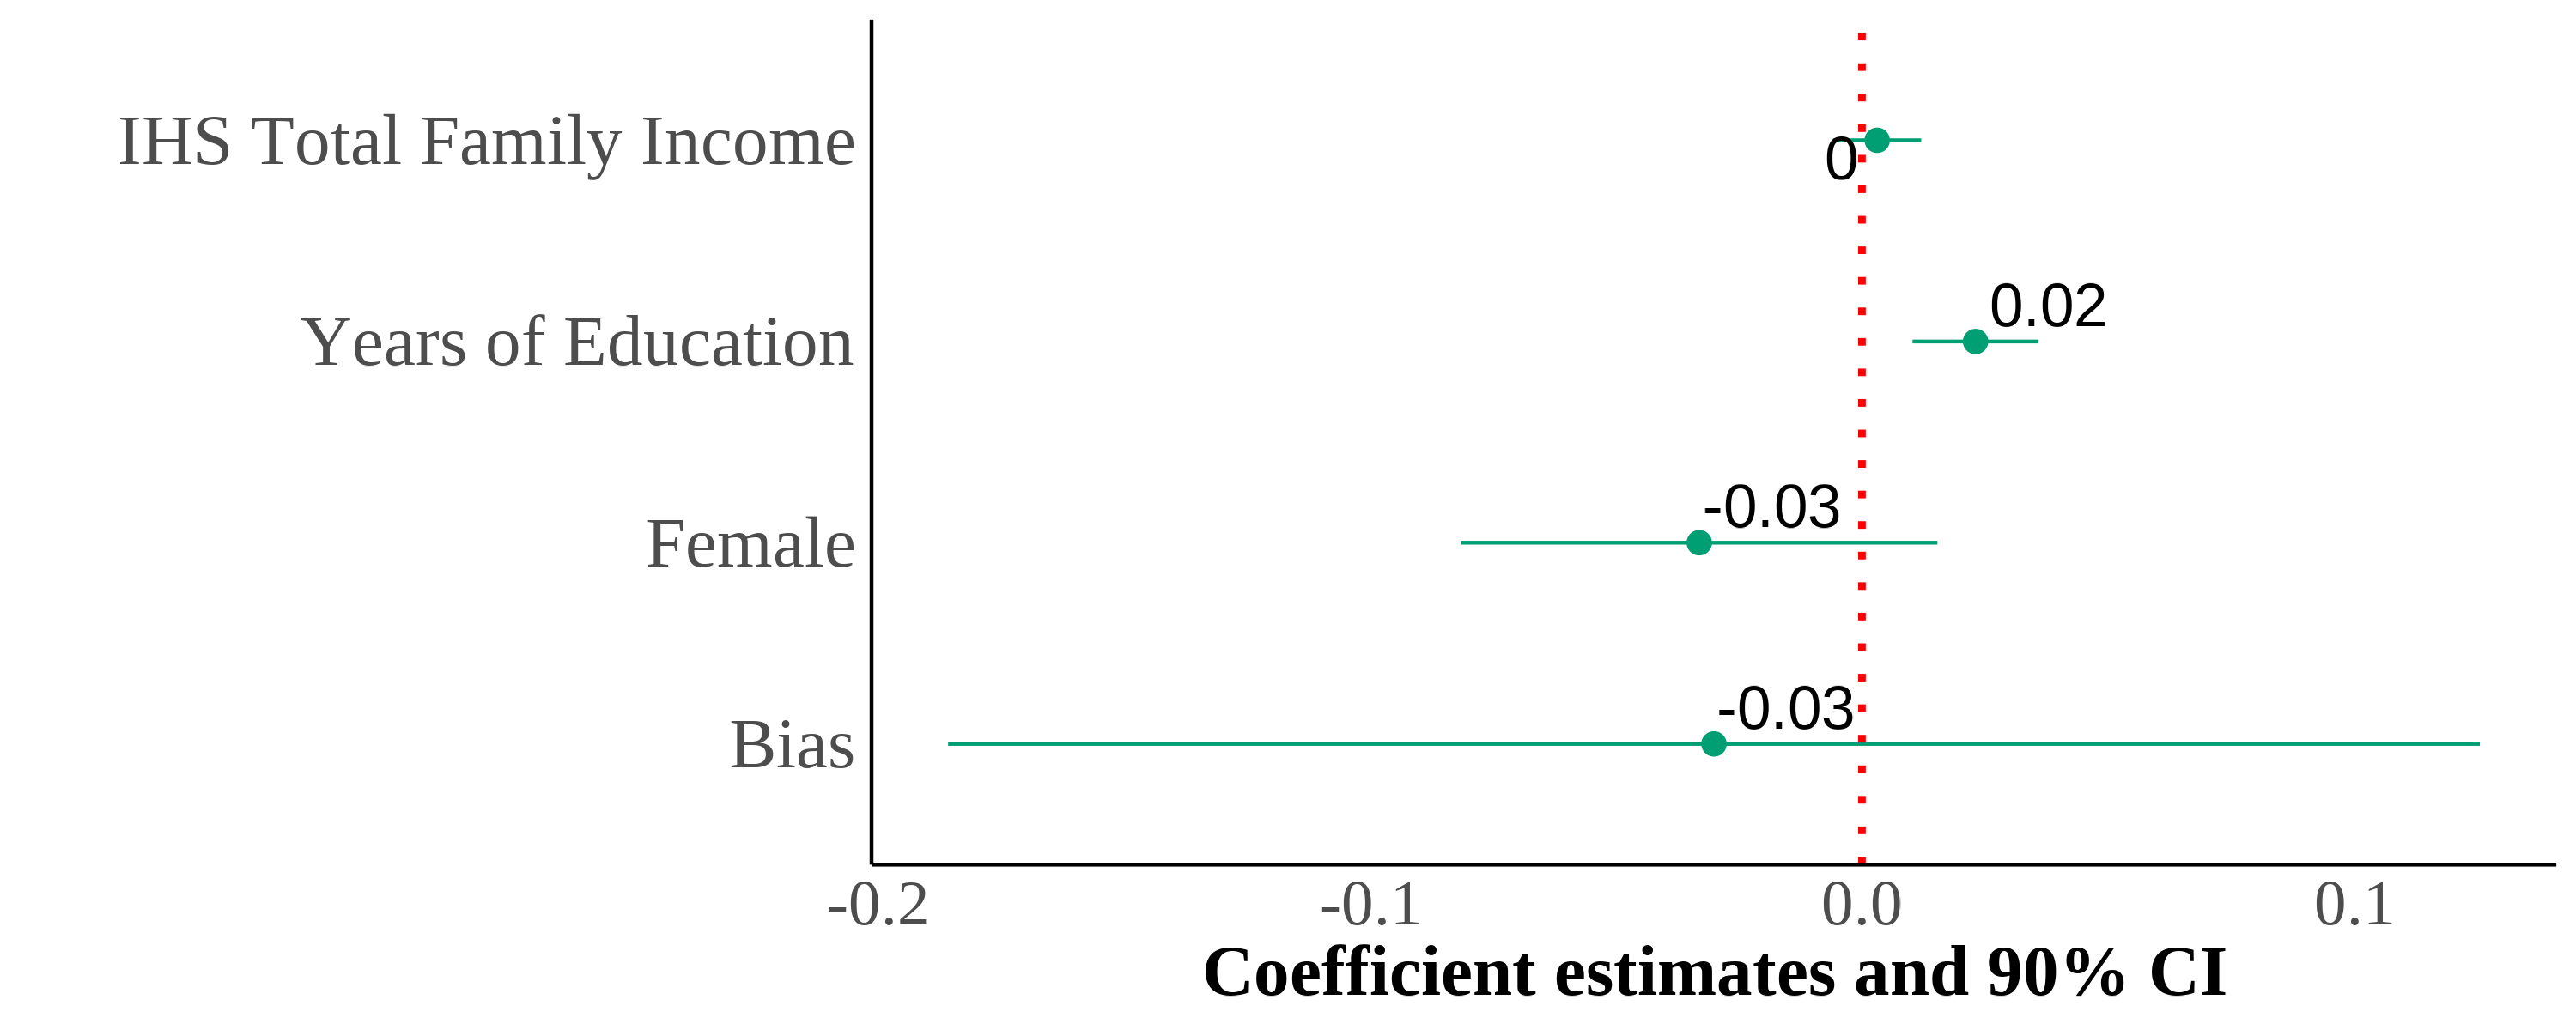
\includegraphics[width=.9\linewidth]{by-parents-regs-hw-adults.png}
\end{subfigure}
%Fourth Graph
\begin{subfigure}{.48\textwidth}
\caption{White Fathers-Asian Mothers}
\centering
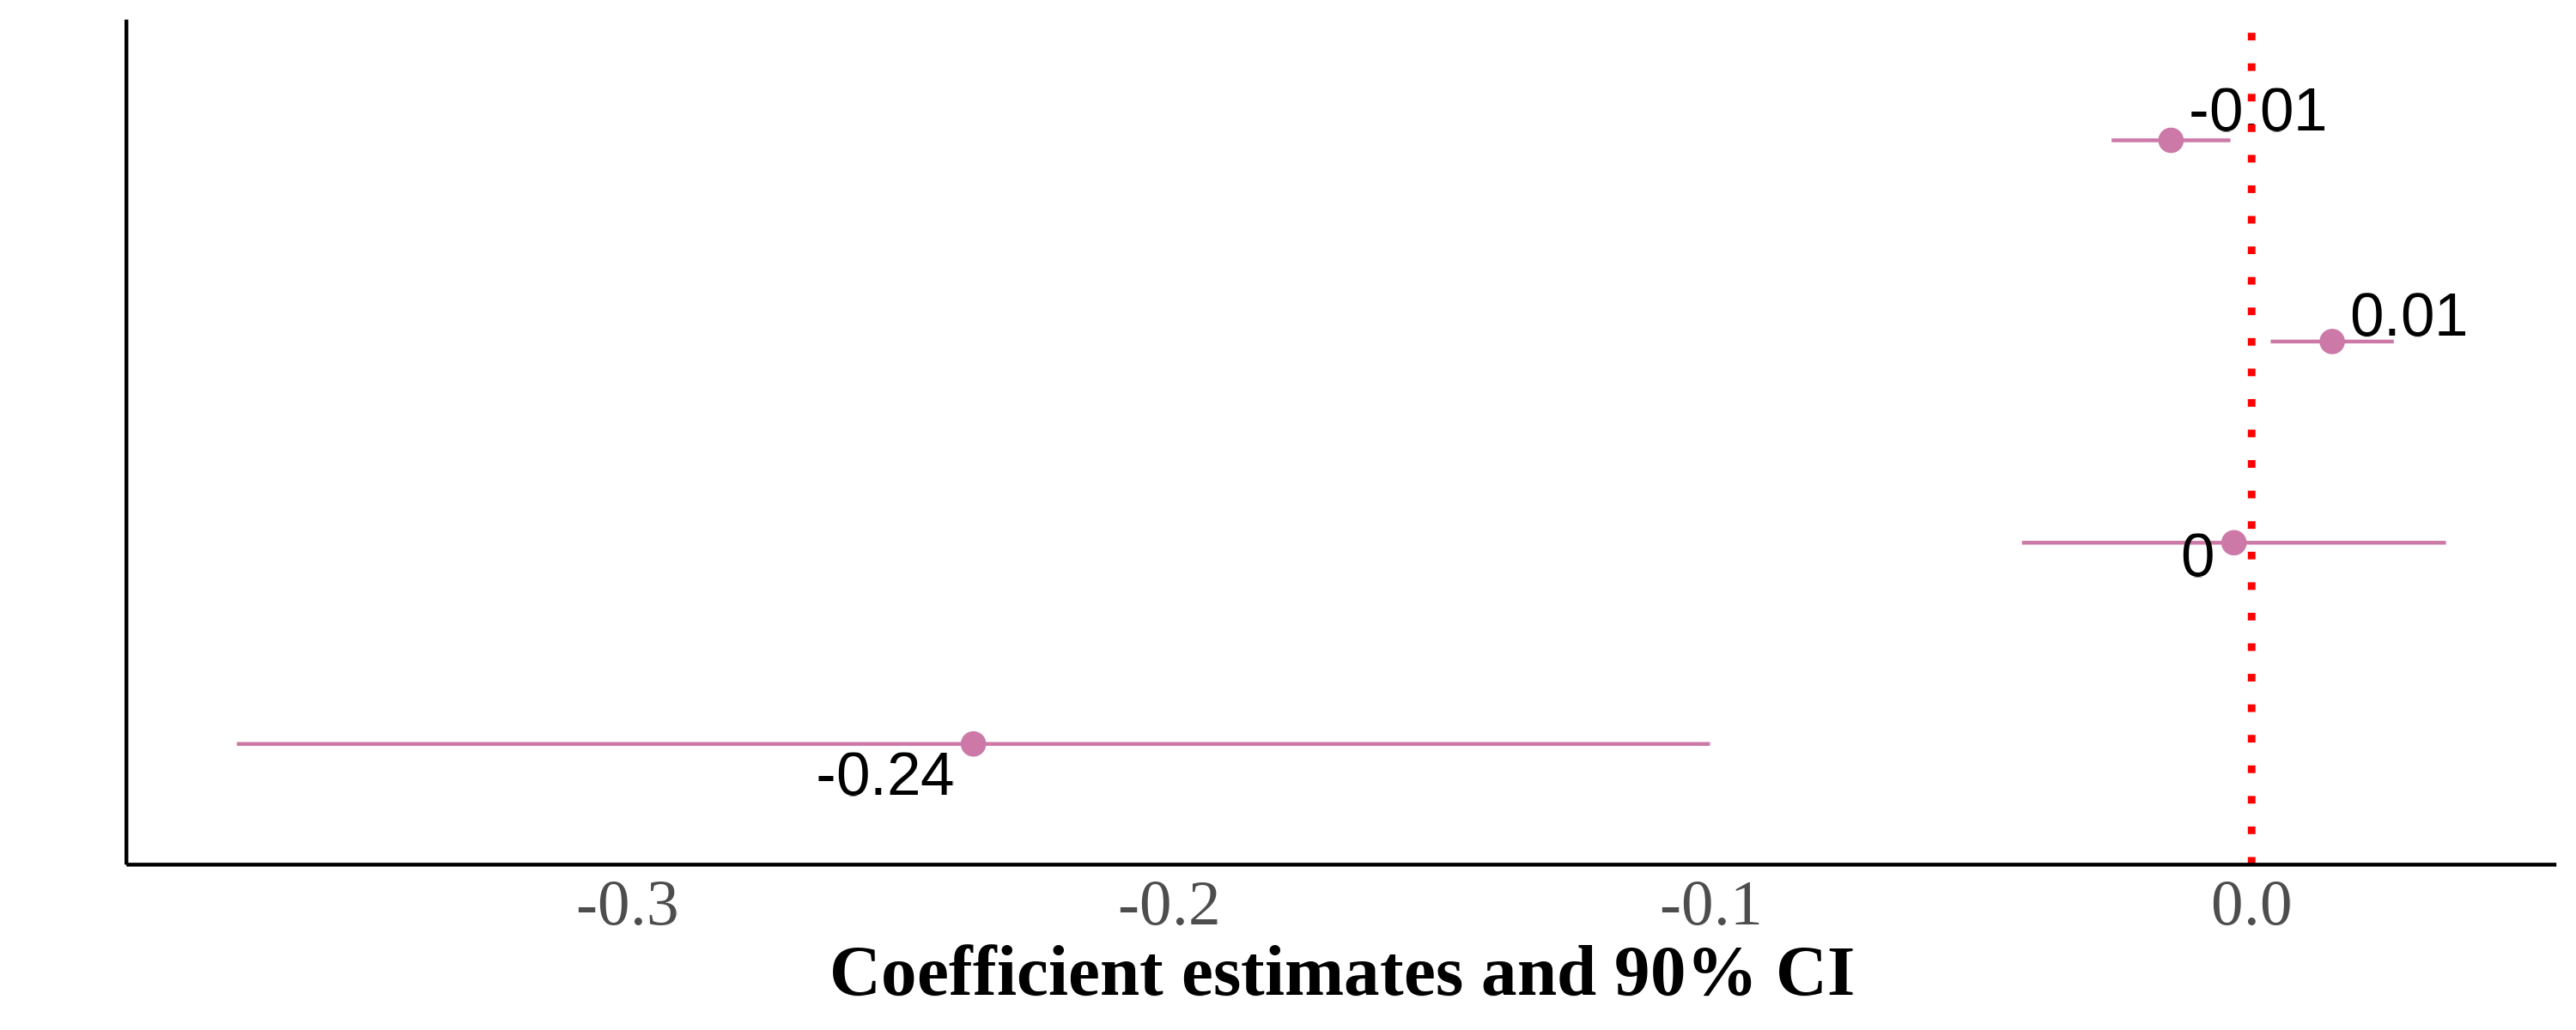
\includegraphics[width=.9\linewidth]{by-parents-regs-wh-adults.png}
\end{subfigure}
\caption*{\footnotesize{I show four panels of estimating equation (\ref{eq:identity_reg_bias}) on a sample of adults. I include region $\times$ year fixed effects with controls for sex, quartic age, years of education, and the inverse hyperbolic sine of income. The dependent variable is self-reported Asian identity and the independent variable is state-level bias. Each panel results from the same regression but on different samples divided by parental types. Standard errors are clustered on the state level. The samples include second-generation Asian individuals ages 18 and above. Native-born second-generation Asian immigrant individuals with at least one parent born in an Asian country.}}
\end{figure}
\end{center}

\pagebreak
\newpage

\begin{center}
\begin{figure}[!htb]
\centering
\caption{Multinomial Logit Model: Predicted Probabilities of Racial Identity Choice by Key Covariates (All Generations)}
\label{fig:pp-all-gen}

\begin{subfigure}{.48\textwidth}
\caption{Anti-Asian Bias}
\centering
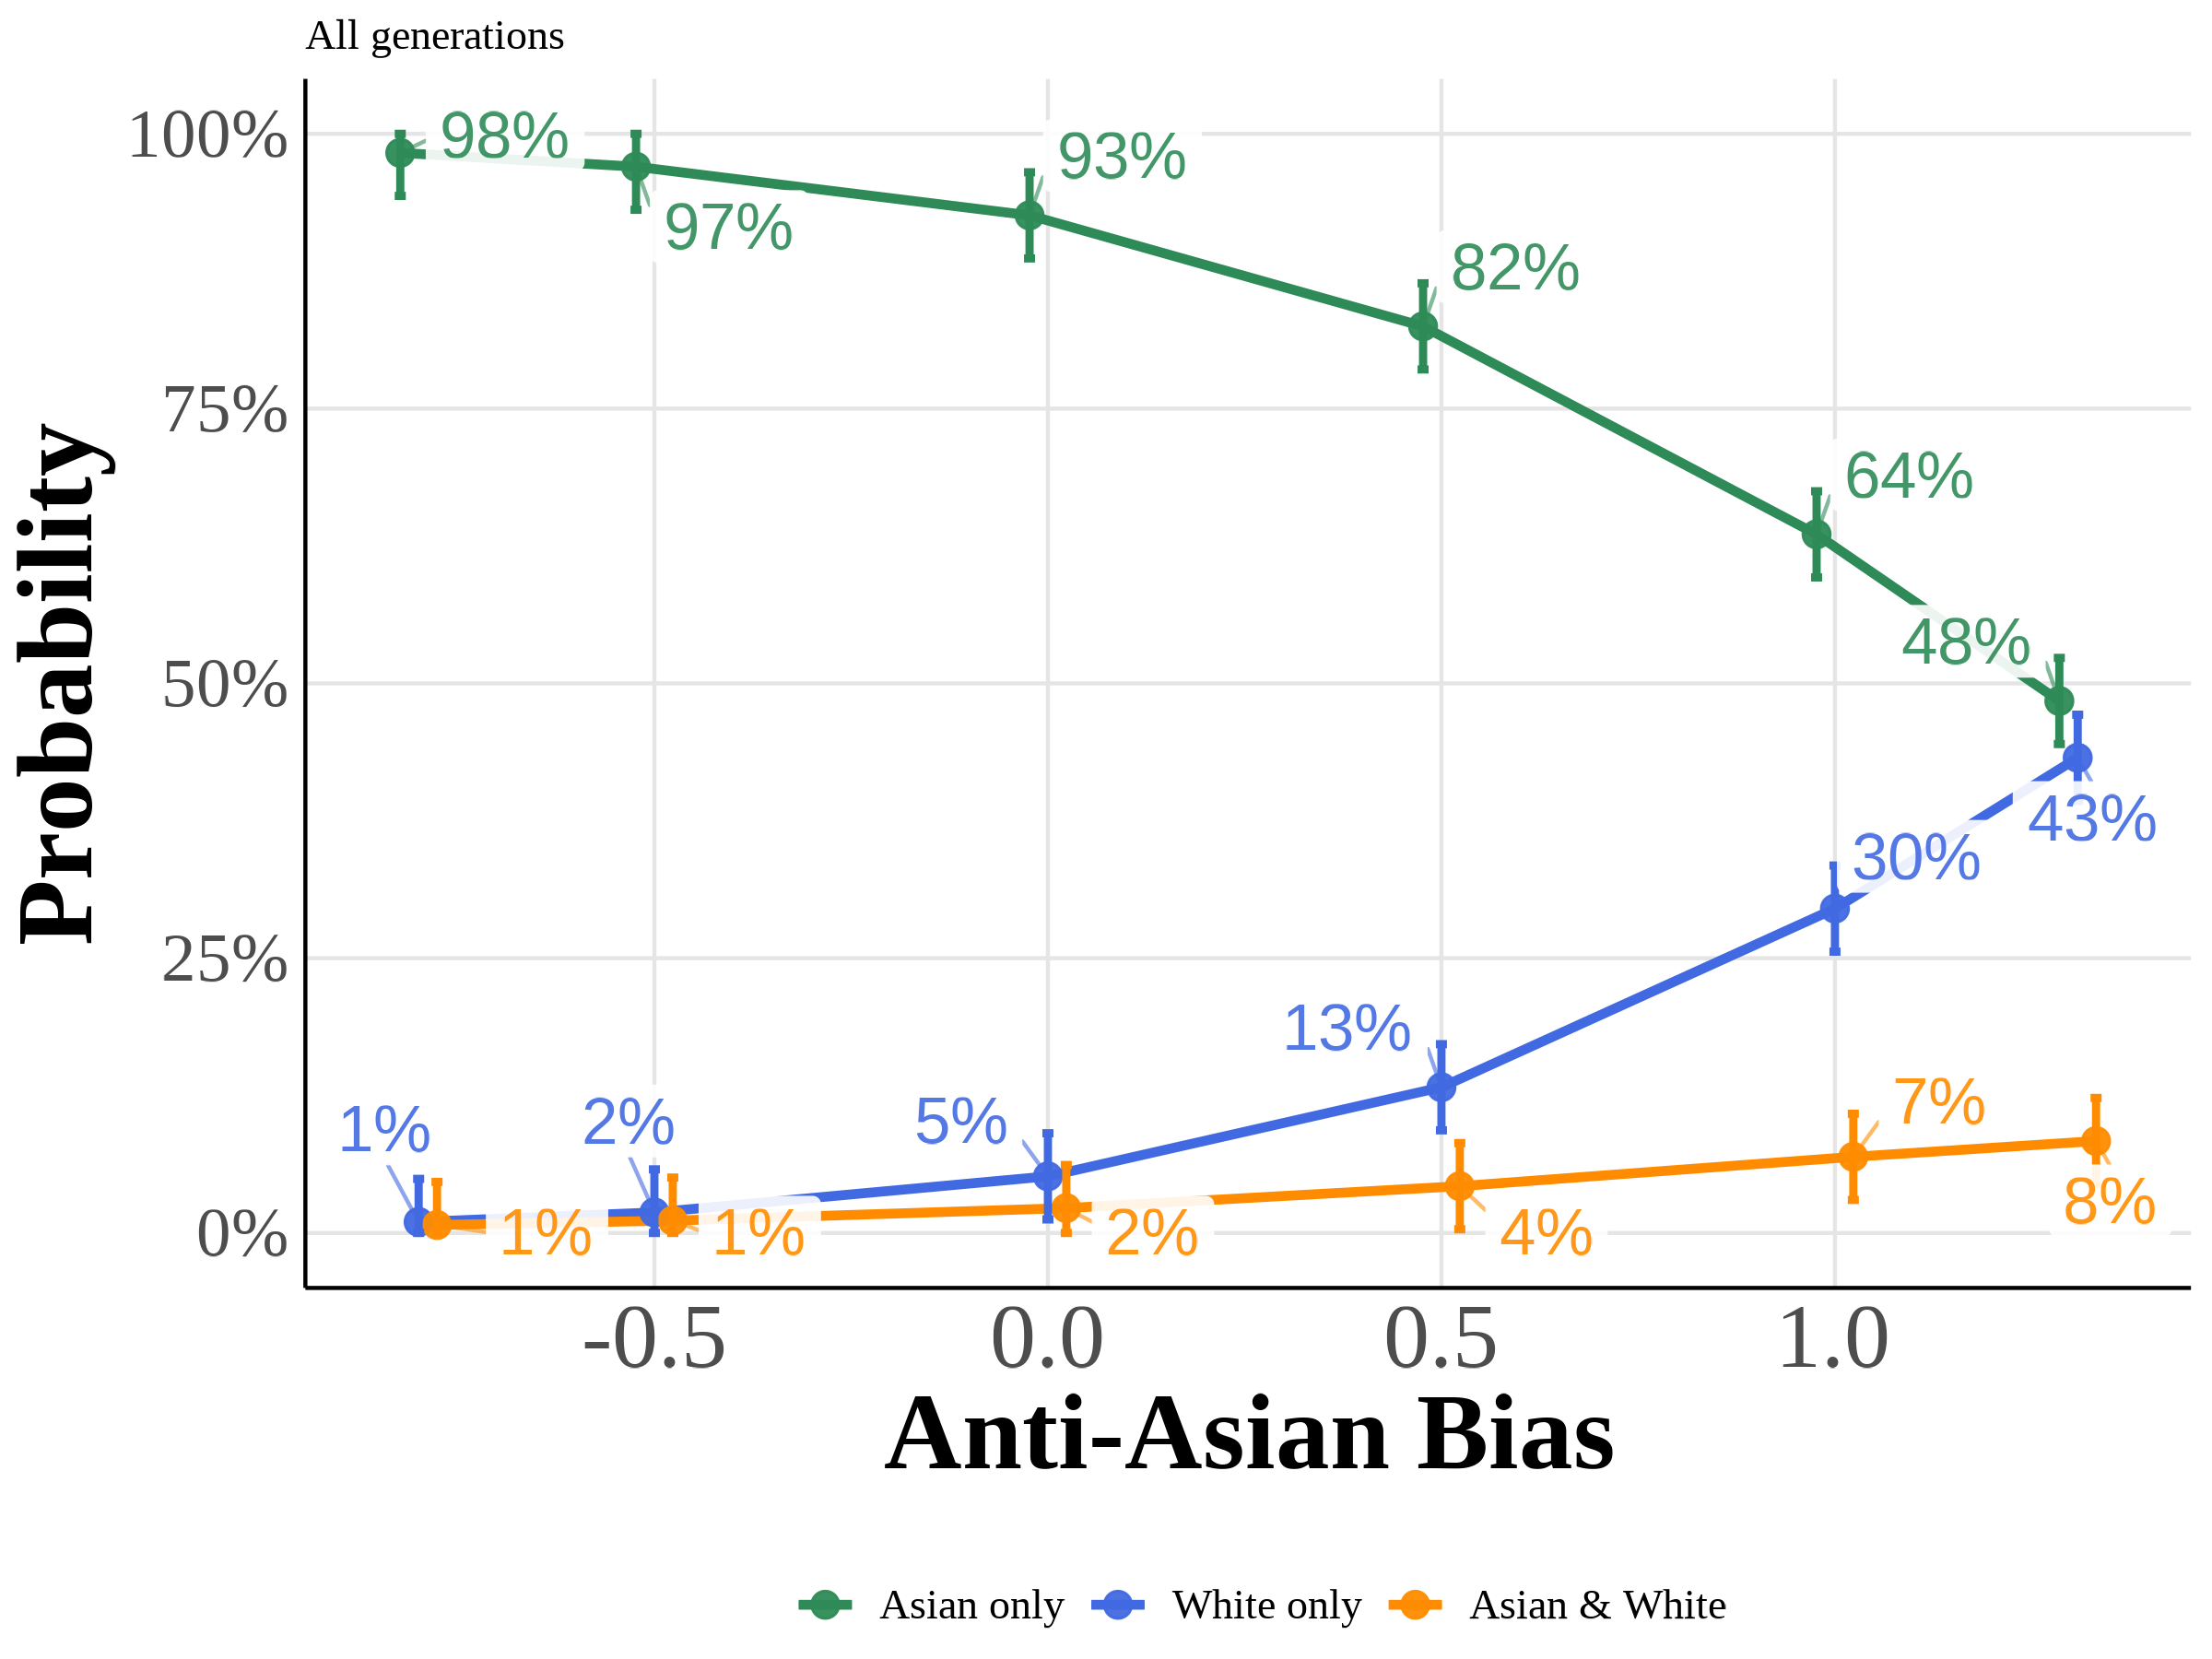
\includegraphics[width=1\linewidth]{simple_pp_value_all.png}
\end{subfigure}
\hfill
\begin{subfigure}{.48\textwidth}
\caption{Female}
\centering
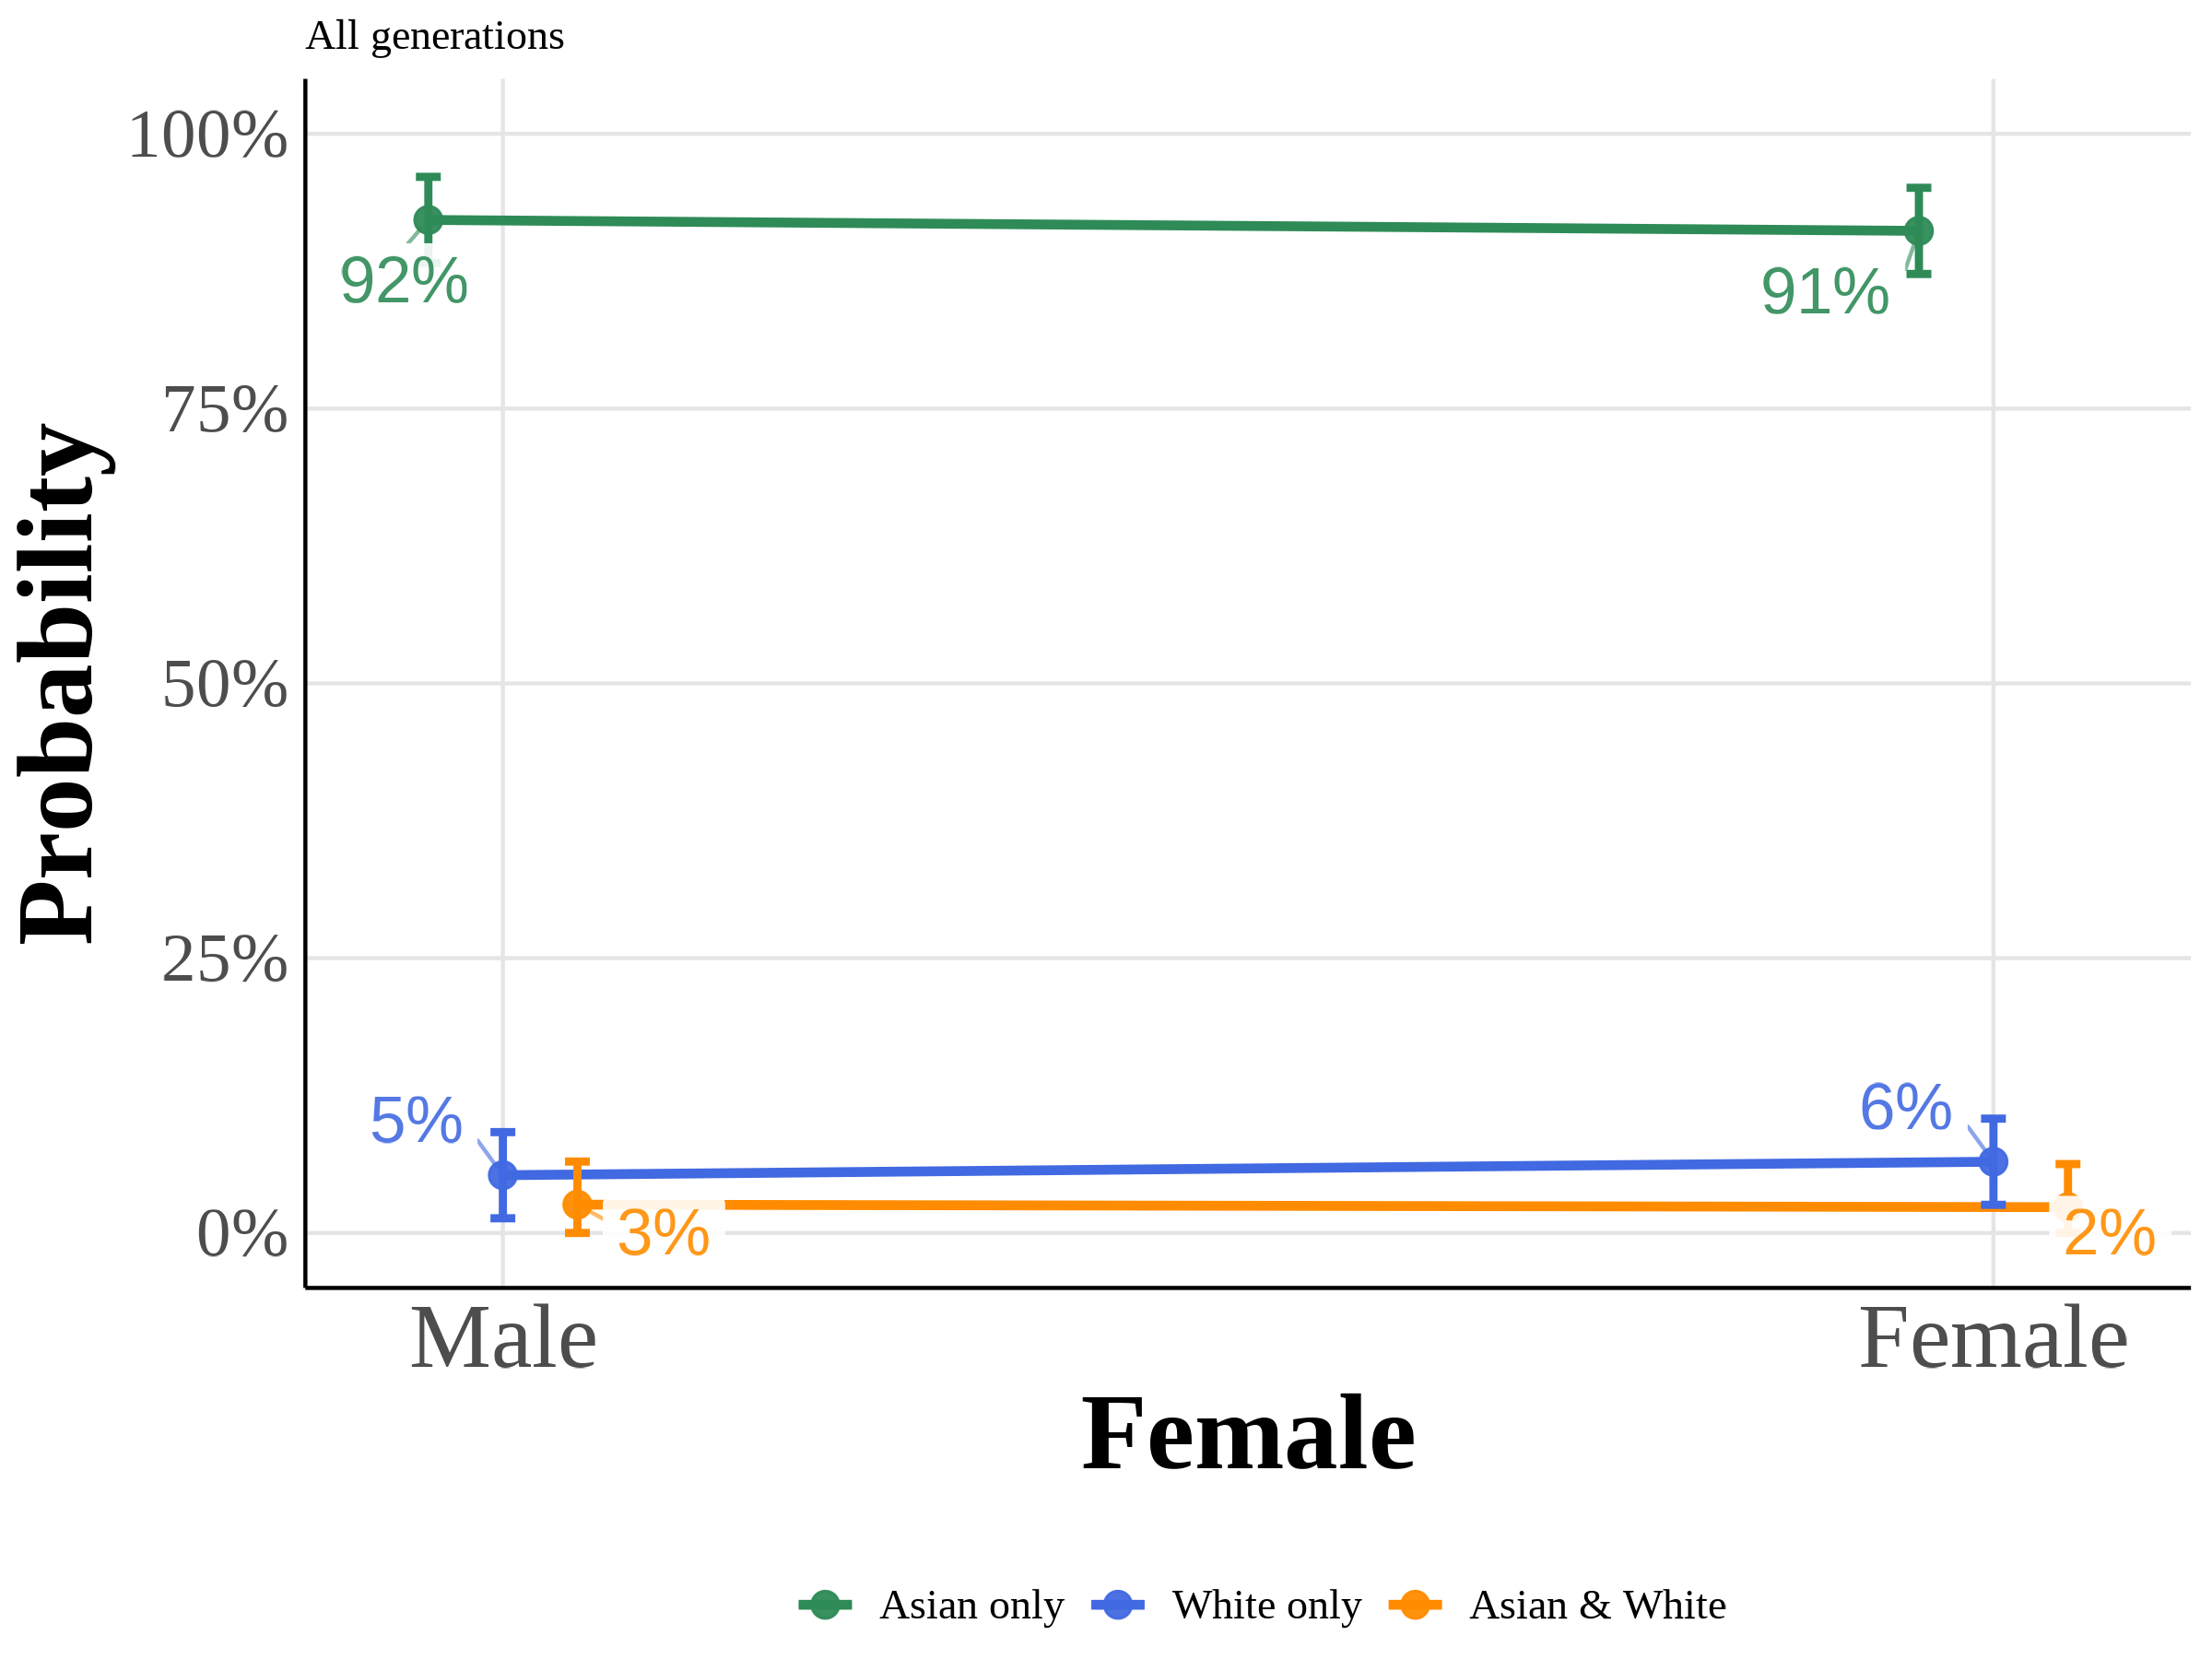
\includegraphics[width=1\linewidth]{simple_pp_Female_all.png}
\end{subfigure}

\vspace{0.5cm}

\begin{subfigure}{.48\textwidth}
\caption{College Graduate: Mother}
\centering
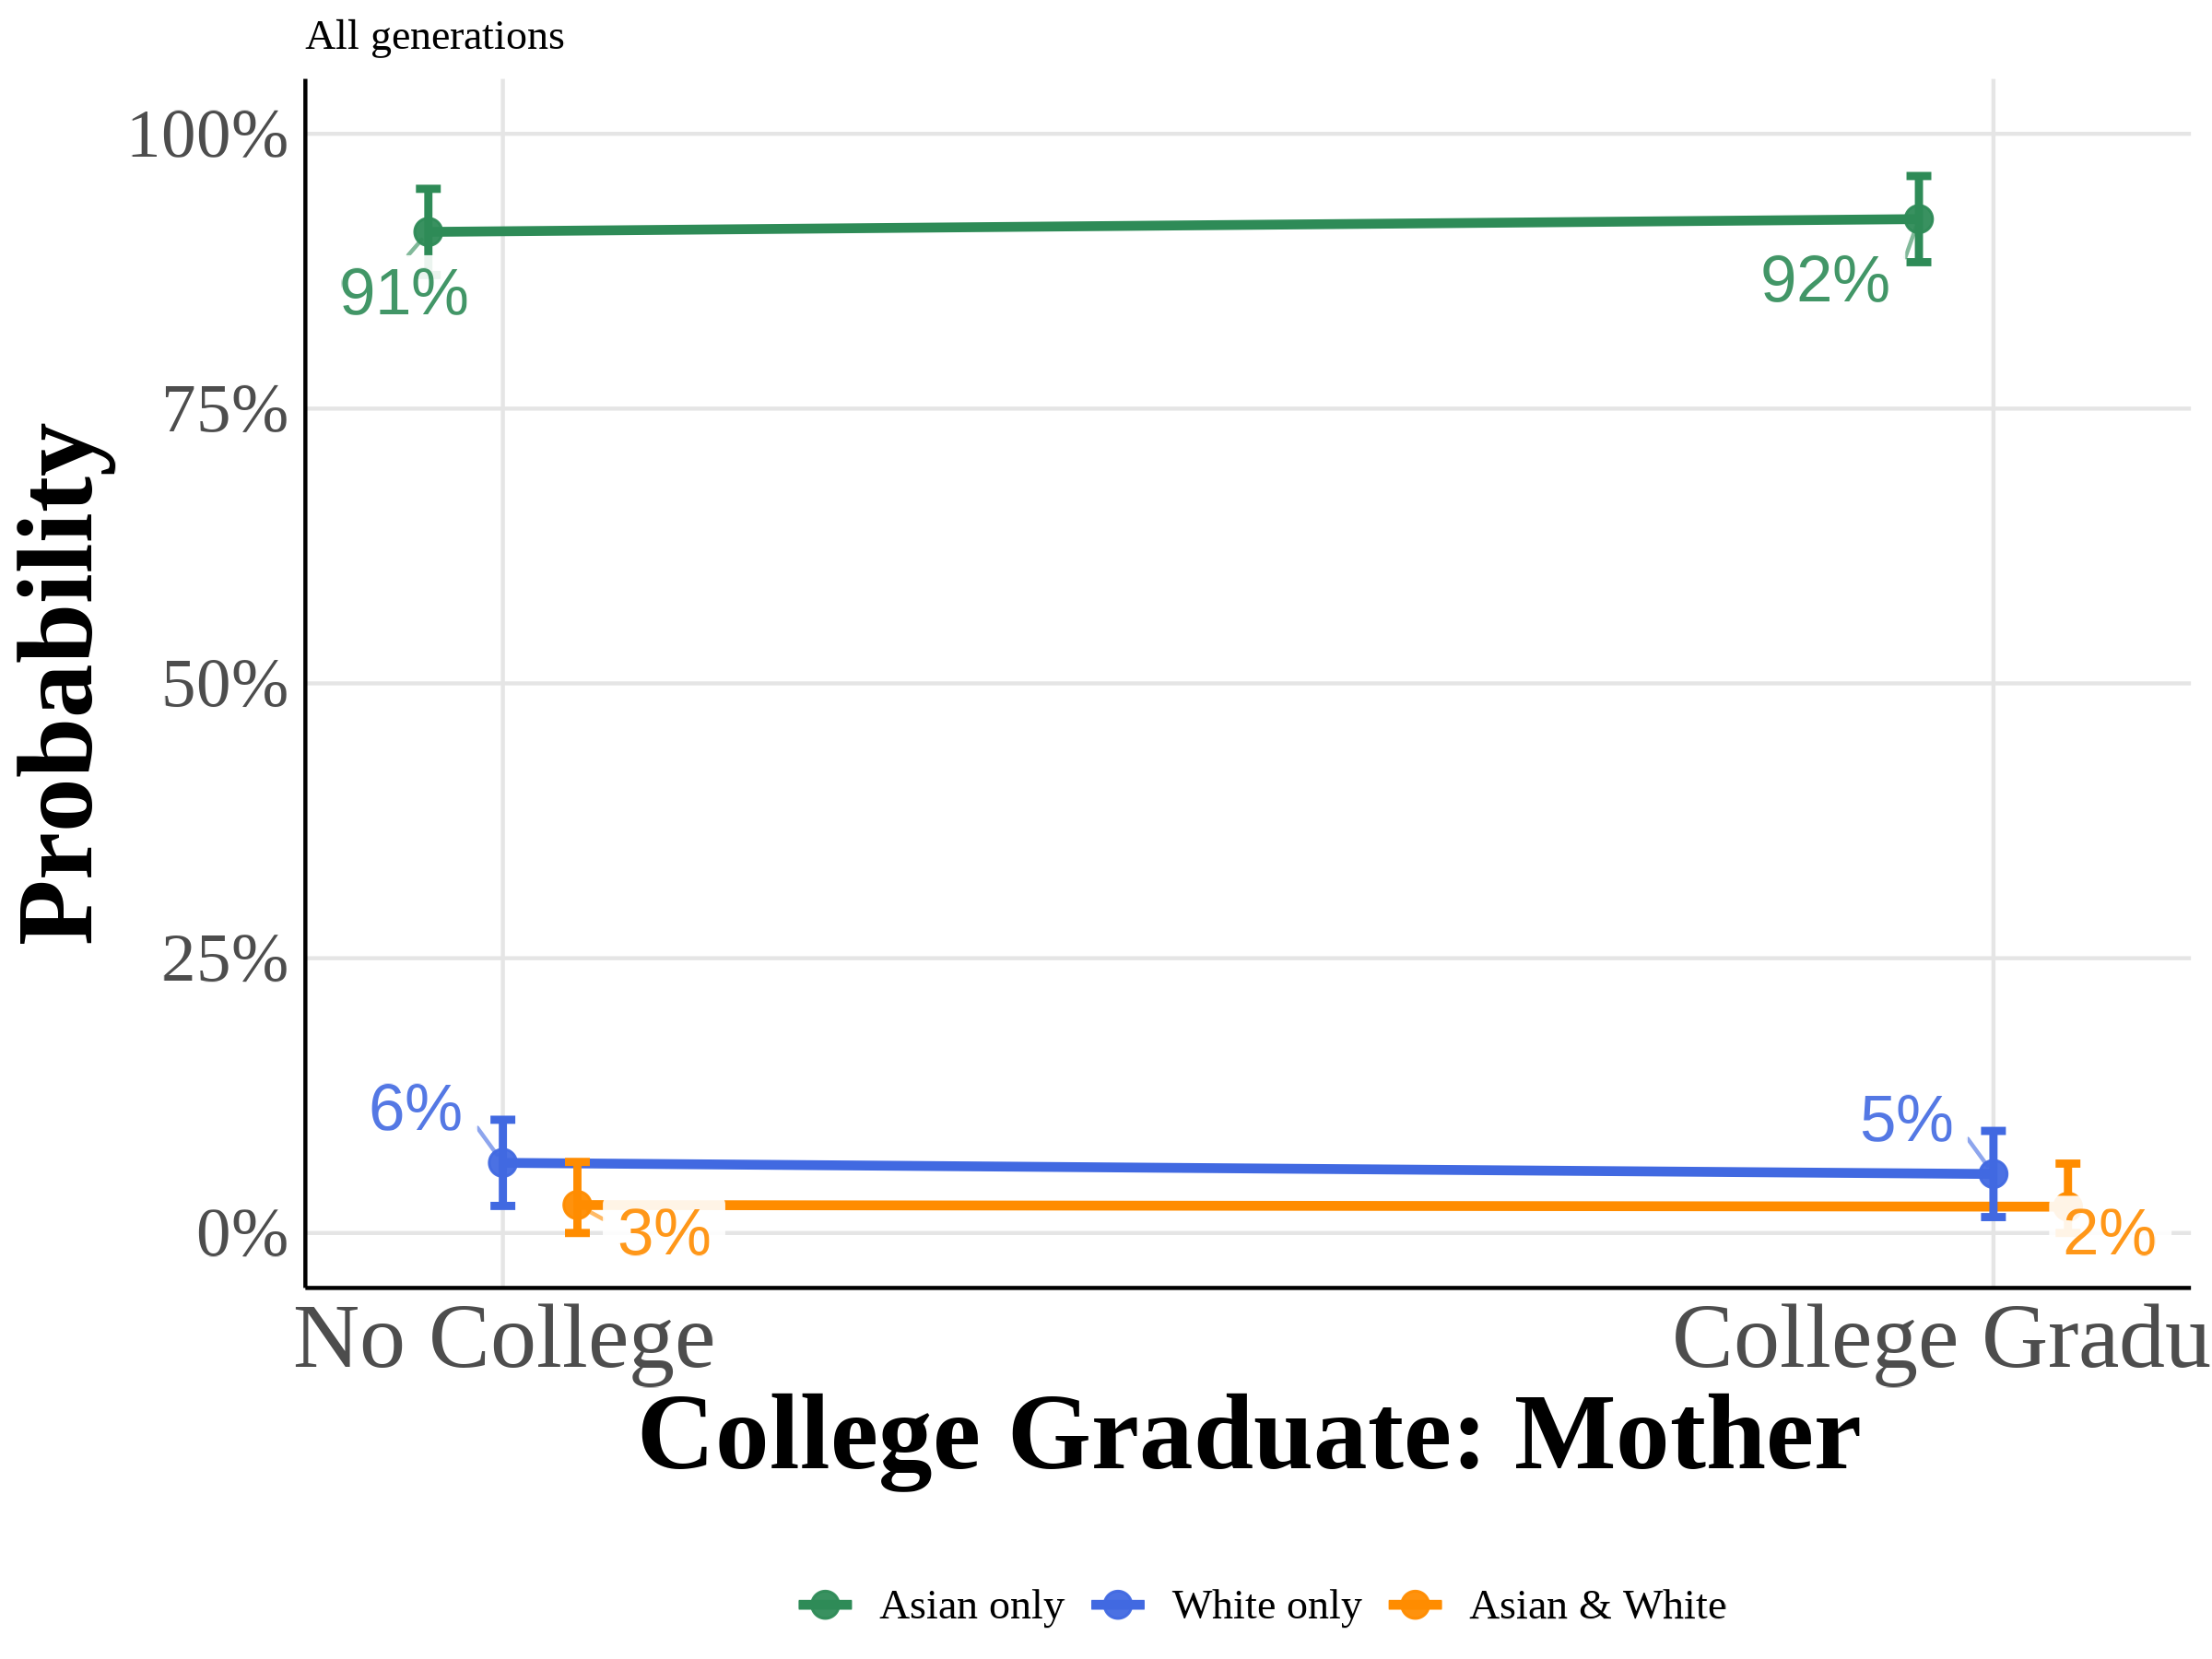
\includegraphics[width=1\linewidth]{simple_pp_MomGradCollege_all.png}
\end{subfigure}
\hfill
\begin{subfigure}{.48\textwidth}
\caption{College Graduate: Father}
\centering
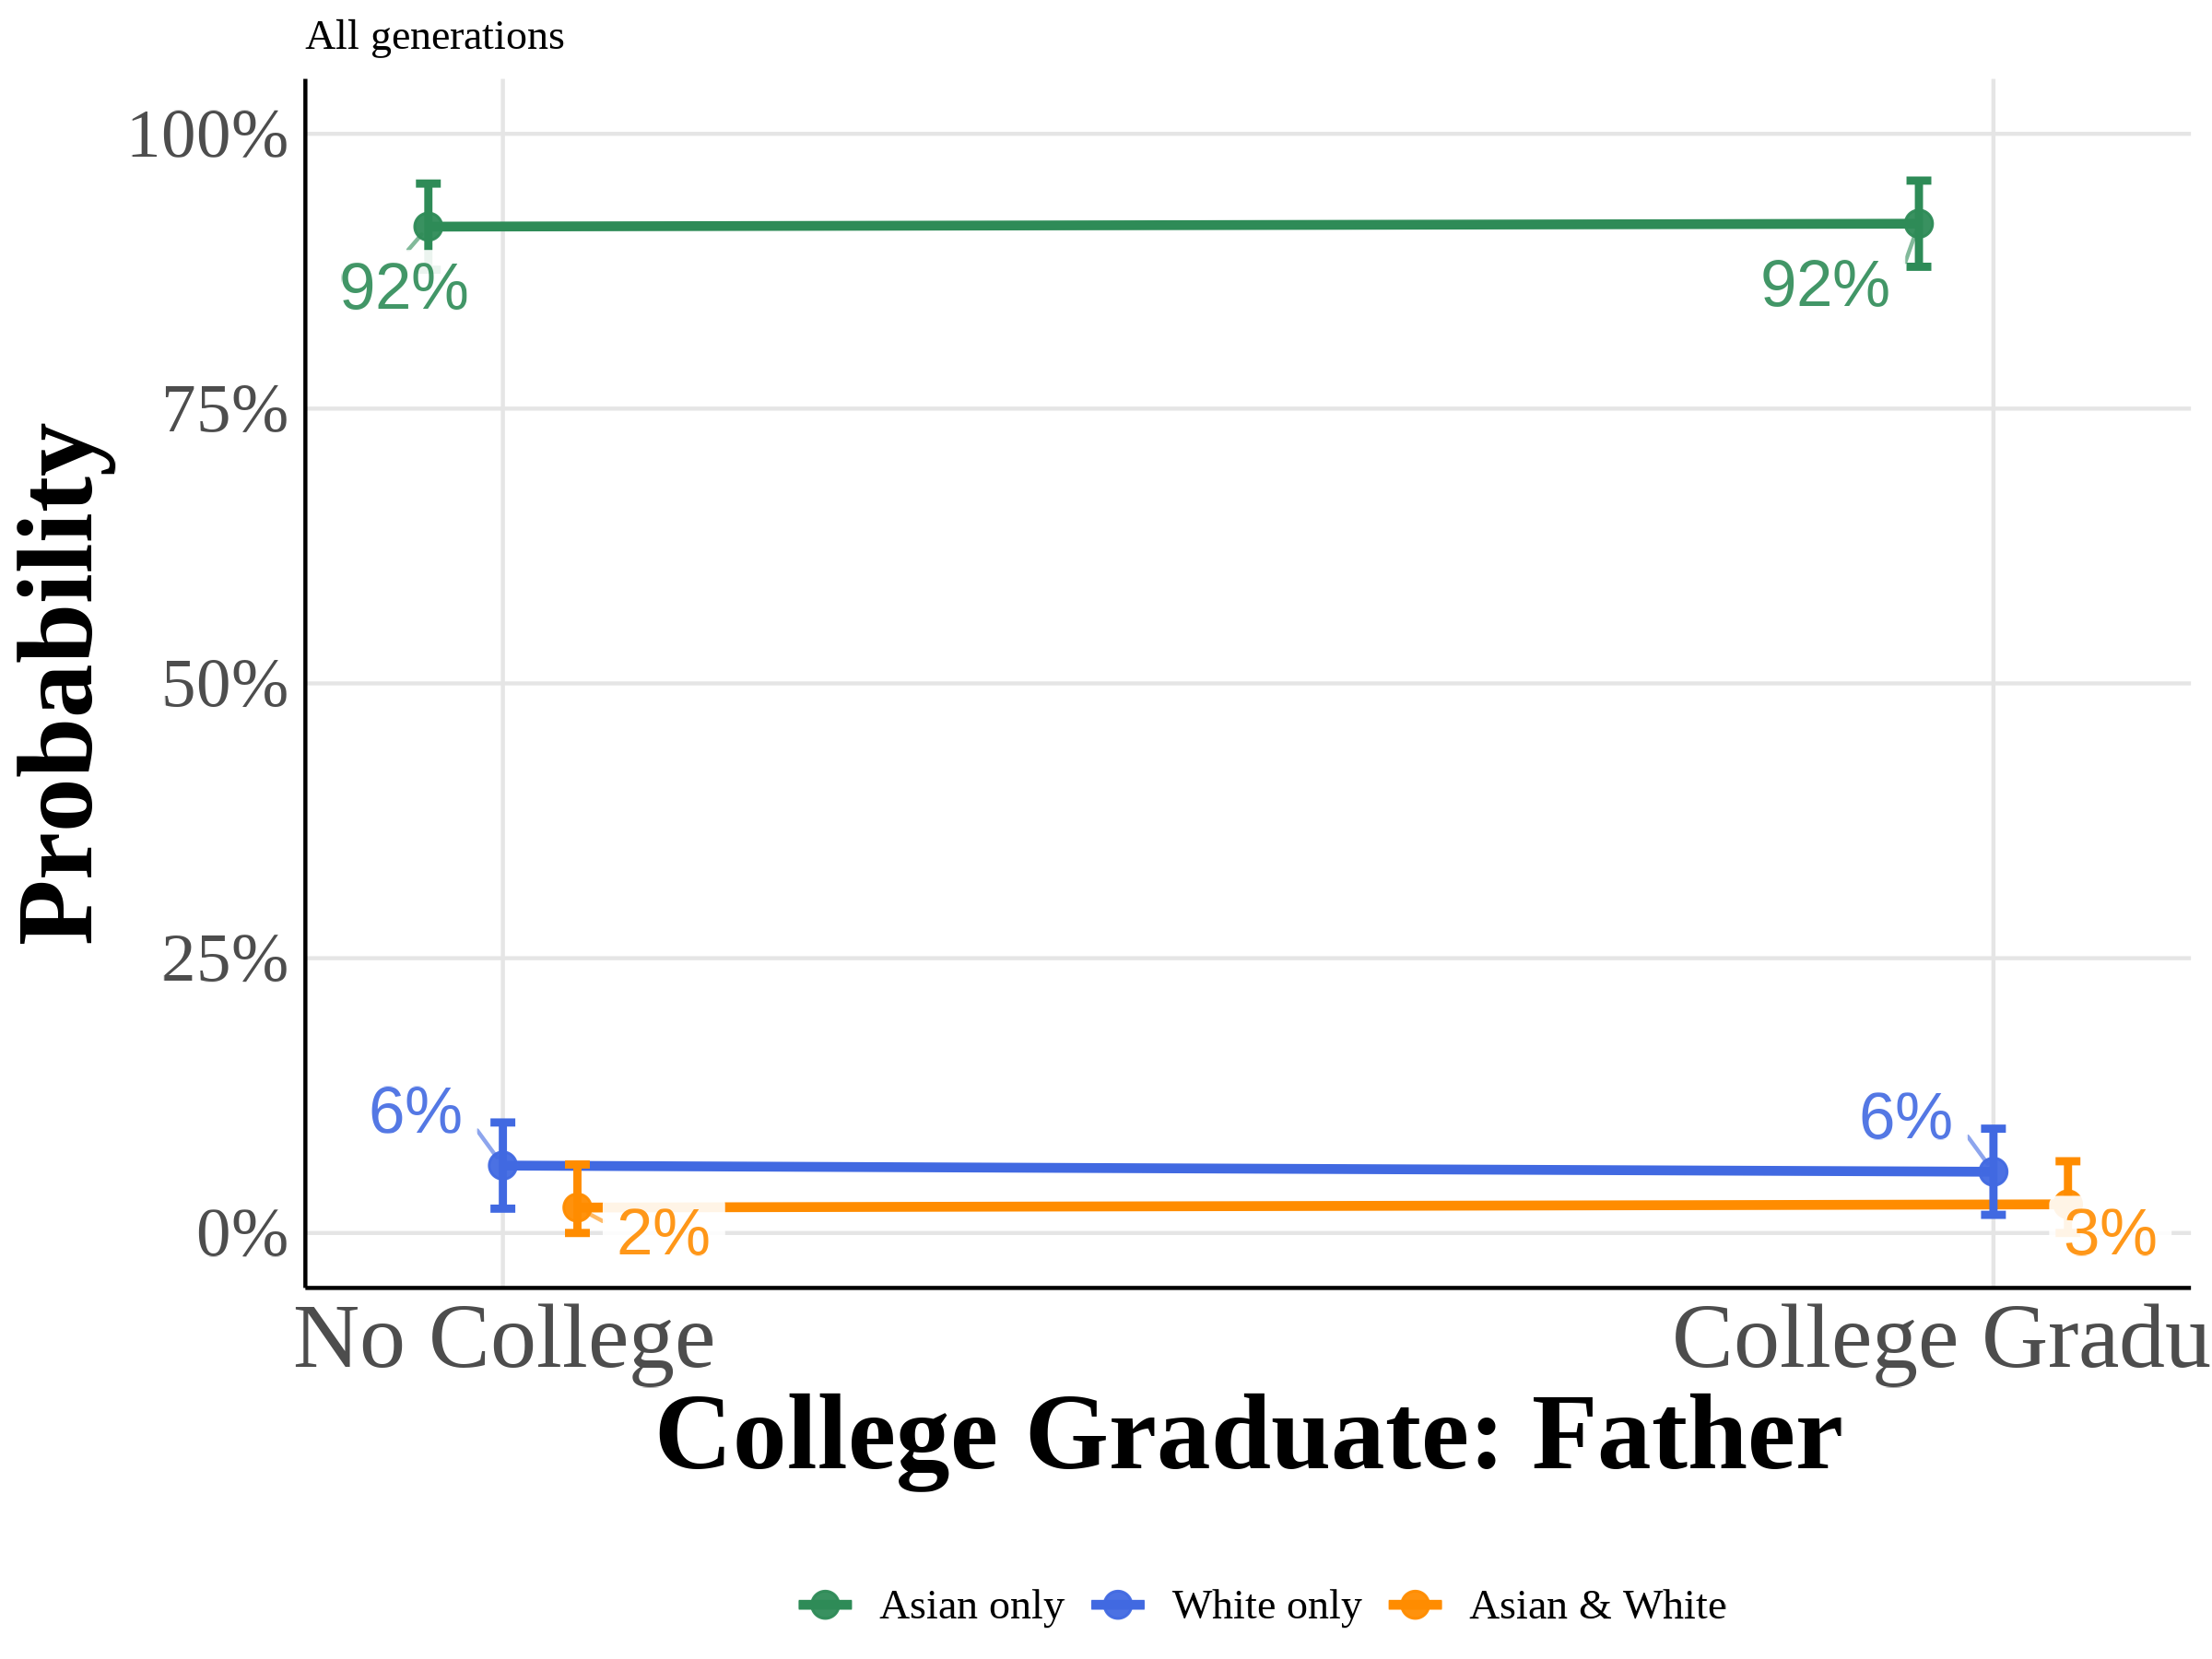
\includegraphics[width=1\linewidth]{simple_pp_DadGradCollege_all.png}
\end{subfigure}

\caption*{\footnotesize{This figure shows predicted probabilities from estimating equation (\ref{eq:multinomial_logit}) using a multinomial logit model. The model estimates the probability of choosing ``Asian only'', ``White only'', or ``Asian and White'' racial identification as a function of anti-Asian bias, gender, and parental education. I include region $\times$ year fixed effects with controls for quartic age and local Asian population share. All other variables are held at their sample means. The analysis includes first-, second-, and third-generation Asian Americans. First-generation Asian Americans are foreign-born individuals. Second-generation Asian Americans are native-born individuals with at least one Asian-born parent. Third-generation Asian Americans are native-born individuals with native-born parents and at least one Asian-born grandparent.}}
\end{figure}
\end{center}

% \pagebreak
% \newpage

% % Marginal Effects: All Generations (after main Multinomial Logit Model plot)
% \begin{center}
% \begin{figure}[!htb]
% \centering
% \caption{Marginal Effects of Key Covariates on Racial Identity Choice from Multinomial Logit Model (All Generations)}
% \label{fig:marginal-effects-all}
% 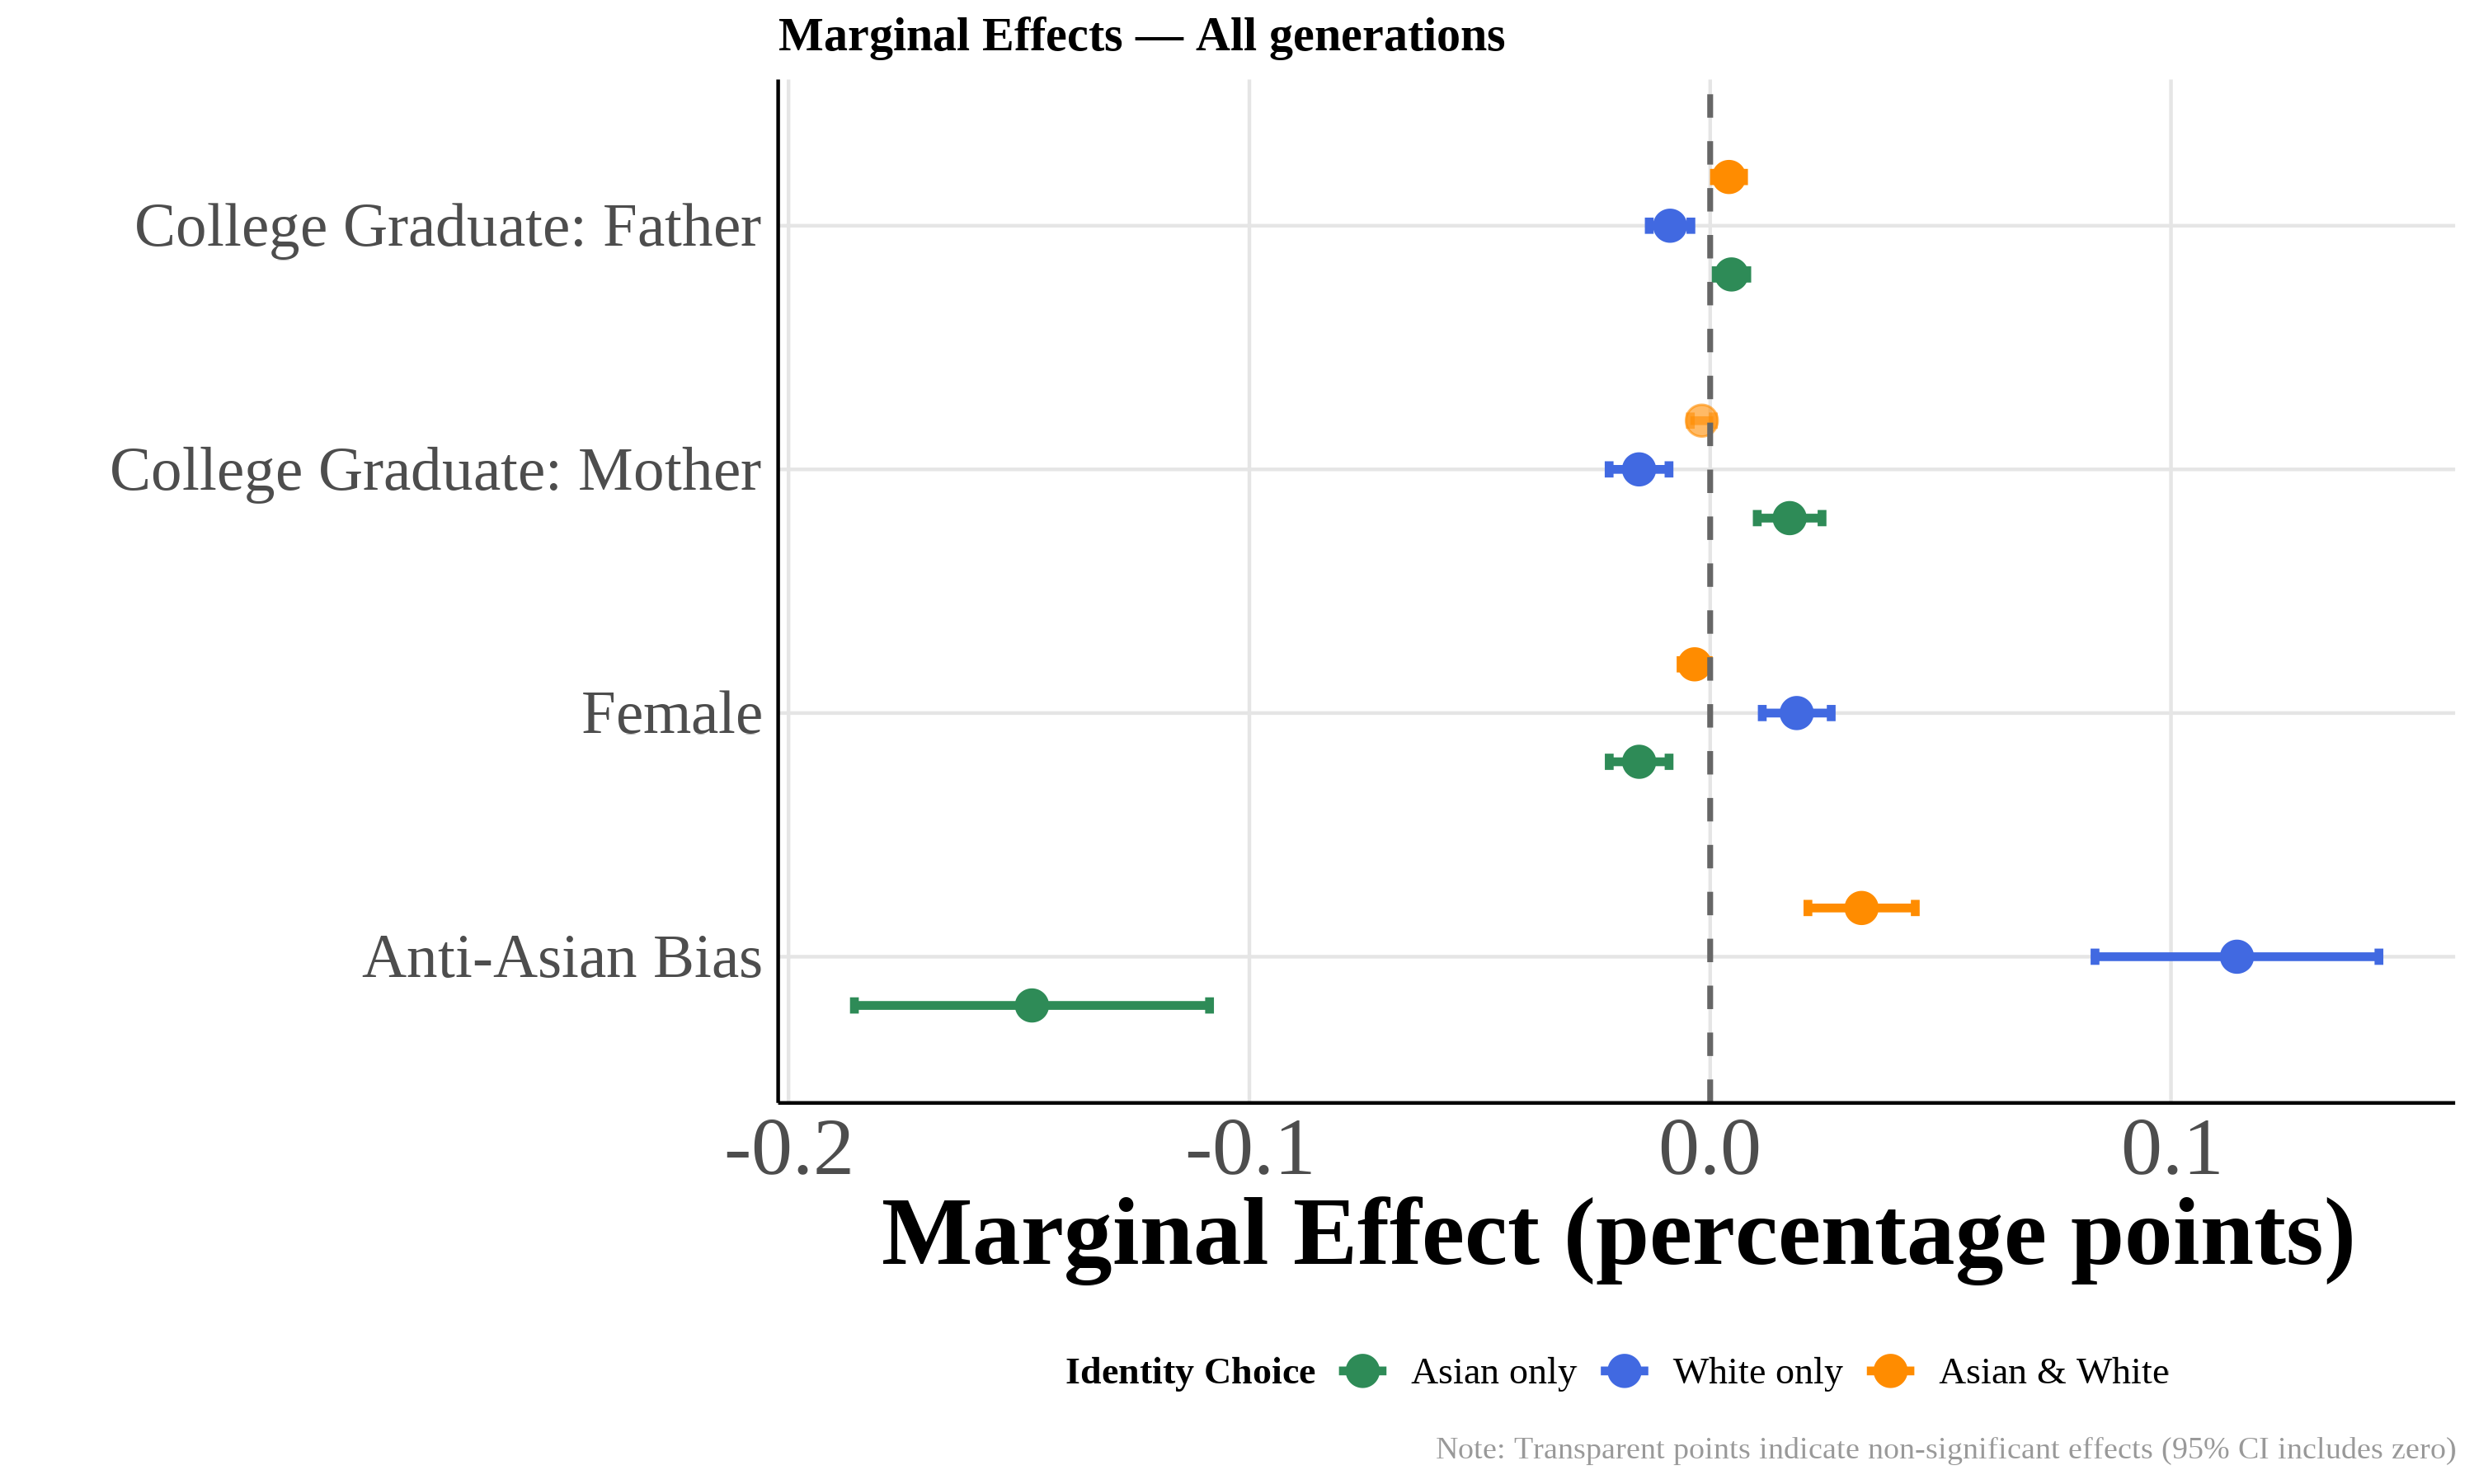
\includegraphics[width=0.9\linewidth]{optimized_marginal_effects_all.png}
% \caption*{\footnotesize{This figure displays the marginal effects of key covariates on the probability of each racial identification outcome, estimated from equation (\ref{eq:multinomial_logit}) using a multinomial logit model. Marginal effects represent the change in predicted probability for a one-unit increase in the covariate (or discrete change from 0 to 1 for binary variables), holding other variables at their sample means. I include region $\times$ year fixed effects with controls for quartic age and local Asian population share. Error bars indicate 95\% confidence intervals. The sample includes first-, second-, and third-generation Asian Americans as defined above.}}
% \end{figure}
% \end{center}

\pagebreak
\newpage


\begin{center}
\begin{figure}[!htb]
\centering
\caption{Multinomial Logit Model: Predicted Probabilities of Racial Identity Choice by Key Covariates (Second-Generation Asian Americans with Asian Fathers and White Mothers)}
\label{fig:pp-second-aw}

\begin{subfigure}{.48\textwidth}
\caption{Anti-Asian Bias}
\centering
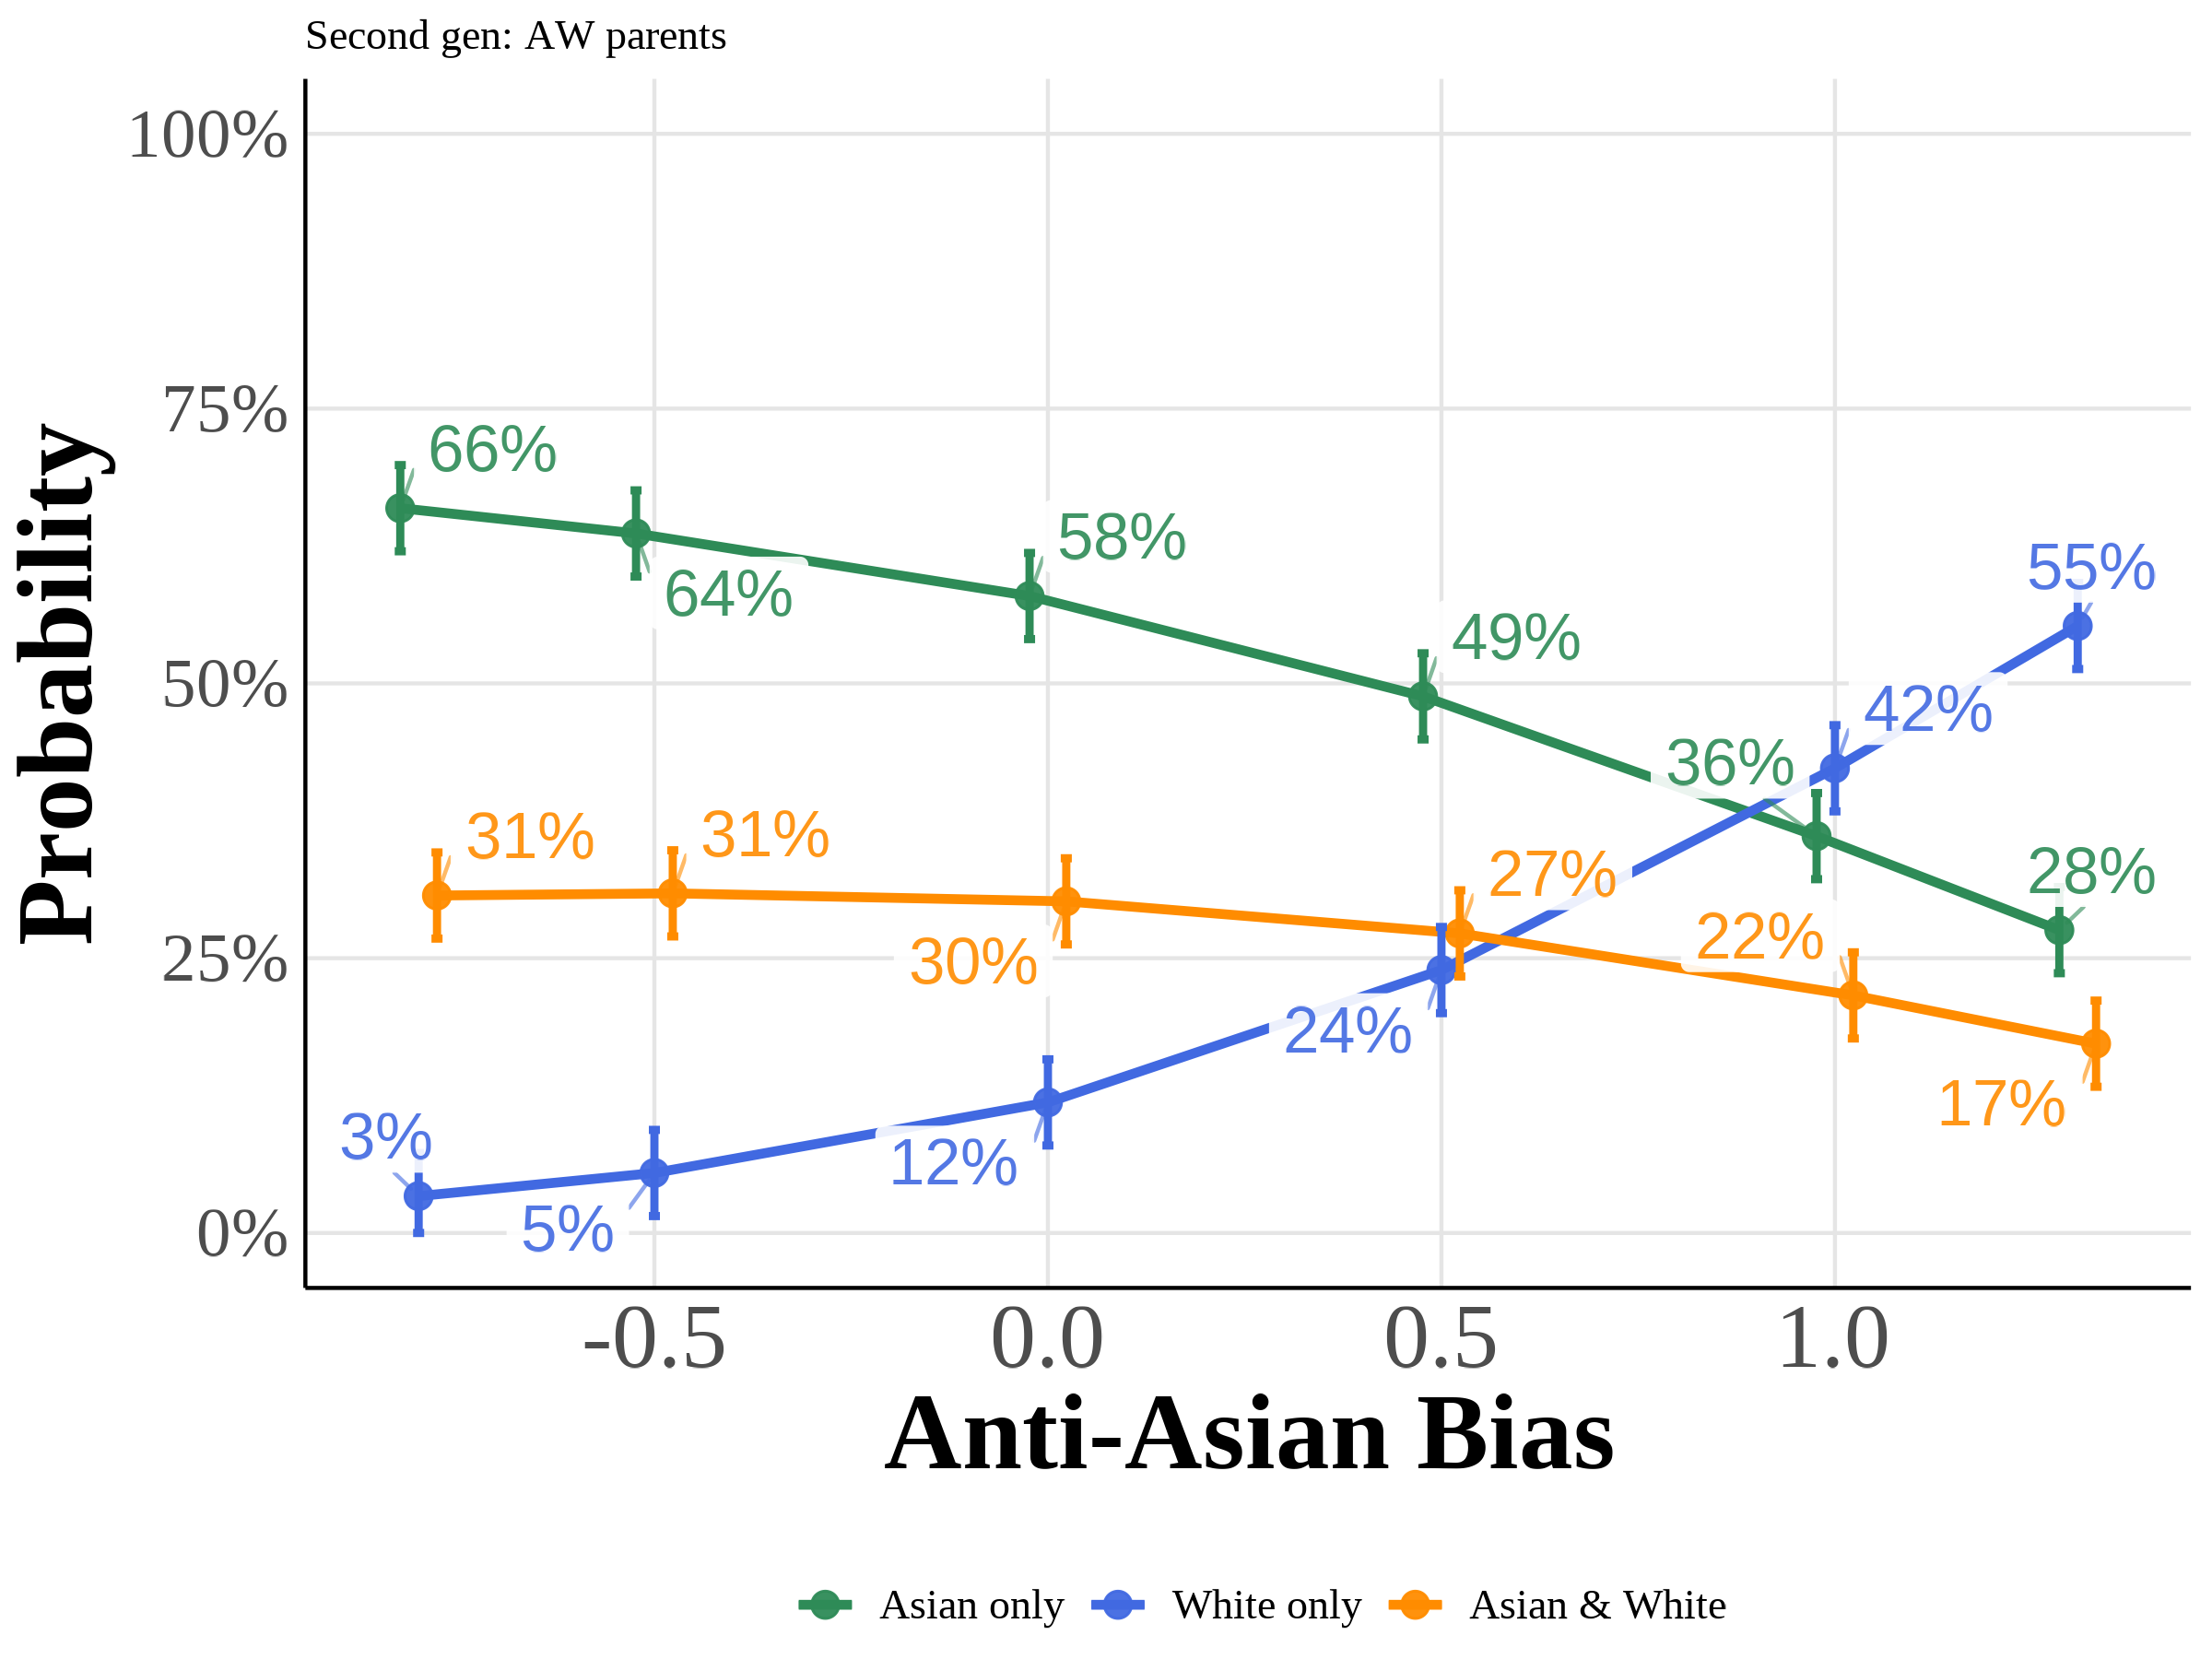
\includegraphics[width=1\linewidth]{simple_pp_value_second_aw.png}
\end{subfigure}
\hfill
\begin{subfigure}{.48\textwidth}
\caption{Female}
\centering
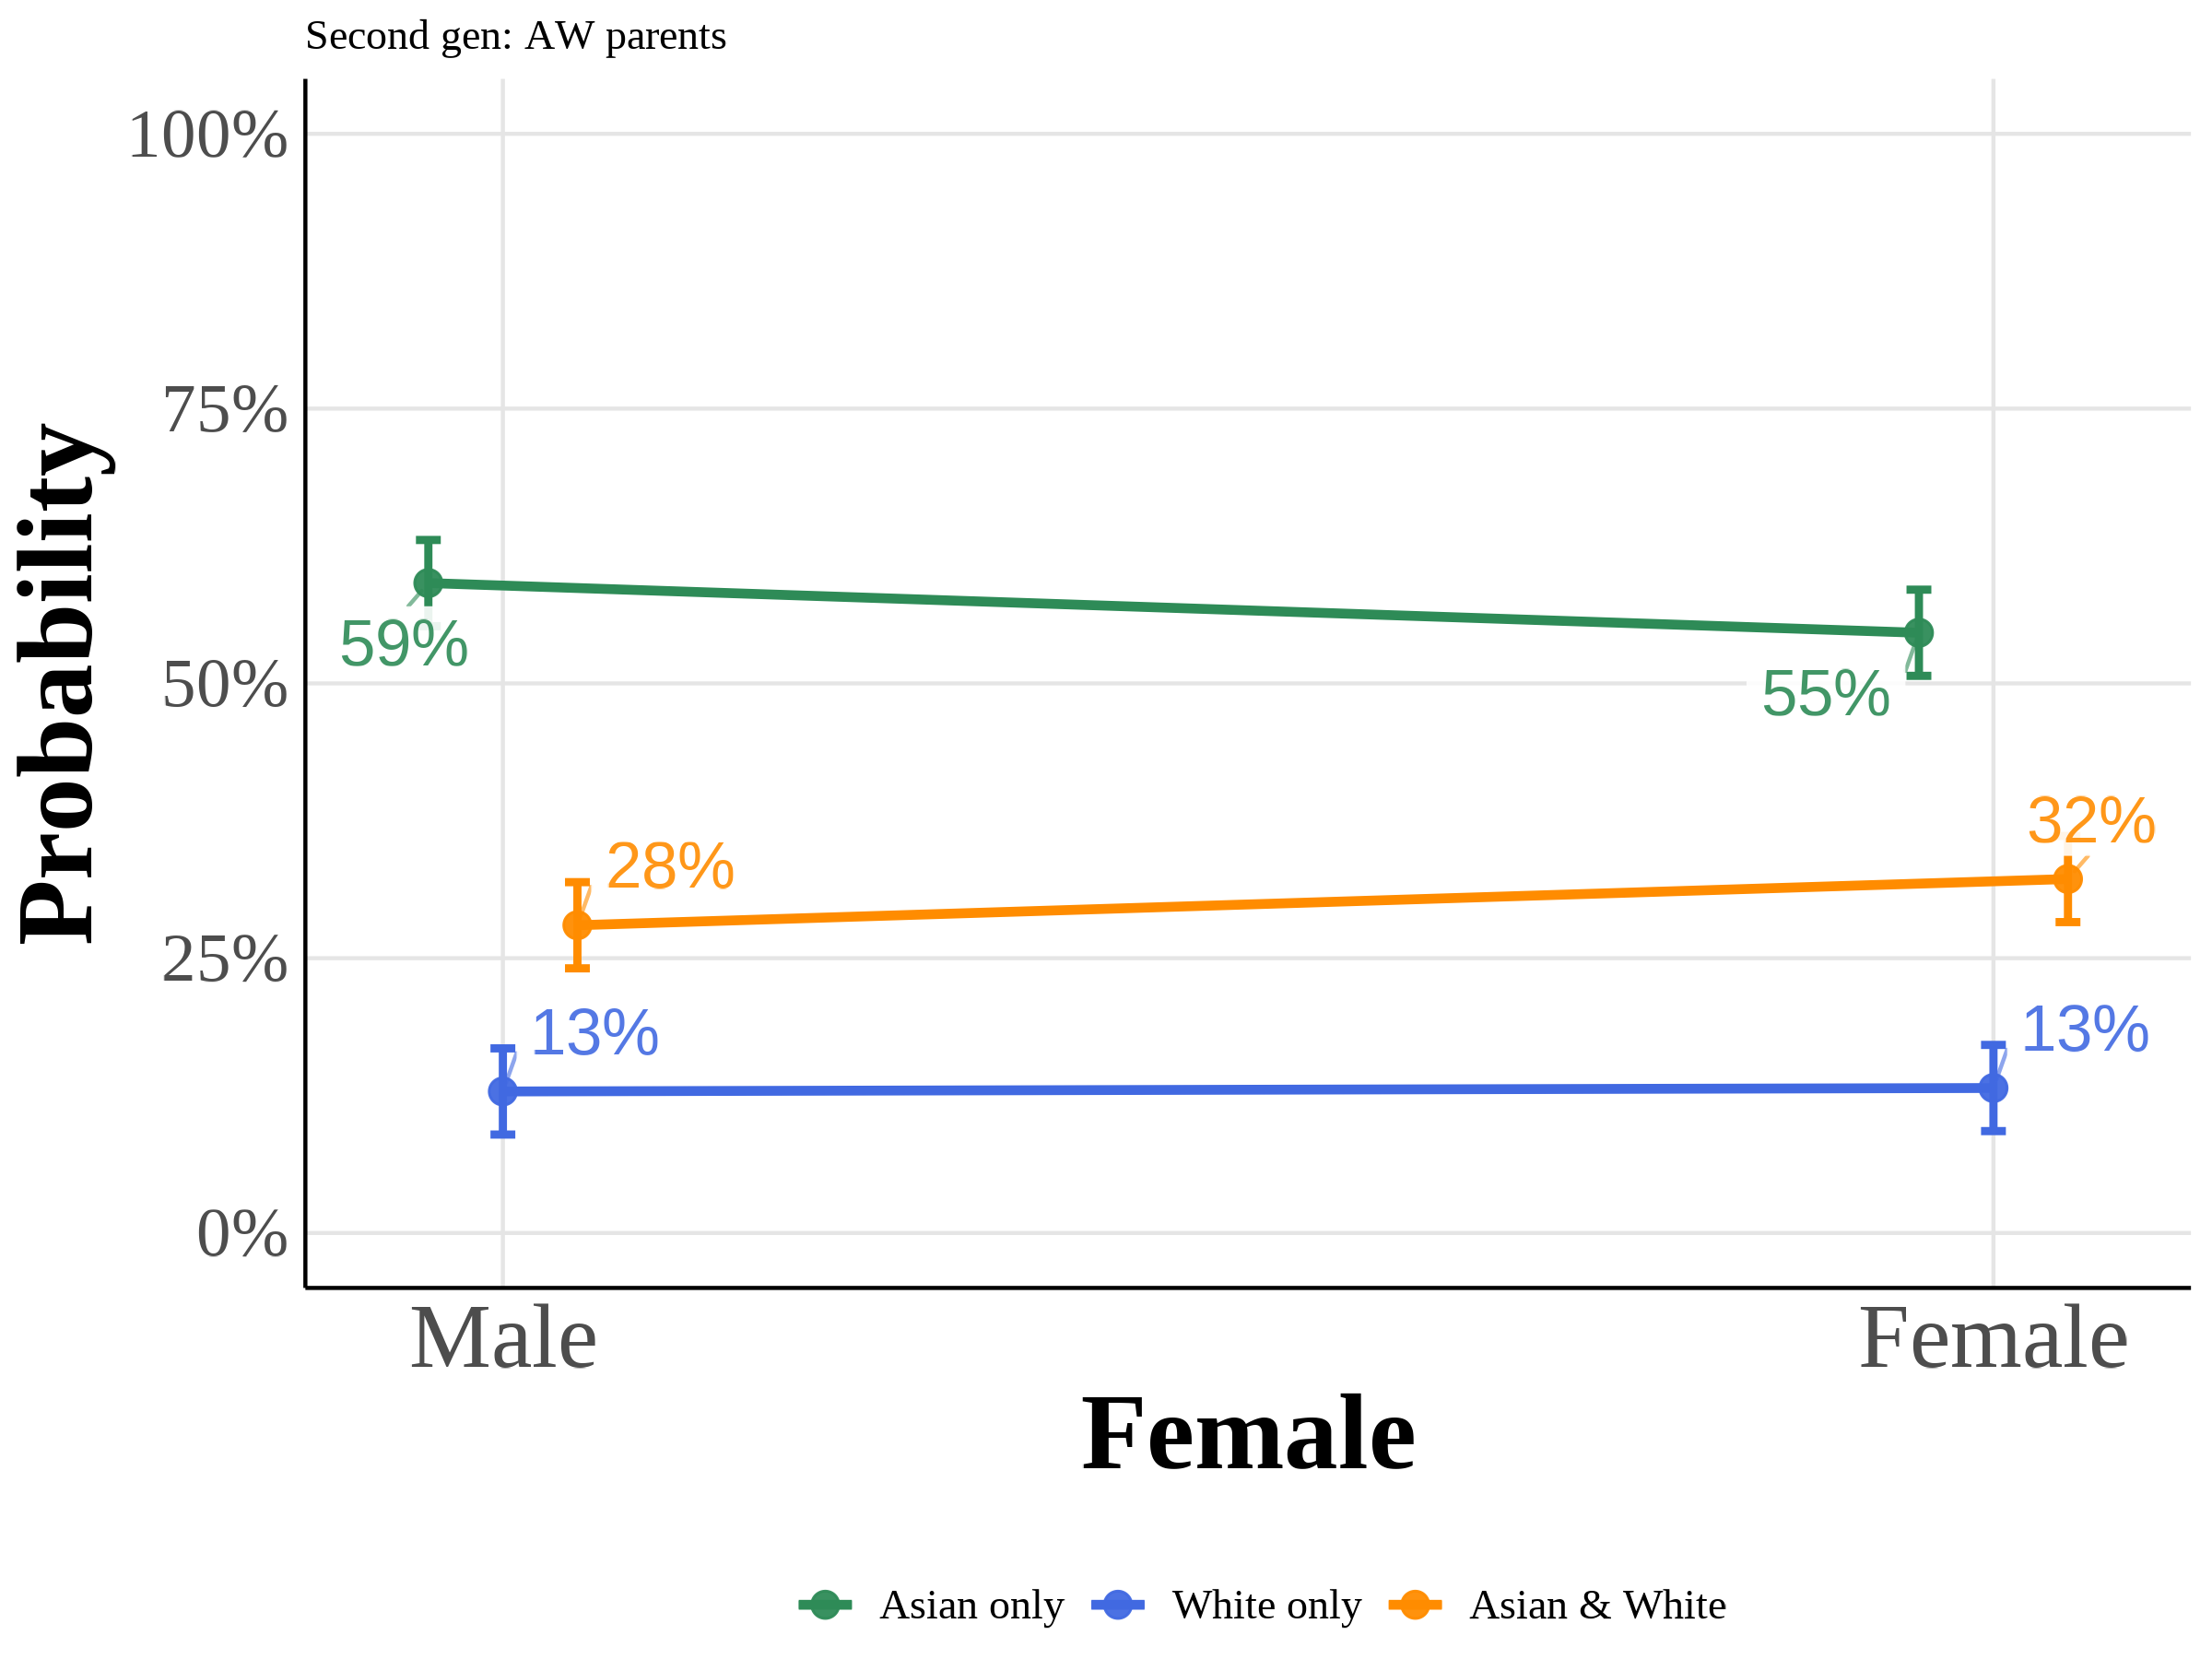
\includegraphics[width=1\linewidth]{simple_pp_Female_second_aw.png}
\end{subfigure}

\vspace{0.5cm}

\begin{subfigure}{.48\textwidth}
\caption{College Graduate: Mother}
\centering
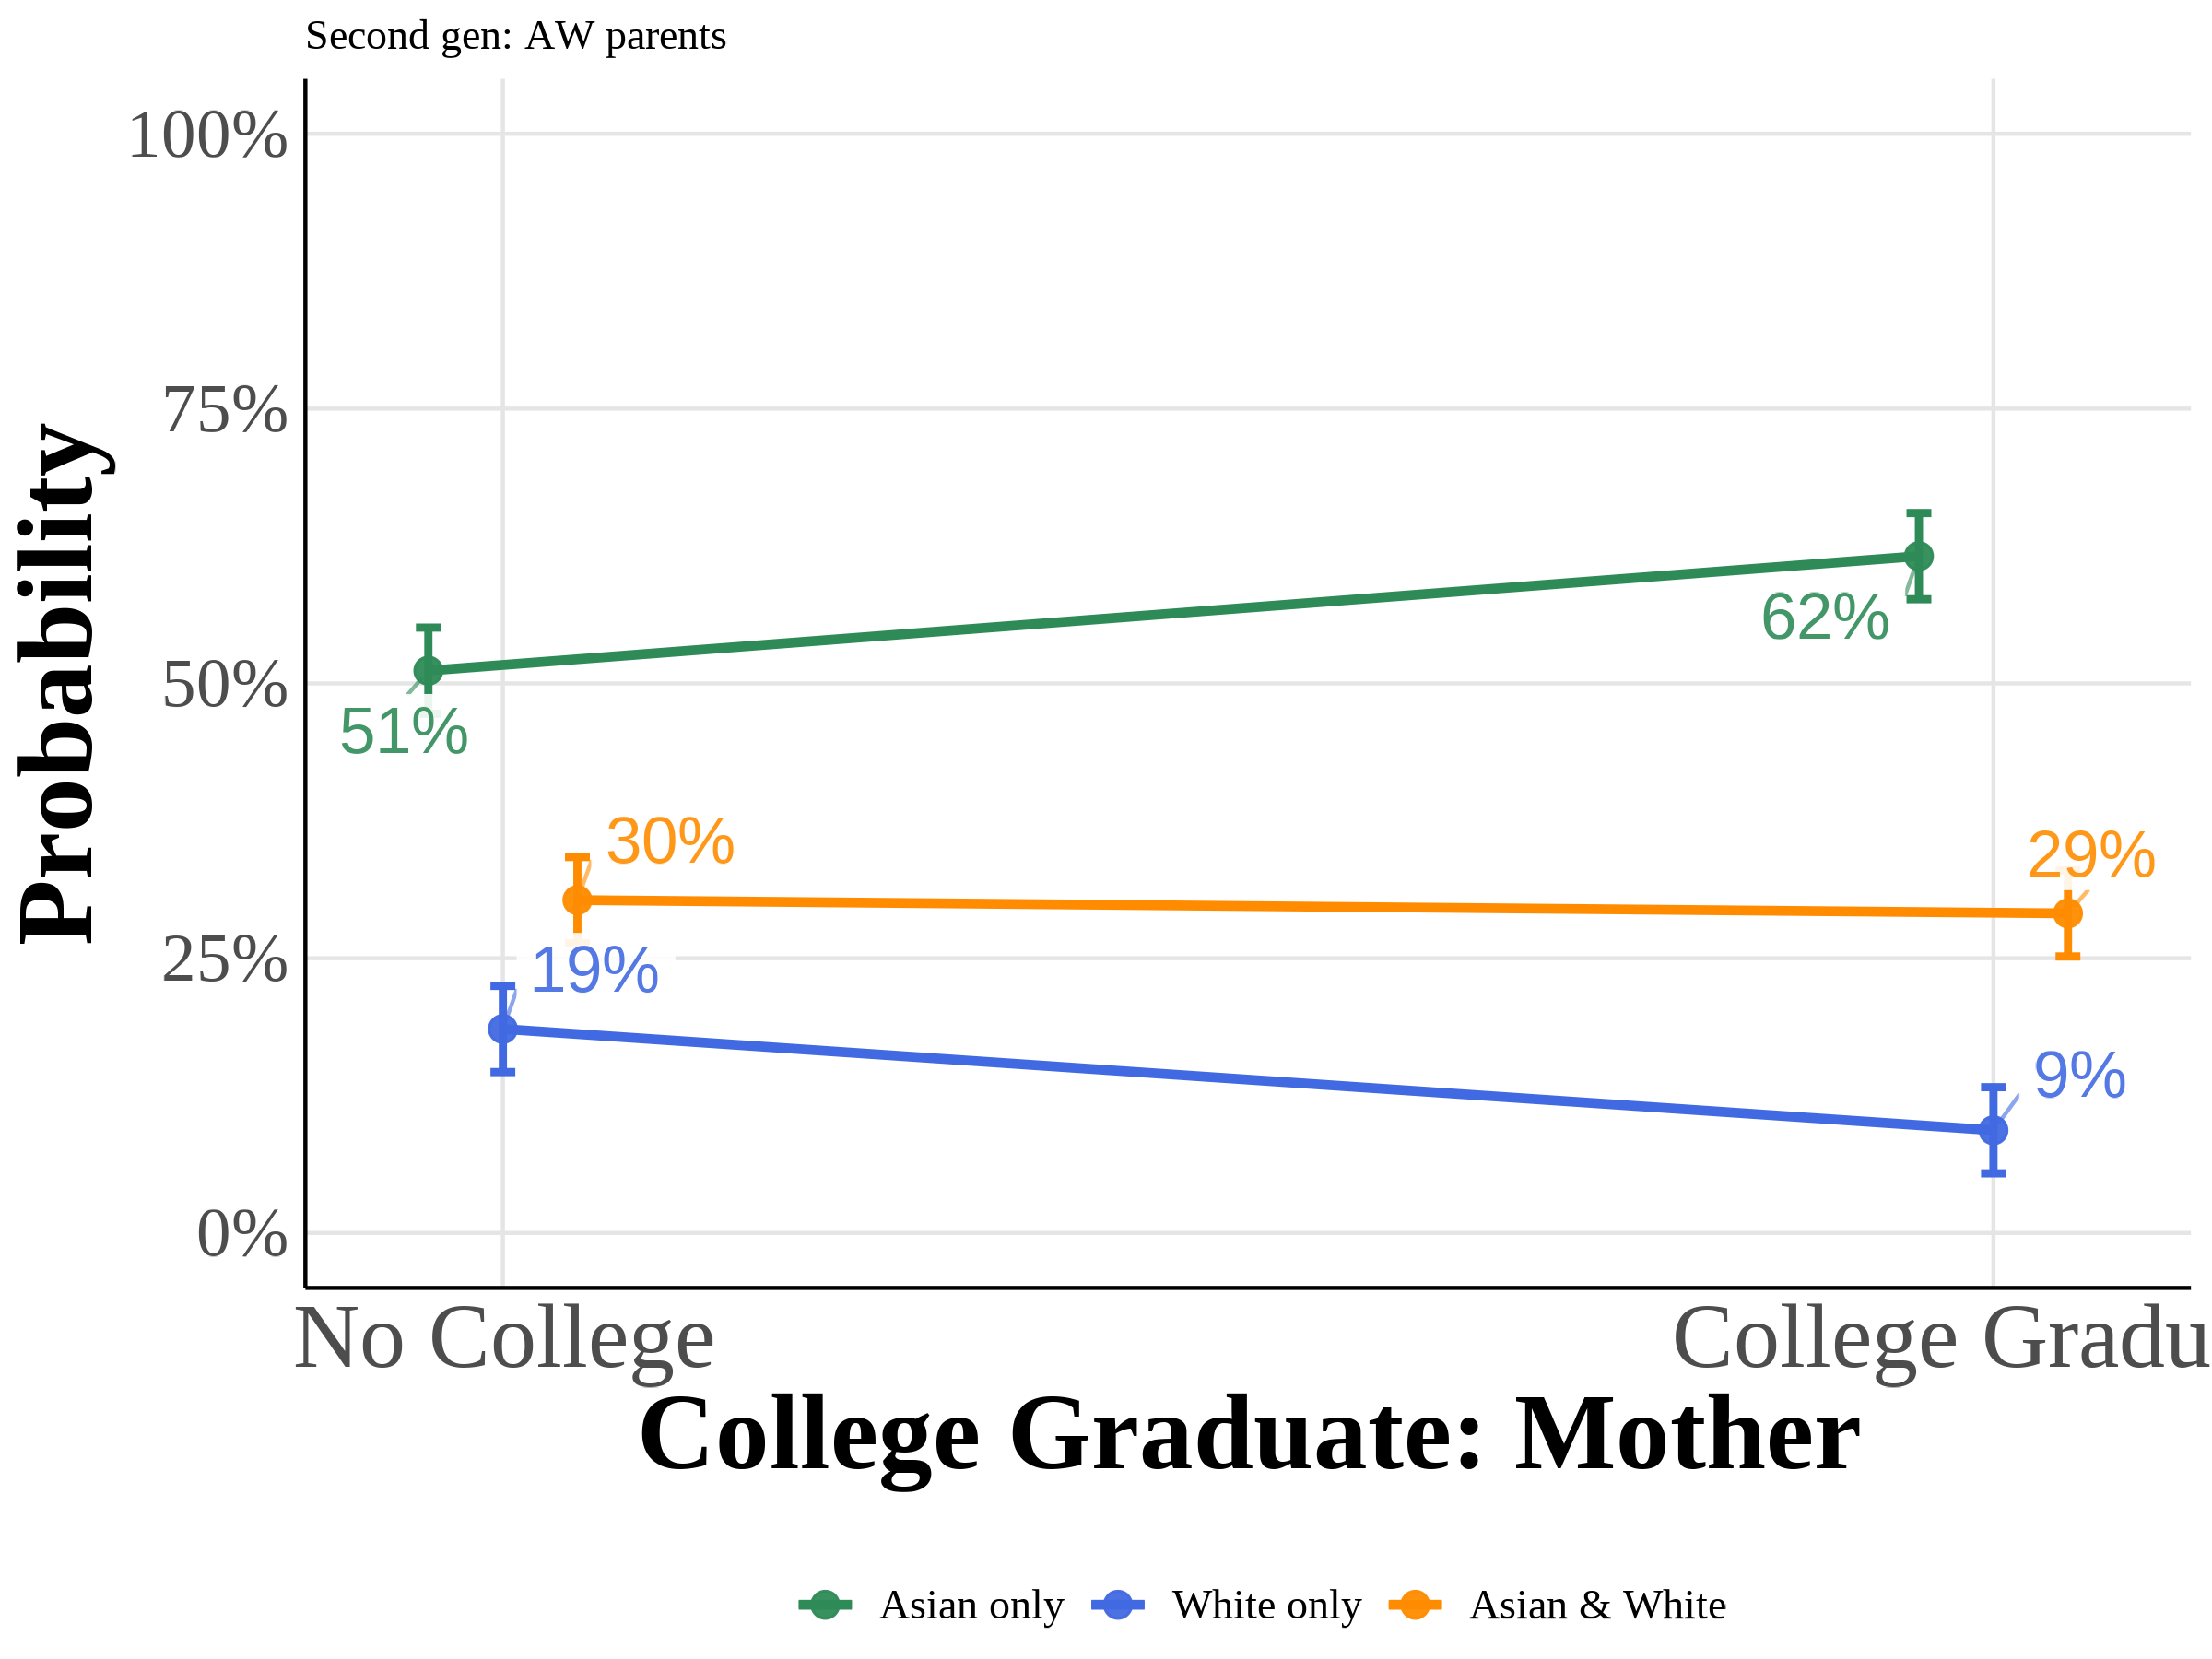
\includegraphics[width=1\linewidth]{simple_pp_MomGradCollege_second_aw.png}
\end{subfigure}
\hfill
\begin{subfigure}{.48\textwidth}
\caption{College Graduate: Father}
\centering
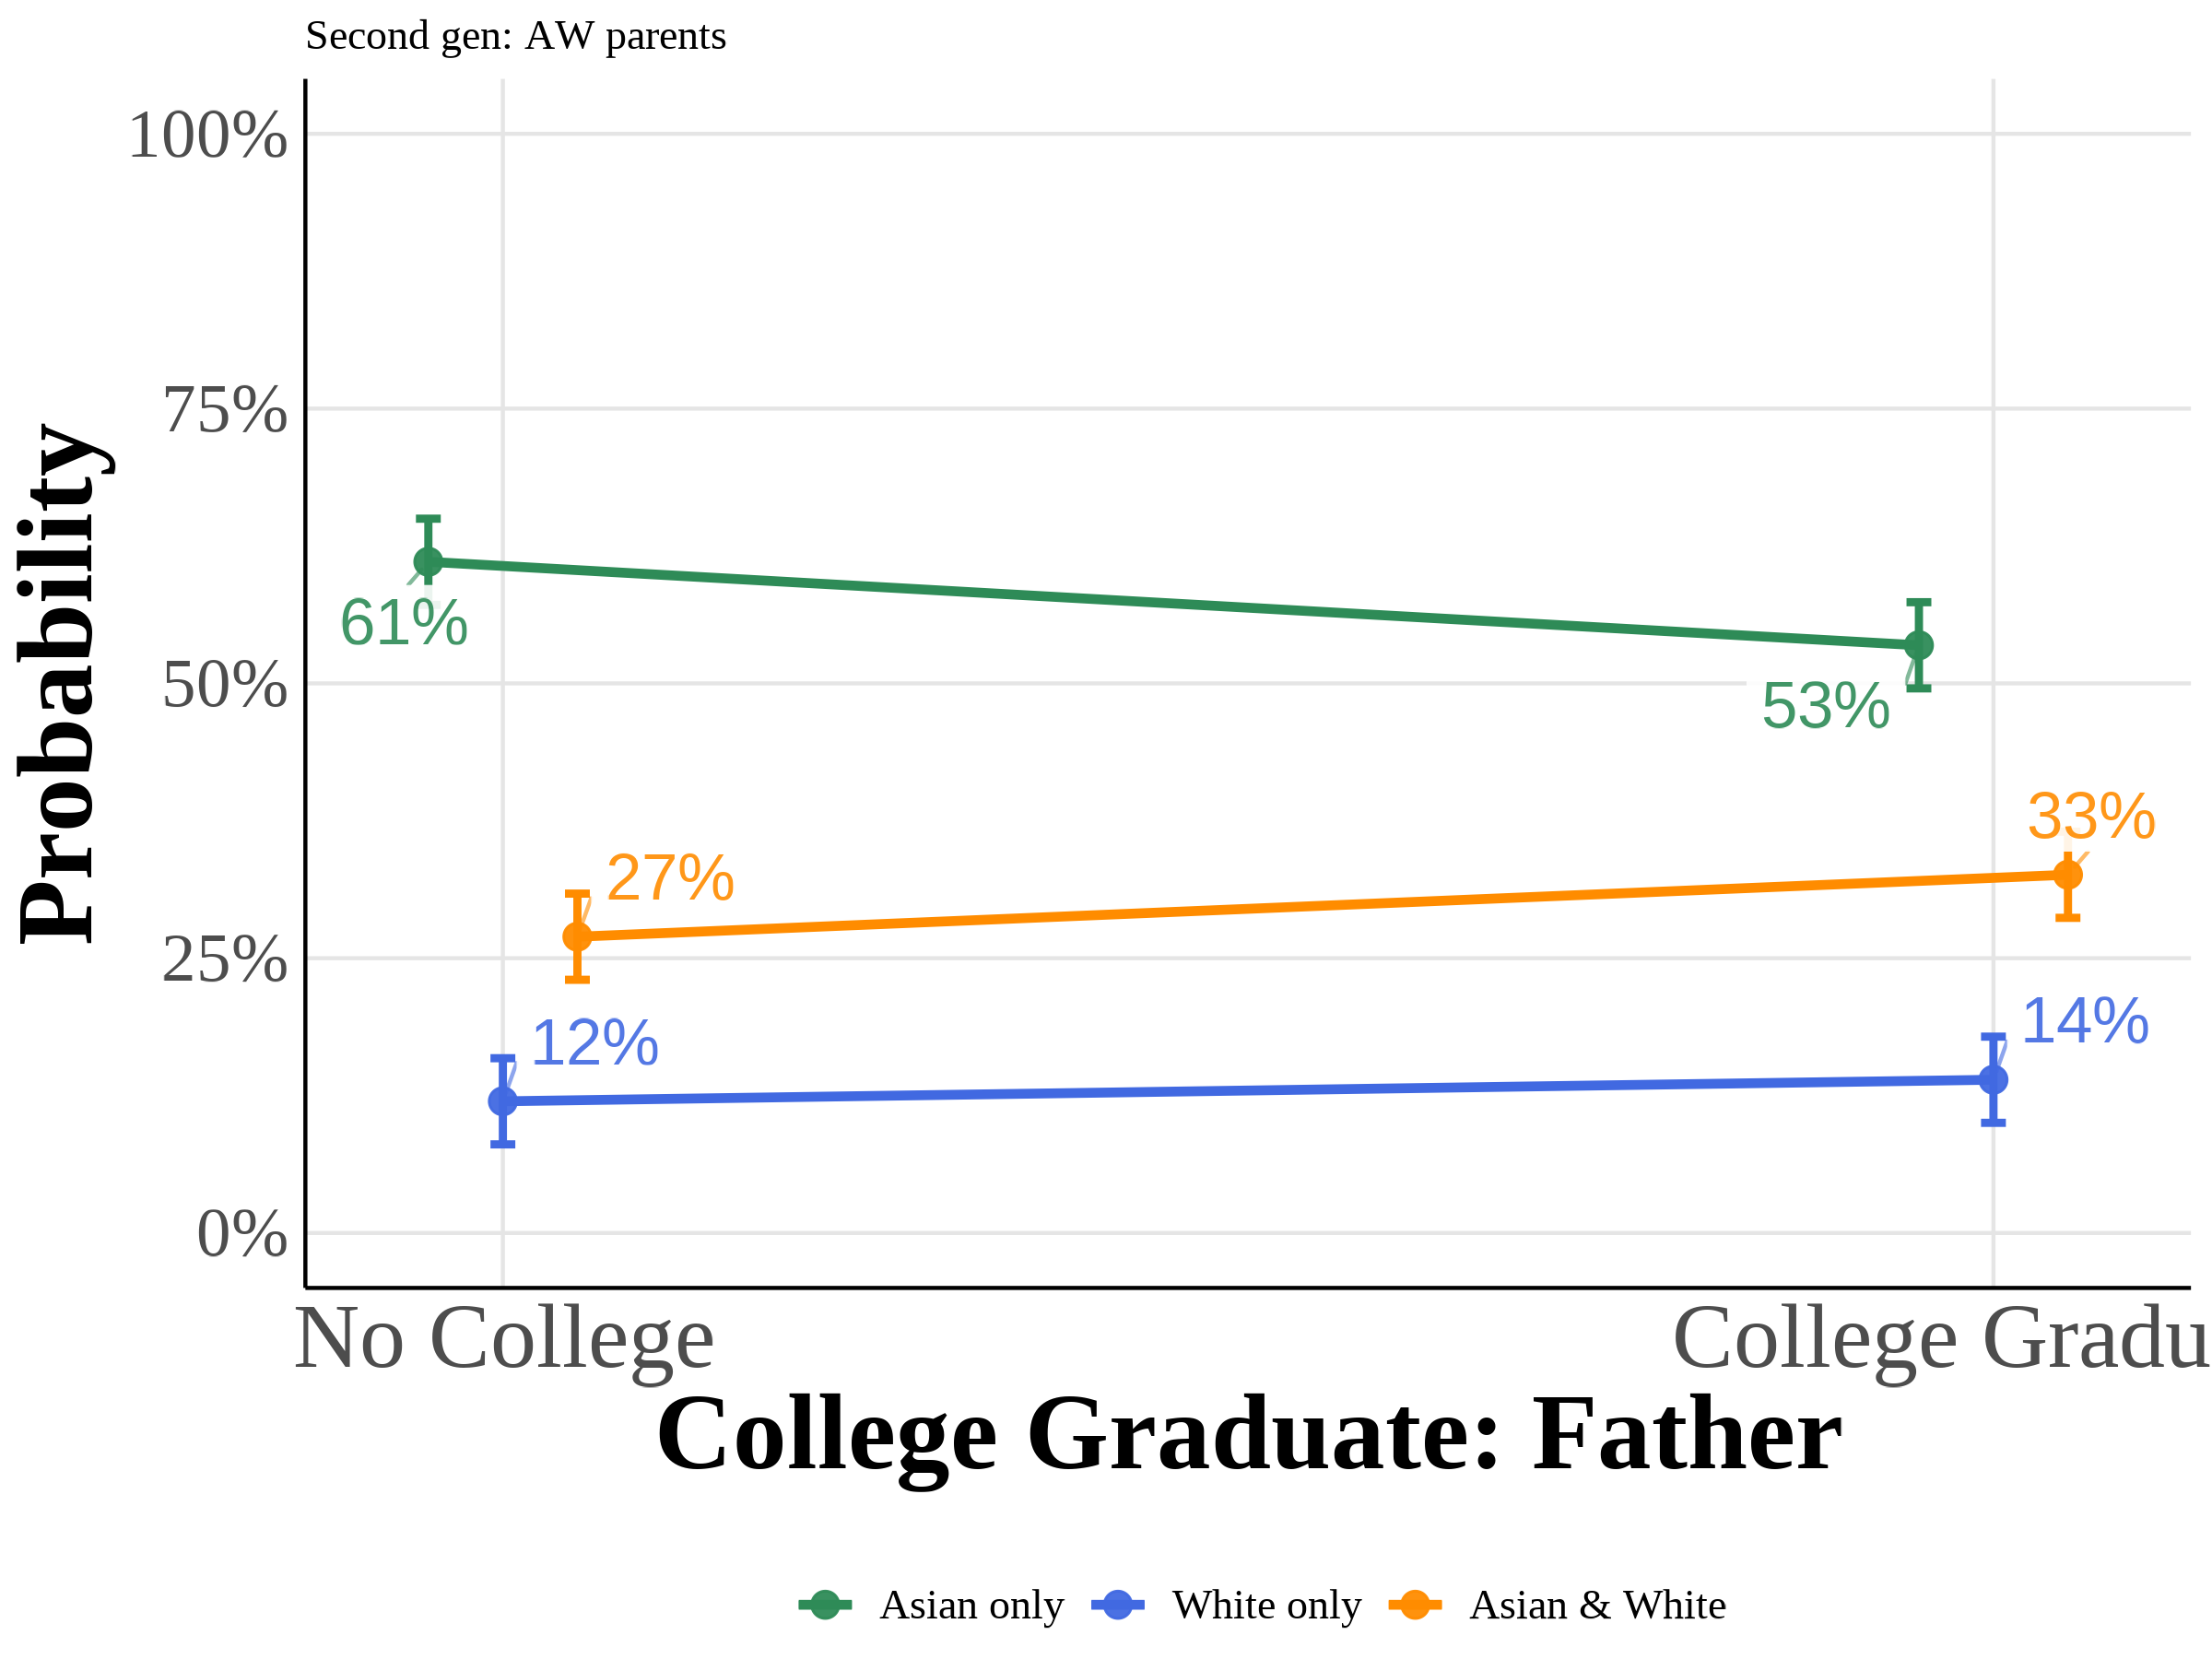
\includegraphics[width=1\linewidth]{simple_pp_DadGradCollege_second_aw.png}
\end{subfigure}

\caption*{\footnotesize{This figure shows predicted probabilities from estimating equation (\ref{eq:multinomial_logit}) using a multinomial logit model for the subsample of second-generation Asian Americans with Asian fathers and White mothers. The model estimates the probability of choosing ``Asian only'', ``White only'', or ``Asian and White'' racial identification as a function of anti-Asian bias, gender, and parental education. I include region $\times$ year fixed effects with controls for quartic age and local Asian population share. All other variables are held at their sample means.}}
\end{figure}
\end{center}

\pagebreak
\newpage

\begin{center}
\begin{figure}[!htb]
\centering
\caption{Multinomial Logit Model: Predicted Probabilities of Racial Identity Choice by Key Covariates (Second-Generation Asian Americans with White Fathers and Asian Mothers)}
\label{fig:pp-second-wa}

\begin{subfigure}{.48\textwidth}
\caption{Anti-Asian Bias}
\centering
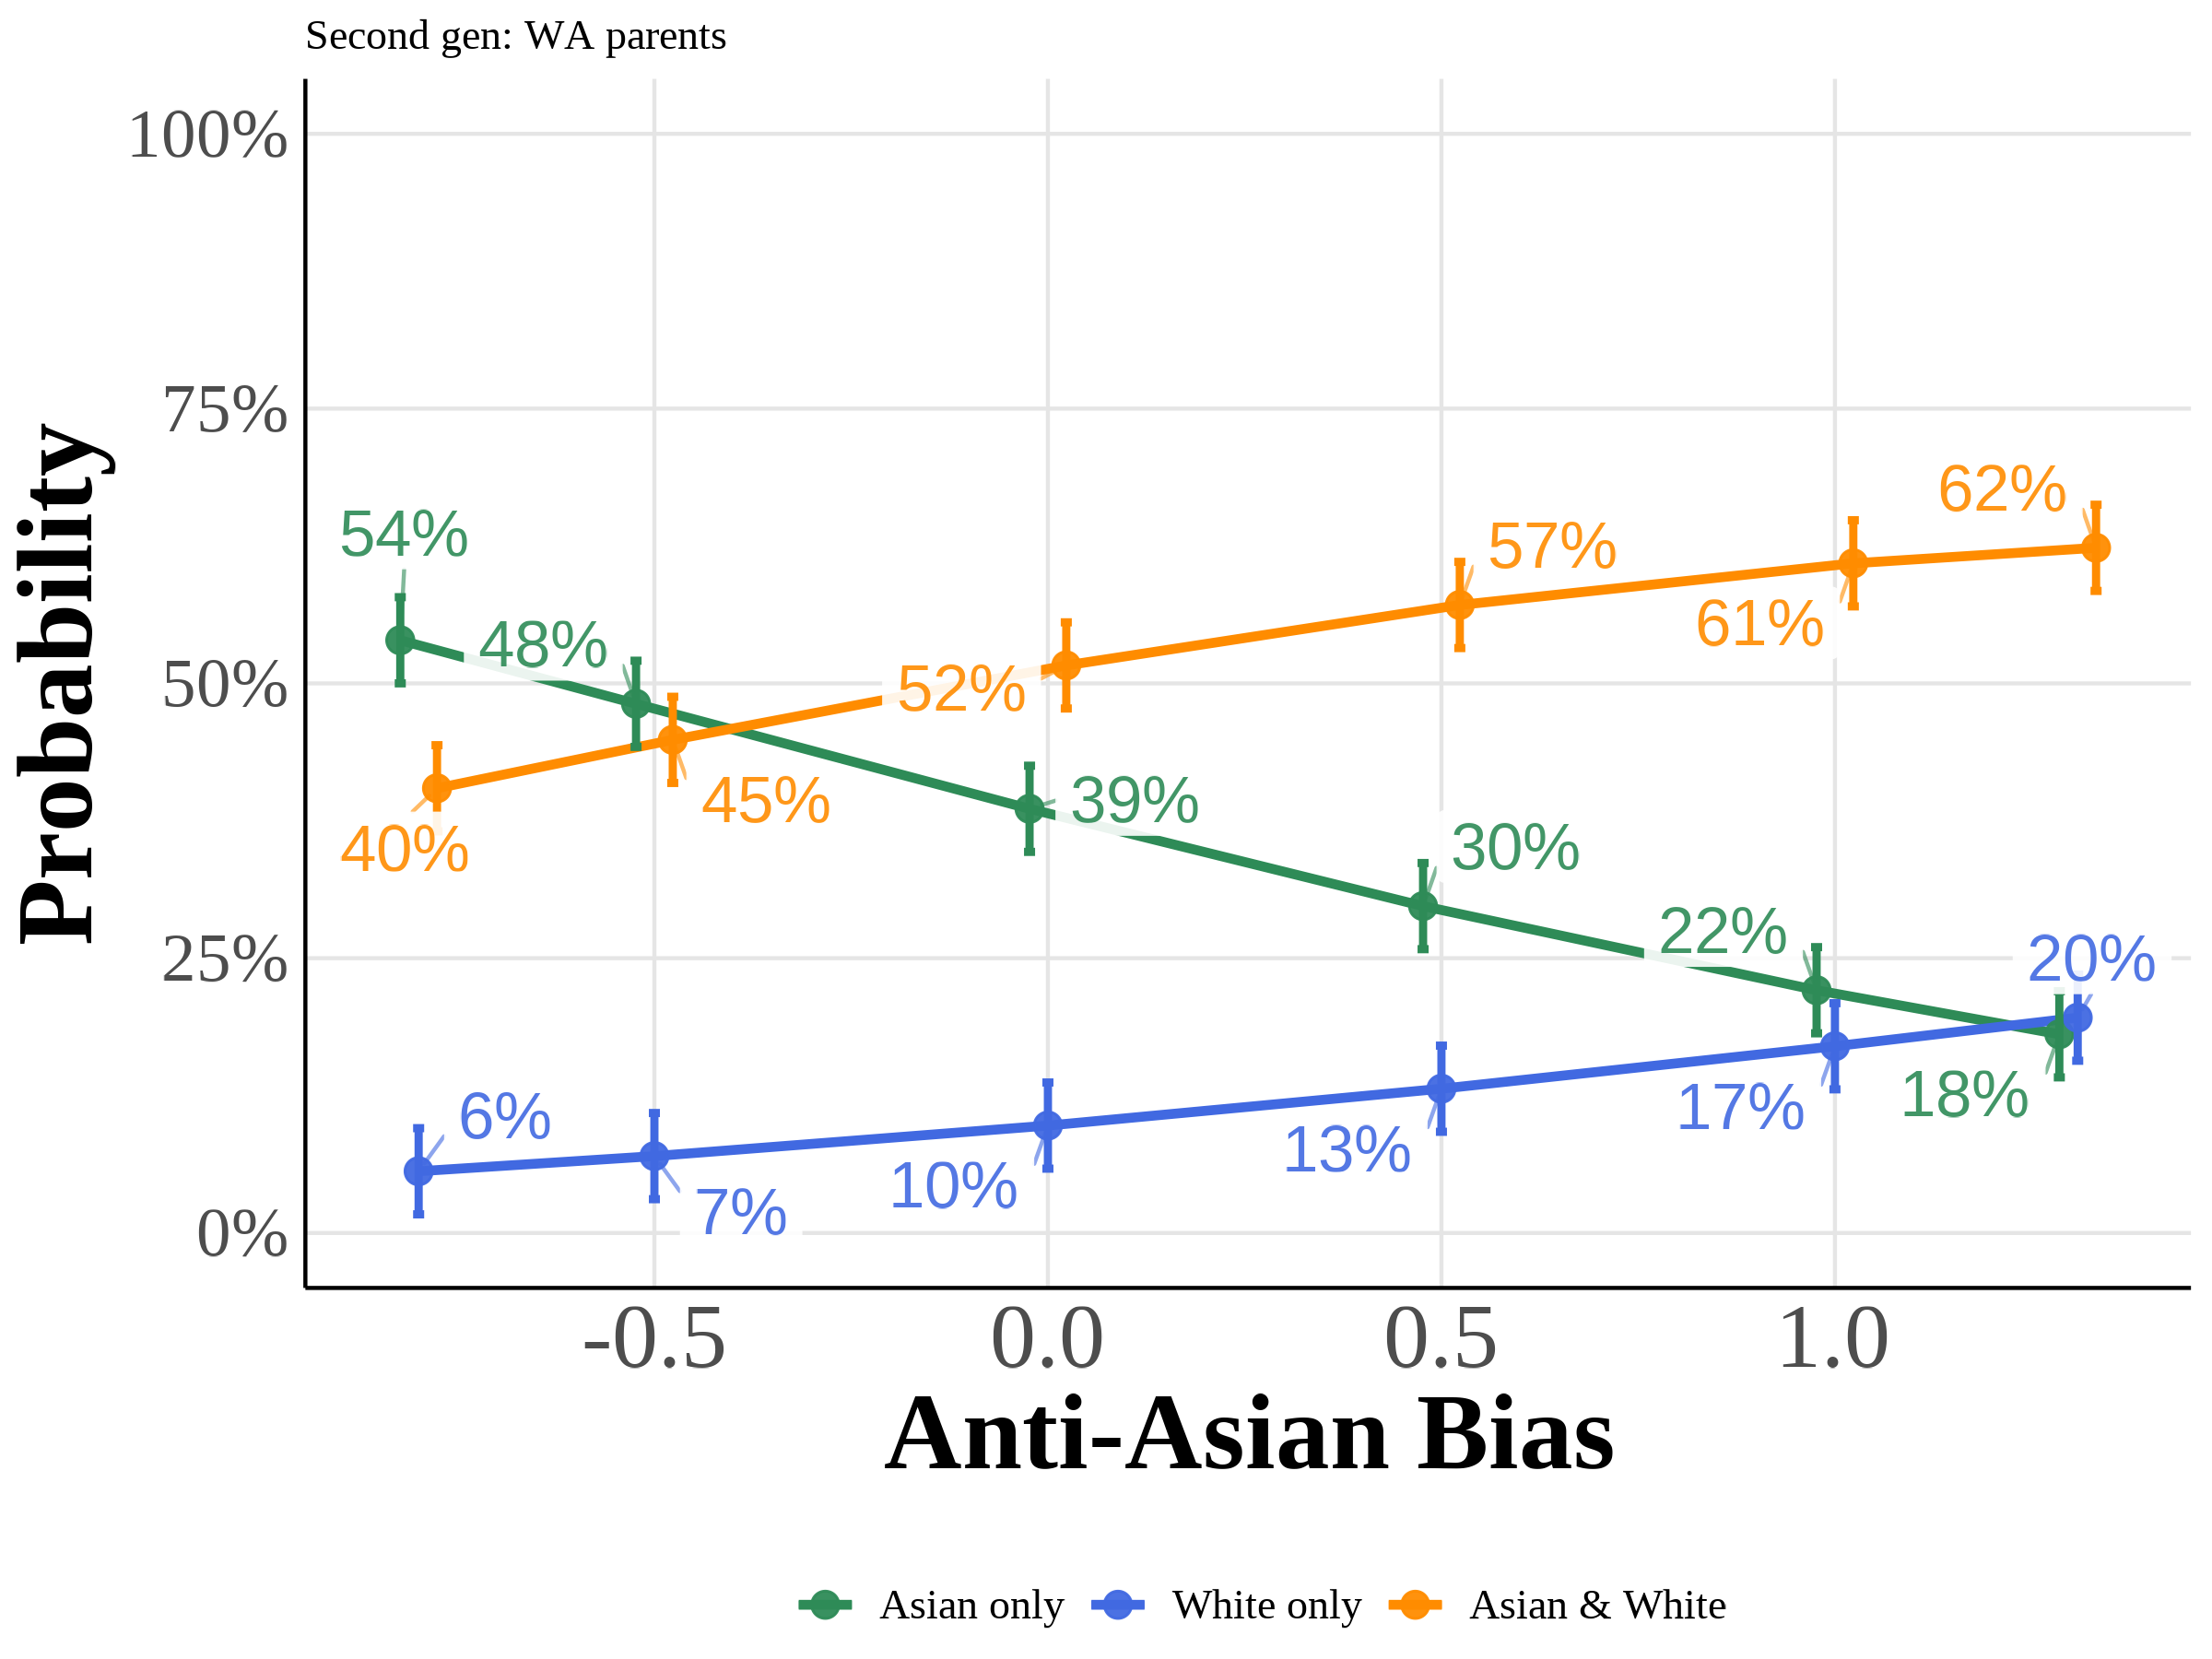
\includegraphics[width=1\linewidth]{simple_pp_value_second_wa.png}
\end{subfigure}
\hfill
\begin{subfigure}{.48\textwidth}
\caption{Female}
\centering
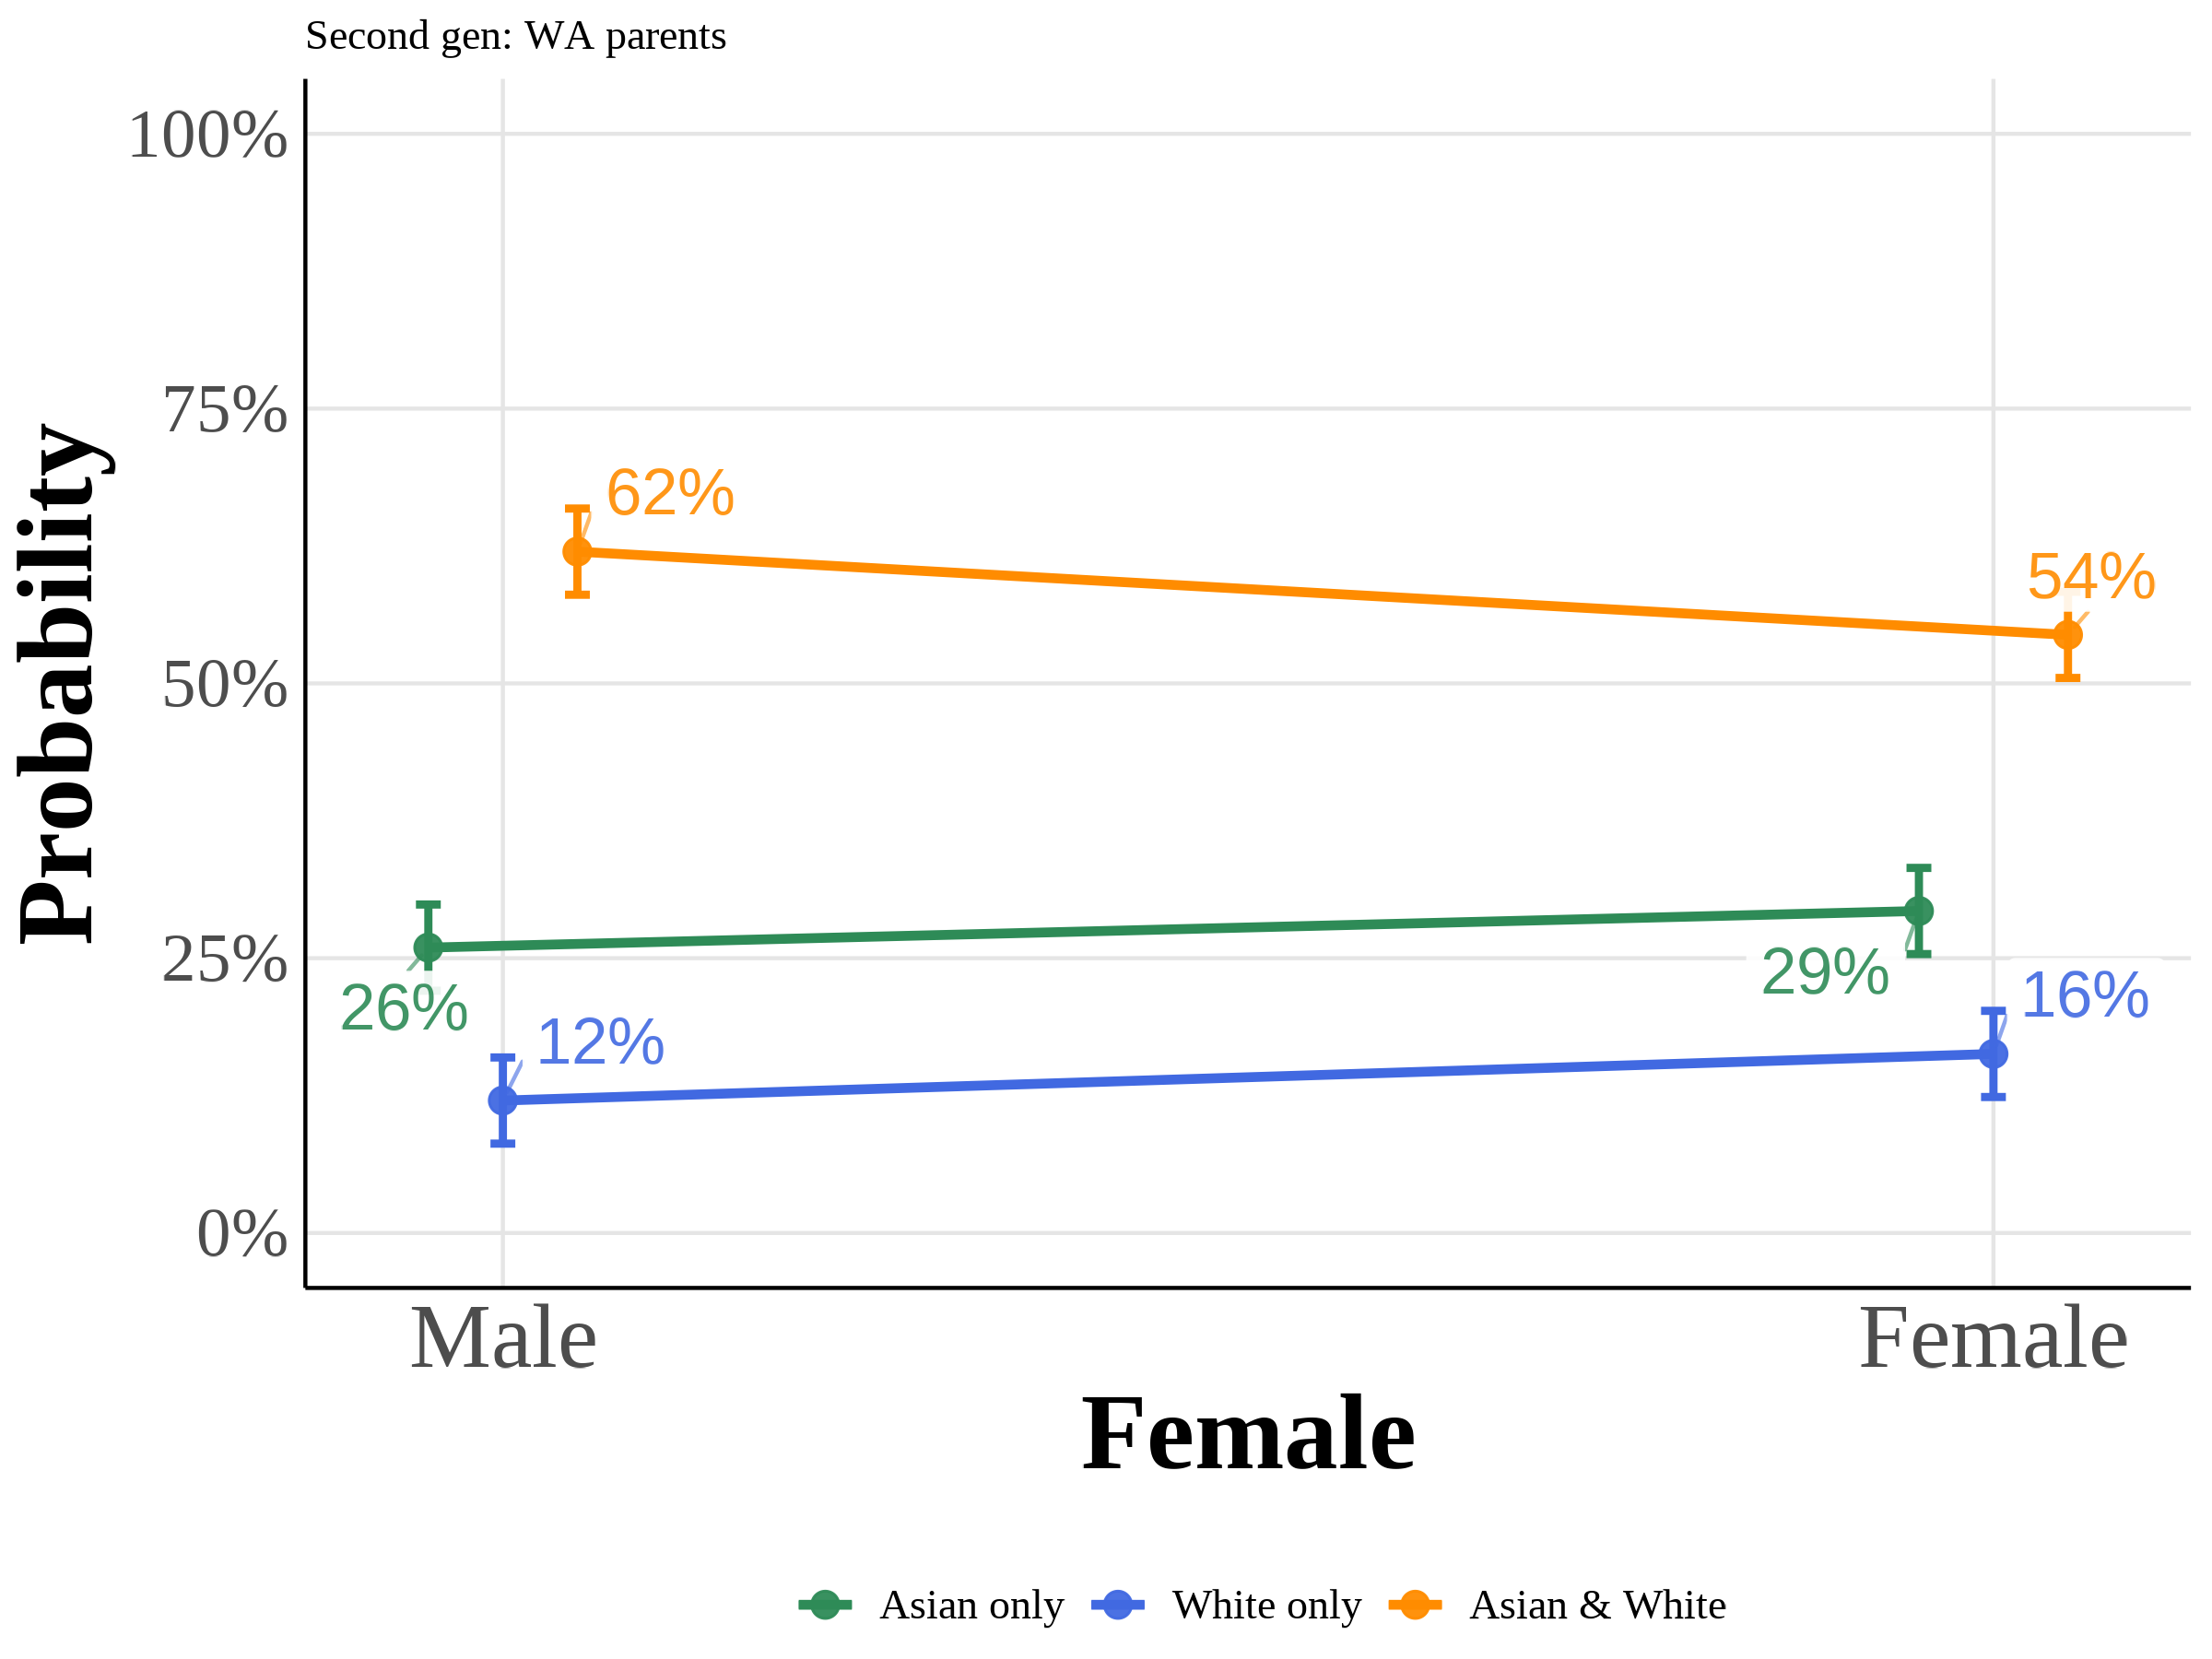
\includegraphics[width=1\linewidth]{simple_pp_Female_second_wa.png}
\end{subfigure}

\vspace{0.5cm}

\begin{subfigure}{.48\textwidth}
\caption{College Graduate: Mother}
\centering
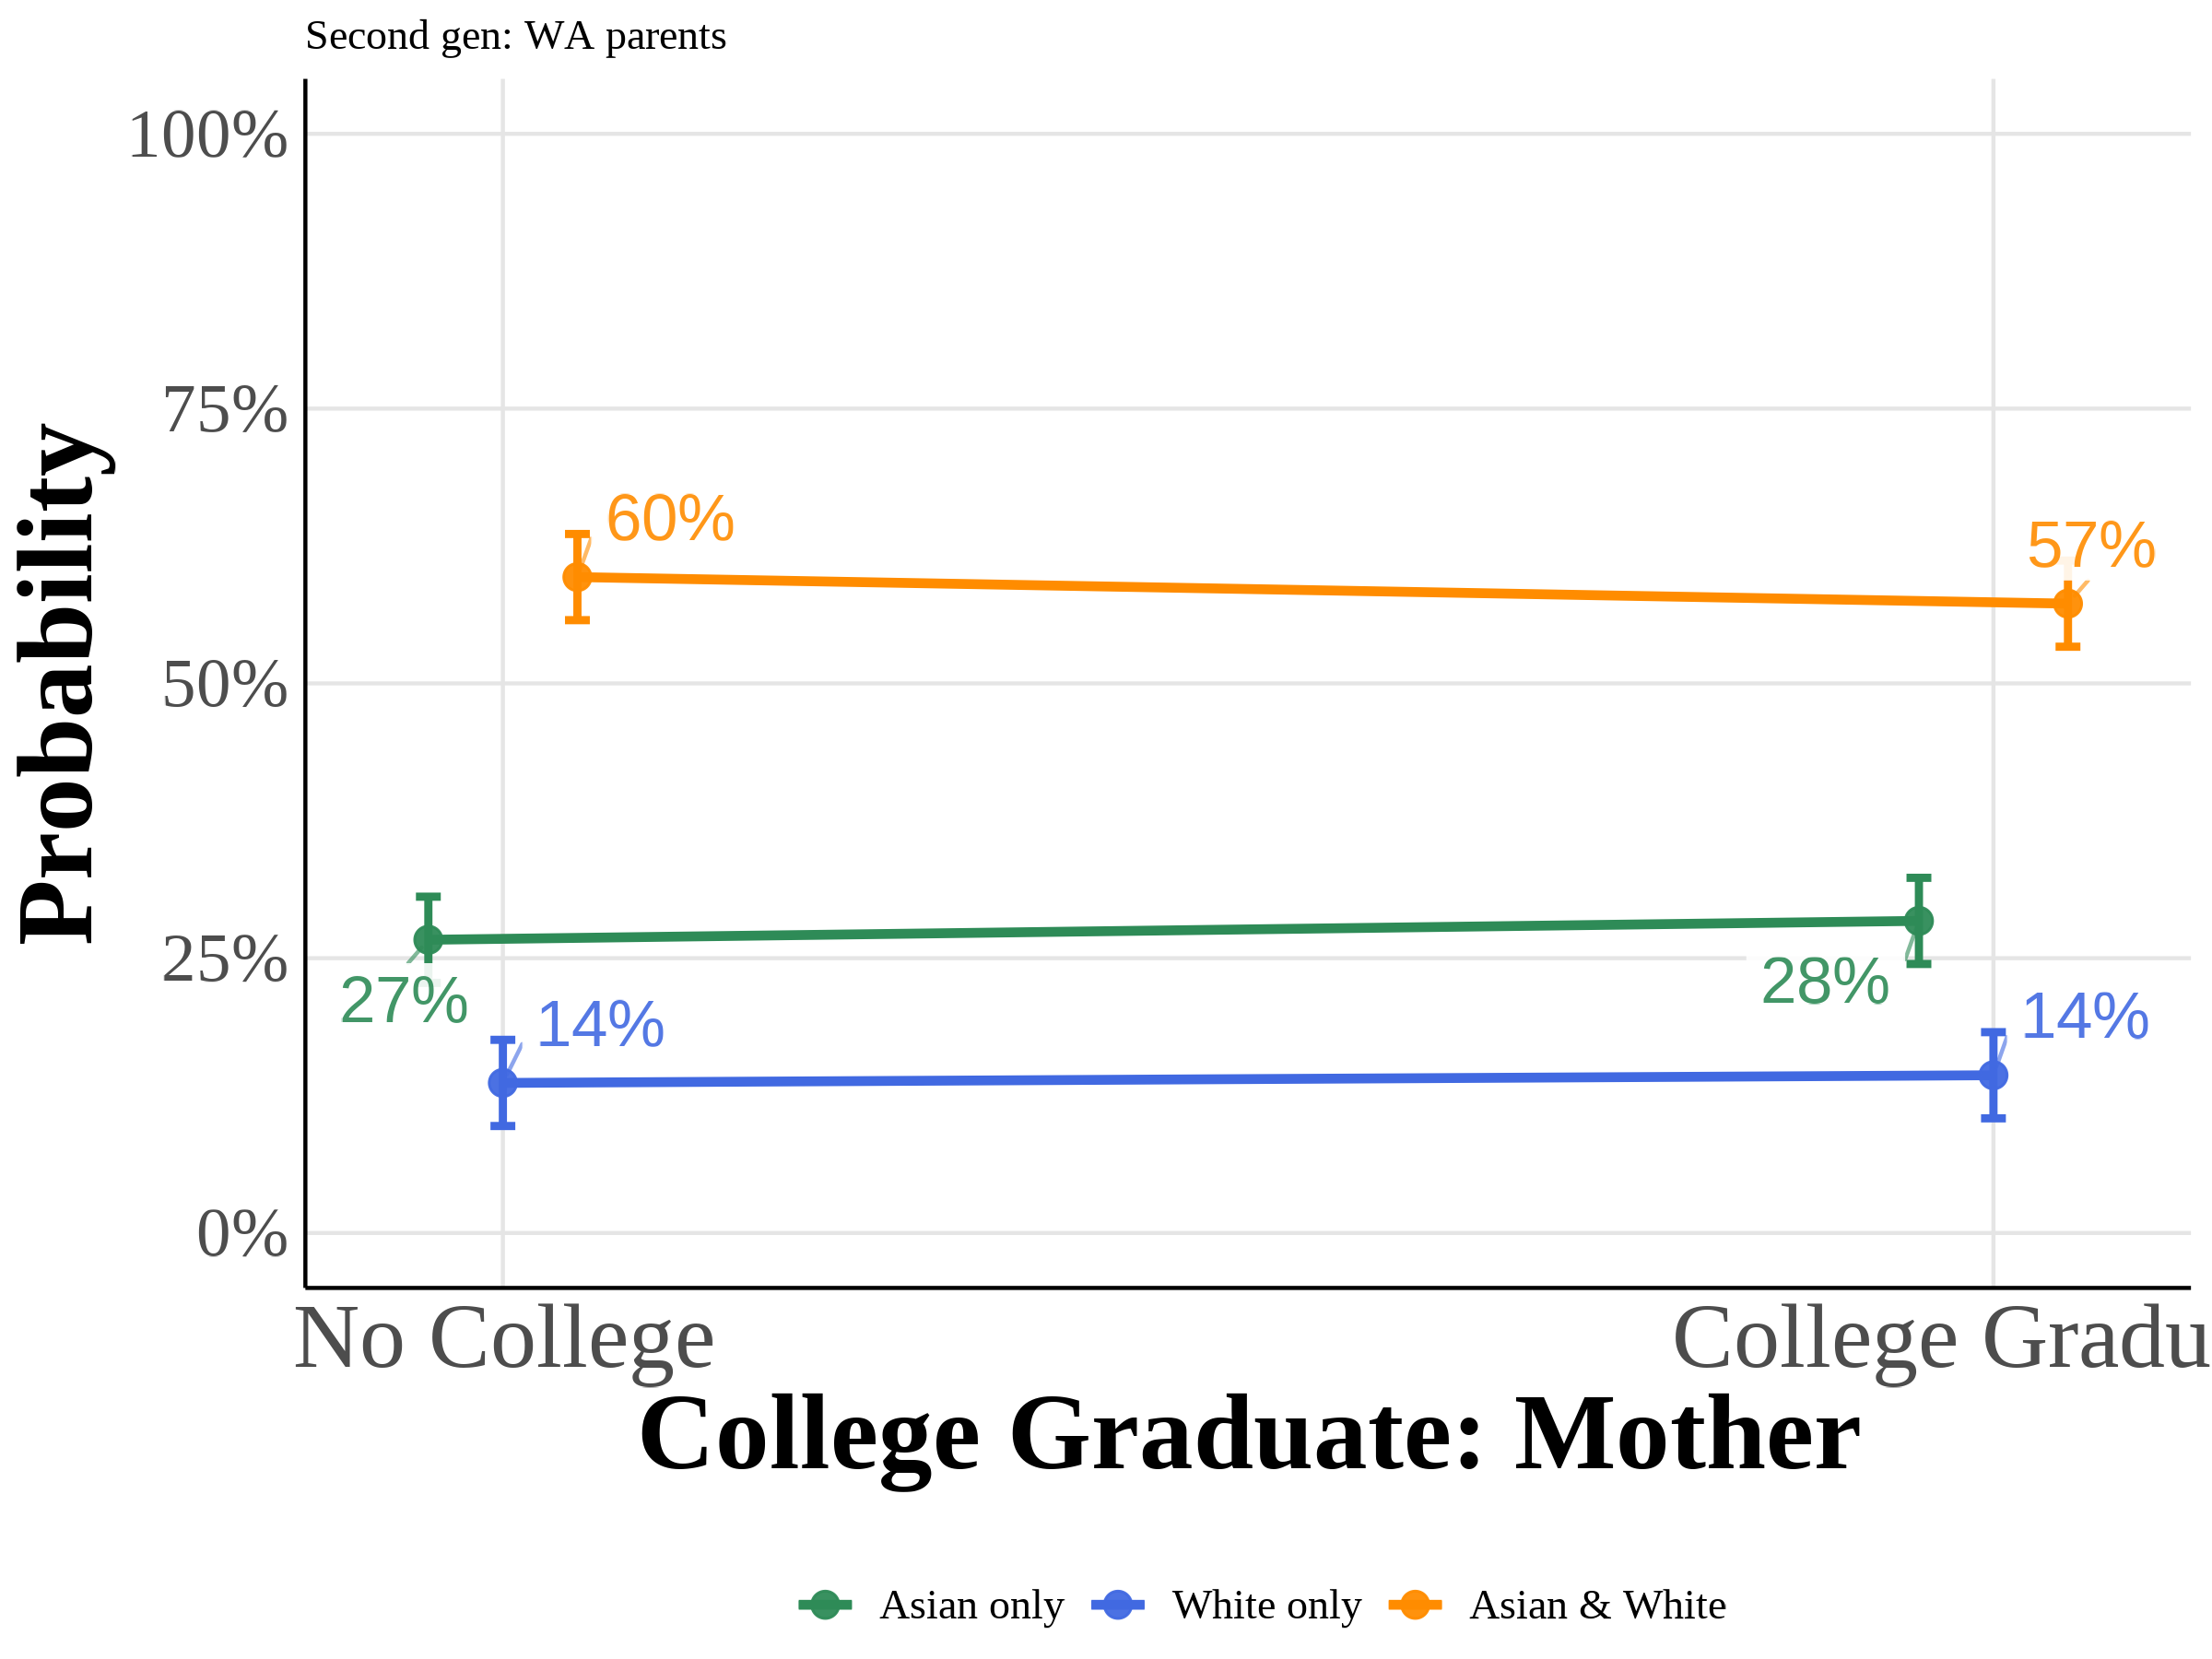
\includegraphics[width=1\linewidth]{simple_pp_MomGradCollege_second_wa.png}
\end{subfigure}
\hfill
\begin{subfigure}{.48\textwidth}
\caption{College Graduate: Father}
\centering
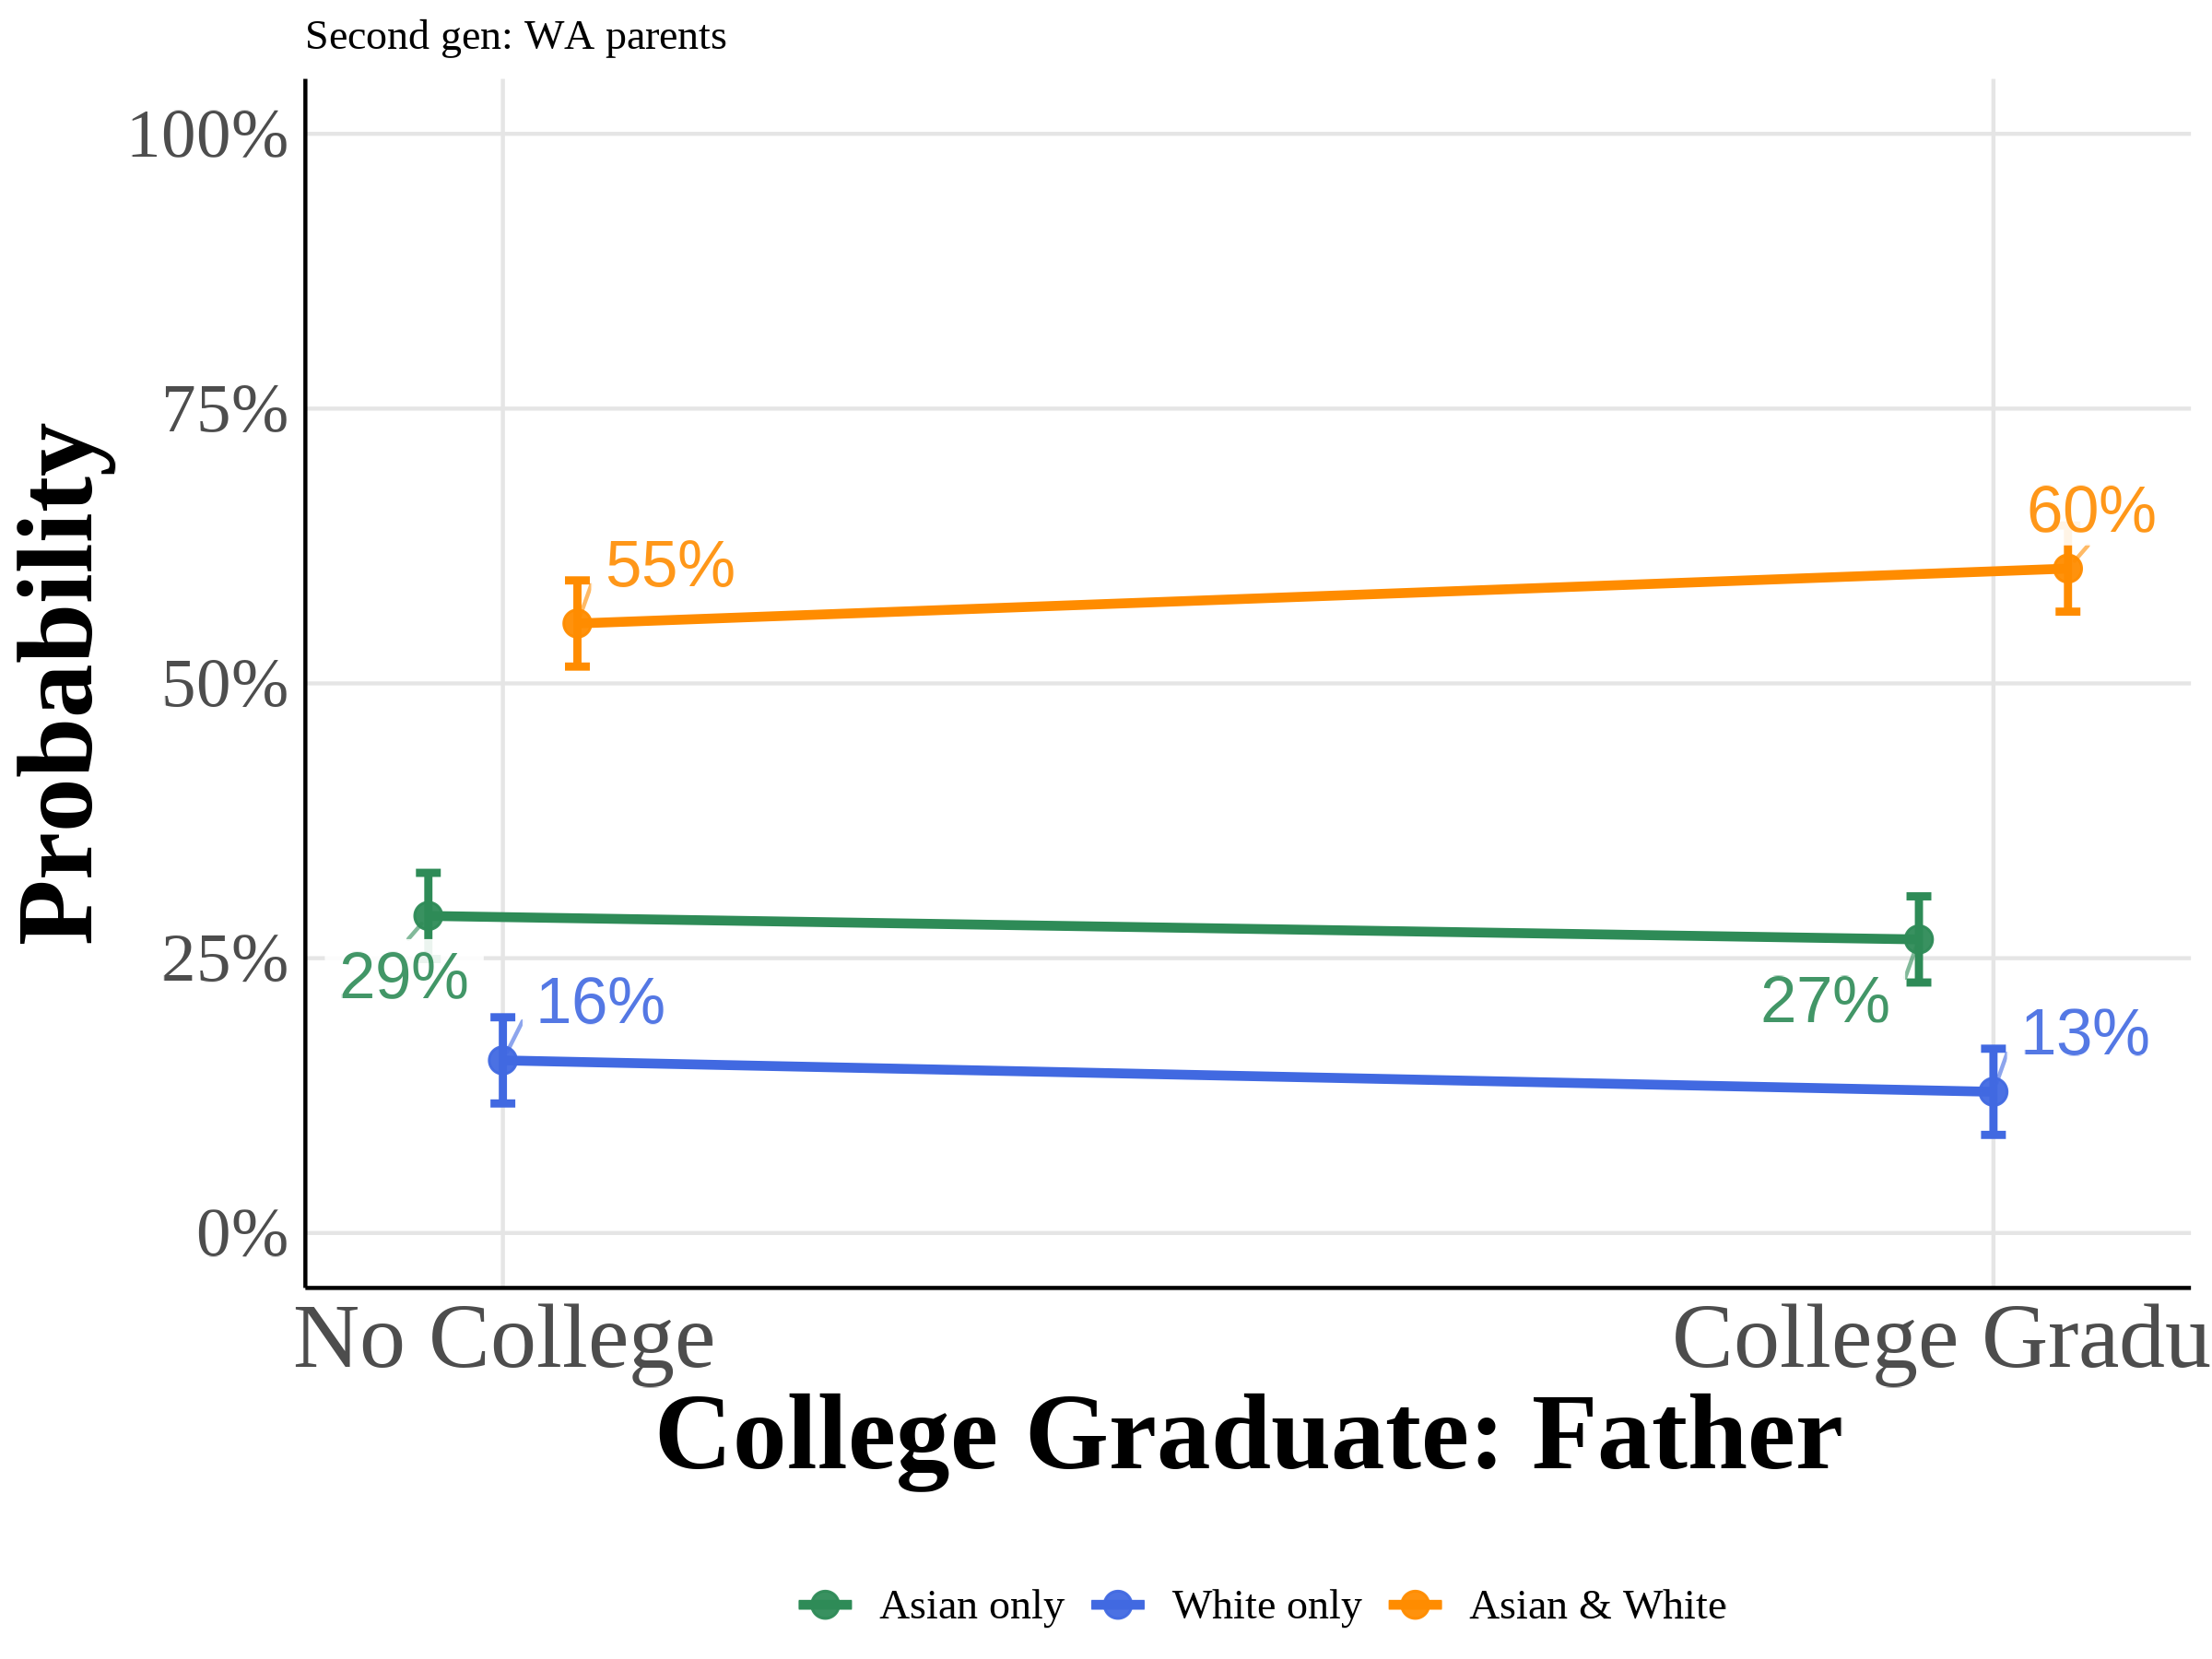
\includegraphics[width=1\linewidth]{simple_pp_DadGradCollege_second_wa.png}
\end{subfigure}

\caption*{\footnotesize{This figure shows predicted probabilities from estimating equation (\ref{eq:multinomial_logit}) using a multinomial logit model for the subsample of second-generation Asian Americans with Asian fathers and White mothers. The model estimates the probability of choosing ``Asian only'', ``White only'', or ``Asian and White'' racial identification as a function of anti-Asian bias, gender, and parental education. I include region $\times$ year fixed effects with controls for quartic age and local Asian population share. All other variables are held at their sample means.}}
\end{figure}
\end{center}

\pagebreak
\newpage

% % Marginal Effects: Second Generation by Parental Type (AW and WA)
% \begin{center}
% \begin{figure}[!htb]
% \centering
% \caption{Marginal Effects of Key Covariates on Racial Identity Choice by Parental Ancestry (Second-Generation Asian Americans)}
% \label{fig:marginal-effects-second-parental}

% \begin{subfigure}{.48\textwidth}
% \caption{Asian Father-White Mother (AW)}\label{subfig:meaw}
% \centering
% 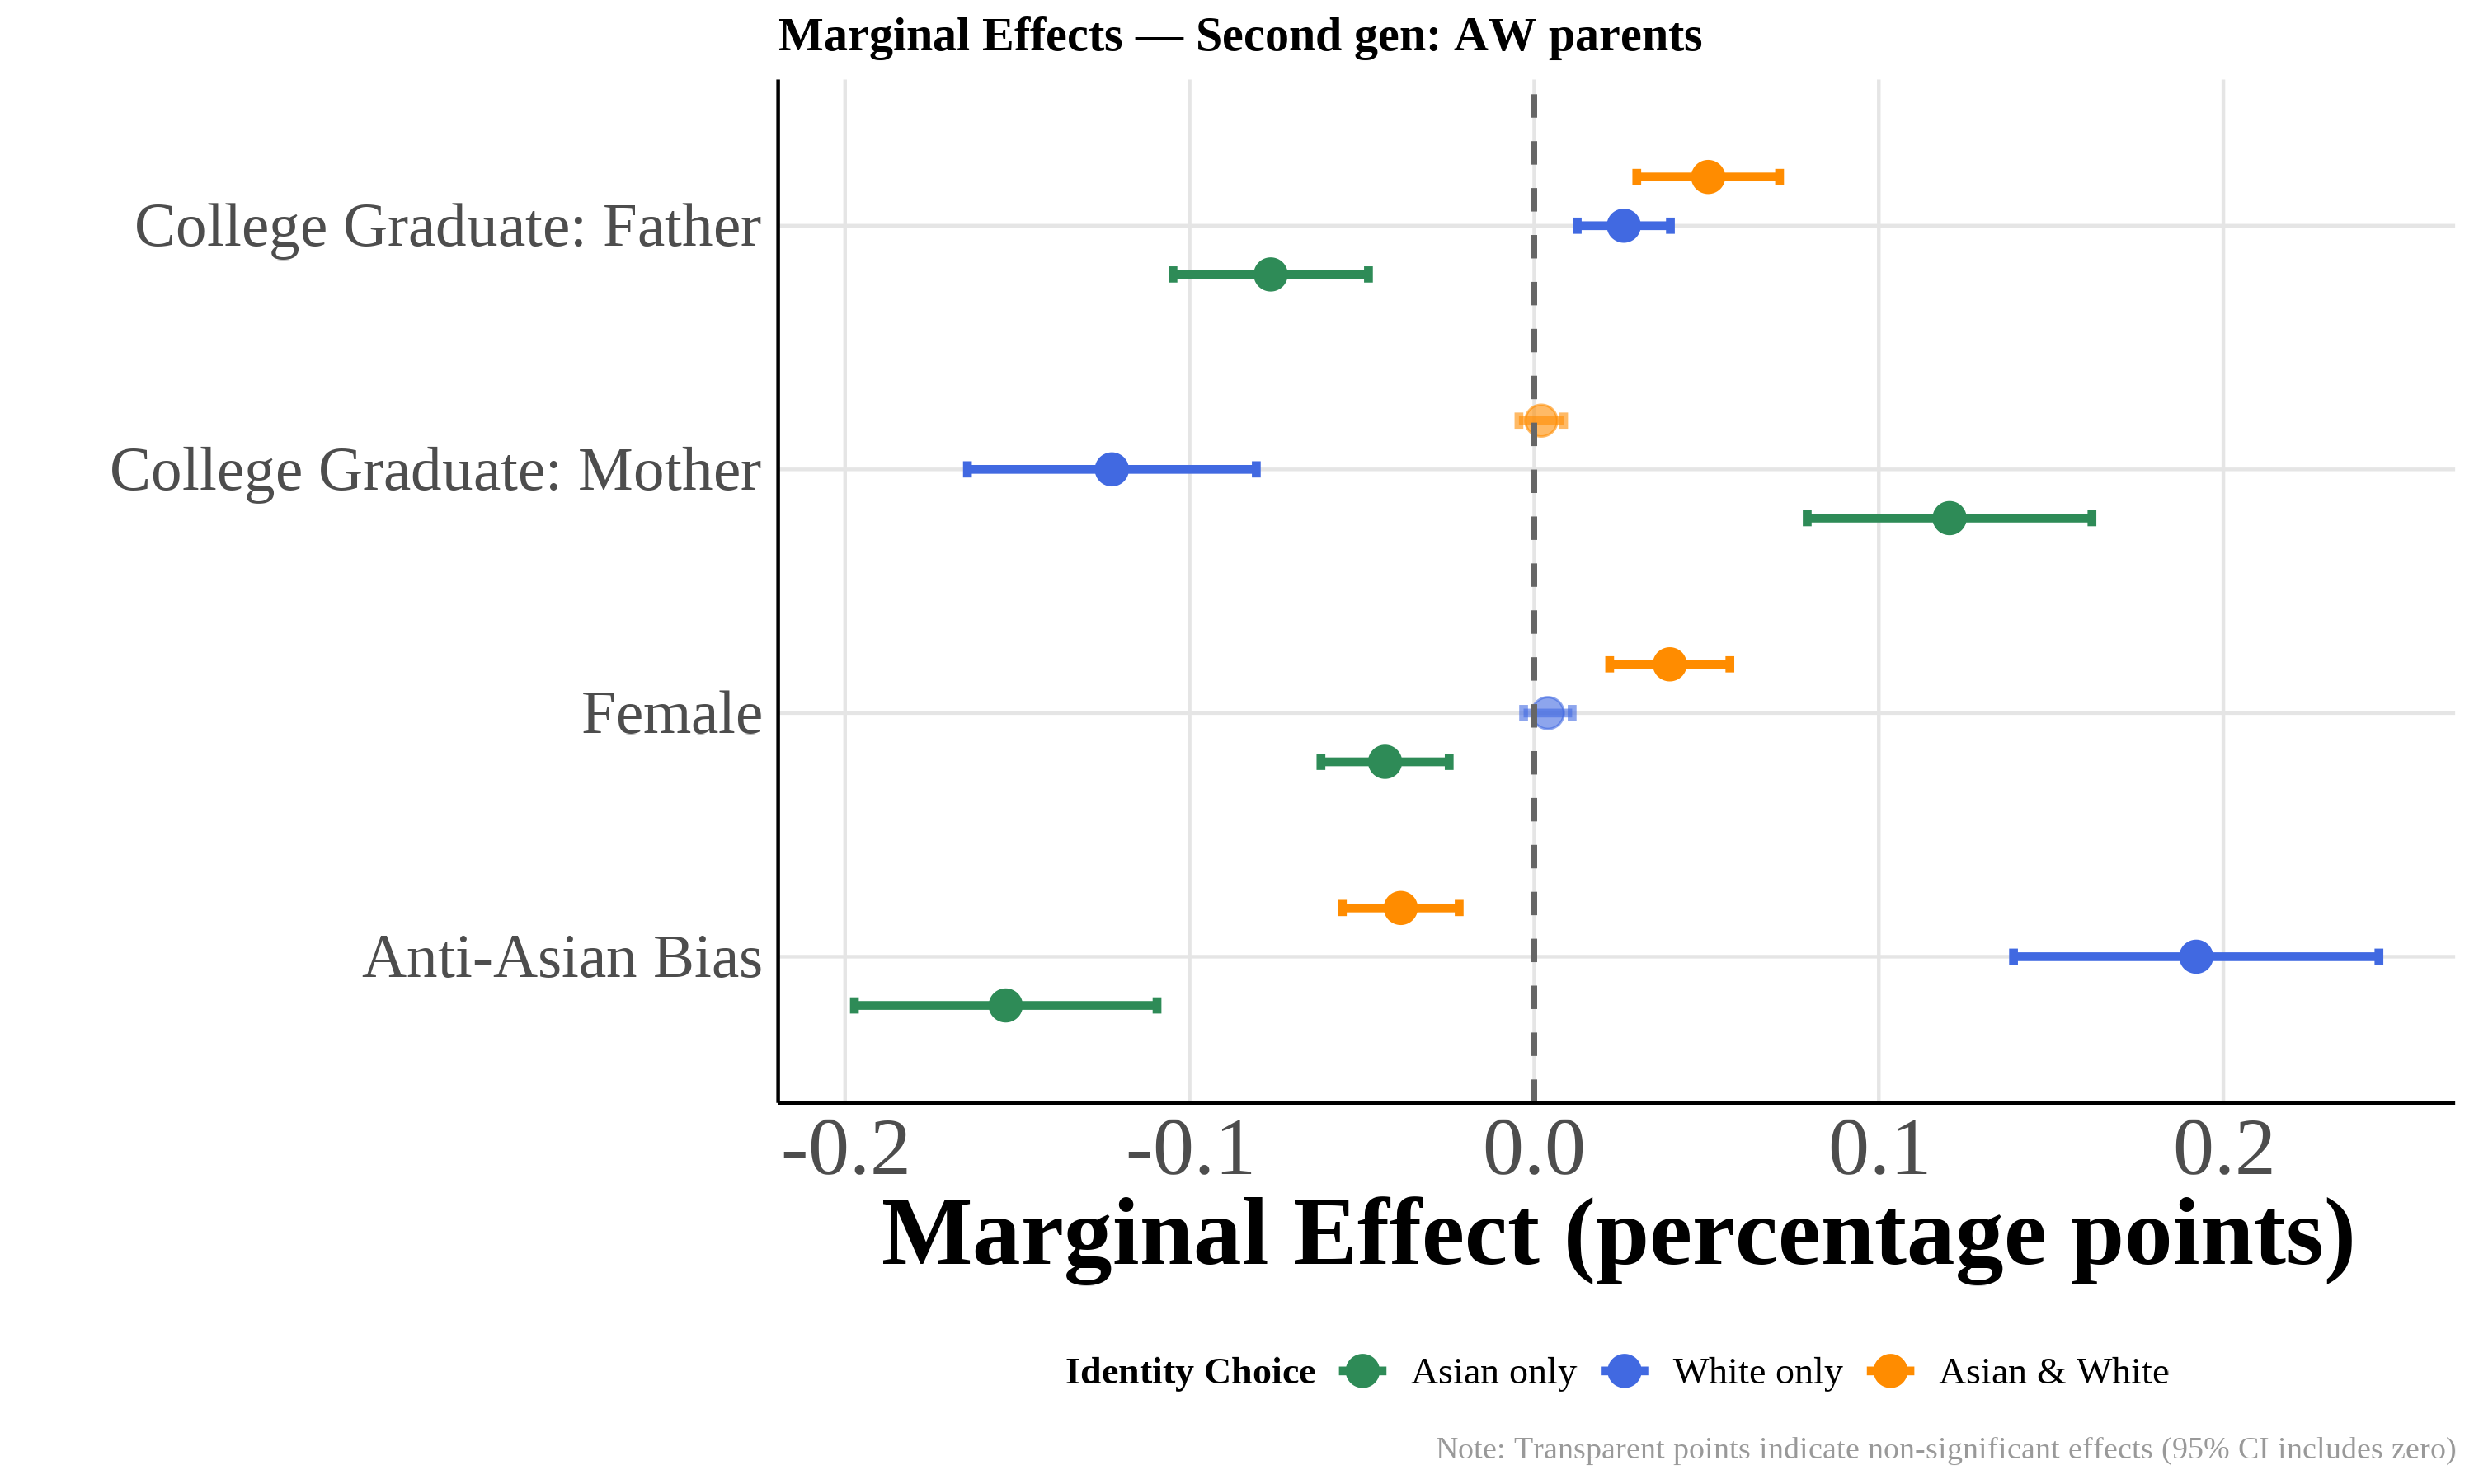
\includegraphics[width=1\linewidth]{optimized_marginal_effects_second_aw.png}
% \end{subfigure}
% \hfill
% \begin{subfigure}{.48\textwidth}
% \caption{White Father-Asian Mother (WA)}\label{subfig:mewa}
% \centering
% 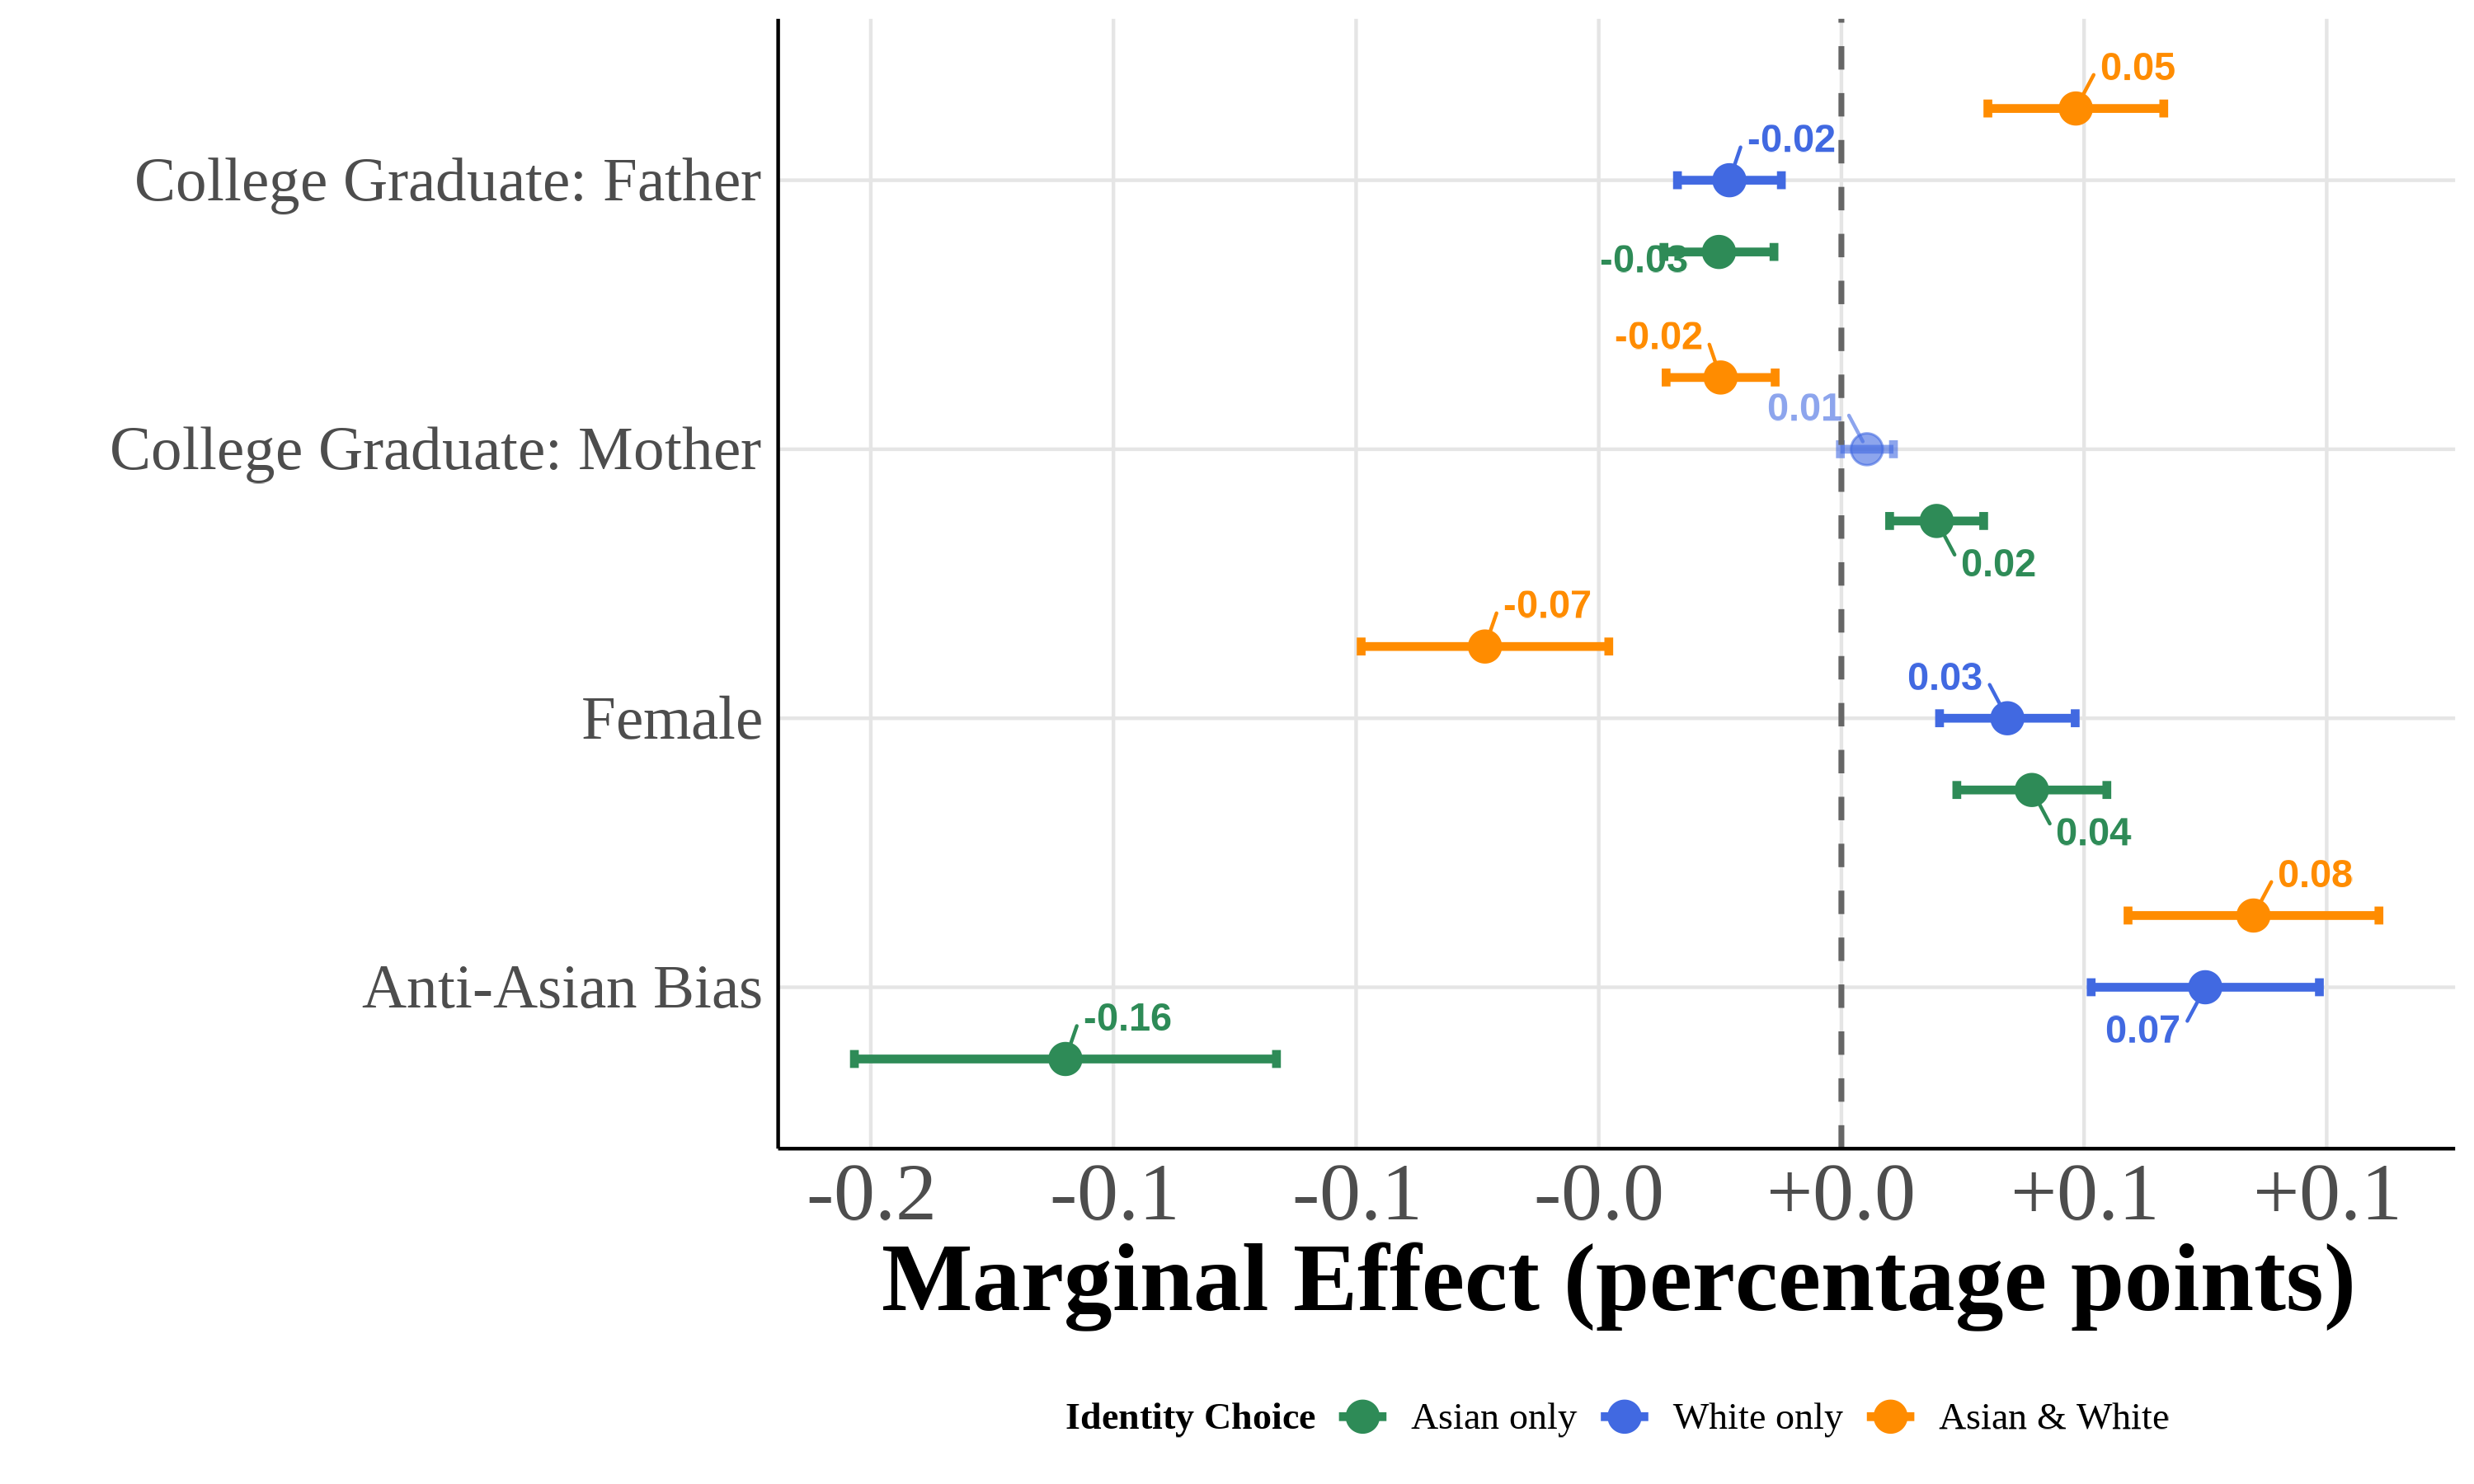
\includegraphics[width=1\linewidth]{optimized_marginal_effects_second_wa.png}
% \end{subfigure}

% \caption*{\footnotesize{This figure displays the marginal effects of key covariates on the probability of each racial identification outcome, estimated from equation (\ref{eq:multinomial_logit}) using multinomial logit models for second-generation Asian Americans by parental ancestry configuration. Marginal effects represent the change in predicted probability for a one-unit increase in the covariate (or discrete change from 0 to 1 for binary variables), holding other variables at their sample means. I include region $\times$ year fixed effects with controls for quartic age and local Asian population share. Error bars indicate 95\% confidence intervals. Second-generation Asian Americans are native-born individuals with at least one Asian-born parent.}}
% \end{figure}
% \end{center}

% \pagebreak
% \newpage

% =========================
% 41: Multinomial Model - Predicted Probabilities (Adults, AW/WA)
% =========================
\begin{center}
\begin{figure}[!htb]
\centering
\caption{Multinomial Logit Model: Predicted Probabilities of Racial Identity Choice by Key Covariates (Second Generation Adults, AW/WA)}
\label{fig:pp-secondgen-adults-aw-wa}

% Top row: Anti-Asian Bias and Female
\begin{subfigure}{.48\textwidth}
\caption{Anti-Asian Bias (AW)}
\centering
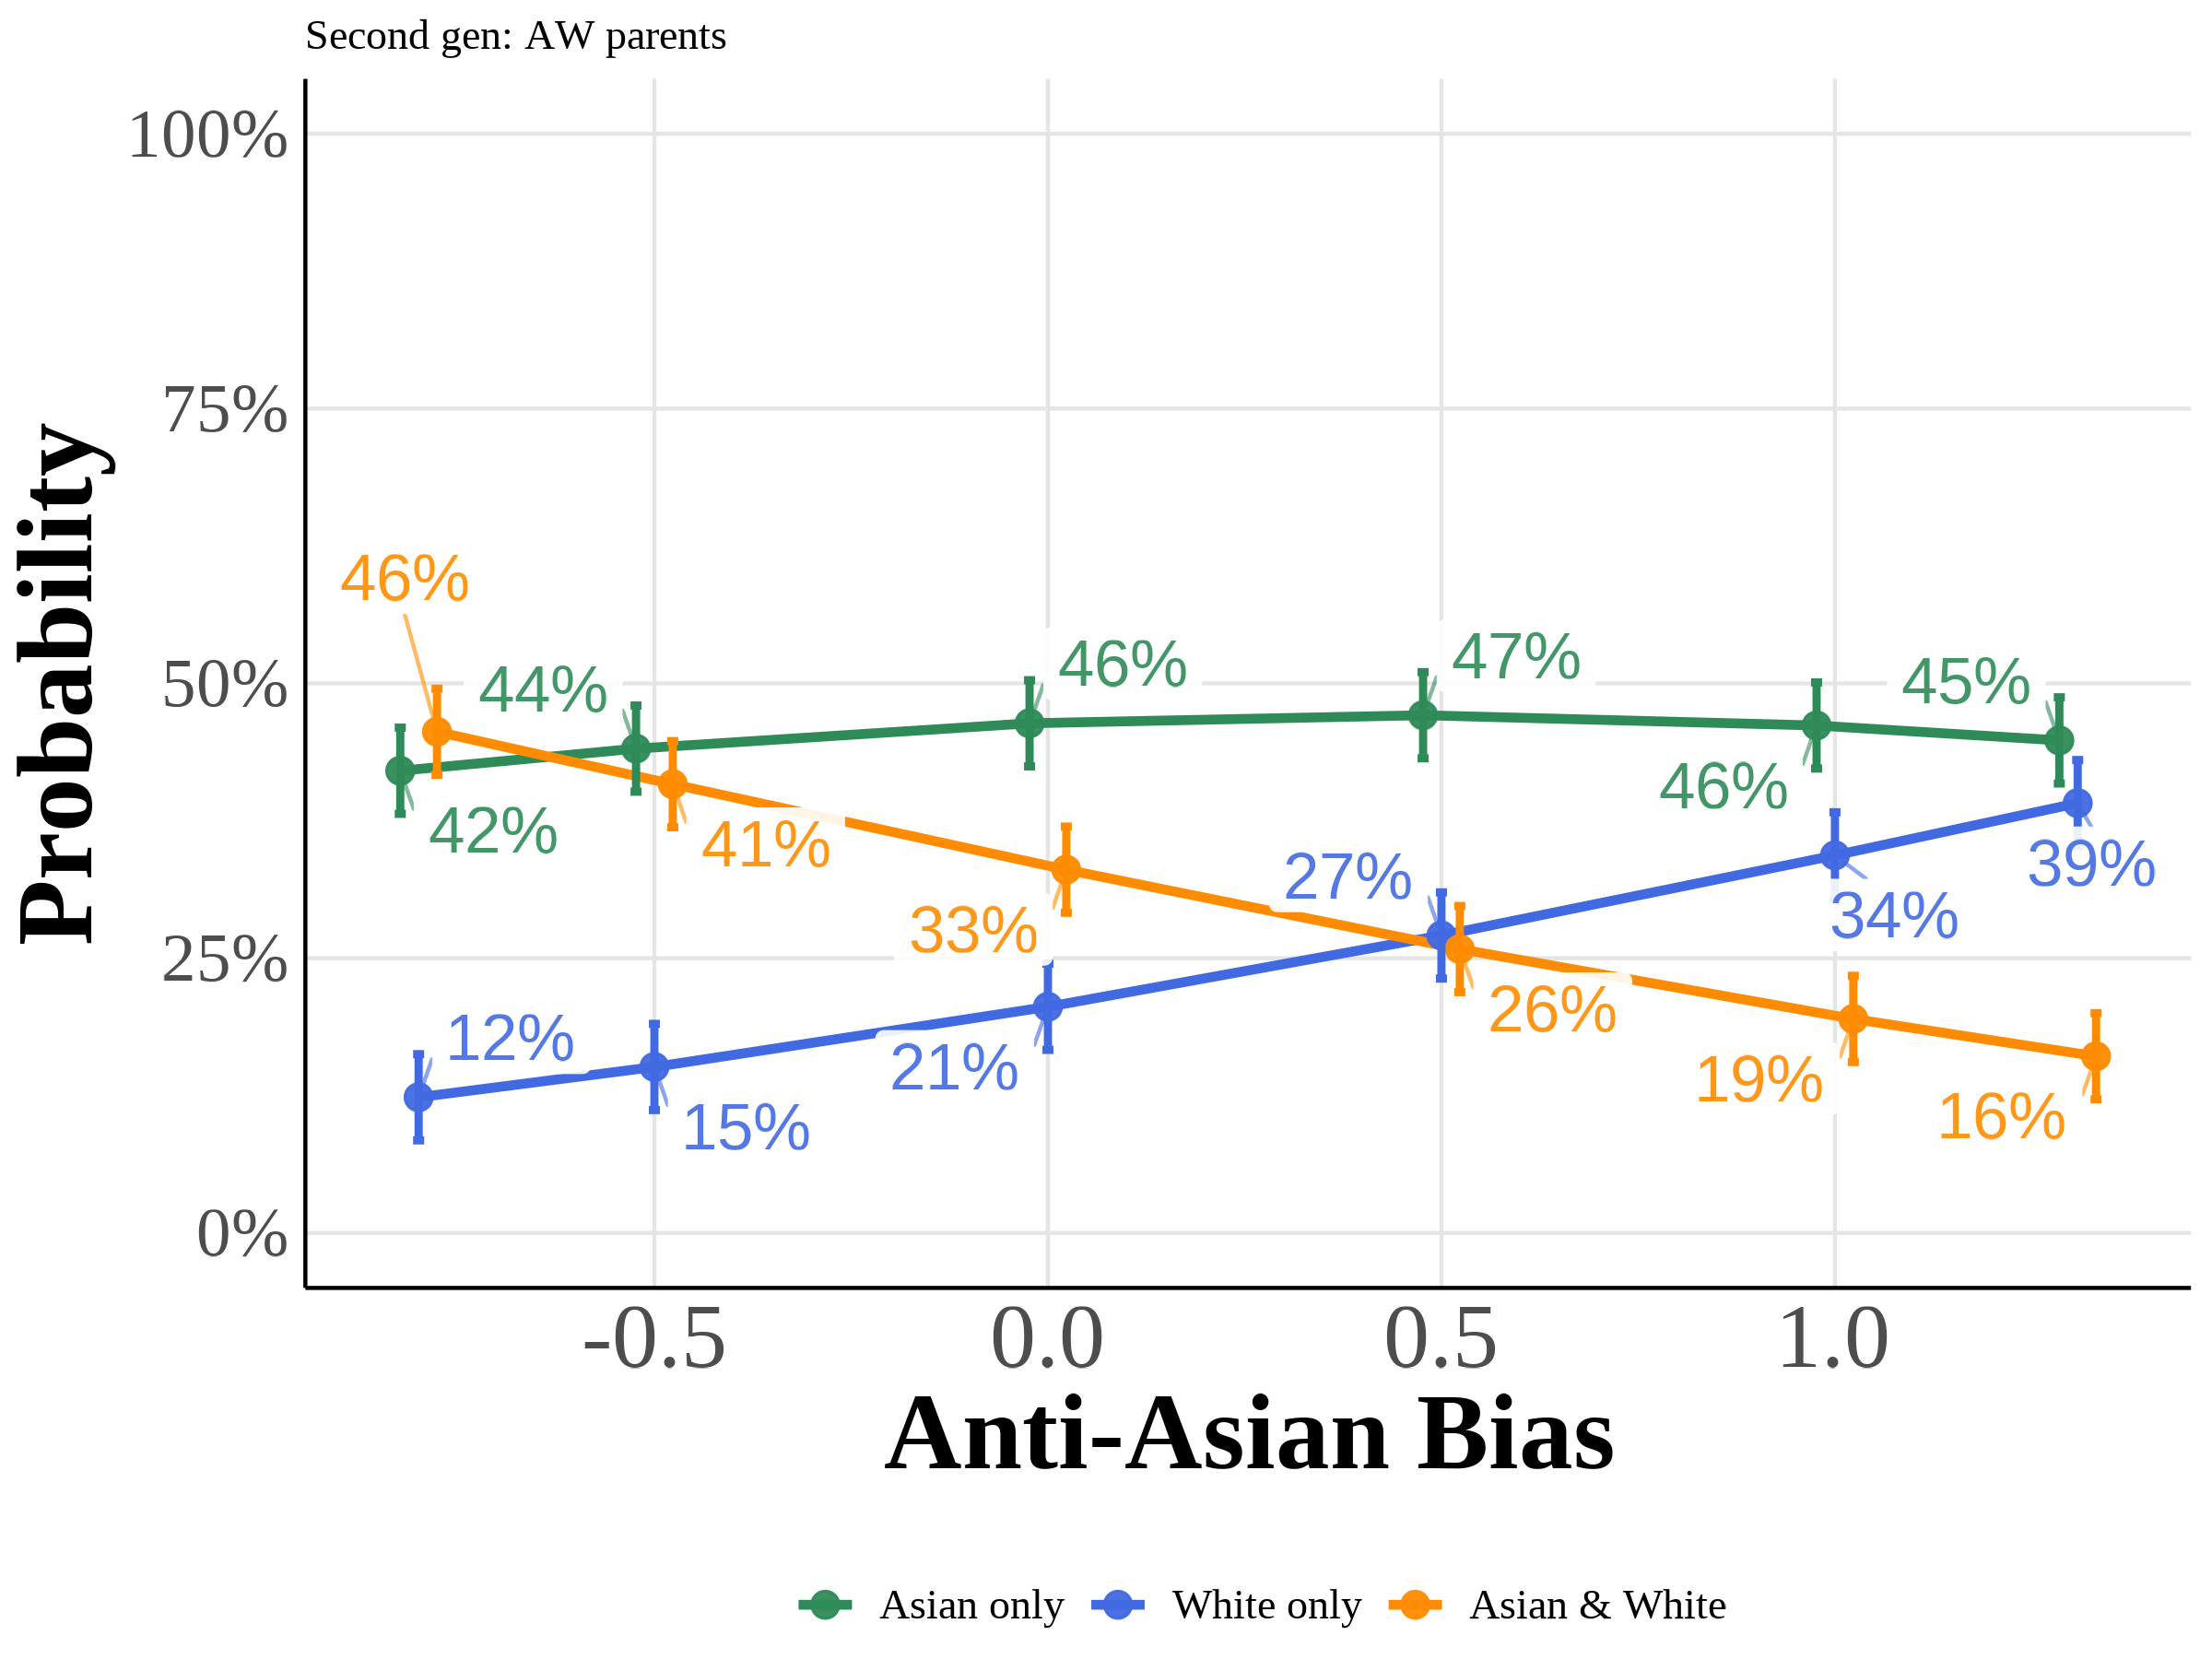
\includegraphics[width=1\linewidth]{pp_second_aw_value_simple.png}\label{subfig:pp-secgen-aw-bias}
\end{subfigure}
\hfill
\begin{subfigure}{.48\textwidth}
\caption{Anti-Asian Bias (WA)}
\centering
\includegraphics[width=1\linewidth]{pp_second_wa_value_simple.png}\label{subfig:pp-secgen-wa-bias}
\end{subfigure}

\vspace{0.5cm}

% Second row: Female
\begin{subfigure}{.48\textwidth}
\caption{Female (AW)}
\centering
\includegraphics[width=1\linewidth]{pp_second_aw_Female_simple.png}\label{subfig:pp-secgen-aw-female}
\end{subfigure}
\hfill
\begin{subfigure}{.48\textwidth}
\caption{Female (WA)}
\centering
\includegraphics[width=1\linewidth]{pp_second_wa_Female_simple.png}\label{subfig:pp-secgen-wa-female}
\end{subfigure}

\caption*{\footnotesize{Predicted probabilities from multinomial logit models for second-generation adults with Asian father/White mother (AW) and White father/Asian mother (WA). Each panel shows the probability of choosing each racial identity as a function of anti-Asian bias or gender, holding other covariates at their means.}}
\end{figure}
\end{center}

\pagebreak
\newpage

\begin{center}
\begin{figure}[!htb]
\centering
\caption{Multinomial Logit Model: Predicted Probabilities of Racial Identity Choice by Key Covariates (Third-Generation Asian Americans with One Asian Grandparent)}
\label{fig:pp-third-one}

\begin{subfigure}{.48\textwidth}
\caption{Anti-Asian Bias}
\centering
\includegraphics[width=1\linewidth]{simple_pp_value_third_one.png}
\end{subfigure}
\hfill
\begin{subfigure}{.48\textwidth}
\caption{Female}
\centering
\includegraphics[width=1\linewidth]{simple_pp_Female_third_one.png}
\end{subfigure}

\vspace{0.5cm}

\begin{subfigure}{.48\textwidth}
\caption{College Graduate: Mother}
\centering
\includegraphics[width=1\linewidth]{simple_pp_MomGradCollege_third_one.png}
\end{subfigure}
\hfill
\begin{subfigure}{.48\textwidth}
\caption{College Graduate: Father}
\centering
\includegraphics[width=1\linewidth]{simple_pp_DadGradCollege_third_one.png}
\end{subfigure}

\caption*{\footnotesize{This figure shows predicted probabilities from estimating equation (\ref{eq:multinomial_logit}) using a multinomial logit model for the subsample of third-generation Asian Americans with one Asian grandparent. The model estimates the probability of choosing ``Asian only'', ``White only'', or ``Asian and White'' racial identification as a function of anti-Asian bias, gender, and parental education. I include region $\times$ year fixed effects with controls for quartic age and local Asian population share. All other variables are held at their sample means.}}
\end{figure}
\end{center}

\pagebreak
\newpage

\begin{center}
\begin{figure}[!htb]
\centering
\caption{Multinomial Logit Model: Predicted Probabilities of Racial Identity Choice by Key Covariates (Third-Generation Asian Americans with Two Asian Grandparents)}
\label{fig:pp-third-two}

\begin{subfigure}{.48\textwidth}
\caption{Anti-Asian Bias}
\centering
\includegraphics[width=1\linewidth]{simple_pp_value_third_two.png}
\end{subfigure}
\hfill
\begin{subfigure}{.48\textwidth}
\caption{Female}
\centering
\includegraphics[width=1\linewidth]{simple_pp_Female_third_two.png}
\end{subfigure}

\vspace{0.5cm}

\begin{subfigure}{.48\textwidth}
\caption{College Graduate: Mother}
\centering
\includegraphics[width=1\linewidth]{simple_pp_MomGradCollege_third_two.png}
\end{subfigure}
\hfill
\begin{subfigure}{.48\textwidth}
\caption{College Graduate: Father}
\centering
\includegraphics[width=1\linewidth]{simple_pp_DadGradCollege_third_two.png}
\end{subfigure}

\caption*{\footnotesize{This figure shows predicted probabilities from estimating equation (\ref{eq:multinomial_logit}) using a multinomial logit model for the subsample of third-generation Asian Americans with two Asian grandparents. The model estimates the probability of choosing ``Asian only'', ``White only'', or ``Asian and White'' racial identification as a function of anti-Asian bias, gender, and parental education. I include region $\times$ year fixed effects with controls for quartic age and local Asian population share. All other variables are held at their sample means.}}
\end{figure}
\end{center}

\pagebreak
\newpage

\begin{center}
\begin{figure}[!htb]
\centering
\caption{Multinomial Logit Model: Predicted Probabilities of Racial Identity Choice by Key Covariates (Third-Generation Asian Americans with Three Asian Grandparents)}
\label{fig:pp-third-three}

\begin{subfigure}{.48\textwidth}
\caption{Anti-Asian Bias}
\centering
\includegraphics[width=1\linewidth]{simple_pp_value_third_three.png}
\end{subfigure}
\hfill
\begin{subfigure}{.48\textwidth}
\caption{Female}
\centering
\includegraphics[width=1\linewidth]{simple_pp_Female_third_three.png}
\end{subfigure}

\vspace{0.5cm}

\begin{subfigure}{.48\textwidth}
\caption{College Graduate: Mother}
\centering
\includegraphics[width=1\linewidth]{simple_pp_MomGradCollege_third_three.png}
\end{subfigure}
\hfill
\begin{subfigure}{.48\textwidth}
\caption{College Graduate: Father}
\centering
\includegraphics[width=1\linewidth]{simple_pp_DadGradCollege_third_three.png}
\end{subfigure}

\caption*{\footnotesize{This figure shows predicted probabilities from estimating equation (\ref{eq:multinomial_logit}) using a multinomial logit model for the subsample of third-generation Asian Americans with three Asian grandparents. The model estimates the probability of choosing ``Asian only'', ``White only'', or ``Asian and White'' racial identification as a function of anti-Asian bias, gender, and parental education. I include region $\times$ year fixed effects with controls for quartic age and local Asian population share. All other variables are held at their sample means.}}
\end{figure}
\end{center}

\pagebreak
\newpage

% Marginal Effects: Third Generation by Grandparental Type (One, Two, Three Asian Grandparents)
% \begin{center}
% \begin{figure}[!htb]
% \centering
% \caption{Marginal Effects of Key Covariates on Racial Identity Choice by Number of Asian Grandparents (Third-Generation Asian Americans)}
% \label{fig:marginal-effects-third-grandparental}
% \begin{subfigure}{.45\textwidth}
% \caption{One Asian Grandparent}\label{subfig:oneasiangrand}
% \centering
% \includegraphics[width=1\linewidth]{optimized_marginal_effects_third_one.png}
% \end{subfigure}
% \hfill
% \begin{subfigure}{.45\textwidth}
% \caption{Two Asian Grandparents}\label{subfig:twoasiangrand}
% \centering
% \includegraphics[width=1\linewidth]{optimized_marginal_effects_third_two.png}
% \end{subfigure}

% \vspace{0.5cm}

% \begin{subfigure}{.45\textwidth}
% \caption{Three Asian Grandparents}\label{subfig:threeasiangrand}
% \centering
% \includegraphics[width=1\linewidth]{optimized_marginal_effects_third_three.png}
% \end{subfigure}
% \caption*{\footnotesize{This figure displays the marginal effects of key covariates on the probability of each racial identification outcome, estimated from equation (\ref{eq:multinomial_logit}) using multinomial logit models for third-generation Asian Americans by number of Asian grandparents. Marginal effects represent the change in predicted probability for a one-unit increase in the covariate (or discrete change from 0 to 1 for binary variables), holding other variables at their sample means. I include region $\times$ year fixed effects with controls for quartic age and local Asian population share. Error bars indicate 95\% confidence intervals.}}
% \end{figure}
% \end{center}

% \pagebreak
% \newpage
